\documentclass[a4paper,12pt]{report}
\usepackage[a4paper,margin=2.5cm]{geometry}
\usepackage{graphicx}
\usepackage[colorlinks=true, linkcolor=black]{hyperref}
\usepackage{amsmath}
\usepackage{amsfonts} 
\usepackage{booktabs}
\usepackage{caption}
\usepackage{float}
\usepackage{xcolor}
\usepackage[most]{tcolorbox}
\usepackage{xcolor}
\usepackage{fancyvrb}
\usepackage{pgfplots}
\usepackage{ragged2e} %Per poter giustificare il testo
\usepackage{amsthm}  %Per i teoremi
\usepackage{amssymb}


\newtheorem{theorem}{Teorema} %Definire i teoremi

\captionsetup{font=it} %Tutte le didascalie delle immagini in corsivo

\definecolor{darkgreen}{RGB}{0,100,0} %definiamo il colore
\pgfplotsset{compat=1.18}


%Questo comando mi permette di evidenziare in giallo le formule più importanti
\newcommand{\highlight}[1]{%
\colorbox{yellow!20}{$\displaystyle #1$}%
}

\DefineVerbatimEnvironment  %definisco un font e un colore specifico per lo pseudocode
{pseudocode}
{Verbatim}
{formatcom=\color{darkgreen}, fontsize=\small}


% Dati
\title{\textbf{Machine Learning}}
\author{Sara Cristina Basco}
\date{\today}

\begin{document}

\maketitle

\tableofcontents
\clearpage

\chapter{Introduzione al Machine Learning}

\section{Definizione di Machine Learning}

Il \textit{Machine Learning} (ML) può essere definito come il campo di studio che si occupa di programmare calcolatori affinché migliorino la loro performance su un determinato compito attraverso l'esperienza.
Formalmente, un sistema di apprendimento migliora la propria prestazione rispetto a un compito $T$, misurata da una metrica di performance $P$, sulla base dell’esperienza $E$.

\[
\text{Learning} \equiv \text{Improve}(T, P, E)
\]

Il Machine Learning è particolarmente utile quando:
\begin{itemize}
    \item non esiste una competenza umana esplicita;
    \item gli esseri umani non sono in grado di formalizzare la propria esperienza;
    \item la soluzione deve adattarsi a casi specifici o a dati in continua evoluzione.
\end{itemize}

\section{Fattori abilitanti del Machine Learning}

Lo sviluppo del Machine Learning è stato reso possibile dalla convergenza di tre fattori principali:
\begin{itemize}
    \item progressi teorici e algoritmici;
    \item disponibilità massiva di dati (Big Data);
    \item aumento della potenza computazionale, in particolare grazie alle GPU.
\end{itemize}

\section{Applicazioni del Machine Learning}

Il Machine Learning trova applicazione in numerosi domini, tra cui:
\begin{itemize}
    \item computer vision;
    \item riconoscimento vocale e interazione parlata;
    \item analisi di testi e documenti;
    \item data analytics;
    \item controllo robotico;
    \item giochi e sistemi decisionali.
\end{itemize}

\section{Cos’è un problema di apprendimento}

Un problema di apprendimento consiste nel migliorare una prestazione nel tempo grazie all’esperienza.
Un classico esempio è l’apprendimento del gioco della dama:

\begin{itemize}
    \item Compito ($T$): giocare a dama;
    \item Performance ($P$): percentuale di partite vinte;
    \item Esperienza ($E$): partite giocate contro sé stessi.
\end{itemize}

La progettazione di un sistema di apprendimento richiede di rispondere alle seguenti domande:
\begin{itemize}
    \item quale esperienza utilizzare;
    \item cosa deve essere appreso;
    \item come rappresentare la conoscenza;
    \item quale algoritmo usare per apprendere.
\end{itemize}

\section{Funzione ideale}

In un problema di apprendimento si assume l’esistenza di una funzione ideale che descrive perfettamente il comportamento desiderato.
Tale funzione è concettualmente corretta, ma non è disponibile in forma esplicita e non è computabile nella pratica.

Nel caso generale, si tratta di una funzione:
\[
f : X \rightarrow Y
\]

che associa a ogni possibile istanza di input \( x \in X \) l’output corretto \( y \in Y \).
L’obiettivo del Machine Learning è apprendere una funzione che approssimi il più possibile questa funzione ideale, utilizzando un insieme finito di esempi.

\section{Funzione valore}

Nel problema dell’apprendimento del gioco della dama, la funzione ideale può essere espressa tramite una funzione valore:
\[
V(b)
\]

che associa a ogni configurazione della scacchiera \( b \) un valore reale che rappresenta la qualità della posizione.

Una possibile definizione concettuale della funzione valore è la seguente:
\begin{itemize}
    \item se \( b \) è uno stato finale vinto, allora \( V(b) = 100 \);
    \item se \( b \) è uno stato finale perso, allora \( V(b) = -100 \);
    \item se \( b \) è uno stato finale di pareggio, allora \( V(b) = 0 \);
    \item se \( b \) non è uno stato finale, allora \( V(b) \) è il valore del miglior stato finale raggiungibile giocando in modo ottimale.
\end{itemize}

Questa funzione è corretta dal punto di vista teorico, ma non è computabile, poiché richiederebbe di esplorare completamente lo spazio degli stati e delle possibili partite.

\subsection{Rappresentazione approssimata della funzione valore}

Poiché la funzione valore ideale \( V(b) \) non è computabile, si introduce una funzione approssimata \( \hat V(b) \), appartenente a una classe di funzioni più semplici e computabili.

Nel caso considerato, \( \hat V(b) \) è rappresentata come una combinazione lineare di feature estratte dalla configurazione della scacchiera:
\[
\hat V(b) = w_0 + \sum_{i=1}^{n} w_i \, f_i(b)
\]

dove:
\begin{itemize}
    \item \( f_i(b) \) sono feature note e computabili;
    \item \( w_i \) sono coefficienti reali ignoti;
    \item \( \hat V(b) \) approssima il valore reale della configurazione.
\end{itemize}

Nel caso specifico della dama, le feature includono il numero di pedine, dame e pezzi minacciati per ciascun giocatore.
L’apprendimento si riduce quindi alla stima dei pesi \( w_i \).

\section{Algoritmo di apprendimento}

L’apprendimento dei pesi \( w_i \) avviene tramite un algoritmo iterativo basato sulla riduzione dell’errore tra il valore stimato e il valore di training.

Nel caso considerato viene utilizzato l’algoritmo \textit{LMS (Least Mean Squares)}.

Dato un esempio di training \( b \), l’errore è definito come:
\[
\text{error}(b) = V_{\text{train}}(b) - \hat V(b)
\]

I pesi vengono aggiornati secondo la regola:
\[
w_i \leftarrow w_i + c \cdot f_i(b) \cdot \text{error}(b)
\]

dove \( c \) è il learning rate, che controlla la velocità di apprendimento.

L’algoritmo LMS è un metodo di apprendimento incrementale basato sulla discesa del gradiente stocastica.


\section{Funzione obiettivo e rappresentazione}

Nel Machine Learning si assume l’esistenza di una funzione obiettivo (o funzione target) sconosciuta:
\[
f : X \rightarrow Y
\]

L’obiettivo dell’apprendimento è calcolare una funzione approssimata:
\[
\hat{f}(x) \approx f(x)
\]

che generalizzi correttamente anche su esempi non presenti nel dataset di training.

\section{Dataset e generalizzazione}

Dato un dataset di addestramento:
\[
D = \{(x_i, y_i)\}_{i=1}^{n}
\]

il sottoinsieme degli input osservati è:
\[
X_D \subset X \quad \text{con} \quad |X_D| \ll |X|
\]

Il vero obiettivo dell’apprendimento non è la correttezza su $D$, ma la capacità di generalizzare a nuovi campioni $x \notin X_D$.

\section{Tipologie di problemi di Machine Learning}

In base al tipo di dataset e di output, si distinguono tre principali categorie:

\subsection{Supervised Learning}

Il dataset contiene coppie input-output:
\[
D = \{(x_i, y_i)\}_{i=1}^{n}
\]

Include:
\begin{itemize}
    \item \textbf{Classificazione}: $Y = \{C_1, \dots, C_k\}$;
    \item \textbf{Regressione}: $Y \subset \mathbb{R}^k$.
\end{itemize}

Caso particolare: \textbf{Concept Learning}, con output binario $Y = \{0,1\}$.

\subsection{Unsupervised Learning}

Il dataset contiene solo input:
\[
D = \{x_i\}_{i=1}^{n}
\]

L’obiettivo è individuare strutture latenti nei dati, come nel clustering o nella riduzione dimensionale.

\subsection{Reinforcement Learning}

Il sistema apprende una politica:
\[
\pi : S \rightarrow A
\]

sulla base di sequenze di stati, azioni e ricompense:
\[
D = \{(s_0, a_1, r_1, s_1, \dots)\}
\]

Non è disponibile un output supervisionato diretto, ma solo ricompense sparse e ritardate.

\section{Ipotesi e spazio delle ipotesi}

Un’ipotesi \( h \) è una possibile approssimazione della funzione target ideale.
Ogni ipotesi rappresenta una funzione che associa a ciascuna istanza di input un valore di output.

Lo \textbf{spazio delle ipotesi} \( H \) è l’insieme di tutte le ipotesi che il sistema di apprendimento è in grado di rappresentare, dato un certo formalismo o modello scelto.

L’apprendimento può essere visto come un problema di ricerca nello spazio delle ipotesi, in cui si vuole individuare l’ipotesi che massimizza una misura di performance sul dataset di training:
\[
h^* = \arg\max_{h \in H} \text{Performance}(h, D)
\]

La scelta dello spazio delle ipotesi è cruciale, poiché determina:
\begin{itemize}
    \item il potere rappresentativo del modello;
    \item la capacità di generalizzazione;
    \item la complessità computazionale del processo di apprendimento.
\end{itemize}

Uno spazio delle ipotesi troppo limitato può non contenere una buona approssimazione della funzione target, mentre uno spazio troppo ampio può portare a scarsa generalizzazione.


\section{Consistenza e Version Space}

Un’ipotesi \( h \) si dice \textbf{consistente} con un dataset di training \( D \) se fornisce la risposta corretta per tutti gli esempi presenti nel dataset:
\[
\forall (x, c(x)) \in D \quad h(x) = c(x)
\]

Il \textbf{Version Space} è definito come il sottoinsieme dello spazio delle ipotesi contenente tutte le ipotesi consistenti con i dati osservati:
\[
VS_{H,D} = \{ h \in H \mid h \text{ è consistente con } D \}
\]

Il Version Space rappresenta l’insieme di tutte le spiegazioni compatibili con i dati disponibili.
L’obiettivo di un sistema di apprendimento non è semplicemente trovare una qualunque ipotesi consistente, ma selezionare un’ipotesi che generalizzi correttamente anche su istanze non presenti nel dataset.

\subsection*{Schema concettuale}

\begin{center}
\begin{tabular}{c}
Spazio delle istanze \( X \) \\
\(\Downarrow\) \\
Funzione target ideale \( c \) (sconosciuta) \\
\(\Downarrow\) \\
Spazio delle ipotesi \( H \) \\
\(\Downarrow\) \\
Version Space \( VS_{H,D} \subseteq H \) \\
\(\Downarrow\) \\
Ipotesi selezionata \( h^* \)
\end{tabular}
\end{center}

\section{Algoritmo List-Then-Eliminate}

Un modo concettualmente semplice per calcolare il Version Space è l’algoritmo \textit{List-Then-Eliminate}.
Questo algoritmo assume che lo spazio delle ipotesi \( H \) sia finito ed enumerabile.

L’algoritmo opera come segue:
\begin{enumerate}
    \item inizializza il Version Space contenendo tutte le ipotesi in \( H \);
    \item per ogni esempio di training \( (x, c(x)) \), elimina dal Version Space tutte le ipotesi \( h \) tali che \( h(x) \neq c(x) \);
    \item restituisce l’insieme delle ipotesi rimanenti nel Version Space.
\end{enumerate}

Formalmente:
\[
VS_{H,D} = \{ h \in H \mid \forall (x, c(x)) \in D,\; h(x) = c(x) \}
\]

\subsection{Osservazioni}

L’algoritmo List-Then-Eliminate è corretto dal punto di vista teorico, ma non è utilizzabile nella pratica, poiché richiede l’enumerazione esplicita di tutte le ipotesi in \( H \).

Il suo ruolo principale è quello di chiarire:
\begin{itemize}
    \item il concetto di consistenza;
    \item il significato operativo di Version Space;
    \item il legame tra dati di training e riduzione dello spazio delle ipotesi.
\end{itemize}

\subsection*{Schema concettuale}

\begin{center}
\begin{tabular}{c}
Inizialmente: \( VS = H \) \\
\(\Downarrow\) \\
Arrivo di un esempio di training \\
\(\Downarrow\) \\
Eliminazione delle ipotesi inconsistenti \\
\(\Downarrow\) \\
Version Space progressivamente più piccolo
\end{tabular}
\end{center}


\section{Rappresentazione vs Generalizzazione}

Esiste un compromesso fondamentale tra:
\begin{itemize}
    \item \textbf{potere rappresentativo} dello spazio delle ipotesi;
    \item \textbf{potere di generalizzazione}.
\end{itemize}

Se lo spazio delle ipotesi è troppo potente (può rappresentare ogni sottoinsieme di $X$), il sistema perde capacità di generalizzare.

\section{Dati rumorosi}

Nei problemi reali, il dataset può contenere rumore:
\[
y_i \neq c(x_i)
\]

In questi casi:
\begin{itemize}
    \item il Version Space può essere vuoto;
    \item non esistono ipotesi perfettamente consistenti;
    \item è necessario adottare metodi statistici robusti.
\end{itemize}

\section*{RIEPILOGO}

\begin{center}
\colorbox{green!10}{
\begin{minipage}{0.95\textwidth}

\textbf{Machine Learning} è un approccio \textit{data-driven} che si basa sull’uso dei dati per costruire modelli quando una descrizione completa dell’ambiente non è disponibile.
L’apprendimento è definito come il miglioramento delle prestazioni su un compito, sulla base dell’esperienza e misurato tramite una metrica di performance.

Nel Machine Learning si assume l’esistenza di una funzione ideale (target) sconosciuta, che viene approssimata mediante una funzione computabile.
Nel caso dell’apprendimento del gioco della dama, tale funzione è una funzione valore \( V(b) \), che assegna a ogni configurazione un valore numerico.
Poiché \( V(b) \) non è computabile, si introduce una funzione approssimata \( \hat V(b) \), rappresentata come combinazione lineare di feature, i cui parametri vengono appresi dai dati.

L’apprendimento dei parametri avviene tramite un algoritmo iterativo, come l’algoritmo LMS, che aggiorna i pesi riducendo l’errore tra il valore stimato e il valore di training.

\medskip
\textbf{Tipologie di problemi di Machine Learning:}
\begin{itemize}
    \item \textbf{Supervised Learning}: il dataset contiene coppie input-output; include problemi di regressione e classificazione;
    \item \textbf{Unsupervised Learning}: il dataset contiene solo input, senza etichette; l’obiettivo è scoprire strutture latenti nei dati;
    \item \textbf{Reinforcement Learning}: l’agente apprende una politica sulla base di ricompense ritardate e interazioni con l’ambiente.
\end{itemize}

\medskip
\textbf{Notazione ricorrente:}
\begin{itemize}
    \item \( X \): spazio delle istanze;
    \item \( x \in X \): una singola istanza;
    \item \( D = \{(x_i, c(x_i))\}_{i=1}^n \): dataset di training;
    \item \( c \): funzione target ideale;
    \item \( H \): spazio delle ipotesi;
    \item \( h \in H \): ipotesi;
    \item \( h(x) \): valore stimato dall’ipotesi su \( x \).
\end{itemize}

Un’ipotesi è detta \textbf{consistente} con il dataset se fornisce la risposta corretta per tutti gli esempi di training.
Il \textbf{Version Space} è l’insieme di tutte le ipotesi consistenti con i dati osservati e rappresenta lo spazio delle soluzioni compatibili con il dataset.

La scelta dello spazio delle ipotesi è cruciale: uno spazio troppo semplice limita il potere rappresentativo, mentre uno spazio troppo complesso riduce la capacità di generalizzazione.
Trovare il giusto equilibrio è fondamentale per evitare fenomeni di \textit{underfitting} e \textit{overfitting}.

\end{minipage}
}
\end{center}

\chapter{Performance Evaluation}

\section{Introduzione alla valutazione delle prestazioni}

La valutazione delle prestazioni è il processo mediante il quale si stima la qualità di una ipotesi o di un algoritmo di apprendimento nel generalizzare a nuovi dati non osservati.

Dato che un modello di Machine Learning viene addestrato su un insieme finito di esempi, non è possibile osservare direttamente il suo comportamento sull’intera distribuzione dei dati.
La valutazione delle prestazioni fornisce quindi una \textbf{stima statistica} dell’accuratezza del modello su istanze future.

In termini generali, la valutazione delle prestazioni risponde a domande del tipo:
\begin{itemize}
    \item quanto è accurata l’ipotesi appresa?
    \item quanto è affidabile questa stima?
    \item come si confrontano due ipotesi o due algoritmi diversi?
\end{itemize}

È importante sottolineare che la valutazione delle prestazioni non restituisce un valore assoluto, ma una stima soggetta a incertezza, che dipende:
\begin{itemize}
    \item dalla quantità di dati disponibili;
    \item dalla modalità di campionamento;
    \item dalla metrica di valutazione utilizzata.
\end{itemize}

La difficoltà principale nella valutazione delle prestazioni risiede nel fatto che l’errore vero di un modello non è osservabile direttamente.
Per questo motivo si introducono stime basate su campioni finiti di dati, come l’errore campionario.

\section{Errore vero ed errore campionario}

Sia \( f : X \rightarrow Y \) la funzione target ideale e sia \( D \) una distribuzione di probabilità sugli input.
Dato un modello appreso \( h \), l’obiettivo della valutazione delle prestazioni è stimare quanto spesso \( h \) fornisca una predizione errata su esempi futuri.

\subsection{Errore vero}

L’\textbf{errore vero} di un’ipotesi \( h \) è definito come la probabilità che \( h \) commetta un errore su un’istanza estratta casualmente secondo la distribuzione \( D \):
\[
\highlight{error_D(h) = \Pr_{x \sim D}[f(x) \neq h(x)]}
\]

L’errore vero rappresenta la reale capacità di generalizzazione del modello.
Tuttavia, non può essere calcolato direttamente, poiché la distribuzione \( D \) e la funzione target \( f \) sono sconosciute.

\subsection{Errore campionario}

Poiché l’errore vero non è osservabile, si introduce l’\textbf{errore campionario}, calcolato su un insieme finito di esempi \( S \):
\[
\highlight{
error_S(h) = \frac{1}{|S|} \sum_{x \in S} \delta(f(x) \neq h(x))
}
\]

L’errore campionario è una quantità misurabile e rappresenta una stima dell’errore vero.
Tuttavia, essendo calcolato su un campione finito, dipende dagli esempi contenuti in \( S \).

\subsection*{Esempio}

Si consideri un problema di classificazione binaria e un modello \( h \).
Supponiamo di testare il modello su un insieme di 20 esempi e osservare 2 errori.
In questo caso:
\[
error_S(h) = \frac{2}{20} = 0.1
\]

Questo valore rappresenta l’errore campionario.
Tuttavia, se il test fosse stato effettuato su un diverso campione di 20 esempi estratti dalla stessa distribuzione, il numero di errori osservati avrebbe potuto essere diverso.

L’errore vero \( error_D(h) \) rappresenta invece la frazione di errori che il modello commetterebbe su un numero infinito di esempi estratti dalla distribuzione \( D \).
L’errore campionario è quindi una realizzazione casuale di una variabile aleatoria che approssima l’errore vero.

\subsection*{Interpretazione statistica}

L’errore campionario \( error_S(h) \) è una variabile casuale, poiché dipende dal campione \( S \) estratto dalla distribuzione \( D \).
Campioni diversi producono stime diverse dello stesso errore vero.

Il problema centrale della valutazione delle prestazioni consiste nel determinare:
\begin{itemize}
    \item quanto bene \( error_S(h) \) approssimi \( error_D(h) \);
    \item quanto è affidabile questa approssimazione.
\end{itemize}



\section{Intervalli di confidenza}

Se il campione di test contiene almeno 30 esempi ed è indipendente dall’ipotesi,
con probabilità approssimativamente pari a \( N\% \), l’errore vero soddisfa:
\[
error_D(h) \in error_S(h) \pm z_N
\sqrt{\frac{error_S(h)(1 - error_S(h))}{n}}
\]

dove \( z_N \) è un coefficiente dipendente dal livello di confidenza desiderato.

\section{Stima non distorta e trade-off training/testing}

Per ottenere una stima non distorta, i dati utilizzati per la valutazione devono essere indipendenti da quelli usati per l’addestramento.
Una suddivisione tipica è:
\begin{itemize}
    \item \( \frac{2}{3} \) dei dati per il training;
    \item \( \frac{1}{3} \) dei dati per il testing.
\end{itemize}

Esiste un trade-off:
più dati di training migliorano il modello, ma peggiorano la stima;
più dati di test migliorano la stima, ma peggiorano il modello.


\section{k-Fold Cross Validation}

La suddivisione dei dati in un singolo training set e un singolo test set fornisce una stima dell’errore vero, ma tale stima può avere elevata varianza, poiché dipende fortemente dalla particolare partizione dei dati.

La \textbf{k-Fold Cross Validation} è una tecnica che consente di ridurre questa variabilità, utilizzando in modo più efficiente l’intero dataset disponibile.

\subsection{Descrizione dell’algoritmo}

Dato un dataset \( D \), esso viene suddiviso in \( k \) sottoinsiemi disgiunti:
\[
D = S_1 \cup S_2 \cup \dots \cup S_k
\]

Per ogni iterazione \( i = 1, \dots, k \):
\begin{itemize}
    \item il sottoinsieme \( S_i \) viene utilizzato come test set;
    \item i rimanenti \( k-1 \) sottoinsiemi costituiscono il training set \( T_i = D \setminus S_i \);
    \item viene addestrato un modello \( h_i = L(T_i) \);
    \item viene calcolato l’errore \( error_{S_i}(h_i) \).
\end{itemize}

L’errore finale dell’algoritmo di apprendimento \( L \) è stimato come:
\[
\highlight{
error_{L,D} = \frac{1}{k} \sum_{i=1}^{k} error_{S_i}(h_i)
}
\]

\subsection*{Interpretazione}

La k-Fold Cross Validation fornisce una stima dell’\textbf{valore atteso} dell’errore campionario di un algoritmo di apprendimento.

Ogni esempio del dataset viene utilizzato:
\begin{itemize}
    \item una sola volta come dato di test;
    \item \( k-1 \) volte come dato di training.
\end{itemize}

In questo modo, la stima dell’errore:
\begin{itemize}
    \item è meno dipendente da una singola partizione dei dati;
    \item presenta una varianza inferiore rispetto a un singolo split.
\end{itemize}

\subsection*{Esempio}

Si consideri un dataset composto da 100 esempi e una 5-Fold Cross Validation.
Il dataset viene suddiviso in 5 sottoinsiemi da 20 esempi ciascuno.

Ad ogni iterazione:
\begin{itemize}
    \item 80 esempi vengono utilizzati per il training;
    \item 20 esempi vengono utilizzati per il testing.
\end{itemize}

Al termine delle 5 iterazioni, ciascun esempio è stato utilizzato esattamente una volta come test set.
L’errore finale è la media degli errori osservati nelle singole iterazioni.

\subsection*{Schema concettuale}

\begin{center}
\begin{tabular}{c}
Dataset \( D \) \\
\(\Downarrow\) \\
Suddivisione in \( k \) sottoinsiemi \( S_1, \dots, S_k \) \\
\(\Downarrow\) \\
Training e testing ripetuti \( k \) volte \\
\(\Downarrow\) \\
Media degli errori \\
\(\Downarrow\) \\
Stima dell’errore atteso dell’algoritmo
\end{tabular}
\end{center}


\section{Overfitting}

Nel Machine Learning l’obiettivo non è minimizzare l’errore sui dati di training, ma ottenere buone prestazioni su dati futuri non osservati.
Il fenomeno dell’\textbf{overfitting} si verifica quando un modello si adatta eccessivamente ai dati di training, perdendo capacità di generalizzazione.

Formalmente, data una ipotesi \( h \in H \), si dice che \( h \) presenta overfitting rispetto a un dataset \( S \) se esiste un’altra ipotesi \( h' \in H \) tale che:
\[
\highlight{
error_S(h) < error_S(h') \quad \text{e} \quad error_D(h) > error_D(h')
}
\]

In altre parole, \( h \) è migliore sui dati di training, ma peggiore sui dati futuri rispetto a \( h' \).

L’overfitting è una conseguenza di uno spazio delle ipotesi troppo complesso rispetto alla quantità di dati disponibili.
Un modello con elevato potere rappresentativo può adattarsi anche al rumore presente nel dataset, trattandolo come se fosse informazione rilevante.


\subsection*{Esempio}

Si consideri un problema di classificazione e due modelli \( h \) e \( h' \).
Il modello \( h \) è molto complesso, mentre \( h' \) è più semplice.

Supponiamo di osservare i seguenti risultati:
\[
error_S(h) = 0.02 \qquad error_S(h') = 0.08
\]
\[
error_D(h) = 0.25 \qquad error_D(h') = 0.10
\]

Il modello \( h \) commette pochissimi errori sui dati di training, ma generalizza molto male.
Al contrario, il modello \( h' \) ha un errore di training più alto, ma un errore vero più basso.

In questo caso, il modello \( h \) presenta overfitting, mentre \( h' \) rappresenta una soluzione preferibile.

L’overfitting non può essere individuato osservando esclusivamente l’errore di training.
È necessario stimare l’errore vero mediante tecniche di valutazione come il test set indipendente o la k-Fold Cross Validation.

\section{Metriche di valutazione}
\subsection{Limiti dell’accuratezza}

Nel caso di problemi di classificazione, una metrica comunemente utilizzata è l’accuratezza:
\[
Accuracy = \frac{TP + TN}{TP + TN + FP + FN}
\]

Tuttavia, l’accuratezza può risultare fuorviante in presenza di dataset sbilanciati, ovvero quando una classe è molto più frequente delle altre.
In questi casi, un classificatore banale che predice sempre la classe più frequente può ottenere un’alta accuratezza pur non essendo utile.

\subsection{Precision, Recall e F1-score}

Per valutare meglio le prestazioni in presenza di dataset sbilanciati, si introducono metriche alternative basate sulla matrice di confusione.

La \textbf{Recall} (o True Positive Rate) misura la capacità del modello di individuare correttamente i casi positivi:
\[
Recall = \frac{TP}{TP + FN}
\]

La \textbf{Precision} misura la frazione di predizioni positive corrette:
\[
Precision = \frac{TP}{TP + FP}
\]

La \textbf{F1-score} combina precision e recall in un’unica metrica:
\[
F1 = \frac{2 \cdot Precision \cdot Recall}{Precision + Recall}
\]

L’importanza relativa di precision e recall dipende dal dominio applicativo.


\subsection{Metriche derivate e curva ROC}

Altre metriche utili sono:
\begin{itemize}
    \item \textbf{True Negative Rate (Specificity)}:
    \[
    TNR = \frac{TN}{TN + FP}
    \]
    \item \textbf{False Positive Rate}:
    \[
    FPR = \frac{FP}{TN + FP}
    \]
    \item \textbf{False Negative Rate}:
    \[
    FNR = \frac{FN}{TP + FN}
    \]
\end{itemize}

La \textbf{ROC curve} rappresenta graficamente il compromesso tra True Positive Rate e False Positive Rate al variare della soglia di classificazione.
L’\textbf{AUC} (Area Under the Curve) fornisce una misura sintetica delle prestazioni complessive del classificatore.

\subsection{Dipendenza dal dominio applicativo}

L’impatto degli errori dipende fortemente dall’applicazione.
Ad esempio:
\begin{itemize}
    \item in ambito medico, un falso negativo può avere conseguenze gravi;
    \item nella guida autonoma, un falso positivo può causare frenate inutili;
    \item in sistemi di sicurezza, un falso negativo può compromettere l’intero sistema.
\end{itemize}

La scelta della metrica di valutazione deve quindi essere guidata dal contesto applicativo e non basarsi esclusivamente sull’accuratezza.

\subsection{Matrice di confusione multi-classe}

La \emph{confusion matrix} per un problema di classificazione multi-classe con $K$ classi è una matrice quadrata
\[
\mathbf{C} \in \mathbb{N}^{K \times K},
\]
in cui le righe rappresentano le classi reali e le colonne le classi predette dal classificatore.
L’elemento $C_{i,j}$ indica il numero di istanze appartenenti realmente alla classe $C_i$ che vengono classificate come appartenenti alla classe $C_j$.

La diagonale principale contiene le classificazioni corrette per ciascuna classe, mentre gli elementi fuori diagonale indicano le classi che vengono più frequentemente confuse.
L’analisi della matrice di confusione consente di individuare debolezze specifiche del classificatore.

\begin{figure}[H]
\centering
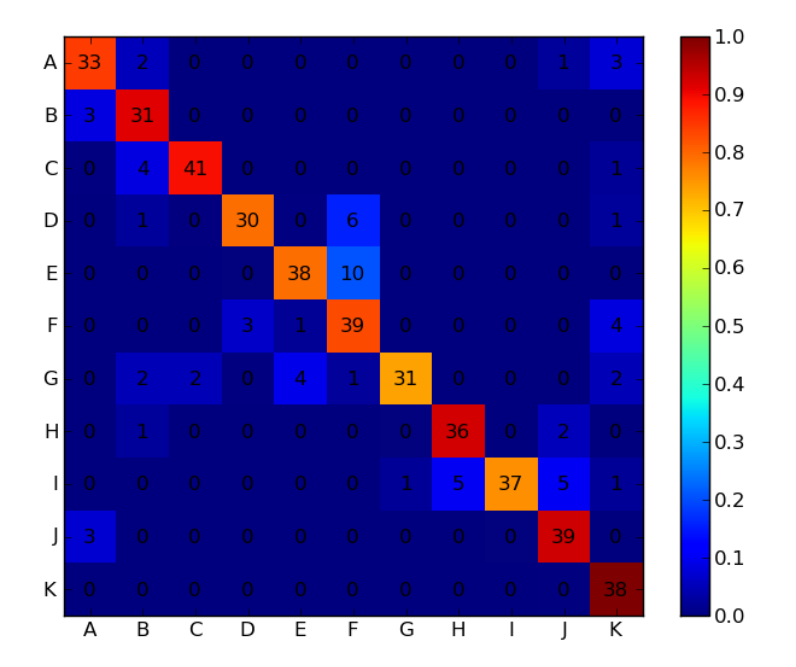
\includegraphics[width=0.55\textwidth]{confusion_matrix.png}
\caption{Esempio di matrice di confusione per un problema di classificazione. Gli elementi sulla diagonale rappresentano le predizioni corrette.}
\end{figure}

\section{Metriche di valutazione per la regressione}

Nel caso di problemi di regressione, la valutazione delle prestazioni si basa sulla differenza numerica tra il valore predetto \( \hat{f}(x_i) \) e il valore reale \( t_i \).

Le metriche più comuni sono:
\begin{itemize}
    \item \textbf{Mean Absolute Error (MAE)}:
        misura l’errore medio assoluto tra i valori predetti e i valori reali
        \[
        MAE = \frac{1}{n} \sum_{i=1}^{n} \left| \hat{f}(x_i) - t_i \right|
        \]

        Il MAE assegna lo stesso peso a tutti gli errori, indipendentemente dalla loro ampiezza.
        Ogni errore contribuisce in modo lineare alla metrica.

        \begin{figure}[H]
        \centering
        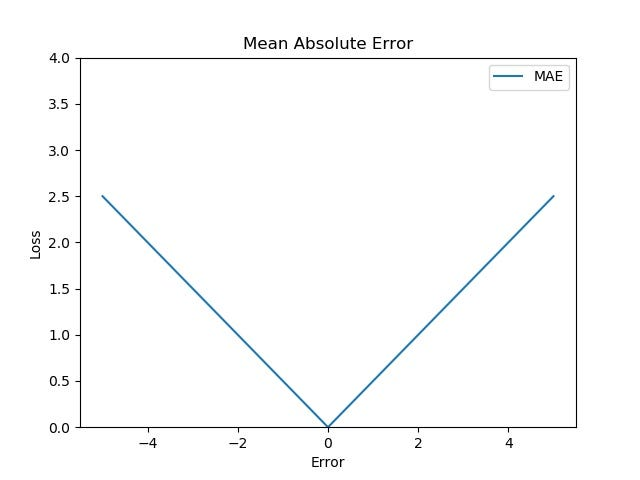
\includegraphics[width=0.70\textwidth]{MAE.jpg}
        \caption{Rappresentazione grafica del MAE.}
        \end{figure}

    \item \textbf{Mean Squared Error (MSE)}:
        è definito come
        \[
        MSE = \frac{1}{n} \sum_{i=1}^{n} \left(\hat{f}(x_i) - t_i\right)^2
        \]
        In questa metrica, gli errori vengono elevati al quadrato, penalizzando maggiormente gli errori di grande entità.

        \begin{figure}[H]
        \centering
        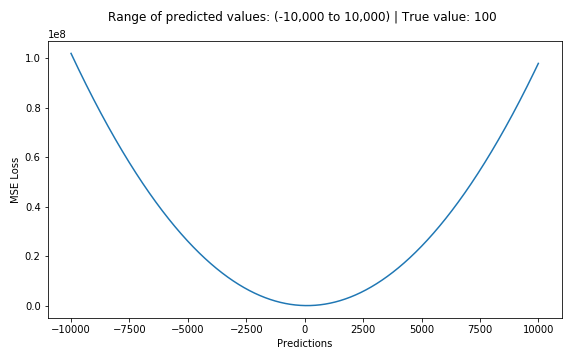
\includegraphics[width=0.70\textwidth]{MSE.png}
        \caption{Rappresentazione grafica del MSE.}
        \end{figure}

    \item \textbf{Root Mean Squared Error (RMSE)}:
        è la radice quadrata del MSE:
        \[
        RMSE = \sqrt{MSE}
        \]
        Il RMSE mantiene la sensibilità agli errori grandi tipica del MSE, ma riporta l’errore nella stessa unità di misura del target.

\subsection*{Confronto tra le metriche}

Le tre metriche differiscono per il modo in cui penalizzano gli errori:
\begin{itemize}
    \item il MAE cresce linearmente con l’errore;
    \item il MSE cresce quadraticamente;
    \item il RMSE eredita la penalizzazione del MSE, ma è più interpretabile.
\end{itemize}

\begin{figure}[H]
        \centering
        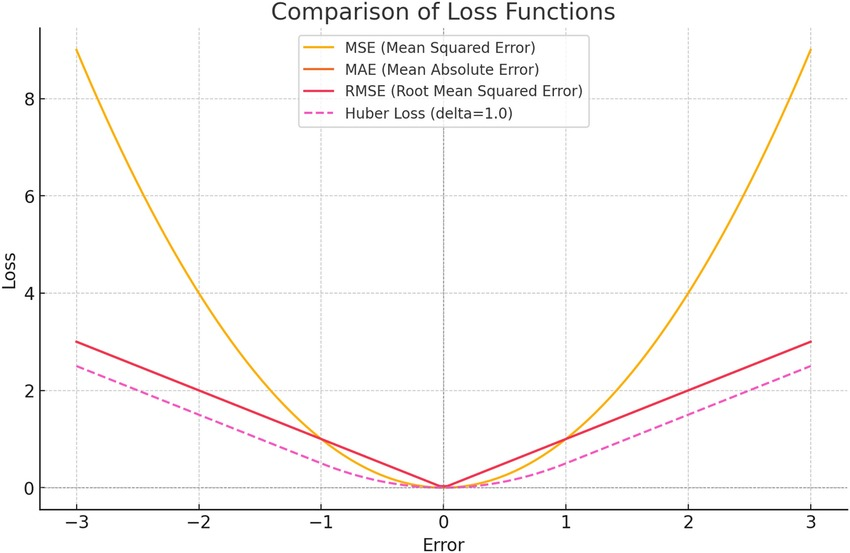
\includegraphics[width=0.70\textwidth]{confronto_metriche.jpeg}
        \caption{Rappresentazione del confronto tra le metriche.}
        \end{figure}


\end{itemize}

\subsection{Metriche percentuali e coefficiente di determinazione}

In alcuni contesti è utile valutare l’errore in termini percentuali, ad esempio tramite il Mean Absolute Percentage Error (MAPE).

Un’ulteriore metrica importante è il coefficiente di determinazione:
\[
R^2 = 1 - \frac{\sum_{i=1}^{n} (y_i - t_i)^2}{\sum_{i=1}^{n} (t_i - \mu)^2}
\quad \text{con} \quad
\mu = \frac{1}{n} \sum_{i=1}^{n} t_i
\]

Il valore \( R^2 = 0 \) corrisponde a un modello che predice sempre la media dei dati.


\subsection{Cross-validation per la regressione}

La k-Fold Cross Validation può essere estesa ai problemi di regressione utilizzando metriche appropriate, come il MAE o l’RMSE.
L’errore finale è ottenuto come media degli errori calcolati sui singoli fold.

\section*{Riepilogo}

\begin{tcolorbox}[
    colback=green!10,
    colframe=green!50!black,
    boxrule=0.4pt,
    left=6pt,
    right=6pt,
    top=6pt,
    bottom=6pt,
    breakable
]

\textbf{Valutazione delle prestazioni}  
Stima della capacità di generalizzazione di un’ipotesi o di un algoritmo su dati non osservati.

\medskip
\textbf{Errore vero ed errore campionario}
\[
\begin{aligned}
error_D(h) &= \Pr_{x \sim D}[f(x) \neq h(x)] \\
error_S(h) &= \frac{1}{|S|} \sum_{x \in S} \delta(f(x) \neq h(x))
\end{aligned}
\]

\medskip
\textbf{Train / Test split}  
I dati di valutazione devono essere indipendenti da quelli di training.

\medskip
\textbf{k-Fold Cross Validation}
\[
error_{L,D} = \frac{1}{k} \sum_{i=1}^{k} error_S(h_i)
\]
Ogni esempio è usato una volta per il test e \(k-1\) volte per il training.

\medskip
\textbf{Overfitting}
\[
error_S(h) < error_S(h') \;\land\; error_D(h) > error_D(h')
\]
Errore di training basso, errore vero alto.

\medskip
\textbf{Metriche per la classificazione}
\[
Accuracy = \frac{TP + TN}{TP + TN + FP + FN}
\]
\[
Precision = \frac{TP}{TP + FP}
\qquad
Recall = \frac{TP}{TP + FN}
\]
\[
F1 = \frac{2 \cdot Precision \cdot Recall}{Precision + Recall}
\]
ROC: TPR vs FPR — AUC misura la capacità discriminante.

\medskip
\textbf{Metriche per la regressione}
\[
MAE = \frac{1}{n} \sum_{i=1}^{n} \left| \hat{f}(x_i) - t_i \right|
\]
\[
MSE = \frac{1}{n} \sum_{i=1}^{n} \left(\hat{f}(x_i) - t_i \right)^2
\]
\[
RMSE = \sqrt{MSE}
\]
\[
R^2 = 1 -
\frac{\sum_{i=1}^{n} (\hat{f}(x_i) - t_i)^2}
{\sum_{i=1}^{n} (t_i - \mu)^2}
\]

\medskip

\end{tcolorbox}

\chapter{Decision Tree}
\section{Definizione}

Un \textit{Decision Tree} è un modello di apprendimento supervisionato che rappresenta una funzione di decisione sotto forma di struttura ad albero.
Il processo decisionale avviene mediante una sequenza di test su attributi che, partendo dalla radice, conducono a una foglia contenente la predizione finale.

Formalmente, un decision tree implementa una funzione:
\[
\highlight{
h : X \rightarrow Y }
\]
dove \( X \) rappresenta lo spazio delle istanze descritte da un insieme di attributi e \( Y \) lo spazio delle etichette di output.
Ogni cammino dalla radice a una foglia può essere interpretato come una regola di decisione del tipo:
\[
\text{IF } (condizione_1 \land condizione_2 \land \dots) \Rightarrow y
\]

\subsection{Struttura del Decision Tree}

Un decision tree è composto dai seguenti elementi fondamentali:
\begin{itemize}
    \item \textbf{Nodo radice}, che rappresenta il primo test su un attributo;
    \item \textbf{Nodi interni}, ciascuno dei quali corrisponde a un test su un attributo;
    \item \textbf{Archi}, che rappresentano i possibili esiti del test;
    \item \textbf{Foglie}, che contengono la decisione finale del modello.
\end{itemize}

Nel caso di problemi di classificazione, ogni foglia è associata a una classe, mentre nei problemi di regressione la foglia contiene un valore reale.

\begin{figure}[H]
\centering
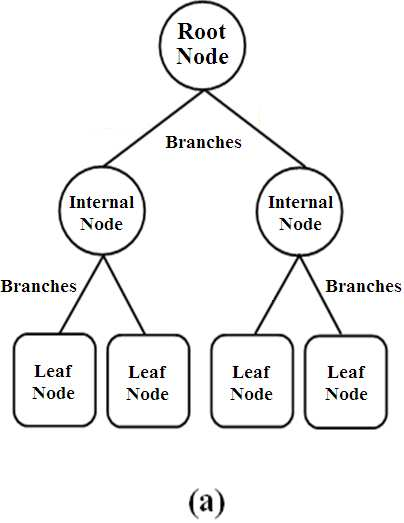
\includegraphics[width=0.65\textwidth]{decision_tree_structure.png}
\caption{Struttura generale di un decision tree: nodo radice, nodi interni e foglie.}
\end{figure}

\subsection{Caratteristiche principali}

I decision tree presentano diverse proprietà che li rendono modelli particolarmente utilizzati:

\begin{itemize}
    \item \textbf{Interpretabilità}: il modello è facilmente interpretabile, poiché il percorso seguito per effettuare una predizione è esplicito;
    \item \textbf{Assenza di assunzioni forti}: non richiedono ipotesi sulla distribuzione dei dati o relazioni lineari tra gli attributi;
    \item \textbf{Flessibilità}: possono gestire sia attributi discreti che continui;
    \item \textbf{Apprendimento non parametrico}: la complessità del modello cresce con i dati;
    \item \textbf{Rischio di overfitting}: alberi troppo profondi possono adattarsi eccessivamente ai dati di training, riducendo la capacità di generalizzazione.
\end{itemize}

\subsection*{Esempio}

Si consideri un problema di classificazione in cui l’obiettivo è decidere se giocare a tennis in base alle condizioni meteorologiche.
Gli attributi considerati sono:
\begin{itemize}
    \item \textit{Outlook} $\in$ \{Sunny, Overcast, Rain\};
    \item \textit{Humidity} $\in$ \{High, Normal\};
    \item \textit{Wind} $\in$ \{Weak, Strong\}.
\end{itemize}

La classe di output è:
\[
PlayTennis \in \{Yes, No\}
\]

Un possibile decision tree è il seguente:
\begin{itemize}
    \item se \textit{Outlook = Overcast}, allora \textit{PlayTennis = Yes};
    \item se \textit{Outlook = Sunny}:
    \begin{itemize}
        \item se \textit{Humidity = High}, allora \textit{PlayTennis = No};
        \item se \textit{Humidity = Normal}, allora \textit{PlayTennis = Yes};
    \end{itemize}
    \item se \textit{Outlook = Rain}:
    \begin{itemize}
        \item se \textit{Wind = Strong}, allora \textit{PlayTennis = No};
        \item se \textit{Wind = Weak}, allora \textit{PlayTennis = Yes}.
    \end{itemize}
\end{itemize}

\begin{figure}[H]
\centering
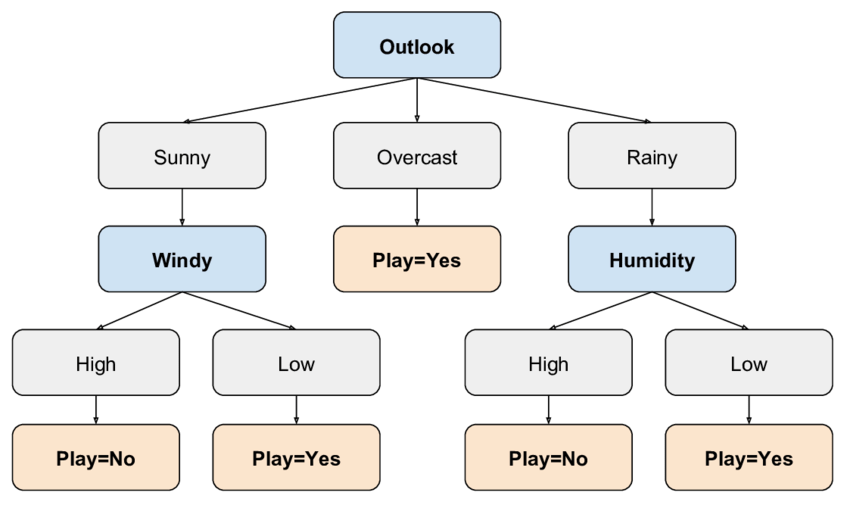
\includegraphics[width=0.65\textwidth]{play_tennis_decision_tree.png}
\caption{Esempio di decision tree per il problema Play Tennis.}
\end{figure}

\section{Regole di decisione}

Nel contesto dei decision tree, una \textbf{regola di decisione} è una proposizione logica che associa una combinazione di condizioni sugli attributi a una decisione finale.

Formalmente, una regola ha la forma:
\[
\text{IF } (condizione_1 \land condizione_2 \land \dots \land condizione_k) \Rightarrow y
\]

dove ciascuna condizione rappresenta un test su un attributo e \( y \) è il valore di output associato.

\subsection{Decision Tree come insieme di regole}

Un decision tree può essere interpretato come un insieme di regole di decisione.
Ogni cammino che parte dal nodo radice e termina in una foglia definisce una regola distinta.

Pertanto, un decision tree rappresenta una funzione di decisione equivalente a una congiunzione di regole del tipo:
\[
h(x) = \bigvee_{i=1}^{m} r_i(x)
\]
dove ciascuna regola \( r_i \) è associata a una foglia dell’albero.

\subsection{Conversione di un decision tree in regole}

La conversione di un decision tree in un insieme di regole avviene secondo i seguenti passaggi:
\begin{enumerate}
    \item si seleziona una foglia dell’albero;
    \item si considera il cammino dalla radice a tale foglia;
    \item per ogni nodo attraversato, si aggiunge alla regola la condizione associata all’arco seguito;
    \item la classe associata alla foglia costituisce la conclusione della regola.
\end{enumerate}

Ripetendo la procedura per tutte le foglie si ottiene un insieme di regole logicamente equivalenti al decision tree originale.

\begin{figure}[H]
\centering
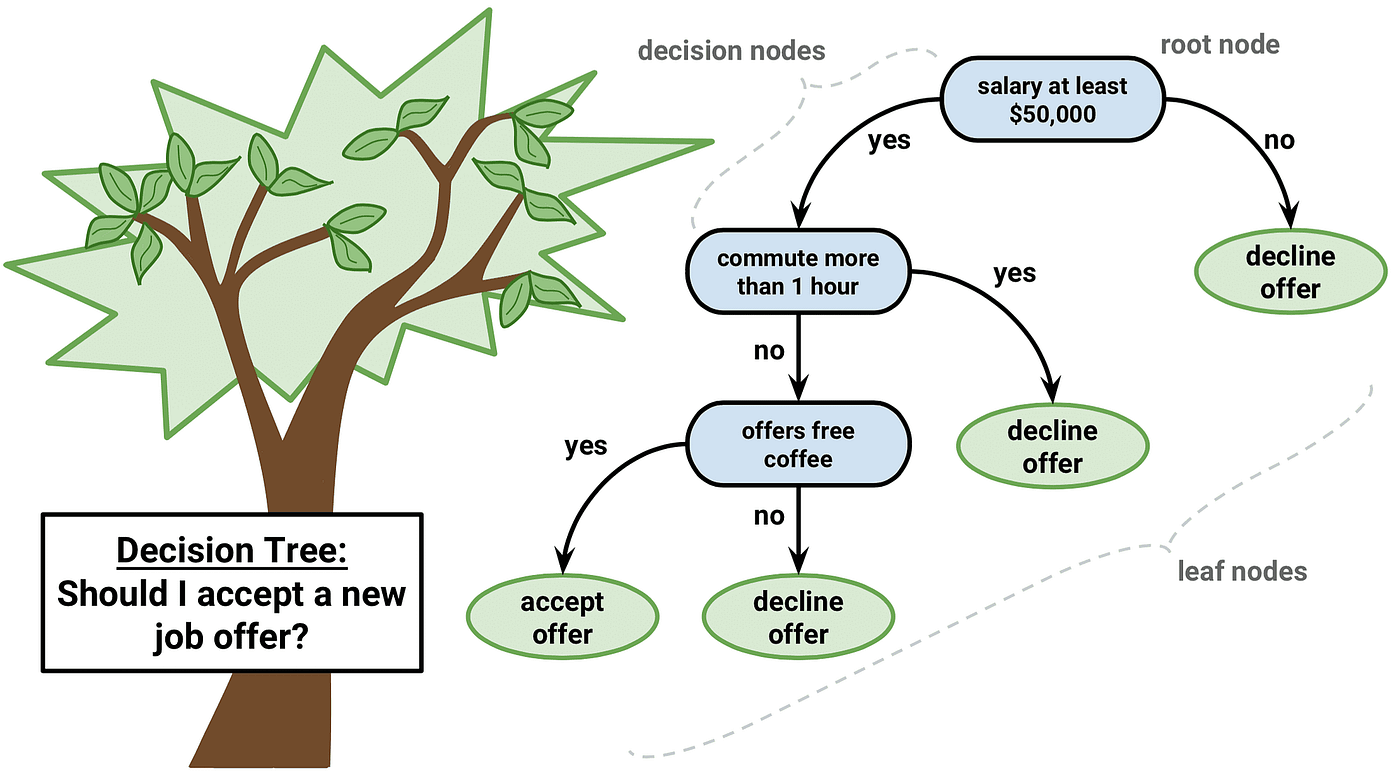
\includegraphics[width=0.7\textwidth]{decision_tree_to_rules.png}
\caption{Conversione di un decision tree in un insieme di regole: ogni percorso radice--foglia corrisponde a una regola.}
\end{figure}

\subsection*{Esempio}

Si consideri il decision tree del problema \textit{Play Tennis}.
Uno dei possibili cammini radice--foglia è il seguente:
\[
Outlook = Sunny \;\land\; Humidity = High
\]

La regola di decisione corrispondente è:
\[
\text{IF } (Outlook = Sunny \land Humidity = High) \Rightarrow PlayTennis = No
\]

Ripetendo il procedimento per ciascuna foglia dell’albero si ottiene l’insieme completo delle regole che descrivono il modello.

\subsection*{Osservazione}

Un decision tree e l’insieme di regole da esso derivato sono logicamente equivalenti.
Tuttavia, la rappresentazione a regole consente una maggiore flessibilità nella semplificazione del modello, ad esempio tramite l’eliminazione di condizioni non necessarie.

\section{Algoritmo ID3}

L’algoritmo \textit{ID3} (Iterative Dichotomiser 3) è uno dei primi algoritmi proposti per l’apprendimento di decision tree a partire da dati etichettati.
ID3 costruisce l’albero in modo incrementale, adottando una strategia \textbf{greedy top-down}, in cui ad ogni passo viene selezionato l’attributo che massimizza un criterio di bontà dello split.

L’idea alla base dell’algoritmo ID3 è quella di costruire l’albero selezionando, a ogni nodo, l’attributo che consente di separare al meglio gli esempi di training in base alle classi.

La costruzione dell’albero avviene:
\begin{itemize}
    \item partendo da tutti gli esempi nel nodo radice;
    \item scegliendo l’attributo più informativo;
    \item suddividendo il dataset in sottoinsiemi;
    \item ripetendo ricorsivamente il procedimento su ciascun sottoinsieme.
\end{itemize}

\subsection{Costruzione del decision tree}

Sia \( S \) un insieme di esempi di training e sia \( A \) l’insieme degli attributi disponibili.
L’algoritmo ID3 costruisce il decision tree secondo i seguenti passi:

\begin{enumerate}
    \item Se tutti gli esempi in \( S \) appartengono alla stessa classe, crea una foglia etichettata con tale classe.
    
    \item Se l’insieme degli attributi \( A \) è vuoto, crea una foglia etichettata con la classe più frequente in \( S \).
    
    \item Altrimenti, seleziona l’attributo \( a \in A \) che massimizza il criterio di \textit{Information Gain}.
    
    \item Crea un nodo interno etichettato con l’attributo selezionato.
    
    \item Per ciascun valore possibile \( v \) dell’attributo \( a \):
    \begin{itemize}
        \item crea un ramo corrispondente al test \( a = v \);
        \item considera il sottoinsieme \( S_v \subseteq S \) degli esempi per cui \( a = v \);
        \item applica ricorsivamente l’algoritmo ID3 a \( S_v \) e all’insieme \( A \setminus \{a\} \).
    \end{itemize}
\end{enumerate}

\subsection*{Condizioni di arresto}

La crescita dell’albero termina quando si verifica almeno una delle seguenti condizioni:
\begin{itemize}
    \item tutti gli esempi nel nodo appartengono alla stessa classe;
    \item non sono disponibili ulteriori attributi per effettuare lo split;
    \item il sottoinsieme di esempi associato al nodo è vuoto.
\end{itemize}

\subsection*{Pseudocodice}

\begin{pseudocode}
ID3(S, A):
    if tutti gli esempi in S hanno la stessa classe:
        return foglia con quella classe
    if A è vuoto:
        return foglia con la classe più frequente in S
    seleziona a in A che massimizza Information Gain
    crea un nodo con test sull’attributo a
    for ogni valore v di a:
        S_v = sottoinsieme di S con a = v
        figlio = ID3(S_v, A \ {a})
        collega figlio al nodo tramite ramo a = v
    return nodo
\end{pseudocode}


\subsection{Proprietà dell’algoritmo ID3}

L’algoritmo ID3 presenta le seguenti caratteristiche:
\begin{itemize}
    \item adotta una strategia greedy e non garantisce l’albero ottimo globale;
    \item utilizza solo attributi discreti;
    \item non prevede tecniche di pruning;
    \item è sensibile al rumore nei dati;
    \item tende a costruire alberi completi che possono soffrire di overfitting.
\end{itemize}

\subsection{ID3 e regole di decisione}

L’albero prodotto dall’algoritmo ID3 può essere convertito in un insieme di regole di decisione.
Ogni foglia dell’albero corrisponde a una regola ottenuta congiungendo le condizioni lungo il cammino radice--foglia.

\section{Entropia e Information Gain}

Nell’algoritmo ID3 è necessario stabilire quale attributo utilizzare per suddividere gli esempi in ciascun nodo dell’albero.
A tal fine viene introdotta una misura quantitativa della \textbf{purezza} di un insieme di esempi, basata su concetti di teoria dell’informazione.

\subsection{Entropia}

Sia \( S \) un insieme di esempi di training appartenenti a \( c \) classi distinte.
Si indichi con \( p_i \) la proporzione di esempi di \( S \) appartenenti alla classe \( i \).

L’\textbf{entropia} di \( S \) è definita come:
\[
\highlight{
Entropy(S) = - \sum_{i=1}^{c} p_i \log_2 p_i }
\]

L’entropia misura il grado di incertezza o impurità dell’insieme di esempi ed assume i seguenti valori caratteristici:
\begin{itemize}
    \item \( Entropy(S) = 0 \) se tutti gli esempi appartengono alla stessa classe;
    \item \( Entropy(S) \) è massima quando le classi sono equamente distribuite;
    \item valori intermedi indicano un grado parziale di impurità.
\end{itemize}

Pertanto, un insieme di esempi è tanto più informativo quanto minore è la sua entropia.

\subsection*{Esempio}

Si consideri un insieme \( S \) composto da 10 esempi, di cui 5 positivi e 5 negativi.
In questo caso:
\[
p_+ = 0.5 \qquad p_- = 0.5
\]

L’entropia risulta:
\[
Entropy(S) = -0.5 \log_2 0.5 - 0.5 \log_2 0.5 = 1
\]

Se invece tutti gli esempi appartenessero alla stessa classe, l’entropia sarebbe nulla.

\subsection{Information Gain}

L’\textbf{Information Gain} misura la riduzione di entropia ottenuta suddividendo un insieme di esempi in base a un attributo.

Dato un insieme di esempi \( S \) e un attributo \( A \) con valori possibili \( \{v_1, v_2, \dots, v_k\} \),
l’Information Gain di \( A \) rispetto a \( S \) è definito come:

\[
\highlight{
Gain(S, A) =
Entropy(S)
-
\sum_{j=1}^{k}
\frac{|S_{v_j}|}{|S|}
Entropy(S_{v_j}) }
\] 

dove \( S_{v_j} \subseteq S \) è il sottoinsieme degli esempi per cui l’attributo \( A \) assume valore \( v_j \).

L’Information Gain rappresenta la quantità di informazione ottenuta conoscendo il valore di un attributo.
Un attributo è tanto più informativo quanto maggiore è la riduzione di entropia che produce.

Pertanto, l’attributo che massimizza l’Information Gain è quello che separa meglio gli esempi in sottoinsiemi più puri.

\subsection*{Utilizzo in ID3}

Nell’algoritmo ID3, la selezione dell’attributo da utilizzare in un nodo avviene scegliendo quello che massimizza l’Information Gain.

Formalmente, dato l’insieme degli attributi disponibili \( A \), viene selezionato:
\[
\highlight{
a^* = \arg\max_{a \in A} Gain(S, a) }
\]

L’attributo selezionato viene utilizzato per suddividere il dataset e il procedimento viene applicato ricorsivamente ai sottoinsiemi generati.

\subsection{Schema operativo}

La costruzione dell’albero tramite ID3 può essere riassunta come segue:
\begin{enumerate}
    \item calcolare l’entropia dell’insieme di esempi corrente;
    \item calcolare l’Information Gain per ciascun attributo disponibile;
    \item selezionare l’attributo con massimo Information Gain;
    \item suddividere il dataset in base ai valori dell’attributo selezionato;
    \item ripetere ricorsivamente il procedimento sui sottoinsiemi ottenuti.
\end{enumerate}

\section{Overfitting nei Decision Tree}

I decision tree sono modelli altamente flessibili e possono adattarsi in modo molto accurato ai dati di training.
Tuttavia, questa flessibilità comporta un elevato rischio di \textbf{overfitting}.

Un decision tree presenta overfitting quando continua a crescere fino a classificare correttamente tutti (o quasi) gli esempi di training, includendo anche il rumore presente nei dati.
In tali casi, l’albero risulta molto accurato sui dati di training ma generalizza male su dati non osservati.

\subsection*{Definizione formale}

Dato un insieme di esempi di training \( S \), un decision tree \( h \) presenta overfitting se esiste un altro albero \( h' \) tale che:

\[
\highlight{
error_S(h) < error_S(h') \;\land\; error_D(h) > error_D(h') }
\]

In altre parole, \( h \) è migliore sui dati di training, ma peggiore sui dati futuri rispetto a \( h' \).

\subsection*{Cause principali}

Le principali cause dell’overfitting nei decision tree sono:
\begin{itemize}
    \item crescita eccessiva dell’albero;
    \item presenza di rumore nei dati di training;
    \item utilizzo di attributi poco informativi;
    \item assenza di vincoli sulla profondità dell’albero.
\end{itemize}

Poiché ID3 costruisce l’albero fino a quando è possibile separare ulteriormente gli esempi, esso tende a generare alberi completi e complessi.

\section{Pruning}

Il \textbf{pruning} è l’insieme di tecniche volte a ridurre la complessità del decision tree al fine di migliorare la capacità di generalizzazione del modello.

L’obiettivo del pruning non è minimizzare l’errore di training, bensì ridurre l’errore vero eliminando rami che modellano il rumore dei dati.

\begin{figure}[H]
\centering
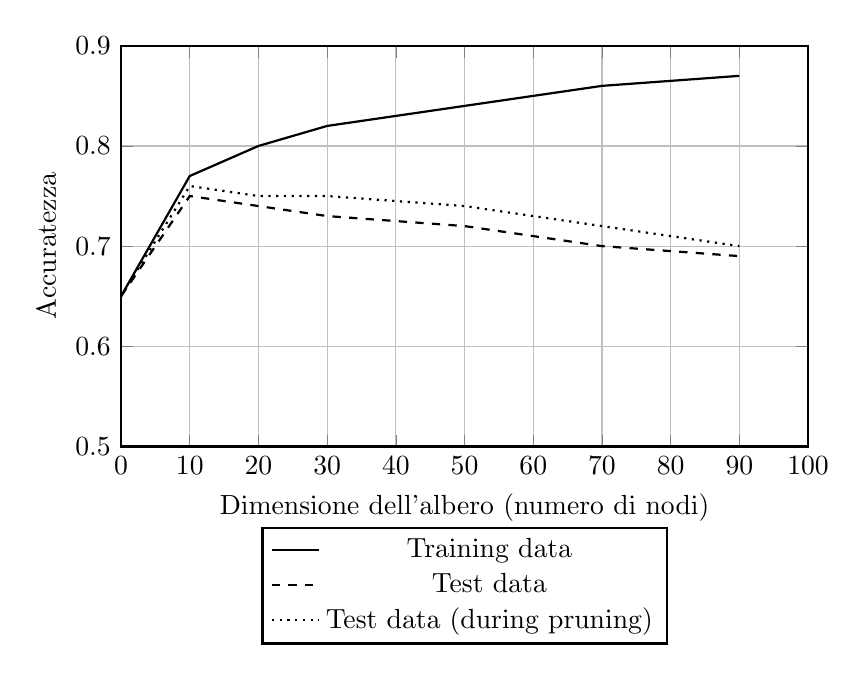
\begin{tikzpicture}
\begin{axis}[
    width=0.85\textwidth,
    height=0.55\textwidth,
    xlabel={Dimensione dell'albero (numero di nodi)},
    ylabel={Accuratezza},
    xmin=0, xmax=100,
    ymin=0.5, ymax=0.9,
    grid=both,
    legend style={at={(0.5,-0.2)},anchor=north,legend columns=1},
    thick
]

% Training accuracy
\addplot[color=black, solid] coordinates {
(0,0.65) (10,0.77) (20,0.80) (30,0.82) (50,0.84) (70,0.86) (90,0.87)
};
\addlegendentry{Training data}

% Test accuracy
\addplot[color=black, dashed] coordinates {
(0,0.65) (10,0.75) (20,0.74) (30,0.73) (50,0.72) (70,0.70) (90,0.69)
};
\addlegendentry{Test data}

% Test during pruning
\addplot[color=black, dotted] coordinates {
(0,0.65) (10,0.76) (20,0.75) (30,0.75) (50,0.74) (70,0.72) (90,0.70)
};
\addlegendentry{Test data (during pruning)}

\end{axis}
\end{tikzpicture}
\caption{Effetto del Reduced-Error Pruning: l’accuratezza sui dati di training cresce con la complessità dell’albero, mentre l’accuratezza sui dati di test mostra un massimo per una complessità intermedia.}
\end{figure}

\subsection{Pre-pruning}

Il \textbf{pre-pruning} consiste nell’interrompere la crescita dell’albero prima che esso raggiunga una struttura completa.
La decisione di arrestare la suddivisione viene presa durante la fase di costruzione dell’albero.

Criteri comuni di pre-pruning includono:
\begin{itemize}
    \item profondità massima dell’albero;
    \item numero minimo di esempi in un nodo;
    \item Information Gain inferiore a una soglia;
    \item assenza di miglioramento significativo delle prestazioni.
\end{itemize}

Il pre-pruning riduce il rischio di overfitting e il costo computazionale, ma può introdurre underfitting se applicato in modo eccessivo.

\subsection{Post-pruning}

Il \textbf{post-pruning} consiste nel costruire inizialmente un decision tree completo e successivamente semplificarlo eliminando rami poco significativi.

Il procedimento tipico di post-pruning prevede:
\begin{itemize}
    \item la valutazione delle prestazioni di un sottoalbero su un validation set;
    \item la sostituzione del sottoalbero con una foglia;
    \item il confronto tra le prestazioni prima e dopo la potatura;
    \item il mantenimento della potatura solo se migliora la generalizzazione.
\end{itemize}

Il post-pruning risulta generalmente più efficace del pre-pruning, poiché consente di valutare l’impatto reale delle potature sulla capacità di generalizzazione.

\subsection*{Confronto Pre-Pruning vs Post-Pruning}

\begin{center}
\begin{tabular}{l|c|c}
\textbf{Metodo} & \textbf{Quando applicato} & \textbf{Rischio principale} \\
\hline
Pre-pruning & Durante la crescita & Underfitting \\
Post-pruning & Dopo la crescita & Costo computazionale \\
\end{tabular}
\end{center}


\section{Random Forest}

Il \textit{Random Forest} è un metodo di apprendimento basato su un insieme di decision tree, appartenente alla famiglia dei metodi di \textbf{ensemble}.
L’idea di base è quella di combinare le predizioni di più alberi di decisione al fine di ottenere un modello più robusto e con migliori capacità di generalizzazione.

\subsection*{Idea fondamentale}

Un singolo decision tree presenta elevata varianza ed è particolarmente sensibile ai dati di training.
Il Random Forest riduce questo problema costruendo molti alberi diversi e aggregandone le predizioni.

Ogni albero viene addestrato:
\begin{itemize}
    \item su un sottoinsieme casuale degli esempi di training (bootstrap);
    \item utilizzando, a ogni nodo, un sottoinsieme casuale degli attributi disponibili.
\end{itemize}

\subsection{Aggregazione delle predizioni}

Nel caso di classificazione, la predizione finale del Random Forest è ottenuta tramite voto di maggioranza tra le predizioni dei singoli alberi.
Nel caso di regressione, la predizione finale è data dalla media delle predizioni.

Formalmente, dati \( h_1, h_2, \dots, h_T \) decision tree:
\[
\hat{y} = \text{majority\_vote}\{h_1(x), \dots, h_T(x)\}
\]

\subsection{Riduzione dell’overfitting}

Il Random Forest riduce l’overfitting combinando modelli ad alta varianza ma a basso bias.
L’introduzione di casualità nella costruzione degli alberi rende le predizioni meno correlate tra loro, migliorando la stabilità del modello complessivo.

A differenza dei singoli decision tree, il Random Forest tende a generalizzare meglio senza richiedere un pruning esplicito.

\begin{figure}[H]
\centering
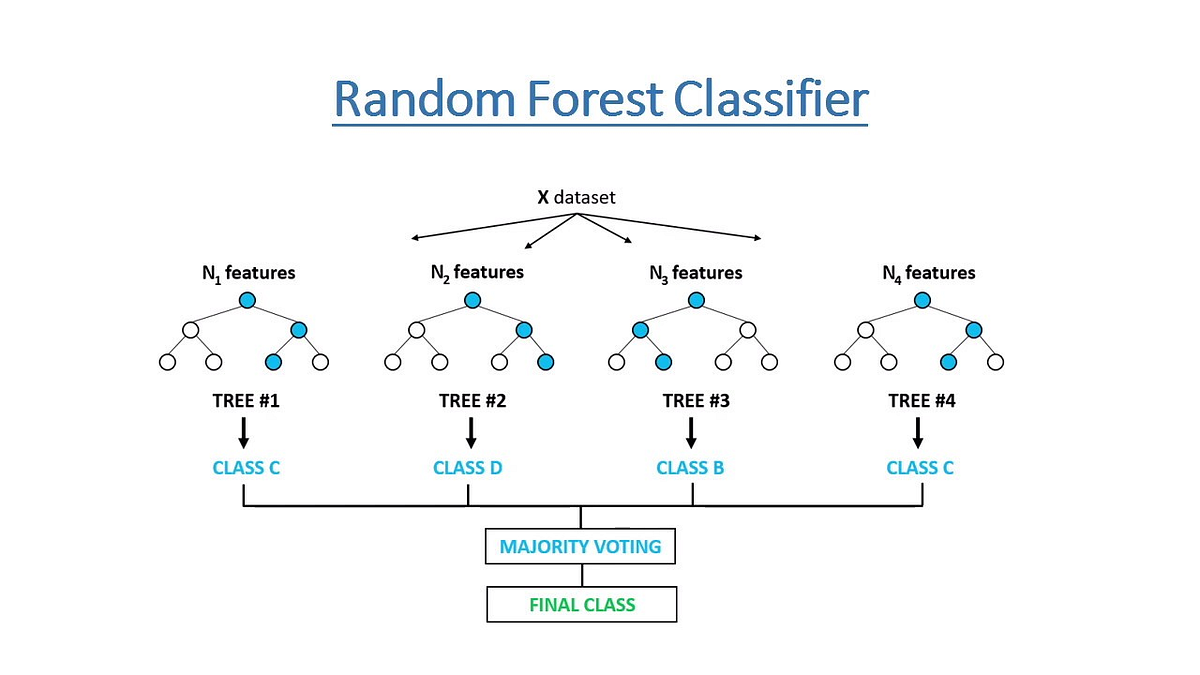
\includegraphics[width=0.98\textwidth]{random_forest.png}
\caption{Schema concettuale di un Random Forest: più decision tree addestrati su sottoinsiemi diversi dei dati e degli attributi contribuiscono alla predizione finale.}
\end{figure}

\newpage
\section*{Riepilogo}

\begin{tcolorbox}[
    colback=green!10,
    colframe=green!50!black,
    boxrule=0.4pt,
    left=6pt,
    right=6pt,
    top=6pt,
    bottom=6pt,
    breakable
]

\textbf{Decision Tree}  
Modello supervisionato che rappresenta una funzione di decisione sotto forma di struttura ad albero.
Ogni cammino radice--foglia corrisponde a una regola di decisione del tipo IF--THEN.

\medskip
\textbf{Regole di decisione}  
Un decision tree è logicamente equivalente a un insieme di regole.
Ogni foglia dell’albero definisce una regola ottenuta congiungendo le condizioni lungo il percorso radice--foglia.

\medskip
\textbf{Algoritmo ID3}  
Costruisce l’albero in modo greedy e top-down.
A ogni nodo seleziona l’attributo che massimizza l’Information Gain e suddivide ricorsivamente il dataset.
Non garantisce l’albero ottimo globale e non prevede tecniche di pruning.

\medskip
\textbf{Entropia}
\[
Entropy(S) = - \sum_{i=1}^{c} p_i \log_2 p_i
\]
Misura l’impurità di un insieme di esempi.
È nulla se tutti gli esempi appartengono alla stessa classe ed è massima quando le classi sono equamente distribuite.

\medskip
\textbf{Information Gain}
\[
Gain(S,A) = Entropy(S) - \sum_{v \in Values(A)} \frac{|S_v|}{|S|} Entropy(S_v)
\]
Misura la riduzione di entropia ottenuta suddividendo gli esempi in base a un attributo.
ID3 seleziona l’attributo con massimo Information Gain.

\medskip
\textbf{Overfitting}
Un decision tree può adattarsi eccessivamente ai dati di training, ottenendo errore campionario basso ma scarsa capacità di generalizzazione:
\[
error_S(h) < error_S(h') \;\land\; error_D(h) > error_D(h')
\]

\medskip
\textbf{Pruning}  
Tecniche volte a ridurre la complessità dell’albero per migliorare la generalizzazione.
\begin{itemize}
    \item \textit{Pre-pruning}: arresto anticipato della crescita (rischio di underfitting);
    \item \textit{Post-pruning}: potatura di un albero completo sulla base delle prestazioni su validation set.
\end{itemize}

\medskip
\textbf{Random Forest}  
Metodo ensemble che combina più decision tree addestrati su sottoinsiemi casuali di dati e attributi.
Riduce la varianza e l’overfitting dei singoli alberi, a costo di una minore interpretabilità.

\end{tcolorbox}

\section*{RIEPILOGO — Probabilità e Bayes Networks}

\begin{tcolorbox}[
    colback=green!10,
    colframe=green!50!black,
    boxrule=0.4pt,
    left=6pt,
    right=6pt,
    top=6pt,
    bottom=6pt,
    breakable
]

\textbf{Incertezza}  
In ambienti reali l’informazione è incompleta, rumorosa e parzialmente osservabile.
Un approccio puramente logico risulta inadeguato per prendere decisioni efficaci.

\medskip
\textbf{Probabilità}  
La probabilità fornisce una rappresentazione quantitativa dell’incertezza.
Uno spazio di probabilità è definito da:
\[
\Omega \text{ (spazio campionario)}, \qquad P : \Omega \rightarrow [0,1], \qquad \sum_{\omega \in \Omega} P(\omega) = 1
\]

\medskip
\textbf{Eventi e variabili casuali}  
Un evento è un sottoinsieme di \( \Omega \).
Una variabile casuale è una funzione:
\[
X : \Omega \rightarrow D(X)
\]
che induce una distribuzione di probabilità \( P(X = x_i) \).

\medskip
\textbf{Distribuzioni di probabilità}  
\begin{itemize}
    \item \textit{Distribuzione prior}: credenza prima di osservare evidenza;
    \item \textit{Distribuzione congiunta}: probabilità di tutte le combinazioni di valori delle variabili;
    \item \textit{Distribuzione condizionata}: probabilità di una variabile dato il valore di un’altra.
\end{itemize}

\medskip
\textbf{Probabilità condizionata e regola del prodotto}
\[
P(a \mid b) = \frac{P(a \land b)}{P(b)}, \qquad
P(a,b) = P(a \mid b)P(b)
\]

\medskip
\textbf{Probabilità totali}
\[
P(X) = \sum_{y \in D(Y)} P(X \mid Y=y) P(Y=y)
\]

\medskip
\textbf{Chain Rule}
\[
P(X_1,\dots,X_n) = \prod_{i=1}^{n} P(X_i \mid X_1,\dots,X_{i-1})
\]

\medskip
\textbf{Indipendenza}  
Due eventi sono indipendenti se:
\[
P(A,B) = P(A)P(B)
\]

L’indipendenza assoluta è rara nei sistemi complessi.

\medskip
\textbf{Indipendenza condizionata}  
\[
X \perp Y \mid Z \iff P(X \mid Y,Z) = P(X \mid Z)
\]
Consente una rappresentazione compatta delle distribuzioni congiunte.

\medskip
\textbf{Regola di Bayes}
\[
P(Y \mid X) = \frac{P(X \mid Y)P(Y)}{P(X)} = \alpha P(X \mid Y)P(Y)
\]
Fondamentale per il ragionamento diagnostico (cause a partire dagli effetti).

\medskip
\textbf{Massima verosimiglianza}
\[
\arg\max_{x_i \in D(X)} P(X=x_i \mid Y)
= \arg\max_{x_i} P(Y \mid X=x_i)P(X=x_i)
\]

\medskip
\textbf{Bayesian Networks}  
Modelli grafici che rappresentano variabili casuali e relazioni di dipendenza tramite:
\begin{itemize}
    \item nodi (variabili);
    \item archi diretti (dipendenze causali);
    \item CPT: \( P(X_i \mid Parents(X_i)) \).
\end{itemize}

Le reti bayesiane permettono di rappresentare distribuzioni congiunte in modo compatto, riducendo la complessità da esponenziale a lineare (a parità di genitori).

\end{tcolorbox}

\newpage

\chapter{Bayesian Learning}

\section{Motivazione}

Nel Machine Learning supervisionato, l’obiettivo principale è apprendere una funzione che consenta di effettuare predizioni corrette su nuove istanze non osservate.
Nei capitoli precedenti, l’apprendimento è stato affrontato prevalentemente come un problema di ricerca nello spazio delle ipotesi, in cui si seleziona una singola ipotesi che ottimizza una misura di performance sui dati di training.

Tuttavia, in molti contesti reali l’informazione disponibile è incompleta, rumorosa e soggetta a incertezza.
In questi casi, risulta limitante adottare un approccio deterministico che restituisca un’unica ipotesi o una singola predizione senza fornire indicazioni sul grado di confidenza associato.

Il \textbf{Bayesian Learning} affronta il problema dell’apprendimento introducendo una rappresentazione esplicita dell’incertezza tramite il calcolo delle probabilità.
Invece di selezionare una singola ipotesi, l’approccio bayesiano considera una distribuzione di probabilità sulle ipotesi e utilizza i dati osservati per aggiornare tale distribuzione.

In questo quadro, l’apprendimento non consiste esclusivamente nella scelta di un modello, ma nella stima di quanto ogni possibile ipotesi sia plausibile alla luce dei dati disponibili.

\section{Classificazione come stima probabilistica}

Dal punto di vista bayesiano, la classificazione può essere interpretata come un problema di stima probabilistica.
Dato un dataset di training \( D \) e una nuova istanza \( x' \), l’obiettivo non è semplicemente assegnare un’etichetta, ma stimare la distribuzione di probabilità sulle possibili classi.

Sia \( f : X \rightarrow V \) la funzione target, dove \( X \) è lo spazio delle istanze e \( V \) l’insieme dei possibili valori di output.
La miglior predizione per una nuova istanza \( x' \) è definita come:
\[
\highlight{
\hat{f}(x') = v^*
\quad \text{con} \quad
v^* = \arg\max_{v \in V} P(v \mid x', D)}
\]

In forma più generale, l’obiettivo del Bayesian Learning è stimare l’intera distribuzione:
\[
P(V \mid x', D)
\]

Questa formulazione consente di quantificare l’incertezza associata alle predizioni e costituisce la base per l’introduzione dei classificatori bayesiani.

\section{ML e MAP}

Dato un dataset di training \( D \) e una nuova istanza \( x' \), l’obiettivo del Bayesian Learning è stimare la probabilità a posteriori delle classi:
\[
\highlight{
P(v \mid x', D)}
\]

Utilizzando il teorema di Bayes, tale probabilità può essere riscritta come:
\[
\highlight{
P(v \mid x', D) = \frac{P(x' \mid v, D)\, P(v \mid D)}{P(x' \mid D)}}
\]

Poiché il termine \( P(x' \mid D) \) non dipende dalla classe \( v \), esso può essere ignorato nel confronto tra classi.

\subsection{Maximum Likelihood Classification}

Nel criterio di \textbf{Maximum Likelihood (ML)}, si assume che tutte le classi siano ugualmente probabili a priori, ovvero:
\[
\highlight{
P(v \mid D) = \text{costante}}
\]

In questo caso, la classificazione si riduce alla massimizzazione della verosimiglianza:
\[
\highlight{
v_{ML} = \arg\max_{v \in V} P(x' \mid v, D)}
\]

Il classificatore ML assegna quindi a \( x' \) la classe che rende l’osservazione più probabile, indipendentemente dalla frequenza delle classi nel dataset.

Questo criterio quindi seleziona la classe che meglio spiega l’osservazione corrente.
Tuttavia, esso non tiene conto di alcuna informazione a priori sulla distribuzione delle classi.
Di conseguenza, il ML può risultare inadeguato in presenza di classi sbilanciate o quando il numero di esempi di training è limitato.


\subsection{Maximum A Posteriori Classification}

Il criterio di \textbf{Maximum A Posteriori (MAP)} estende il ML introducendo l’informazione a priori sulle classi.
La classificazione avviene selezionando la classe che massimizza la probabilità a posteriori:
\[
v_{MAP} = \arg\max_{v \in V} P(v \mid x', D)
\]

Applicando il teorema di Bayes e trascurando il termine di normalizzazione, si ottiene:
\[
\highlight{
v_{MAP} = \arg\max_{v \in V} P(x' \mid v, D)\, P(v \mid D)}
\]

Il criterio MAP combina due informazioni:
\begin{itemize}
    \item la verosimiglianza \( P(x' \mid v, D) \), che misura quanto bene la classe spiega l’osservazione;
    \item la probabilità a priori \( P(v \mid D) \), che riflette la frequenza o plausibilità della classe.
\end{itemize}

In questo modo, il MAP penalizza classi rare e favorisce classi più probabili a priori, risultando più robusto rispetto al ML in presenza di dati sbilanciati.

\subsection*{Confronto tra ML e MAP}

\begin{center}
\begin{tabular}{l|c|c}
\textbf{Criterio} & \textbf{Funzione obiettivo} & \textbf{Informazione a priori} \\
\hline
ML & \( \arg\max_v P(x' \mid v, D) \) & No \\
MAP & \( \arg\max_v P(x' \mid v, D)\,P(v \mid D) \) & Sì \\
\end{tabular}
\end{center}

\subsection*{Osservazione}

Il criterio ML può essere visto come un caso particolare del MAP in cui tutte le classi hanno probabilità a priori uguali.
L’introduzione di informazioni a priori consente al MAP di migliorare la qualità delle predizioni in contesti realistici.

\section{Bayes Optimal Classifier}

Nel contesto del Bayesian Learning, i criteri ML e MAP selezionano una singola classe sulla base di una stima puntuale delle probabilità.
Tuttavia, tali approcci assumono implicitamente di conoscere con certezza il modello probabilistico sottostante.

Il \textbf{Bayes Optimal Classifier} rappresenta il classificatore teoricamente ottimale, in quanto tiene conto di \emph{tutte} le ipotesi possibili pesate dalla loro probabilità a posteriori.
In un approccio completamente bayesiano, infatti, non si seleziona una singola ipotesi \( h \), ma si considera l’intera distribuzione di probabilità sulle ipotesi dato il dataset di training.
La classificazione ottimale si ottiene combinando le predizioni di tutte le ipotesi, ciascuna pesata dalla propria probabilità a posteriori.

\subsubsection{Definizione formale}

Sia \( H \) lo spazio delle ipotesi e sia \( D \) il dataset di training.
La probabilità che una nuova istanza \( x' \) appartenga alla classe \( v \) è data da:
\[
P(v \mid x', D) = \sum_{h \in H} P(v \mid x', h)\, P(h \mid D)
\]

Il \textbf{Bayes Optimal Classifier} assegna a \( x' \) la classe che massimizza tale probabilità:
\[
\highlight{
v^* = \arg\max_{v \in V} \sum_{h \in H} P(v \mid x', h)\, P(h \mid D)}
\]

Questo metodo minimizza l’errore di classificazione atteso rispetto alla distribuzione a posteriori sulle ipotesi.
Esso rappresenta quindi il limite superiore delle prestazioni ottenibili da qualsiasi classificatore basato sulle stesse assunzioni probabilistiche.

In pratica, tuttavia, il calcolo esplicito del Bayes Optimal Classifier è spesso intrattabile, poiché richiede di considerare tutte le ipotesi nello spazio \( H \).

\subsubsection*{Esempio}

Si consideri un problema di classificazione binaria con due ipotesi \( h_1 \) e \( h_2 \).
Supponiamo che, dato il dataset \( D \), le probabilità a posteriori delle ipotesi siano:
\[
P(h_1 \mid D) = 0.6 \qquad P(h_2 \mid D) = 0.4
\]

Per una nuova istanza \( x' \), le ipotesi forniscono le seguenti predizioni:
\[
P(v=1 \mid x', h_1) = 0.9 \qquad P(v=1 \mid x', h_2) = 0.2
\]

Il Bayes Optimal Classifier calcola:
\[
P(v=1 \mid x', D) = 0.9 \cdot 0.6 + 0.2 \cdot 0.4 = 0.62
\]
\[
P(v=0 \mid x', D) = 1 - 0.62 = 0.38
\]

Pertanto, la classe assegnata è \( v = 1 \), ottenuta combinando le predizioni di entrambe le ipotesi.

\subsubsection*{Osservazione}

Il Bayes Optimal Classifier rappresenta il classificatore teoricamente migliore in termini di errore atteso.
Nella pratica, modelli come MAP e Naive Bayes possono essere interpretati come approssimazioni computazionalmente efficienti di questo approccio ideale.

\section{Naive Bayes Classifier}
\subsection{Definizione}

Il \textit{Naive Bayes Classifier} è un classificatore probabilistico basato sul teorema di Bayer e rappresenta un’approssimazione pratica del Bayes Optimal Classifier.

Il Bayes Optimal Classifier infatti richiede di considerare tutte le ipotesi possibili nello spazio \( H \), risultando spesso intrattabile dal punto di vista computazionale.
Il Naive Bayes supera questo problema assumendo che gli attributi siano condizionatamente indipendenti dato il valore della classe.

Formalmente, se un’istanza è descritta da \( x = (x_1, x_2, \dots, x_n) \), si assume che:
\[
\highlight{
P(x_1, x_2, \dots, x_n \mid v)
= \prod_{i=1}^{n} P(x_i \mid v)}
\]

Questa assunzione implica che, fissata la classe, il valore di ciascun attributo non fornisce informazioni sugli altri attributi.
In altre parole, tutta la dipendenza tra gli attributi è mediata dalla variabile di classe.

Nella maggior parte dei problemi reali però, gli attributi non sono realmente indipendenti.
Ad esempio, nel testo di un documento o nelle caratteristiche di un’immagine, la presenza di una certa informazione rende più probabile la presenza di altre.
Pertanto, l’assunzione di indipendenza condizionata è raramente soddisfatta in modo rigoroso.

Nonostante l’assunzione di indipendenza sia spesso violata, il Naive Bayes mostra buone prestazioni in molti contesti pratici.
Ciò è dovuto a diversi fattori:

\begin{itemize}
    \item l’obiettivo della classificazione è confrontare probabilità relative tra classi, non stimare probabilità assolute accurate;
    \item errori sistematici nelle stime delle probabilità tendono a compensarsi nel confronto tra classi;
    \item il modello ha bassa varianza, risultando particolarmente robusto in presenza di pochi dati di training;
    \item la semplicità del modello riduce il rischio di overfitting.
\end{itemize}

Di conseguenza, anche con stime probabilistiche imprecise, il Naive Bayes è spesso in grado di individuare correttamente la classe più probabile.

\subsection{Formulazione formale}

Sia \( x = (x_1, x_2, \dots, x_n) \) una istanza descritta da \( n \) attributi e sia \( v \in V \) una possibile classe.
L’obiettivo è stimare la probabilità a posteriori:
\[
P(v \mid x)
\]

Applicando il teorema di Bayes, si ottiene:
\[
\highlight{
P(v \mid x) = \frac{P(x \mid v)\, P(v)}{P(x)}}
\]

Poiché il termine \( P(x) \) non dipende dalla classe, esso può essere ignorato nel confronto tra classi.

Utilizzando l’assunzione di indipendenza, la regola di classificazione del Naive Bayes diventa:
\[
\highlight{
v_{NB} = \arg\max_{v \in V} P(v)\, \prod_{i=1}^{n} P(x_i \mid v)}
\]

Il classificatore assegna all’istanza \( x \) la classe che massimizza il prodotto tra la probabilità a priori della classe e le probabilità condizionate degli attributi.

\subsubsection{Algoritmo Naive Bayes}

\begin{pseudocode}
Target function f : X -> V
X = A1 x A2 x ... x An
V = {v1, v2, ..., vk}
Training set D
New instance x = <a1, a2, ..., an>

Naive_Bayes_Learn(A, V, D)
    for each class vj in V
        estimate P(vj | D)
        for each attribute Ak
            for each possible value ai of Ak
                estimate P(ai | vj, D)

Classify_New_Instance(x)
    return vNB = argmax_vj P(vj | D) *
                 product over ai in x of P(ai | vj, D)
\end{pseudocode}

L’algoritmo Naive Bayes si articola in due fasi distinte: una fase di apprendimento e una fase di classificazione.

Durante la fase di apprendimento (\texttt{Naive\_Bayes\_Learn}), il modello stima:
\begin{itemize}
    \item la probabilità a priori di ciascuna classe \( P(v_j \mid D) \), calcolata come frequenza relativa della classe nel dataset;
    \item le probabilità condizionate \( P(a_i \mid v_j, D) \), che descrivono la distribuzione dei valori degli attributi all’interno di ciascuna classe.
\end{itemize}

Nella fase di classificazione (\texttt{Classify\_New\_Instance}), per una nuova istanza \( x \), il classificatore calcola per ogni classe il prodotto tra la probabilità a priori e le probabilità condizionate degli attributi, secondo l’assunzione di indipendenza.
La classe assegnata è quella che massimizza tale quantità.

\subsubsection*{Osservazione}

Lo pseudocodice mostra esplicitamente come il Naive Bayes implementi la regola di decisione:
\[
v_{NB} = \arg\max_{v \in V} P(v)\prod_{i=1}^{n} P(x_i \mid v)
\]

L’algoritmo non apprende una struttura complessa, ma si limita a stimare un numero limitato di parametri probabilistici, rendendolo semplice ed efficiente.


\subsection{Stima delle probabilità}

Le probabilità utilizzate dal Naive Bayes vengono stimate a partire dal dataset di training:
\begin{itemize}
    \item \( P(v) \): frequenza relativa della classe \( v \);
    \item \( P(x_i \mid v) \): frequenza dell’attributo \( x_i \) all’interno della classe \( v \).
\end{itemize}

Nel caso di attributi continui, si assume spesso una distribuzione parametrica (ad esempio gaussiana) per modellare \( P(x_i \mid v) \).


\subsubsection{Esempio}

Si consideri un problema di classificazione con due classi \( V = \{\text{Spam}, \text{Ham}\} \) e due attributi binari:
\[
x = (\text{contains\_offer}, \text{contains\_link})
\]

Supponiamo di aver stimato:
\[
P(\text{Spam}) = 0.4 \qquad P(\text{Ham}) = 0.6
\]
\[
P(\text{contains\_offer} = 1 \mid \text{Spam}) = 0.8
\]
\[
P(\text{contains\_link} = 1 \mid \text{Spam}) = 0.7
\]
\[
P(\text{contains\_offer} = 1 \mid \text{Ham}) = 0.1
\]
\[
P(\text{contains\_link} = 1 \mid \text{Ham}) = 0.2
\]

Per un nuovo messaggio con \( x = (1,1) \), il Naive Bayes calcola:
\[
P(\text{Spam} \mid x) \propto 0.4 \cdot 0.8 \cdot 0.7 = 0.224
\]
\[
P(\text{Ham} \mid x) \propto 0.6 \cdot 0.1 \cdot 0.2 = 0.012
\]

Pertanto, il messaggio viene classificato come \textit{Spam}.

\subsection*{Limiti}

I limiti del Naive Bayes possono essere riassunti come un compromesso tra semplicità ed espressività:
\begin{itemize}
    \item \textbf{ipotesi di indipendenza spesso violata};
    \item \textbf{sensibilità a dati sparsi e probabilità nulle}; \\
    Il Naive Bayes stima le probabilità condizionate tramite frequenze osservate.
    Se una certa combinazione attributo--classe non compare nel dataset di training, la probabilità stimata risulta nulla:
    \[
    P(x_i \mid v) = 0
    \]
    Poiché la regola di decisione prevede il prodotto delle probabilità condizionate, una singola probabilità nulla è sufficiente ad annullare l’intero termine.
    Questo problema è particolarmente rilevante in dataset ad alta dimensionalità o con pochi esempi.

    \item \textbf{ scarsa calibrazione delle probabilità}; \\
    Le prestazioni del Naive Bayes dipendono fortemente dalla rappresentazione degli attributi.
    Attributi ridondanti o altamente correlati violano l’assunzione di indipendenza e possono distorcere il calcolo delle probabilità.

    Inoltre, per attributi continui, l’assunzione di una specifica distribuzione parametrica (ad esempio gaussiana) può risultare inadeguata se i dati reali non seguono tale distribuzione.

    \item \textbf{ esistono modelli più espressivi};
    
\end{itemize}

Nonostante ciò, il Naive Bayes rimane un modello di riferimento per problemi di classificazione ad alta dimensionalità e con dati limitati.

\newpage
\section*{RIEPILOGO}

\begin{tcolorbox}[
    colback=green!10,
    colframe=green!50!black,
    boxrule=0.4pt,
    left=6pt,
    right=6pt,
    top=6pt,
    bottom=6pt,
    breakable
]

\textbf{Bayesian Learning}  
Approccio probabilistico all’apprendimento che rappresenta esplicitamente l’incertezza.
L’obiettivo non è selezionare una singola ipotesi, ma stimare distribuzioni di probabilità aggiornate sulla base dei dati osservati.

\medskip
\textbf{Classificazione come stima probabilistica}  
Dato un dataset \( D \) e una nuova istanza \( x' \), la classificazione consiste nel calcolare:
\[
v^* = \arg\max_{v \in V} P(v \mid x', D)
\]
ovvero la classe con massima probabilità a posteriori.

\medskip
\textbf{Maximum Likelihood (ML)}  
Assume classi equiprobabili a priori.
La decisione si basa esclusivamente sulla verosimiglianza:
\[
v_{ML} = \arg\max_{v \in V} P(x' \mid v, D)
\]

\medskip
\textbf{Maximum A Posteriori (MAP)}  
Estende il ML includendo le probabilità a priori delle classi:
\[
v_{MAP} = \arg\max_{v \in V} P(x' \mid v, D)\, P(v \mid D)
\]
Il ML è un caso particolare del MAP con prior uniformi.

\medskip
\textbf{Bayes Optimal Classifier}  
Classificatore teoricamente ottimale che combina le predizioni di tutte le ipotesi pesate dalla loro probabilità a posteriori:
\[
v^* = \arg\max_{v \in V} \sum_{h \in H} P(v \mid x', h)\, P(h \mid D)
\]
È generalmente intrattabile nella pratica.

\medskip
\textbf{Naive Bayes Classifier}  \\
Approssimazione pratica del Bayes Optimal Classifier basata sull’assunzione di indipendenza condizionata degli attributi dato il valore della classe:
\[
P(x \mid v) = \prod_{i=1}^{n} P(x_i \mid v)
\]

La regola di decisione è:
\[
v_{NB} = \arg\max_{v \in V} P(v)\prod_{i=1}^{n} P(x_i \mid v)
\]

\medskip
\textbf{Assunzione di indipendenza} \\ 
Se un’istanza è descritta da \( x = (x_1, x_2, \dots, x_n) \), si assume che:
\[
P(x_1, x_2, \dots, x_n \mid v)
= \prod_{i=1}^{n} P(x_i \mid v)
\]

Questa assunzione implica che, fissata la classe, il valore di ciascun attributo non fornisce informazioni sugli altri attributi.

\medskip
\textbf{Perché funziona}  
Nonostante l’ipotesi semplificativa:
\begin{itemize}
    \item confronta probabilità relative tra classi;
    \item ha bassa varianza;
    \item è robusto con pochi dati e in spazi ad alta dimensionalità.
\end{itemize}

\medskip
\textbf{Limiti principali}  
\begin{itemize}
    \item ipotesi di indipendenza spesso violata;
    \item sensibilità a dati sparsi e probabilità nulle;
    \item scarsa calibrazione delle probabilità;
    \item limitata capacità espressiva rispetto a modelli più complessi.
\end{itemize}

\end{tcolorbox}

\chapter{Probabilistic Models for Classification}

Nel problema di classificazione supervisionata si assume l’esistenza di una funzione target
\[
f : X \rightarrow \mathcal{C},
\]
dove \( X \subseteq \mathbb{R}^d \) è lo spazio delle istanze e \( \mathcal{C} = \{C_1, \dots, C_K\} \) è l’insieme delle classi.
Dato un dataset di training \( D = \{(x_n, t_n)\}_{n=1}^N \) e una nuova istanza \( x \notin D \), l’obiettivo è stimare la probabilità a posteriori
\[
P(C_k \mid x),
\]
e assegnare la classe più probabile.

I modelli probabilistici per la classificazione si suddividono in due grandi famiglie: modelli generativi e modelli discriminativi.

\section{Modelli probabilistici generativi}

I modelli generativi stimano esplicitamente la distribuzione dei dati condizionata alla classe \( P(x \mid C_k) \) e la probabilità a priori delle classi \( P(C_k) \).
La probabilità a posteriori viene poi ottenuta tramite il teorema di Bayes.

Nel caso di due classi \( C_1, C_2 \), assumendo un modello parametrico gaussiano, si ha:
\[
P(C_1) = \pi, \qquad P(C_2) = 1 - \pi,
\]
\[
P(x \mid C_i) = \mathcal{N}(x; \mu_i, \Sigma).
\]

La probabilità a posteriori può essere scritta nella forma:
\[
\highlight{
P(C_1 \mid x) = \sigma(a),
\qquad
a = \ln \frac{P(x \mid C_1)P(C_1)}{P(x \mid C_2)P(C_2)},}
\]
dove \( \sigma(\cdot) \) è la funzione sigmoide.

\subsection{Caso gaussiano con covarianza condivisa}

Se le due classi condividono la stessa matrice di covarianza \( \Sigma \), il termine \( a \) diventa una funzione lineare dell’input:
\[
a = w^T x + w_0,
\]
con
\[
w = \Sigma^{-1}(\mu_1 - \mu_2),
\qquad
w_0 = -\tfrac{1}{2}\mu_1^T \Sigma^{-1}\mu_1
       +\tfrac{1}{2}\mu_2^T \Sigma^{-1}\mu_2
       +\ln \frac{\pi}{1-\pi}.
\]

La classificazione avviene confrontando \( P(C_1 \mid x) \) con una soglia (tipicamente 0.5).

\subsection{Stima dei parametri tramite Maximum Likelihood}

Assumendo un modello gaussiano, i parametri \( \pi, \mu_1, \mu_2, \Sigma \) vengono stimati massimizzando la likelihood sul dataset di training.
Nel caso binario, le soluzioni ML sono:
\[
\hat{\pi} = \frac{N_1}{N}, \qquad
\hat{\mu}_1 = \frac{1}{N_1}\sum_{n:t_n=1} x_n, \qquad
\hat{\mu}_2 = \frac{1}{N_2}\sum_{n:t_n=0} x_n,
\]
\[
\hat{\Sigma} = \frac{N_1}{N}S_1 + \frac{N_2}{N}S_2,
\]
dove \( S_i \) sono le matrici di covarianza empiriche delle classi.

\subsection{Estensione a K classi}

Nel caso multi-classe, la probabilità a posteriori assume la forma:
\[
\highlight{
P(C_k \mid x) =
\frac{\exp(a_k)}{\sum_j \exp(a_j)},
\qquad
a_k = \ln P(x \mid C_k)P(C_k),}
\]
che corrisponde alla funzione \textit{softmax}.

Anche in questo caso, assumendo distribuzioni gaussiane con covarianza condivisa, i parametri possono essere stimati tramite Maximum Likelihood.

\subsection{Gaussian Naive Bayes}

Nel Gaussian Naive Bayes si assume l’indipendenza condizionata delle feature dato il valore della classe:
\[
P(x \mid C_k) = \prod_{j=1}^m P(x_j \mid C_k),
\]
con
\[
P(x_j \mid C_k) = \mathcal{N}(x_j; \mu_{j,k}, \sigma_{j,k}^2).
\]

Questa assunzione riduce drasticamente il numero di parametri da stimare e rende il modello particolarmente adatto a problemi ad alta dimensionalità.

\section{Modelli probabilistici discriminativi}

I modelli discriminativi stimano direttamente la probabilità a posteriori \( P(C_k \mid x) \) senza modellare \( P(x \mid C_k) \).
Un esempio fondamentale è la regressione logistica.

\subsection{Logistic Regression}

Nel caso binario, la regressione logistica modella la probabilità come:
\[
\highlight{
P(C_1 \mid \tilde{x}) = \sigma(\tilde{w}^T \tilde{x}),}
\]
dove \( \tilde{x} = (1, x^T)^T \).

I parametri vengono stimati minimizzando la cross-entropy (negative log-likelihood):
\[
\highlight{
E(\tilde{w}) = -\sum_{n=1}^N \left[
t_n \ln y_n + (1-t_n)\ln(1-y_n)
\right].}
\]

L’ottimizzazione viene risolta tramite metodi iterativi, in particolare l’algoritmo \textit{Iterative Reweighted Least Squares} (IRLS).

\subsection{Regressione logistica multi-classe}

Per \( K \) classi, la probabilità a posteriori è modellata tramite softmax:
\[
P(C_k \mid \tilde{x}) =
\frac{\exp(\tilde{w}_k^T \tilde{x})}
{\sum_j \exp(\tilde{w}_j^T \tilde{x})}.
\]

Anche in questo caso, i parametri sono stimati minimizzando la cross-entropy multi-classe tramite ottimizzazione iterativa.

\subsection{Generalizzazione e spazio delle feature}

Tutti i modelli descritti possono essere applicati in uno spazio delle feature trasformato.
Dato un mapping
\[
\phi : X \rightarrow \Phi,
\]
le istanze vengono proiettate nello spazio \( \Phi \) e l’apprendimento avviene sulle nuove rappresentazioni.

Questo approccio consente di aumentare la capacità espressiva del modello senza modificarne la struttura probabilistica.

\newpage
\section{RIEPILOGO}

\begin{tcolorbox}[
    colback=green!10,
    colframe=green!50!black,
    boxrule=0.4pt,
    left=6pt,
    right=6pt,
    top=6pt,
    bottom=6pt,
    breakable
]

\textbf{Classificazione probabilistica}  \\
Nel problema di classificazione si stima la probabilità a posteriori delle classi dato un input \(x\):
\[
P(C_k \mid x)
\]
La decisione consiste nell’assegnare la classe con probabilità massima.

\medskip
\textbf{Modelli generativi}  \\
Stimano esplicitamente la distribuzione dei dati e delle classi:
\[
P(x \mid C_k), \quad P(C_k)
\]
La probabilità a posteriori è ottenuta tramite il teorema di Bayes.
Esempi: Gaussian Classifier, Gaussian Naive Bayes.

\medskip
\textbf{Classificatore gaussiano}  \\
Assumendo distribuzioni gaussiane per ciascuna classe:
\[
P(x \mid C_k) = \mathcal{N}(x;\mu_k,\Sigma_k)
\]
Se le classi condividono la stessa covarianza, la funzione discriminante è lineare:
\[
a_k = w_k^T x + w_{k0}
\]

\medskip
\textbf{Stima dei parametri (ML)}  \\
I parametri del modello generativo vengono stimati tramite Maximum Likelihood:
\[
\hat{\pi}_k = \frac{N_k}{N}, \qquad
\hat{\mu}_k = \frac{1}{N_k}\sum_{n:t_n=k} x_n
\]

\medskip
\textbf{Estensione multi-classe}  \\
Nel caso di \(K\) classi, la probabilità a posteriori assume la forma softmax:
\[
P(C_k \mid x) = \frac{\exp(a_k)}{\sum_j \exp(a_j)}
\]

\medskip
\textbf{Gaussian Naive Bayes}  \\
Assume indipendenza condizionata delle feature dato il valore della classe:
\[
P(x \mid C_k) = \prod_{j=1}^{m} P(x_j \mid C_k)
\]
Riduce drasticamente il numero di parametri ed è adatto a problemi ad alta dimensionalità.

\medskip
\textbf{Modelli discriminativi}  \\
Stimano direttamente la probabilità a posteriori \(P(C_k \mid x)\), senza modellare la distribuzione dei dati.
Esempio fondamentale: regressione logistica.

\medskip
\textbf{Logistic Regression} \\
Nel caso binario:
\[
P(C_1 \mid x) = \sigma(w^T x)
\]
I parametri sono stimati minimizzando la cross-entropy tramite ottimizzazione iterativa (IRLS).

\medskip
\textbf{Logistic Regression multi-classe} \\
Utilizza la funzione softmax:
\[
P(C_k \mid x) =
\frac{\exp(w_k^T x)}{\sum_j \exp(w_j^T x)}
\]

\medskip
\textbf{Spazio delle feature} \\
I modelli probabilistici possono operare in uno spazio trasformato tramite una mappa:
\[
\phi : X \rightarrow \Phi
\]
Aumentando la capacità espressiva senza modificare la struttura del modello.

\end{tcolorbox}

\chapter{Modelli lineari per la classificazione}
\section{Dati linearmente separabili}

Un insieme di dati è detto \textbf{linearmente separabile} se esiste un iperpiano che separa perfettamente le istanze appartenenti a classi diverse.

Formalmente, dati esempi \( x \in \mathbb{R}^d \) appartenenti a due classi, essi sono linearmente separabili se esistono un vettore \( w \in \mathbb{R}^d \) e uno scalare \( w_0 \in \mathbb{R} \) tali che:
\[
w^T x + w_0 > 0 \quad \text{per tutti gli esempi della prima classe}
\]
\[
w^T x + w_0 < 0 \quad \text{per tutti gli esempi della seconda classe}
\]

In questo caso, l’iperpiano definito dall’equazione \( w^T x + w_0 = 0 \) separa esattamente le due classi.

\subsubsection{Interpretazione geometrica}

L’iperpiano \( w^T x + w_0 = 0 \) divide lo spazio delle feature in due semispazi.
Il segno della funzione discriminante determina la classe assegnata all’istanza.

Nel caso bidimensionale, l’iperpiano corrisponde a una retta; nel caso tridimensionale, a un piano.
In dimensioni superiori, la separazione avviene tramite un iperpiano.

\begin{figure}[H]
\centering
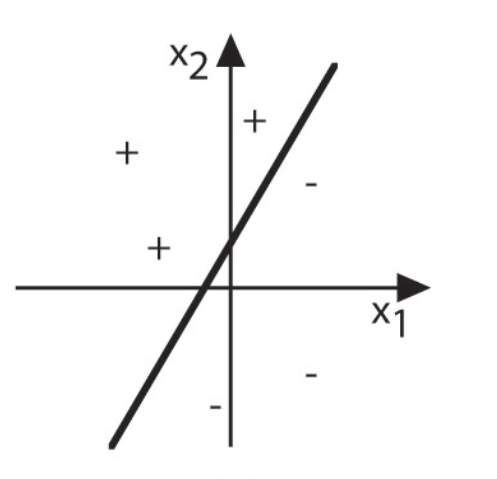
\includegraphics[width=0.50\textwidth]{linearly_separable.png}
\caption{Esempio di dati linearmente separabili tramite una retta.}
\end{figure}

\subsection{Dati non linearmente separabili}

Un insieme di dati è detto \textbf{non linearmente separabile} se non esiste alcun iperpiano in grado di separare perfettamente le classi.

In tali casi, una funzione discriminante lineare non è sufficiente a risolvere il problema di classificazione, rendendo necessaria l’introduzione di modelli non lineari o di trasformazioni dello spazio delle feature.

\begin{figure}[H]
\centering
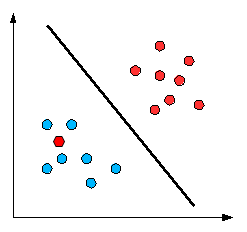
\includegraphics[width=0.6\textwidth]{nonlinearly_separable.png}
\caption{Esempio di dati non linearmente separabili.}
\end{figure}

\section{Linear Discriminant Function}

Una \textbf{funzione discriminante lineare} è una funzione del tipo:
\[
\highlight{
g(x) = w^T x + w_0}
\]

dove:
\begin{itemize}
    \item \( w \in \mathbb{R}^d \) è il vettore dei pesi;
    \item \( w_0 \in \mathbb{R} \) è il termine di bias;
    \item \( g(x) \in \mathbb{R} \) è il valore della funzione discriminante.
\end{itemize}

Essa associa a ogni istanza un valore reale, il cui segno viene utilizzato per effettuare la classificazione.


\subsection{Regola di decisione}

La regola di classificazione basata su una funzione discriminante lineare è:
\[
\highlight{
\text{assegna } x \text{ alla classe }
\begin{cases}
C_1 & \text{se } g(x) \geq 0 \\
C_2 & \text{se } g(x) < 0
\end{cases}}
\]

Il valore assoluto di \( g(x) \) fornisce una misura della distanza dell’istanza dall’iperpiano di separazione.

\subsubsection{Interpretazione geometrica}

\begin{figure}[H]
\centering
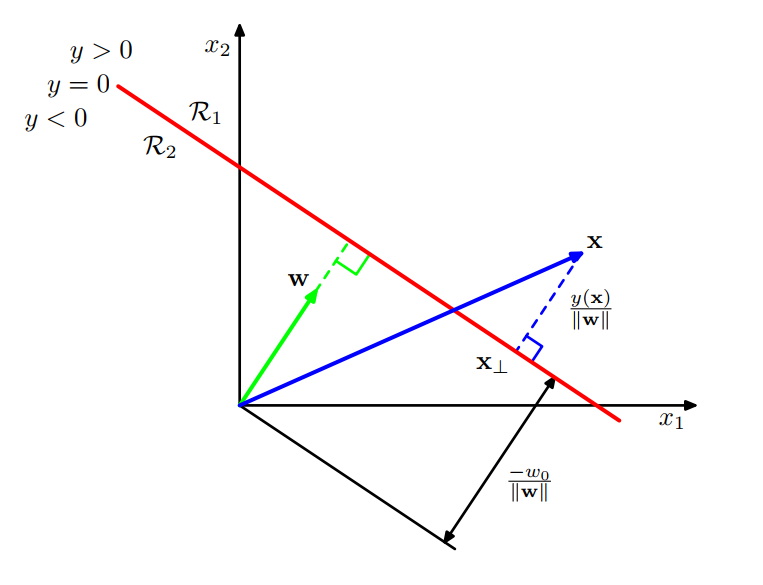
\includegraphics[width=0.7\textwidth]{linear_discriminant_geometry.png}
\caption{Interpretazione geometrica di una funzione discriminante lineare in due dimensioni.}
\end{figure}


Il vettore dei pesi \( w \) è ortogonale all’iperpiano di decisione.
Esso indica la direzione di massima crescita della funzione discriminante.

Nella figura, il vettore \( w \) è rappresentato come una freccia perpendicolare alla retta di separazione.

Dato un punto \( x \), il valore della funzione discriminante \( g(x) \) è proporzionale alla distanza con segno del punto dall’iperpiano.

La distanza geometrica di \( x \) dall’iperpiano è data da:
\[
\frac{g(x)}{\|w\|}
\]

Nella figura, \( x_\perp \) rappresenta la proiezione ortogonale del punto \( x \) sull’iperpiano.

Il termine di bias \( w_0 \) determina la posizione dell’iperpiano rispetto all’origine.
In particolare, la distanza dell’iperpiano dall’origine è:
\[
-\frac{w_0}{\|w\|}
\]

Questo valore controlla la traslazione dell’iperpiano senza modificarne l’orientamento.

\newpage
\section{Learning di funzioni discriminanti lineari}

Nei paragrafi precedenti è stata introdotta la funzione discriminante lineare come strumento per separare due classi mediante un iperpiano nello spazio delle feature.
Resta ora da affrontare il problema fondamentale dell’apprendimento: come determinare i parametri \( w \) e \( w_0 \) a partire da un insieme di dati etichettati.

I \textbf{Linear Discriminant Learning Algorithms} comprendono una famiglia di metodi che apprendono una funzione discriminante lineare a partire da esempi di training.
Tali algoritmi condividono l’obiettivo di costruire una funzione del tipo
\[
g(x) = w^T x + w_0
\]
in grado di separare, nel miglior modo possibile, le istanze appartenenti a classi diverse.

Esistono diversi criteri secondo cui è possibile apprendere una funzione discriminante lineare.
Alcuni algoritmi mirano a separare correttamente i dati, altri a massimizzare una misura di separazione tra le classi, altri ancora a minimizzare un errore globale.

Tra i principali approcci rientrano:
\begin{itemize}
    \item il \textbf{criterio dei minimi quadrati}, che apprende i parametri minimizzando l’errore quadratico tra output desiderato e output del modello;
    \item il \textbf{Perceptron}, che aggiorna iterativamente i pesi correggendo gli errori di classificazione;
    \item il \textbf{Fisher Linear Discriminant}, che massimizza la separazione statistica tra le classi.
    \item il \textbf{Support Vector Machine}, che  trova l'iperpiano ottimale che separa i dati in classi diverse massimizzando il margine tra esse.
\end{itemize}

Nonostante le differenze nei criteri di ottimizzazione, tutti questi metodi producono una funzione discriminante lineare.

\section{Least Squares per la classificazione}

Il criterio dei \textbf{minimi quadrati} rappresenta uno dei metodi più semplici e fondamentali per apprendere una funzione discriminante lineare a partire da un insieme di dati etichettati.
L’idea di base consiste nel trattare il problema di classificazione come un problema di approssimazione funzionale.

\subsection{Definizione del problema}

Si consideri un dataset di training:
\[
\mathcal{D} = \{(x_n, t_n)\}_{n=1}^{N}
\]
dove:
\begin{itemize}
    \item \( x_n \in \mathbb{R}^d \) è il vettore delle feature dell’\(n\)-esimo esempio;
    \item \( t_n \in \mathbb{R} \) è il valore target associato all’esempio.
\end{itemize}

Nel contesto della classificazione binaria, le etichette sono tipicamente codificate come:

\[
t_n \in \{-1, +1\}
\]

Si assume un modello lineare della forma:
\[
y(x) = w^T x + w_0
\]

Introducendo il vettore delle feature esteso:

\[
\tilde{x} = \begin{pmatrix} 1 \\ x \end{pmatrix},
\qquad
\tilde{w} = \begin{pmatrix} w_0 \\ w \end{pmatrix},
\]

il modello può essere riscritto in forma compatta come:

\[
\highlight{
y(x) = \tilde{w}^T \tilde{x}}
\]

\subsection{Funzione di costo}

Il criterio dei minimi quadrati consiste nel minimizzare la somma degli errori quadratici tra l’output del modello e i target desiderati:

\[
\highlight{
E(\tilde{w}) = \frac{1}{2} \sum_{n=1}^{N} \left( y(x_n) - t_n \right)^2}
\]

La funzione di costo misura quanto il modello si discosta dai valori target desiderati sull’insieme di training.
Per ciascun esempio \( x_n \), il termine

\[
\highlight{
\left( y(x_n) - t_n \right)^2}
\]
rappresenta l’errore commesso dal modello su quell’esempio.

La somma degli errori quadratici tiene conto di tutti gli esempi del dataset e penalizza maggiormente gli errori di grande entità.
Minimizzare la funzione di costo equivale quindi a trovare i parametri \( w \) e \( w_0 \) che rendono l’output del modello il più vicino possibile ai target, in media, su tutti i dati di training.


\subsection{Soluzione ottima}

Il minimo della funzione di costo si ottiene imponendo l’annullamento del gradiente:

\[
\nabla E(\tilde{w}) = 0
\]

Da cui si ricavano le \textbf{equazioni normali}:
\[
\tilde{X}^T \tilde{X} \tilde{w} = \tilde{X}^T t
\]

Se la matrice \( \tilde{X}^T \tilde{X} \) è invertibile, la soluzione è:

\[
\highlight{
\tilde{w} = (\tilde{X}^T \tilde{X})^{-1} \tilde{X}^T t}
\]

La soluzione ottima del problema dei minimi quadrati è il vettore dei parametri che minimizza globalmente la funzione di costo.
Poiché la funzione di costo è quadratica nei parametri, essa è convessa e ammette un unico minimo globale.

Questo significa che la soluzione ottenuta risolvendo le equazioni normali è la migliore possibile secondo il criterio dei minimi quadrati, e non dipende dall’inizializzazione dei parametri.

\subsection{Regola di classificazione}

Una volta stimati i parametri \( \tilde{w} \), la classificazione di una nuova istanza \( x \) avviene utilizzando il segno dell’output del modello:

\[
\highlight{
\hat{t} = \text{sign}(y(x)) = \text{sign}(w^T x + w_0)}
\]

Il valore continuo \( y(x) \) può essere interpretato come una misura di confidenza rispetto alla decisione di classificazione.

\subsection{Sensibilità agli outlier}

\begin{figure}[H]
\centering
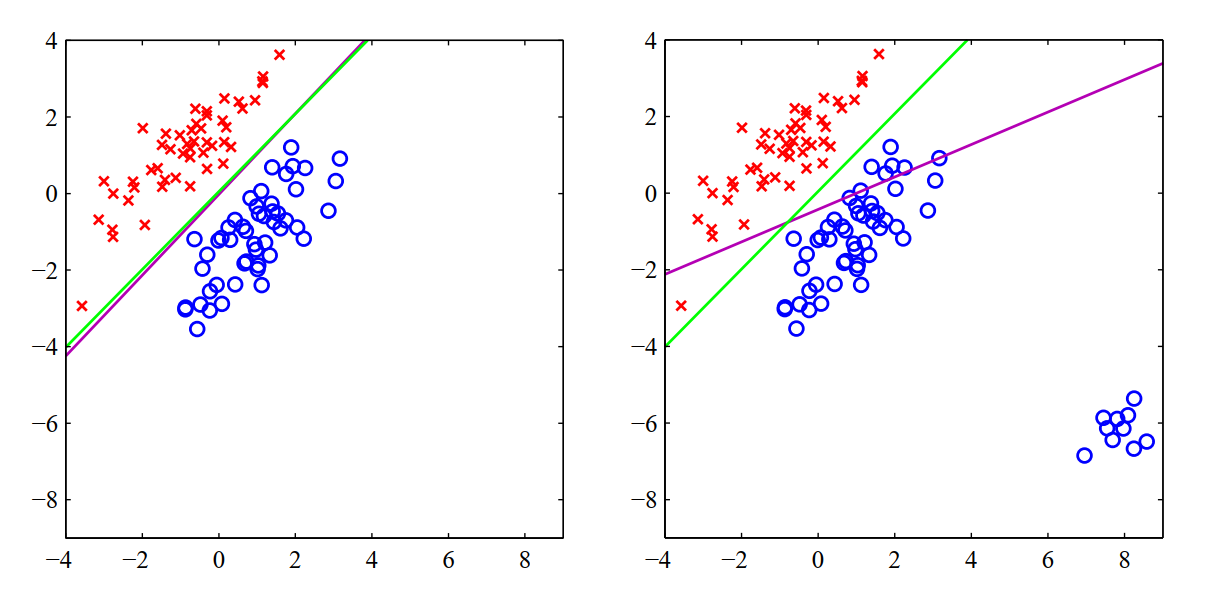
\includegraphics[width=0.9\textwidth]{least_squares_outliers.png}
\caption{\textit{Effetto degli outlier sul metodo dei minimi quadrati. L’aggiunta di pochi punti anomali può modificare significativamente la frontiera di decisione.}}
\end{figure}

La figura illustra l’effetto degli outlier sull’apprendimento di una funzione discriminante lineare tramite il criterio dei minimi quadrati.

Nel pannello di sinistra, le due classi sono ben separate e la funzione discriminante appresa (retta verde) fornisce una separazione ragionevole dei dati.
Nel pannello di destra, l’introduzione di pochi punti anomali (outlier) appartenenti alla classe blu, ma lontani dalla distribuzione principale, provoca una variazione significativa della retta di separazione (retta viola).

Questo comportamento è una conseguenza diretta della funzione di costo dei minimi quadrati:
Poiché l’errore è elevato al quadrato, gli esempi per cui la differenza tra output del modello e target è grande contribuiscono in modo sproporzionato al valore complessivo della funzione di costo.
Di conseguenza, pochi outlier possono dominare l’ottimizzazione e influenzare fortemente la posizione dell’iperpiano appreso.

\subsubsection{NOTA BENE:}
Un metodo di apprendimento si dice \textbf{non robusto agli outlier} quando la presenza di pochi esempi anomali è sufficiente a modificare in modo significativo il modello appreso.

Nel caso del Least Squares, l’algoritmo cerca di ridurre l’errore quadratico complessivo, anche a costo di peggiorare la classificazione della maggioranza dei dati, pur di adattarsi ai punti anomali.
Questo limite rende il criterio dei minimi quadrati poco adatto ai problemi di classificazione, in cui l’obiettivo principale è la corretta separazione delle classi piuttosto che l’approssimazione numerica dei target.

Tale osservazione motiva l’introduzione di algoritmi alternativi, come il perceptron o i metodi basati su funzioni di costo non quadratiche, più robusti alla presenza di outlier.

\section{Perceptron}

Il \textbf{Perceptron} è uno dei più semplici algoritmi di apprendimento supervisionato per la classificazione binaria.
Esso apprende una funzione discriminante lineare a partire da esempi etichettati, aggiornando iterativamente i parametri del modello in base agli errori di classificazione.

Il Perceptron può essere interpretato sia come un algoritmo di apprendimento per funzioni discriminanti lineari, sia come un modello elementare di neurone artificiale.

\subsection{Definizione del problema}

Si consideri un insieme di dati di training:
\[
\mathcal{D} = \{(x_n, t_n)\}_{n=1}^{N}
\]
dove:
\begin{itemize}
    \item \( x_n \in \mathbb{R}^d \) è il vettore delle feature dell’\(n\)-esimo esempio;
    \item \( t_n \in \{-1, +1\} \) è l’etichetta di classe associata.
\end{itemize}

L’obiettivo è apprendere una funzione:
\[
f : \mathbb{R}^d \rightarrow \{-1, +1\}
\]
che assegni correttamente un’etichetta di classe a nuove istanze non osservate.

\subsection{Modello del Perceptron}

Il Perceptron utilizza un modello lineare della forma:
\[
g(x) = w^T x + w_0
\]

L’output del classificatore è ottenuto applicando una funzione di soglia:

\[
\highlight{
o(x) =
\begin{cases}
+1 & \text{se } g(x) > 0 \\
-1 & \text{altrimenti}
\end{cases}
=
\text{sign}(w^T x + w_0)}
\]

La funzione di soglia separa lo spazio delle feature in due regioni distinte, corrispondenti alle due classi.
Il valore assoluto di \( g(x) \) indica quanto il punto si trovi lontano dall’iperpiano di decisione, ma non influisce direttamente sulla decisione finale.

Questo comportamento distingue il Perceptron da modelli probabilistici, nei quali l’output rappresenta una probabilità.

\subsection{Perceptron Learning Rule}

L’apprendimento nel Perceptron avviene in modo iterativo, aggiornando i pesi solo quando un esempio di training viene classificato in modo errato.

Dato un esempio \( (x_n, t_n) \), con \( t_n \in \{-1, +1\} \), il modello produce un output:

\[
\highlight{
o(x_n) = \text{sign}(w^T x_n + w_0).}
\]

Se \( o(x_n) = t_n \), l’esempio è classificato correttamente e non viene effettuato alcun aggiornamento.
Se invece \( o(x_n) \neq t_n \), i parametri vengono aggiornati secondo la seguente regola.


In presenza di errore di classificazione, i pesi vengono aggiornati come:

\[
w \leftarrow w + \eta \, t_n \, x_n
\]
\[
w_0 \leftarrow w_0 + \eta \, t_n 
\]

dove \( \eta > 0 \) è il tasso di apprendimento.

L’aggiornamento dei pesi modifica l’iperpiano di decisione in modo da ridurre l’errore commesso sull’esempio corrente.

In particolare:
\begin{itemize}
    \item se un esempio positivo viene classificato come negativo, il termine \( t_n x_n \) spinge l’iperpiano verso l’esempio;
    \item se un esempio negativo viene classificato come positivo, l’aggiornamento avviene nella direzione opposta.
\end{itemize}

In questo modo, l’iperpiano viene progressivamente adattato per separare correttamente i dati.

\subsubsection*{Forma compatta}

La regola di aggiornamento del Perceptron può essere scritta in forma compatta come:

\[
\highlight{
w \leftarrow w + \eta \, t_n \, x_n
\quad \text{se } t_n (w^T x_n + w_0) \leq 0.}
\]

Questa espressione evidenzia che l’aggiornamento avviene esclusivamente in presenza di errore.

\newpage
\subsection{Algoritmo del Perceptron}

\begin{pseudocode}
Input:
    Training set D = {(x_n, t_n)}, t_n in {-1, +1}
    Learning rate eta > 0

Initialize:
    w = 0
    w0 = 0

Repeat until convergence:
    for each (x_n, t_n) in D:
        if t_n * (w^T x_n + w0) <= 0 then
            w  <- w  + eta * t_n * x_n
            w0 <- w0 + eta * t_n
        end if
    end for
\end{pseudocode}

L’algoritmo del Perceptron procede iterativamente scorrendo il dataset di training. 
Per ciascun esempio, viene verificata la correttezza della classificazione.

Se un esempio è classificato correttamente, i parametri restano invariati.
In caso contrario, i pesi e il bias vengono aggiornati per correggere l’errore.
L’algoritmo termina quando un intero passaggio sui dati non produce aggiornamenti.

\subsubsection{Esempio di applicazione}

Si consideri un semplice dataset bidimensionale con target binari:

\[
\mathcal{D} = \{(x_1, t_1), (x_2, t_2), (x_3, t_3)\}
\]
con:
\[
x_1 = (1,1), \quad t_1 = +1
\]
\[
x_2 = (2,0), \quad t_2 = +1
\]
\[
x_3 = (-1,-1), \quad t_3 = -1
\]

Si inizializzano i parametri:
\[
w = (0,0), \qquad w_0 = 0
\]
e si assume \( \eta = 1 \).

Per il primo esempio \( x_1 = (1,1) \):
\[
g(x_1) = w^T x_1 + w_0 = 0
\]

Poiché:
\[
t_1 g(x_1) = 0 \leq 0,
\]
l’esempio è considerato errato e si applica l’aggiornamento:
\[
w \leftarrow (0,0) + 1 \cdot (+1) \cdot (1,1) = (1,1)
\]
\[
w_0 \leftarrow 0 + 1 \cdot (+1) = 1
\]

Per \( x_2 = (2,0) \):
\[
g(x_2) = (1,1)^T (2,0) + 1 = 3
\]

Poiché:
\[
t_2 g(x_2) = (+1)\cdot 3 > 0,
\]
l’esempio è classificato correttamente e non viene effettuato alcun aggiornamento.

Per \( x_3 = (-1,-1) \):
\[
g(x_3) = (1,1)^T (-1,-1) + 1 = -1
\]

Poiché:
\[
t_3 g(x_3) = (-1)\cdot (-1) > 0,
\]
anche questo esempio è classificato correttamente.

Al termine del primo ciclo sui dati, non si verificano ulteriori errori.
L’iperpiano appreso è quindi:
\[
w^T x + w_0 = 0 \quad \Rightarrow \quad x_1 + x_2 + 1 = 0
\]

Questo iperpiano separa correttamente le due classi del dataset.

\subsubsection{Visualizzazione dell’algoritmo del Perceptron}

\begin{figure}[H]
\centering
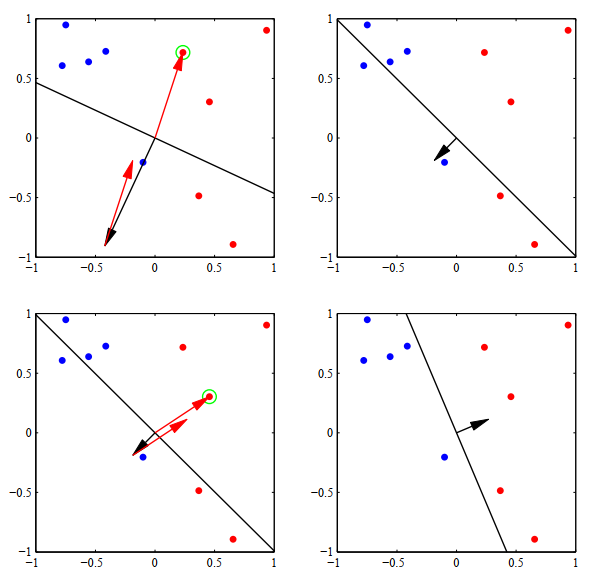
\includegraphics[width=0.85\textwidth]{perceptron_training_process.png}
\caption{\textit{Evoluzione dell’iperpiano di decisione durante l’apprendimento del Perceptron. Ogni pannello rappresenta un aggiornamento successivo dei pesi in risposta a un errore di classificazione.}}
\end{figure}

La figura mostra il comportamento dell’algoritmo del Perceptron durante il processo di apprendimento su un dataset bidimensionale.

In ciascun pannello è rappresentato l’iperpiano di decisione corrente, insieme agli esempi di training appartenenti alle due classi.
Le frecce indicano la direzione dell’aggiornamento dei pesi quando viene incontrato un esempio classificato erroneamente.
Quando un esempio viene classificato in modo errato, il Perceptron modifica i parametri del modello secondo la regola:
\[
w \leftarrow w + \eta\, t_n\, x_n
\]

Questo aggiornamento sposta l’iperpiano nella direzione dell’esempio mal classificato se \( t_n = +1 \), o nella direzione opposta se \( t_n = -1 \).
Nella figura, i punti cerchiati evidenziano gli esempi che causano l’aggiornamento dei pesi.

Dal punto di vista geometrico, ogni aggiornamento ruota e trasla l’iperpiano di decisione nel tentativo di ridurre il numero di errori di classificazione.

Il Perceptron non ottimizza una funzione di costo globale, ma corregge localmente l’errore commesso sull’esempio corrente.
Di conseguenza, la traiettoria seguita dall’iperpiano dipende dall’ordine con cui vengono presentati i dati di training.

\subsection{Interpretazione neurale}

Il perceptron è la forma più semplice di rete neurale: consiste in un singolo neurone artificiale che riceve input pesati, li somma, applica una funzione di attivazione (tipicamente a gradino) e produce un output binario per classificare linearmente i dati.
Storicamente è stato il primo modello di rete neurale (proposto da Rosenblatt nel 1958) e ha posto le basi concettuali per le reti neurali moderne. La sua limitazione principale è che può risolvere solo problemi linearmente separabili - per questo motivo le reti neurali si sono evolute in architetture multi-strato (multilayer perceptron o MLP) capaci di apprendere relazioni non lineari grazie ai neuroni nascosti e alla retropropagazione dell'errore.

\begin{figure}[H]
\centering
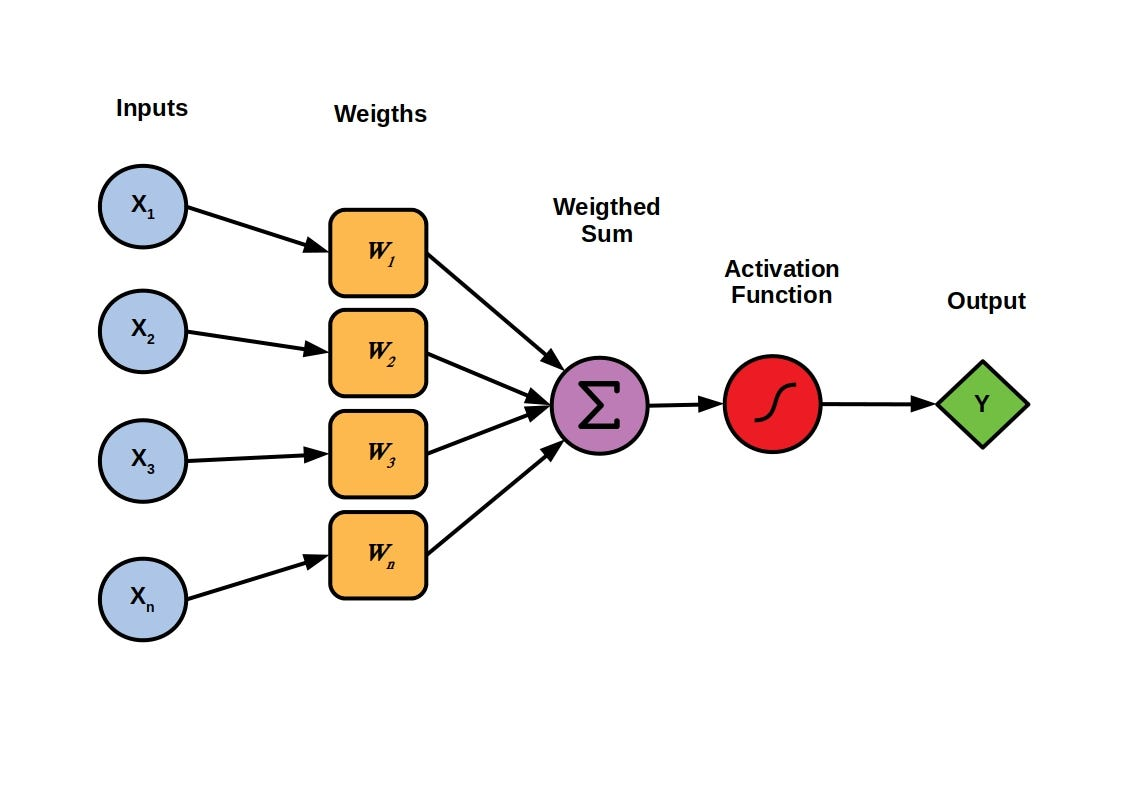
\includegraphics[width=0.85\textwidth]{perceptron.jpg}
\caption{Visualizzazion grafica del Perceptron come neurone artificiale.}
\end{figure}

Nell'immagine vediamo come ciascun input \( x_i \) è associato a un peso \( w_i \), mentre il termine di bias è modellato tramite un input costante \( x_0 = 1 \) con peso \( w_0 \).

Il neurone calcola una combinazione lineare degli input:
\[
\sum_{i=0}^{d} w_i x_i
\]
e applica una funzione di attivazione a soglia che restituisce l’etichetta di classe.

\section{Fisher's Linear Discriminant}

Il \textbf{Fisher’s Linear Discriminant} è un metodo di classificazione lineare basato su un criterio statistico.
A differenza del Perceptron e del Least Squares, che si basano rispettivamente sugli errori di classificazione e sull’errore quadratico, il metodo di Fisher mira a massimizzare la separazione tra le classi in termini di distribuzione dei dati.

\subsubsection{Impostazione del problema}

Si consideri un problema di classificazione binaria con due classi:
\[
\mathcal{C}_1 \quad \text{e} \quad \mathcal{C}_2
\]

Ciascun esempio \( x \in \mathbb{R}^d \) viene proiettato su una retta mediante una funzione lineare:

\[
\highlight{
y = w^T x}
\]

L’obiettivo è determinare il vettore \( w \) tale che, dopo la proiezione, le due classi risultino il più possibile separate.

L’idea centrale del Fisher’s Linear Discriminant consiste nel trovare una direzione di proiezione che:
\begin{itemize}
    \item massimizzi la distanza tra le medie delle classi proiettate;
    \item minimizzi la dispersione interna a ciascuna classe.
\end{itemize}

In questo modo, le classi risultano ben separate lungo la direzione di proiezione scelta.

\subsection{Medie delle classi}

Siano:
\[
\mu_1 = \frac{1}{N_1} \sum_{x \in \mathcal{C}_1} x,
\qquad
\mu_2 = \frac{1}{N_2} \sum_{x \in \mathcal{C}_2} x
\]

le medie dei dati appartenenti alle due classi nello spazio originale.
Dopo la proiezione sulla direzione \( w \), le medie diventano:
\[
m_1 = w^T \mu_1,
\qquad
m_2 = w^T \mu_2
\]

\subsection{Varianza intra-classe}

La dispersione dei dati di ciascuna classe dopo la proiezione è misurata dalla varianza:
\[
s_i^2 = \sum_{x \in \mathcal{C}_i} (w^T x - m_i)^2, \quad i = 1,2
\]

La varianza totale intra-classe è definita come:
\[
s_w^2 = s_1^2 + s_2^2
\]

\subsection{Criterio di Fisher}

Il criterio di Fisher è definito come il rapporto tra la distanza quadratica tra le medie proiettate e la varianza intra-classe:

\[
\highlight{
J(w) = \frac{(m_1 - m_2)^2}{s_w^2}}
\]

Il problema di apprendimento consiste nel trovare il vettore \( w \) che massimizza tale criterio.

\subsubsection{Forma matriciale}

Introducendo le matrici di dispersione intra-classe:
\[
S_i = \sum_{x \in \mathcal{C}_i} (x - \mu_i)(x - \mu_i)^T,
\quad i = 1,2
\]

e la matrice di dispersione totale:
\[
S_W = S_1 + S_2,
\]

il criterio di Fisher può essere riscritto come:

\[
\highlight{
J(w) = \frac{w^T (\mu_1 - \mu_2)(\mu_1 - \mu_2)^T w}{w^T S_W w}}
\]

\subsubsection{Interpretazione geometrica del criterio di Fisher}

\begin{figure}[H]
\centering
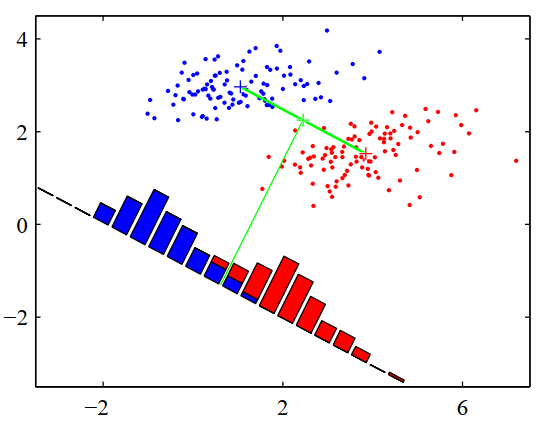
\includegraphics[width=0.85\textwidth]{fisher_mean_difference.png}
\caption{\textit{Proiezione lungo la direzione della differenza delle medie. La dispersione intra-classe non è considerata.}}
\end{figure}

Questa prima figura mostra una proiezione dei dati lungo la direzione che unisce le medie delle due classi.
Questa scelta massimizza la distanza tra le medie proiettate, ma non tiene conto della dispersione interna delle classi.

Se una classe presenta un’elevata varianza lungo tale direzione, le distribuzioni proiettate possono sovrapporsi significativamente, riducendo la capacità discriminante.

\begin{figure}[H]
\centering
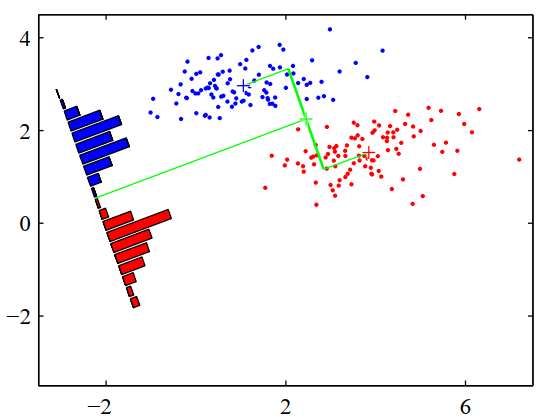
\includegraphics[width=0.85\textwidth]{fisher_optimal_projection.png}
\caption{\textit{Proiezione secondo il Fisher Linear Discriminant. La dispersione intra-classe viene tenuta in conto.}}
\end{figure}

Questa seconda figura invece illustra la soluzione del Fisher Linear Discriminant.
L’introduzione della matrice di dispersione intra-classe \( S_W \) consente di penalizzare le direzioni caratterizzate da elevata varianza.

La direzione di proiezione risultante massimizza la separazione tra le classi tenendo conto sia della distanza tra le medie sia della compattezza delle distribuzioni.

\subsubsection{Soluzione ottima}

Massimizzando il criterio di Fisher, si ottiene che il vettore ottimo è proporzionale a:

\[
\highlight{
w \propto S_W^{-1} (\mu_1 - \mu_2)}
\]

Questa direzione massimizza la separazione tra le classi dopo la proiezione.

\subsubsection{Regola di classificazione}

Una volta determinata la direzione \( w \), un nuovo esempio \( x \) viene classificato proiettandolo su \( w \) e confrontando il risultato con una soglia \( \theta \):
\[
\text{classe}(x) =
\begin{cases}
\mathcal{C}_1 & \text{se } w^T x \ge \theta \\
\mathcal{C}_2 & \text{altrimenti}
\end{cases}
\]

La soglia può essere scelta, ad esempio, come il punto medio tra le medie proiettate delle due classi.

\section{Support Vector Machine}

Le \textbf{Support Vector Machine (SVM)} sono una classe di algoritmi di apprendimento supervisionato per la classificazione (e regressione), basati sulla costruzione di un iperpiano di decisione ottimale.

Come nel caso del Perceptron e del Fisher Linear Discriminant, anche le SVM costruiscono una funzione discriminante lineare della forma:

\[
g(x) = w^T x + b
\]

Tuttavia, mentre il Perceptron si limita a correggere gli errori di classificazione e il metodo di Fisher massimizza una misura statistica di separazione, le SVM introducono un criterio geometrico esplicito basato sul margine.

Il margine di un iperpiano di decisione è definito come la distanza minima tra l’iperpiano stesso e i punti del dataset più vicini ad esso.

L’idea alla base delle SVM è che un iperpiano con margine massimo presenti migliori proprietà di generalizzazione, risultando meno sensibile al rumore e alle variazioni nei dati di training.


\subsection{Formulazione formale}

Si consideri un problema di classificazione binaria con un dataset di training
\[
\mathcal{D} = \{(x_i, y_i)\}_{i=1}^{N},
\]
dove \( x_i \in \mathbb{R}^d \) rappresenta il vettore delle feature e \( y_i \in \{-1,+1\} \) l’etichetta di classe.

L’obiettivo delle Support Vector Machine è apprendere una funzione discriminante lineare della forma
\[
f(x) = w^T x + b,
\]
in grado di separare correttamente le due classi mediante un iperpiano di decisione definito dall’equazione
\[
w^T x + b = 0.
\]

Un punto \( x \) viene classificato in base al segno della funzione discriminante:
\[
\text{classe}(x) = \text{sign}(w^T x + b).
\]

La distanza geometrica di un punto \( x_i \) dall’iperpiano di decisione è data da
\[
\frac{|w^T x_i + b|}{\|w\|}.
\]
Il margine di classificazione è definito come la distanza minima tra l’iperpiano e i punti del dataset.
Le Support Vector Machine cercano l’iperpiano che massimizza tale margine.

Nel caso di dati linearmente separabili, è possibile imporre i vincoli di separazione
\[
y_i (w^T x_i + b) \geq 1, \quad \forall i = 1,\dots,N.
\]
Questa scelta fissa la scala dei parametri e consente di definire in modo univoco il margine geometrico, che risulta pari a \( \frac{2}{\|w\|} \).

Il problema di apprendimento di una SVM hard-margin può quindi essere formulato come il seguente problema di ottimizzazione convessa:
\[
\begin{aligned}
\min_{w,b} \quad & \frac{1}{2}\|w\|^2 \\
\text{soggetto a} \quad & y_i (w^T x_i + b) \geq 1, \quad \forall i.
\end{aligned}
\]

La funzione obiettivo consiste nella minimizzazione della norma del vettore dei pesi.
Poiché il margine è inversamente proporzionale a \( \|w\| \), minimizzare \( \|w\|^2 \) equivale a massimizzare il margine di separazione tra le classi.

I punti del dataset che soddisfano il vincolo con uguaglianza,
\[
y_i (w^T x_i + b) = 1,
\]
sono detti \textbf{support vectors}.
Essi sono gli unici esempi che contribuiscono direttamente alla determinazione dell’iperpiano ottimale, mentre tutti gli altri punti non influenzano la soluzione finale una volta fissato il margine.

\subsection*{Interpretazione geometrica del margine}

\begin{figure}[H]
\centering
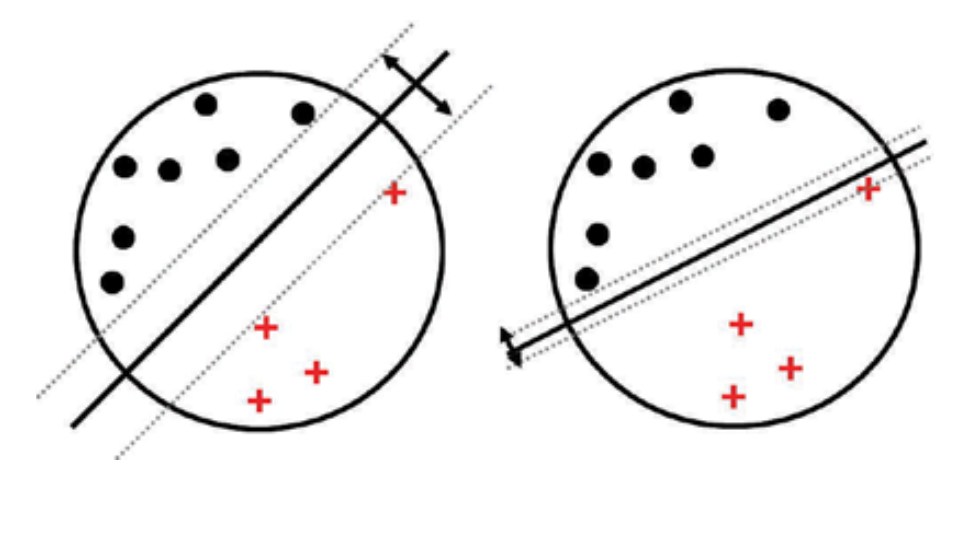
\includegraphics[width=0.9\textwidth]{svm_maximum_margin.png}
\caption{\textit{Confronto tra diversi iperpiani separatori: a sinistra un iperpiano con margine ridotto, a destra l’iperpiano a margine massimo individuato dalle SVM.}}
\end{figure}

La figura mostra il principio fondamentale alla base delle Support Vector Machine.
Nel pannello di sinistra è rappresentato un iperpiano che separa correttamente le due classi, ma presenta un margine ridotto.
Piccole variazioni nei dati o la presenza di rumore potrebbero compromettere la corretta classificazione.

Nel pannello di destra è invece mostrato l’iperpiano a margine massimo.
Questo iperpiano massimizza la distanza tra le due classi, risultando più stabile e robusto rispetto a perturbazioni nei dati.

\subsection{Soft-Margin Support Vector Machine}

Nel caso reale, i dati di training non sono quasi mai perfettamente linearmente separabili.
La presenza di rumore, outlier o sovrapposizione tra le classi rende impossibile soddisfare rigidamente i vincoli dell’hard-margin SVM.
Per questo motivo, le Support Vector Machine introducono il concetto di \textbf{soft margin}, che consente alcune violazioni controllate dei vincoli di separazione mantenendo il principio del margine massimo.

Nel soft-margin SVM vengono introdotte delle variabili di slack \( \xi_i \geq 0 \), una per ciascun esempio di training, che misurano il grado di violazione del vincolo di separazione.
I vincoli diventano quindi:
\[
y_i (w^T x_i + b) \geq 1 - \xi_i, \quad \forall i = 1,\dots,N.
\]

Il significato delle variabili di slack è il seguente:
un esempio con \( \xi_i = 0 \) è correttamente classificato e si trova al di fuori del margine o esattamente sul margine;
un esempio con \( 0 < \xi_i < 1 \) è correttamente classificato ma si trova all’interno del margine;
un esempio con \( \xi_i \geq 1 \) è classificato erroneamente.

Il problema di apprendimento del soft-margin SVM può essere formulato come il seguente problema di ottimizzazione convessa:
\[
\begin{aligned}
\min_{w,b,\xi} \quad & \frac{1}{2}\|w\|^2 + C \sum_{i=1}^{N} \xi_i \\
\text{soggetto a} \quad & y_i (w^T x_i + b) \geq 1 - \xi_i, \quad \forall i, \\
& \xi_i \geq 0, \quad \forall i.
\end{aligned}
\]

La funzione obiettivo è composta da due termini in competizione tra loro.
Il termine \( \frac{1}{2}\|w\|^2 \) tende a massimizzare il margine di separazione tra le classi, mentre il termine \( C \sum_i \xi_i \) penalizza le violazioni dei vincoli di separazione.
Il parametro \( C > 0 \) controlla il compromesso tra l’ampiezza del margine e l’accuratezza sui dati di training.

Valori elevati di \( C \) assegnano un peso maggiore agli errori di classificazione, portando a un margine più stretto ma a un numero ridotto di violazioni.
Al contrario, valori piccoli di \( C \) consentono margini più ampi, tollerando un numero maggiore di errori sul training set, con potenziali benefici in termini di generalizzazione.

Anche nel caso soft-margin, i support vectors sono costituiti dagli esempi per cui il vincolo è attivo, ovvero quelli che soddisfano:
\[
y_i (w^T x_i + b) \leq 1.
\]
Questi includono sia i punti sul margine sia quelli che si trovano all’interno del margine o lo violano, e sono gli unici esempi che contribuiscono direttamente alla definizione dell’iperpiano ottimale.

Il soft-margin SVM generalizza l’hard-margin SVM, che può essere visto come un caso particolare ottenuto per \( C \to \infty \).
Grazie all’introduzione delle variabili di slack, le Support Vector Machine risultano applicabili a problemi reali caratterizzati da rumore e non perfetta separabilità delle classi.

\subsection{Interpretazione geometrica}
\begin{figure}[H]
\centering
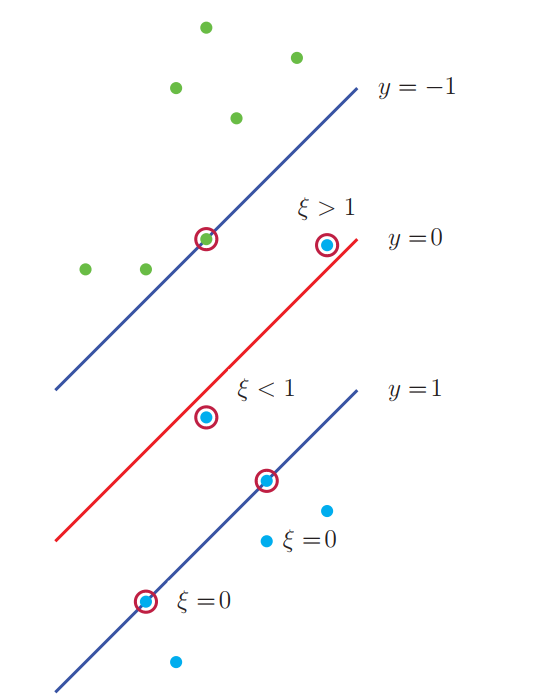
\includegraphics[width=0.75\textwidth]{soft_margin_slack.png}
\caption{\textit{Interpretazione geometrica delle variabili di slack nel soft-margin SVM.}}
\end{figure}

La figura illustra il significato geometrico delle variabili di slack \( \xi_i \) nel contesto del soft-margin SVM.
Le tre rette rappresentano, rispettivamente, l’iperpiano di decisione \( w^T x + b = 0 \) e i due margini \( w^T x + b = \pm 1 \).

I punti appartenenti alle due classi sono distribuiti nello spazio delle feature e la loro posizione rispetto ai margini determina il valore della variabile di slack associata.
Un punto per cui \( 0 < \xi_i \leq 1 \) si trova all’interno del margine, ma sul lato corretto dell’iperpiano di decisione.
In questo caso il punto è correttamente classificato, ma contribuisce comunque alla penalizzazione nella funzione obiettivo.

Infine, un punto per cui \( \xi_i > 1 \) si trova sul lato sbagliato dell’iperpiano di decisione ed è quindi classificato erroneamente.
In particolare, quando \( \xi_i = 1 \) il punto giace esattamente sull’iperpiano di decisione, mentre per \( \xi_i > 1 \) la classificazione risulta errata.
La figura evidenzia come il soft-margin SVM consenta di tollerare violazioni dei vincoli di separazione, penalizzandole in modo controllato attraverso le variabili di slack, anziché imporre una separazione rigida come nel caso dell’hard-margin.

\subsection{Basis Functions e separazione non lineare}

Nei casi reali, i dati non sono spesso linearmente separabili nello spazio originale delle feature.
In queste situazioni, una funzione discriminante lineare non è sufficiente a descrivere una frontiera di decisione efficace.
L’idea alla base dell’uso delle \textbf{basis functions} consiste nel trasformare le istanze originali in uno spazio delle feature di dimensione maggiore, nel quale una separazione lineare diventa possibile.

Formalmente, si introduce una mappa non lineare:
\[
\phi : \mathbb{R}^d \rightarrow \mathbb{R}^M,
\]
che associa a ciascun input \( x \) un nuovo vettore di feature \( \phi(x) \).
La funzione discriminante assume quindi la forma:
\[
f(x) = w^T \phi(x) + b.
\]

In questo nuovo spazio delle feature, la funzione di decisione rimane lineare rispetto ai parametri \( w \), ma risulta non lineare rispetto alle variabili originali.
Questo consente di modellare frontiere di decisione complesse nello spazio di input.

Un primo esempio di basis functions è dato dalle \textbf{polynomial basis functions}.
Nel caso monodimensionale, una trasformazione polinomiale di grado due può essere scritta come:
\[
\phi(x) = (1, x, x^2).
\]
In questo modo, una funzione lineare nello spazio delle feature corrisponde a una funzione quadratica nello spazio originale.

Un secondo esempio molto utilizzato è rappresentato dalle \textbf{Gaussian basis functions}, definite come:
\[
\phi_j(x) = \exp\left( -\frac{\|x - \mu_j\|^2}{2\sigma^2} \right),
\]
dove \( \mu_j \) rappresenta il centro della funzione e \( \sigma \) ne controlla l’ampiezza.
Queste funzioni consentono di modellare regioni locali nello spazio delle feature e risultano particolarmente efficaci in presenza di distribuzioni complesse.

Un’ulteriore classe di trasformazioni è data dalle \textbf{sigmoidal basis functions}, definite come:
\[
\phi_j(x) = \tanh(a_j^T x + b_j),
\]
che introducono una non linearità simile a quella dei neuroni artificiali.

L’uso esplicito delle basis functions presenta tuttavia un limite pratico: la dimensione dello spazio delle feature può diventare molto elevata o addirittura infinita.
Le Support Vector Machine superano questo problema attraverso il \textbf{kernel trick}, che consente di calcolare prodotti scalari nello spazio delle feature senza esplicitare la mappa \( \phi(x) \).

In questo modo, le SVM riescono a costruire classificatori non lineari mantenendo una formulazione computazionalmente efficiente e una solida base teorica.

\section{RIEPILOGO}

\begin{tcolorbox}[
    colback=green!10,
    colframe=green!50!black,
    title=Support Vector Machine -- Concetti chiave
]

Le \textbf{Support Vector Machine (SVM)} sono classificatori supervisionati basati sulla ricerca di un iperpiano di decisione che massimizza il \textbf{margine} tra le classi, migliorando la capacità di generalizzazione.

\medskip

\textbf{Hard-margin SVM}  
Nel caso di dati linearmente separabili, il problema consiste nel minimizzare:
\[
\frac{1}{2}\|w\|^2
\]
soggetto ai vincoli:
\[
y_i(w^T x_i + b) \geq 1.
\]
I punti che soddisfano il vincolo con uguaglianza sono detti \textbf{support vectors} e determinano univocamente l’iperpiano ottimale.

\medskip

\textbf{Soft-margin SVM}  
Per dati non perfettamente separabili, vengono introdotte le variabili di slack \( \xi_i \geq 0 \) e il problema diventa:
\[
\min_{w,b,\xi} \; \frac{1}{2}\|w\|^2 + C \sum_i \xi_i,
\quad
y_i(w^T x_i + b) \geq 1 - \xi_i.
\]
Il parametro \( C \) regola il compromesso tra ampiezza del margine e penalizzazione degli errori.

\medskip

\textbf{Interpretazione delle variabili di slack}
\begin{itemize}
    \item \( \xi_i = 0 \): punto correttamente classificato e fuori dal margine;
    \item \( 0 < \xi_i \leq 1 \): punto dentro il margine ma sul lato corretto;
    \item \( \xi_i > 1 \): punto misclassificato.
\end{itemize}

\medskip

\textbf{Separazione non lineare e basis functions}  
Quando i dati non sono linearmente separabili nello spazio originale, è possibile applicare una trasformazione non lineare:
\[
\phi : \mathbb{R}^d \rightarrow \mathbb{R}^M,
\quad
f(x) = w^T \phi(x) + b.
\]
Esempi di basis functions includono trasformazioni polinomiali, gaussiane e sigmoidali.

\medskip

In sintesi, le SVM combinano un criterio geometrico solido, una formulazione di ottimizzazione convessa e la possibilità di estendere il modello a separazioni non lineari, rendendole uno dei metodi di riferimento nel machine learning classico.

\end{tcolorbox}

\newpage
\chapter{Linear Models for Regression}

L’obiettivo della regressione è apprendere una funzione

\[
\highlight{
f : \mathcal{X} \subseteq \mathbb{R}^d \rightarrow \mathbb{R}}
\]

a partire da un insieme di dati

\[
\highlight{
\mathcal{D} = \{(x_n, t_n)\}_{n=1}^N,}
\]

dove $x_n$ rappresenta un vettore di input e $t_n$ il corrispondente valore target reale. I modelli lineari per la regressione assumono che l’output possa essere espresso come combinazione lineare di parametri, eventualmente applicata a trasformazioni non lineari degli input.

\section{Modelli lineari per funzioni lineari}

Nel caso più semplice, il modello è lineare rispetto alle variabili di input:

\[
\highlight{
y(x; w) = w_0 + w_1 x_1 + \dots + w_d x_d = w^T x,}
\]

dove il vettore degli input è esteso con un termine costante
\[
x = \begin{bmatrix} 1 & x_1 & \dots & x_d \end{bmatrix}^T,
\]
e il vettore dei parametri è
\[
w = \begin{bmatrix} w_0 & w_1 & \dots & w_d \end{bmatrix}^T.
\]
Questo modello consente, ad esempio, di approssimare una retta nel caso bidimensionale, come nel classico problema di \emph{line fitting}.

Nel caso di una singola variabile di input, il modello lineare assume la forma
\[
\highlight{
y(x; w) = w_0 + w_1 x_1,}
\]
che corrisponde geometricamente a una retta nel piano. Come illustrato in Figura~\ref{fig:linear_fit}, i dati osservati non giacciono esattamente sulla retta a causa della presenza di rumore sulle misure. Il problema della regressione consiste quindi nel determinare i parametri $w_0$ e $w_1$ tali da approssimare nel modo migliore possibile i valori target.

\begin{figure}[H]
    \centering
    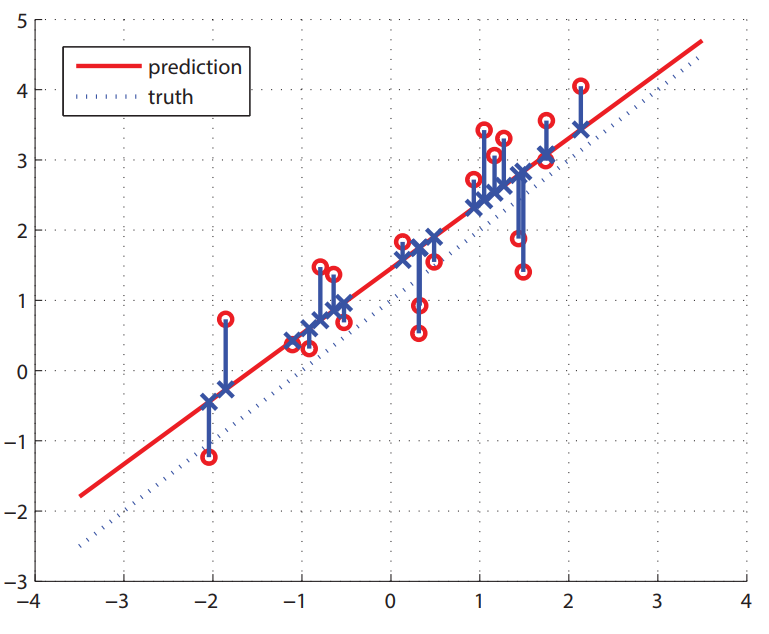
\includegraphics[width=0.65\textwidth]{linear_regression_2d.png}
    \caption{Esempio di regressione lineare bidimensionale. I punti blu rappresentano i valori target osservati, affetti da rumore, mentre la retta rossa corrisponde alla funzione di predizione $y(x;w)=w_0+w_1x_1$ appresa dal modello. I segmenti verticali indicano i residui, ovvero gli errori $t_n - y(x_n;w)$ che vengono minimizzati nel criterio dei minimi quadrati.}
    \label{fig:linear_fit}
\end{figure}

Gli scarti verticali tra i punti osservati e la retta di predizione rappresentano i residui del modello. La stima dei parametri tramite il metodo dei minimi quadrati equivale a minimizzare la somma dei quadrati di tali residui, fornendo la soluzione ottima in senso statistico sotto l’ipotesi di rumore gaussiano.


\section{Modelli lineari con basis functions}

Per aumentare la flessibilità del modello senza rinunciare alla linearità nei parametri, si introducono le \emph{basis functions}. Il modello assume la forma

\[
\highlight{
y(x; w) = \sum_{j=0}^{M} w_j \phi_j(x) = w^T \phi(x),}
\]

dove $\phi_j(x)$ sono funzioni (in generale non lineari) degli input, con $\phi_0(x) = 1$. Nonostante la possibile non linearità rispetto a $x$, il modello rimane lineare rispetto ai parametri $w$.

Un caso particolarmente rilevante di modelli lineari con basis functions è rappresentato dall’uso di polinomi. In questo contesto, le funzioni base sono definite come

\[
\highlight{
\phi_j(x) = x^j,}
\]

e il modello assume la forma

\[
\highlight{
y(x;w) = \sum_{j=0}^{M} w_j x^j.}
\]

\begin{figure}[h!]
    \centering
    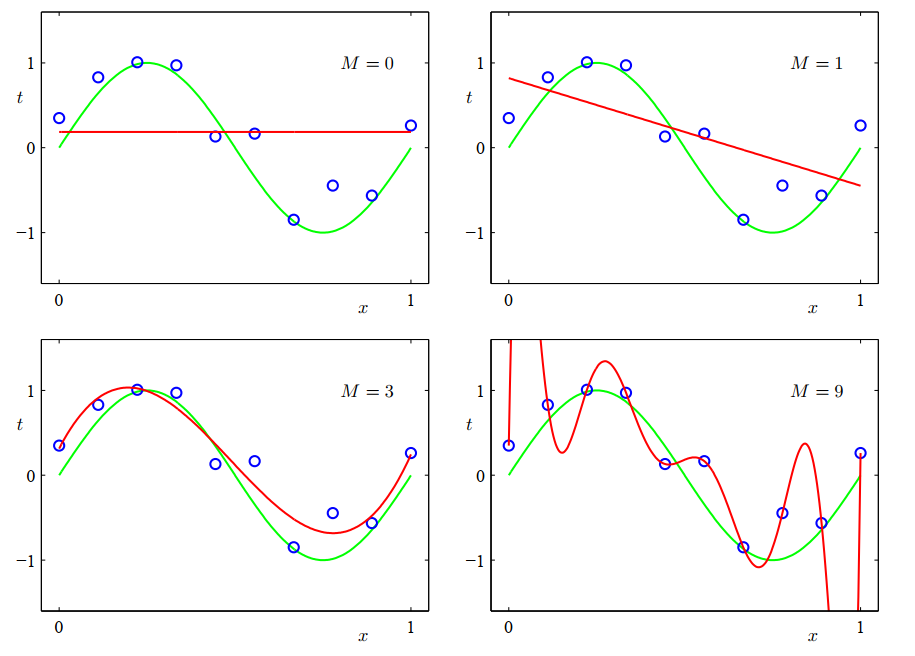
\includegraphics[width=0.9\textwidth]{polinomial_curve_fitting.png}
    \caption{Esempio di regressione mediante basis functions polinomiali di diverso grado $M$. I punti blu rappresentano i dati osservati, la curva verde indica la funzione target sottostante, mentre la curva rossa corrisponde alla funzione appresa dal modello. All’aumentare del grado del polinomio cresce la flessibilità del modello, passando da situazioni di underfitting ($M=0,1$) a una buona approssimazione ($M=3$), fino a fenomeni di overfitting ($M=9$).}
    \label{fig:polynomial_basis}
\end{figure}

La Figura~\ref{fig:polynomial_basis} mostra come la scelta del grado $M$ influenzi in modo critico il comportamento del modello. Per valori piccoli di $M$, il modello risulta eccessivamente rigido e non è in grado di catturare la struttura dei dati, producendo un’elevata distorsione (bias). Al crescere di $M$, la capacità di approssimazione aumenta e il modello riesce a seguire più fedelmente l’andamento della funzione target.

Tuttavia, per valori elevati di $M$, il modello tende ad adattarsi anche al rumore presente nei dati di training, manifestando oscillazioni non giustificate e una scarsa capacità di generalizzazione. Questo fenomeno prende il nome di overfitting e motiva la necessità di introdurre tecniche di controllo della complessità, come la regularizzazione, discusse nelle sezioni successive.



Altri esempi di basis functions includono funzioni radiali (RBF), sigmoidi e funzioni $\tanh$, che permettono di modellare strutture più complesse nei dati.

\begin{figure}[H]
    \centering
    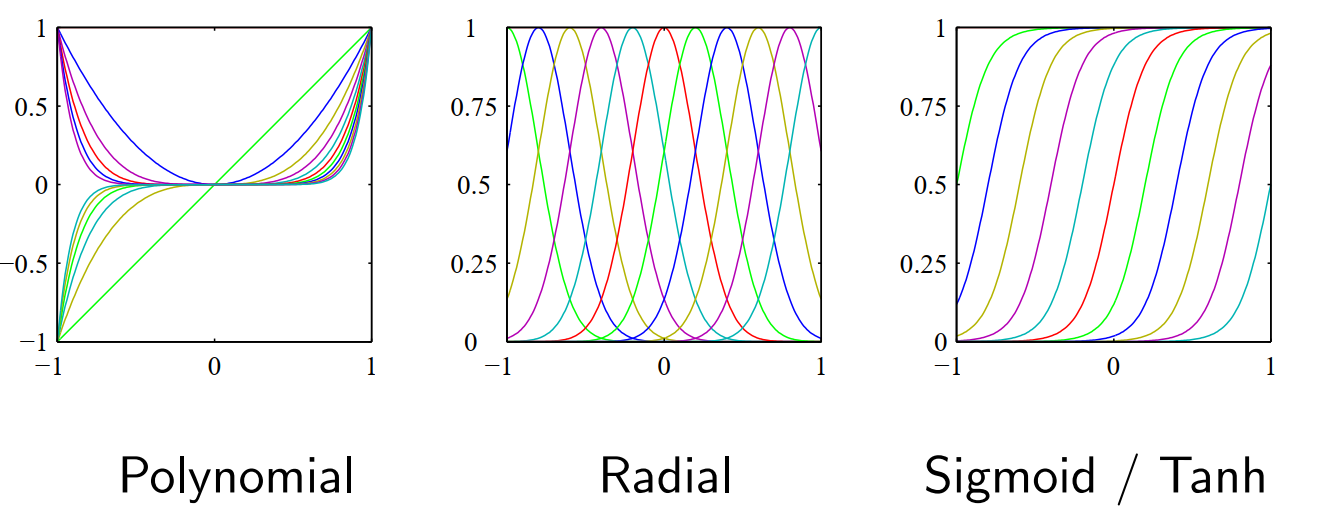
\includegraphics[width=0.9\textwidth]{basis_function_ex.png}
    \caption{ Visualizzazione grafica di alcuni esempi di basis function.}
    \label{fig:polynomial_basis}
\end{figure}

\section{Stima dei parametri: massima verosimiglianza e minimi quadrati}

Si assume che il valore target sia affetto da rumore additivo gaussiano:
\[
t = y(x; w) + \varepsilon,
\qquad \varepsilon \sim \mathcal{N}(0, \beta^{-1}),
\]
da cui segue:
\[
P(t|x,w,\beta) = \mathcal{N}(t|y(x; w), \beta^{-1}).
\]
Assumendo osservazioni indipendenti e identicamente distribuite, la massimizzazione della verosimiglianza equivale alla minimizzazione dell’errore quadratico:
\[
E_D(w) = \frac{1}{2} \sum_{n=1}^{N} \left(t_n - w^T \phi(x_n)\right)^2.
\]

Introducendo la matrice di progetto
\[
\Phi =
\begin{bmatrix}
\phi_0(x_1) & \dots & \phi_M(x_1) \\
\vdots & & \vdots \\
\phi_0(x_N) & \dots & \phi_M(x_N)
\end{bmatrix},
\]
la soluzione in forma chiusa è:
\[
w_{ML} = (\Phi^T \Phi)^{-1} \Phi^T t,
\]
che coincide con la soluzione ai minimi quadrati ottenuta tramite pseudo-inversa.

\section{Apprendimento sequenziale}

In alternativa alla soluzione analitica, i parametri possono essere appresi in modo incrementale tramite \emph{stochastic gradient descent}:
\[
\hat{w} \leftarrow \hat{w} - \eta \nabla E_S,
\]
dove $\eta$ è il learning rate e $\nabla E_S$ è una stima del gradiente calcolata su un sottoinsieme casuale dei dati. L’algoritmo converge per valori sufficientemente piccoli di $\eta$.

\subsection{Regolarizzazione}

Per contrastare l’overfitting si introduce un termine di penalizzazione sui parametri:
\[
\arg\min_w \; E_D(w) + \lambda E_W(w),
\]
con $\lambda > 0$ fattore di regolarizzazione. 

\begin{figure}[H]
    \centering
    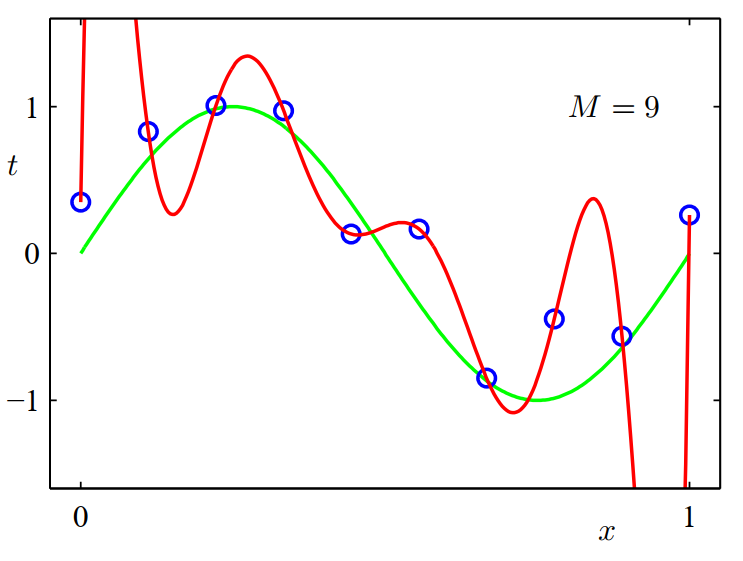
\includegraphics[width=0.70\textwidth]{regularization_effects.png}
    \caption{Effetto della regolarizzazione su un modello polinomiale di grado elevato ($M=9$). In alto è mostrata la soluzione non regolarizzata, caratterizzata da forti oscillazioni e overfitting.}
    \label{fig:regularization_effects}
\end{figure}

In assenza di penalizzazione sui parametri, un modello polinomiale di grado elevato tende ad adattarsi in modo eccessivo ai dati di training, producendo oscillazioni non giustificate e una scarsa capacità di generalizzazione.

Introducendo un termine di regolarizzazione del tipo

\[
\highlight{
E_W(w) = \frac{1}{2} w^T w,}
\]

la funzione obiettivo diventa

\[
\highlight{
E(w) = E_D(w) + \lambda E_W(w),}
\]

dove il parametro $\lambda$ controlla il compromesso tra fedeltà ai dati e complessità del modello. Per valori piccoli di $\lambda$, la penalizzazione è debole e il comportamento del modello è simile a quello non regolarizzato. All’aumentare di $\lambda$, i coefficienti vengono progressivamente ridotti, limitando le oscillazioni della funzione appresa.

\begin{figure}[H]
    \centering
    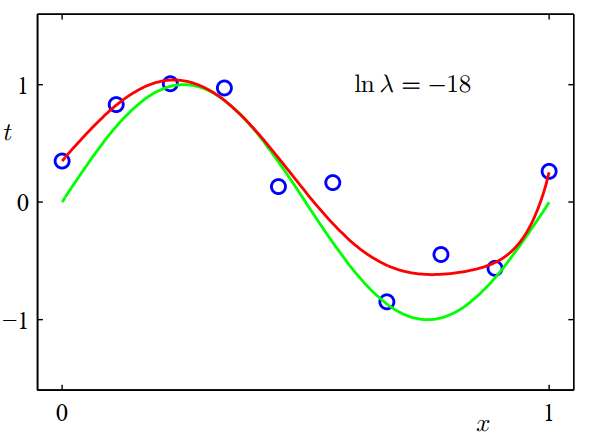
\includegraphics[width=0.70\textwidth]{regularization_effects2.png}
    \caption{Una regolarizzazione debole ($\ln \lambda = -18$), che consente una buona approssimazione della funzione target.}
    \label{fig:regularization_effects2}
\end{figure}

Un valore eccessivamente grande di $\lambda$ porta tuttavia a un modello troppo semplice, incapace di catturare la struttura dei dati, evidenziando un fenomeno di underfitting. La scelta del parametro di regolarizzazione risulta quindi cruciale per ottenere buone prestazioni di generalizzazione.

\begin{figure}[H]
    \centering
    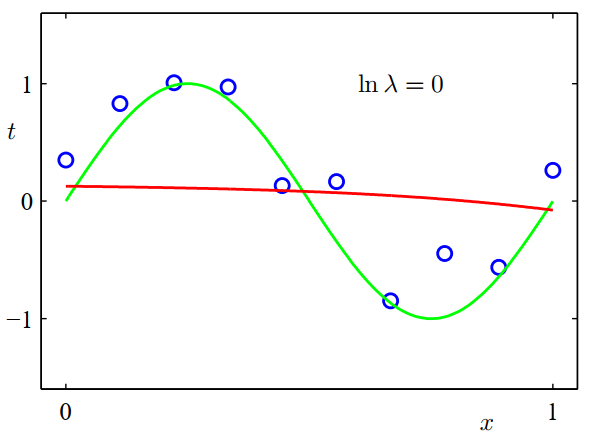
\includegraphics[width=0.70\textwidth]{regularization_effects3.png}
    \caption{Un esempio caso di regolarizzazione forte ($\ln \lambda = 0$), in cui il modello diventa eccessivamente rigido e manifesta underfitting.}
    \label{fig:regularization_effects3}
\end{figure}


\subsection{Regressione con output multipli}

Nel caso di output vettoriali $y \in \mathbb{R}^K$, il modello diventa:
\[
y(x; W) = W^T \phi(x),
\]
dove $W$ è una matrice dei parametri. Sotto le stesse ipotesi gaussiane, la stima di massima verosimiglianza è:
\[
W_{ML} = (\Phi^T \Phi)^{-1} \Phi^T T.
\]

\section*{RIEPILOGO}

\begin{tcolorbox}[
    colback=green!10,
    colframe=green!50!black,
    title=\textbf{Linear Models for Regression -- Concetti chiave},
    fonttitle=\bfseries,
    sharp corners,
    boxrule=0.8pt
]

I modelli lineari per la regressione mirano ad apprendere una funzione
\[
f : \mathbb{R}^d \rightarrow \mathbb{R}
\]
a partire da un insieme di dati etichettati, assumendo una dipendenza lineare dai parametri.

\medskip
\textbf{Modello lineare}
\[
y(x;w) = w^T x
\]
rappresenta il caso più semplice di regressione lineare.

\medskip
\textbf{Linear Basis Function Models}  
Introducendo funzioni base $\phi_j(x)$, il modello diventa:
\[
y(x;w) = \sum_{j=0}^{M} w_j \phi_j(x) = w^T \phi(x),
\]
consentendo di approssimare relazioni non lineari pur mantenendo la linearità nei parametri.

\medskip
\textbf{Stima dei parametri}  
Assumendo rumore gaussiano additivo, la massima verosimiglianza conduce alla minimizzazione dell’errore quadratico:
\[
E_D(w) = \frac{1}{2} \sum_{n=1}^{N} \left(t_n - w^T \phi(x_n)\right)^2,
\]
con soluzione in forma chiusa:
\[
w_{ML} = (\Phi^T \Phi)^{-1} \Phi^T t.
\]

\medskip
\textbf{Regolarizzazione}  
Per controllare l’overfitting si introduce una penalizzazione sui parametri:
\[
\arg\min_w \; E_D(w) + \lambda \frac{1}{2} w^T w,
\]
dove $\lambda$ regola il compromesso tra accuratezza sui dati e complessità del modello.

\medskip
In sintesi, i modelli lineari per la regressione costituiscono un quadro teorico solido e computazionalmente efficiente, ponendo le basi per tecniche più avanzate di apprendimento supervisionato.

\end{tcolorbox}

\chapter{Kernel Methods}

I metodi kernel rappresentano un’estensione fondamentale dei modelli lineari, consentendo di apprendere funzioni non lineari mantenendo una formulazione matematica elegante e computazionalmente trattabile. L’idea centrale è quella di esprimere il modello esclusivamente in termini di prodotti scalari tra campioni di input, permettendo così di sostituire tali prodotti con funzioni di similarità più generali.

\section{Dai modelli lineari alla formulazione duale}

Consideriamo un modello lineare per la regressione:
\[
y(x;w) = w^T x,
\]
e una funzione di costo regolarizzata:
\[
E(w) = \frac{1}{2}\sum_{n=1}^{N}(w^T x_n - t_n)^2 + \lambda \|w\|^2.
\]
La soluzione ottima si ottiene imponendo $\nabla E(w)=0$, da cui segue che il vettore dei pesi può essere espresso come combinazione lineare dei dati di training:
\[
w^* = \sum_{n=1}^{N} \alpha_n x_n.
\]
Sostituendo nella funzione di predizione, si ottiene:

\[
\highlight{
y(x) = \sum_{n=1}^{N} \alpha_n x_n^T x.}
\]

Questa espressione mostra che la predizione non dipende più esplicitamente dal vettore dei pesi $w$, ma solo da \textbf{quanto l’input $x$ è simile ai dati di training}. Ogni termine $x_n^T x$ misura una similarità, e i coefficienti $\alpha_n$ ne pesano l’importanza.

\section{Gram matrix e formulazione kernelizzata}

Definendo la matrice di Gram:

\[
\highlight{
K = XX^T,
\qquad K_{nm} = x_n^T x_m,}
\]
la soluzione diventa:

\[
\highlight{
\alpha = (K + \lambda I_N)^{-1} t,
\qquad
y(x) = \sum_{n=1}^{N} \alpha_n x_n^T x.}
\]
Questa formulazione è detta \emph{duale} e dipende esclusivamente dai prodotti scalari tra dati.

Il modello non “vede” più le coordinate degli input, ma solo \textbf{le relazioni reciproche} tra i punti del dataset. Questo apre la strada a una generalizzazione potente: sostituire il prodotto scalare con una misura di similarità più sofisticata.

\subsection*{Esempio}

Dato un insieme di dati di training $\{x_1,\dots,x_N\}$, la Gram matrix associata a un kernel $k$ è definita come
\[
K_{nm} = k(x_n, x_m).
\]

Consideriamo, ad esempio, tre punti bidimensionali:
\[
x_1 = \begin{bmatrix}1 \\ 0\end{bmatrix}, \quad
x_2 = \begin{bmatrix}0 \\ 1\end{bmatrix}, \quad
x_3 = \begin{bmatrix}1 \\ 1\end{bmatrix}.
\]
Utilizzando il kernel lineare $k(x,x') = x^T x'$, la Gram matrix risulta:
\[
K =
\begin{bmatrix}
1 & 0 & 1 \\
0 & 1 & 1 \\
1 & 1 & 2
\end{bmatrix}.
\]

Sostituendo il kernel lineare con un kernel gaussiano
\[
k(x,x') = \exp(-\beta \|x-x'\|^2),
\]
si ottiene una Gram matrix con la stessa struttura ma valori differenti, che riflettono una diversa nozione di similarità tra i dati.

La Gram matrix codifica quindi tutte le relazioni tra gli esempi del dataset ed è l’unico oggetto necessario per l’apprendimento nei modelli kernelizzati.


\section{Kernel functions}

Una \emph{kernel function} è una funzione:

\[
\highlight{
k : \mathcal{X} \times \mathcal{X} \rightarrow \mathbb{R},}
\]
che misura la similarità tra due input. Il kernel lineare è un caso particolare:
\[
k(x,x') = x^T x'.
\]
Sostituendo il prodotto scalare con un kernel generico, il modello diventa:

\[
\highlight{
y(x) = \sum_{n=1}^{N} \alpha_n k(x_n, x),}
\]
con

\[
\highlight{
\alpha = (K + \lambda I_N)^{-1} t,
\quad K_{nm} = k(x_n, x_m).}
\]

Il kernel può essere visto come un confronto intelligente tra esempi: invece di chiedersi “quanto sono vicini in termini di coordinate?”, il modello si chiede “quanto si assomigliano secondo un certo criterio?”.

\subsection{Kernel trick}

Il \emph{kernel trick} consiste nell’osservare che, se un algoritmo dipende dagli input \textbf{solo tramite prodotti scalari}, questi possono essere sostituiti da kernel:

\[
\highlight{
x^T x' \;\longrightarrow\; k(x,x').}
\]

In molti casi esiste una mappa implicita $\phi(x)$ tale che:

\[
\highlight{
k(x,x') = \phi(x)^T \phi(x'),}
\]

senza che sia necessario conoscere o calcolare esplicitamente $\phi(x)$.

È come lavorare in uno spazio di dimensione molto alta (o infinita) senza mai entrarci davvero. Il kernel fornisce direttamente il risultato finale, evitando il costo computazionale della trasformazione esplicita.

\subsection{Esempio: applicazione concreta del kernel trick}

Consideriamo un semplice dataset di training composto da tre esempi monodimensionali:
\[
\mathcal{D} = \{(x_1,t_1),(x_2,t_2),(x_3,t_3)\},
\quad
x_1=0,\; x_2=1,\; x_3=2,
\quad
t = \begin{bmatrix}1 \\ 0 \\ 1\end{bmatrix}.
\]

Supponiamo che un modello lineare nello spazio originale non sia sufficiente e scegliamo un kernel gaussiano (RBF):
\[
k(x,x') = \exp(-\beta (x-x')^2),
\]
con $\beta=1$.

\subsubsection*{Costruzione della Gram matrix}

La Gram matrix $K$ è definita come:
\[
K_{nm} = k(x_n,x_m).
\]
Calcolando tutte le similarità tra i punti del training, otteniamo:
\[
K =
\begin{bmatrix}
k(0,0) & k(0,1) & k(0,2) \\
k(1,0) & k(1,1) & k(1,2) \\
k(2,0) & k(2,1) & k(2,2)
\end{bmatrix}
=
\begin{bmatrix}
1 & e^{-1} & e^{-4} \\
e^{-1} & 1 & e^{-1} \\
e^{-4} & e^{-1} & 1
\end{bmatrix}.
\]

Questa matrice rappresenta completamente il dataset dal punto di vista del modello kernelizzato.

\subsubsection*{Apprendimento}

Nel caso della regressione kernelizzata con regolarizzazione, i coefficienti $\alpha$ si ottengono risolvendo:
\[
\alpha = (K + \lambda I)^{-1} t,
\]
dove $\lambda > 0$ è il parametro di regolarizzazione. Il modello non utilizza esplicitamente i dati $x_n$, ma solo la matrice $K$ e il vettore dei target $t$.

\subsubsection*{Predizione su un nuovo punto}

Dato un nuovo punto di test $x_* = 0.5$, la predizione è:
\[
y(x_*) = \sum_{n=1}^{3} \alpha_n k(x_n,x_*).
\]
In particolare:
\[
k(0,0.5)=e^{-0.25}, \quad
k(1,0.5)=e^{-0.25}, \quad
k(2,0.5)=e^{-2.25}.
\]

La predizione dipende quindi esclusivamente dalla similarità tra $x_*$ e i punti di training, senza mai calcolare esplicitamente una trasformazione non lineare dello spazio degli input.

\section{Famiglie di kernel}

Tra le famiglie di kernel più utilizzate si trovano:
\[
\begin{aligned}
&\text{Lineare: } && k(x,x') = x^T x' \\
&\text{Polinomiale: } && k(x,x') = (\beta x^T x' + \gamma)^d \\
&\text{RBF (Gaussiano): } && k(x,x') = \exp(-\beta \|x-x'\|^2) \\
&\text{Sigmoide: } && k(x,x') = \tanh(\beta x^T x' + \gamma).
\end{aligned}
\]

Ogni kernel introduce una diversa nozione di vicinanza: il kernel RBF, ad esempio, assegna un’influenza locale ai punti, mentre il kernel polinomiale cattura interazioni globali di grado crescente.

\section{Kernelized SVM}

Nel caso delle Support Vector Machine, la soluzione ottima ha la forma:

\[
\highlight{
y(x) = \mathrm{sign}\!\left(w_0 + \sum_{n=1}^{N} \alpha_n k(x_n, x)\right),}
\]
dove solo i \emph{support vectors} hanno coefficienti $\alpha_n \neq 0$.

La decisione finale dipende solo da pochi esempi critici. Il kernel consente di costruire frontiere di decisione non lineari nello spazio originale, pur mantenendo una formulazione lineare nello spazio implicito.

\subsection{Kernelized SVM per la regressione}

Nel caso regressivo, si introduce la funzione di perdita $\varepsilon$-insensitive e un tubo di tolleranza attorno alla funzione appresa. Solo i punti che violano tale tubo contribuiscono alla soluzione:

\[
\highlight{
y(x) = \sum_{n=1}^{N} (\hat{\alpha}_n - \hat{\alpha}'_n) k(x_n, x) + w_0.}
\]

Il modello ignora piccoli errori e si concentra solo sui punti che forniscono informazione rilevante, ottenendo soluzioni sparse e robuste al rumore.

\subsection*{RIEPILOGO}

\begin{tcolorbox}[
    colback=green!10,
    colframe=green!50!black,
    title=\textbf{Kernel Methods -- Concetti chiave},
    fonttitle=\bfseries,
    sharp corners,
    boxrule=0.8pt
]

I metodi kernel permettono di estendere i modelli lineari a funzioni non lineari esprimendo il modello esclusivamente in termini di prodotti scalari tra dati.

\medskip
\textbf{Idea fondamentale}  
\[
x^T x' \;\rightarrow\; k(x,x')
\]
senza calcolare esplicitamente la trasformazione dello spazio degli input.

\medskip
\textbf{Kernel trick}  
Consente di lavorare implicitamente in spazi di dimensione elevata o infinita mantenendo una complessità computazionale gestibile.

\medskip
\textbf{Kernelized models}  
\[
y(x) = \sum_{n=1}^{N} \alpha_n k(x_n, x),
\]
con soluzione dipendente solo dalla matrice di Gram.

\medskip
\textbf{Applicazioni principali}  
Le SVM kernelizzate rappresentano uno dei metodi più efficaci per classificazione e regressione non lineare, pur richiedendo una attenta selezione degli iperparametri.

\end{tcolorbox}

\chapter{Instance Based}

Gli \textbf{instance-based methods} sono modelli \emph{non-parametrici} che non costruiscono esplicitamente un modello globale durante la fase di training, ma \emph{memorizzano l’intero dataset} e rimandano il processo di apprendimento alla fase di predizione (\emph{lazy learning}).

Nei modelli parametrici il numero di parametri è fissato e indipendente dalla dimensione del dataset.
Nei modelli non parametrici, viceversa, il numero di parametri cresce con il numero di dati disponibili.

\subsubsection{K-Nearest Neighbors (K-NN)}

Si consideri un problema di classificazione:

\[
\highlight{
f : \mathcal{X} \rightarrow \mathcal{C},
\quad
\mathcal{D} = \{(x_n, t_n)\}_{n=1}^N}
\]

Dato un nuovo campione $x$, l’algoritmo K-NN opera come segue:
\begin{enumerate}
    \item si individuano i $K$ campioni più vicini a $x$ nel dataset $\mathcal{D}$;
    \item si assegna a $x$ la classe più frequente tra i suoi $K$ vicini.
\end{enumerate}

La probabilità della classe $c$ dato $x$ è stimata come:

\[
\highlight{
p(c \mid x, \mathcal{D}, K) =
\frac{1}{K}
\sum_{x_n \in \mathcal{N}_K(x, \mathcal{D})}
\mathbb{I}(t_n = c)}
\]

dove $\mathcal{N}_K(x, \mathcal{D})$ è l’insieme dei $K$ nearest neighbors di $x$ e $\mathbb{I}(\cdot)$ è la funzione indicatrice.

\paragraph{Osservazioni}
\begin{itemize}
    \item è necessario memorizzare l’intero dataset;
    \item il metodo dipende fortemente dalla funzione di distanza scelta;
    \item per $K=1$ la frontiera di decisione induce una tassellazione di Voronoi;
    \item aumentando $K$ si ottengono regioni di decisione più lisce, riducendo l’overfitting.
\end{itemize}

\section{K-Nearest Neighbors: interpretazione geometrica}

\begin{figure}[H]
    \centering
    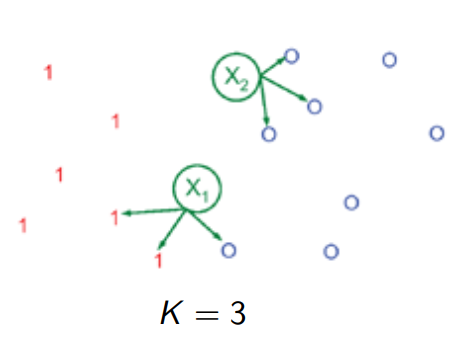
\includegraphics[width=0.55\textwidth]{knn_k3.png}
    \caption{
    Classificazione K-NN con $K=3$.  
    Per ciascun punto di query ($x_1$, $x_2$) vengono selezionati i tre campioni più vicini nel dataset; la classe assegnata è quella di maggioranza tra i vicini.  
    La decisione è locale e dipende fortemente dalla distribuzione dei punti nello spazio delle feature.
    }
    \label{fig:knn_k3}
\end{figure}

Nel caso $K>1$, la classificazione si basa su un voto di maggioranza locale, che introduce un effetto di regolarizzazione: all’aumentare di $K$, le regioni di decisione diventano più lisce e la sensibilità al rumore diminuisce, riducendo il rischio di overfitting.

\begin{figure}[H]
    \centering
    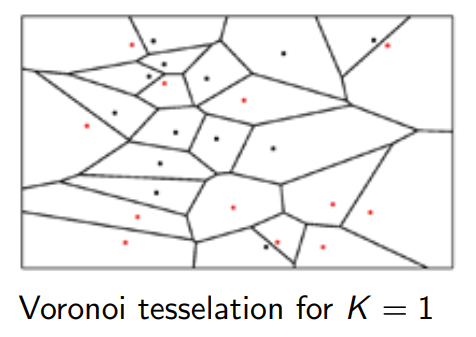
\includegraphics[width=0.75\textwidth]{voronoi_k1.png}
    \caption{
    Tassellazione di Voronoi indotta da un classificatore 1-NN ($K=1$).  
    Ogni punto del dataset genera una regione dello spazio contenente tutti i punti più vicini a esso rispetto a qualunque altro campione.  
    La frontiera di decisione risulta altamente irregolare e perfettamente adattata ai dati di training.
    }
    \label{fig:voronoi_k1}
\end{figure}

Per $K=1$, il classificatore assegna a ogni punto la classe del nearest neighbor più vicino, inducendo una tassellazione di Voronoi dello spazio delle feature.  
Questo rappresenta il caso limite di massima varianza, in cui il modello è estremamente sensibile al rumore e tende all’overfitting.

\subsection{Effetto del parametro $K$ sulle regioni di decisione}

\begin{figure}[H]
    \centering
    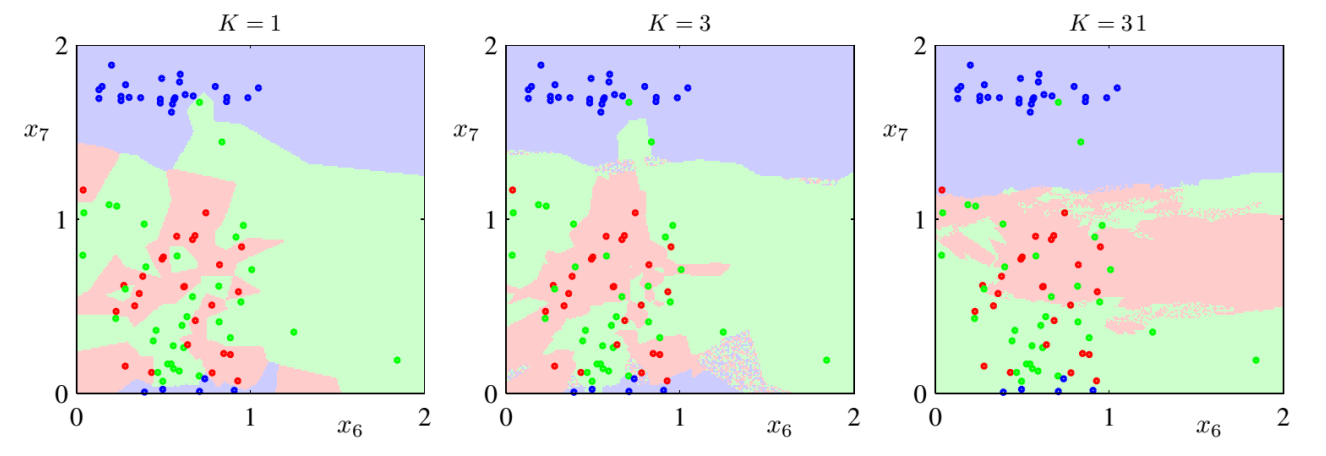
\includegraphics[width=\textwidth]{knn_increasing_k.png}
    \caption{
    Effetto dell’aumento del parametro $K$ nel classificatore K-NN.  
    Da sinistra a destra: $K=1$, $K=3$, $K=31$.  
    All’aumentare di $K$, le regioni di decisione diventano progressivamente più lisce, riducendo la complessità del modello e l’overfitting.
    }
    \label{fig:knn_increasing_k}
\end{figure}

La Figura~\ref{fig:knn_increasing_k} mostra come il valore del parametro $K$ influenzi direttamente la forma delle regioni di decisione nel classificatore K-NN.

Nel caso $K=1$, la classificazione è determinata esclusivamente dal nearest neighbor più vicino.  
Le regioni di decisione risultano altamente irregolari e frammentate, adattandosi in modo quasi perfetto ai dati di training.  
Questo comportamento corrisponde a un modello ad alta varianza, fortemente sensibile al rumore e incline all’overfitting.

Per valori intermedi di $K$ (ad esempio $K=3$), la decisione si basa su una maggioranza locale.  
Le regioni di decisione diventano più regolari, mantenendo comunque una buona capacità di catturare la struttura locale dei dati.

Per valori elevati di $K$ (ad esempio $K=31$), la classificazione tiene conto di un intorno molto ampio del punto di query.  
Le regioni di decisione risultano notevolmente più lisce e meno sensibili alle fluttuazioni locali del dataset.  
In questo regime, la varianza del modello si riduce, ma aumenta il bias, con il rischio di underfitting.

In sintesi, il parametro $K$ controlla il compromesso bias–variance del classificatore K-NN:

\[
\highlight{
K \uparrow \;\Rightarrow\; \text{decision boundaries più lisce} \;\Rightarrow\; \text{minore overfitting}}
\]

\section{Kernelized Nearest Neighbors}

Nel classificatore K-NN, la selezione dei nearest neighbors dipende dalla funzione di distanza utilizzata nello spazio delle feature.  
Nel caso della distanza euclidea al quadrato tra due punti $x$ e $x_n$:

\[
\highlight{
\|x - x_n\|^2
= (x - x_n)^T (x - x_n)
= x^T x + x_n^T x_n - 2 x^T x_n}
\]

Si osserva che la distanza può essere espressa esclusivamente in termini di prodotti scalari.  
Questo consente di applicare il \emph{kernel trick}, sostituendo il prodotto scalare con una funzione kernel:

\[
\highlight{
x^T x_n \;\longrightarrow\; k(x, x_n)}
\]

In questo modo, la distanza viene calcolata implicitamente in uno spazio delle feature ad alta (o infinita) dimensionalità:

\[
\highlight{
\|\phi(x) - \phi(x_n)\|^2
= k(x,x) + k(x_n,x_n) - 2k(x,x_n)}
\]
  
dove $\phi(\cdot)$ è una mappatura implicita associata al kernel $k(\cdot,\cdot)$.

\paragraph{Interpretazione}
Il kernelized K-NN non modifica la regola di classificazione, ma ridefinisce la nozione di vicinanza tra i punti.  
Due campioni risultano vicini se hanno un’elevata similarità nel feature space indotto dal kernel, anche se non sono vicini nello spazio originale.

\paragraph{Conseguenze}
\begin{itemize}
    \item è possibile catturare strutture non lineari nei dati;
    \item la frontiera di decisione può diventare non lineare anche nello spazio originale;
    \item la scelta del kernel influenza direttamente la geometria dello spazio delle feature e quindi i nearest neighbors.
\end{itemize}

Il kernelized K-NN rappresenta quindi un’estensione non lineare del classificatore K-NN standard, analoga concettualmente all’uso dei kernel nelle Support Vector Machines.

\section{Locally Weighted Regression}

La \emph{Locally Weighted Regression} (LWR) è un metodo di apprendimento
\emph{instance-based} e \emph{non parametrico}, in cui la funzione di regressione
non viene appresa globalmente una volta per tutte, ma viene stimata \emph{localmente}
in corrispondenza di ciascun punto di query.

A differenza della regressione lineare classica, che apprende un unico modello
valido su tutto il dominio, la LWR costruisce un modello locale utilizzando
principalmente le istanze di training vicine al punto $x_{\text{new}}$ per cui si
vuole effettuare la predizione.

\subsubsection{Idea di base}
Dato un punto di query $x_{\text{new}}$, si assegnano pesi diversi agli esempi
di training $(x_i, y_i)$ in funzione della loro distanza da $x_{\text{new}}$.
Gli esempi più vicini contribuiscono maggiormente alla stima, mentre quelli
lontani hanno un’influenza trascurabile.

La regressione viene quindi risolta come un problema di \emph{least squares pesati},
che cambia per ogni punto di query.

\subsubsection{Formulazione}
Si consideri un modello lineare locale:
\[
\hat{y}(x) = \mathbf{w}^\top \mathbf{x}
\]
I parametri $\mathbf{w}$ sono stimati minimizzando la funzione di costo:

\[
\highlight{
J(\mathbf{w}) = \sum_{i=1}^{n} w_i(x_{\text{new}})\,
\big( y_i - \mathbf{w}^\top \mathbf{x}_i \big)^2}
\]

dove $w_i(x_{\text{new}})$ è una funzione di peso che dipende dalla distanza
tra $x_i$ e il punto di query $x_{\text{new}}$.

Una scelta tipica è una funzione kernel gaussiana:

\[
\highlight{
w_i(x_{\text{new}}) =
\exp\!\left(
-\frac{\|x_i - x_{\text{new}}\|^2}{2\tau^2}
\right)}
\]

dove $\tau$ è il parametro di bandwidth che controlla l’ampiezza della regione locale.

\subsubsection{Interpretazione geometrica}
Per ogni punto di query, la LWR seleziona una regione locale del dataset e
adatta una retta (o un iperpiano) che approssima bene i dati in quella zona,
ignorando la struttura globale della funzione.

\begin{figure}[H]
\centering
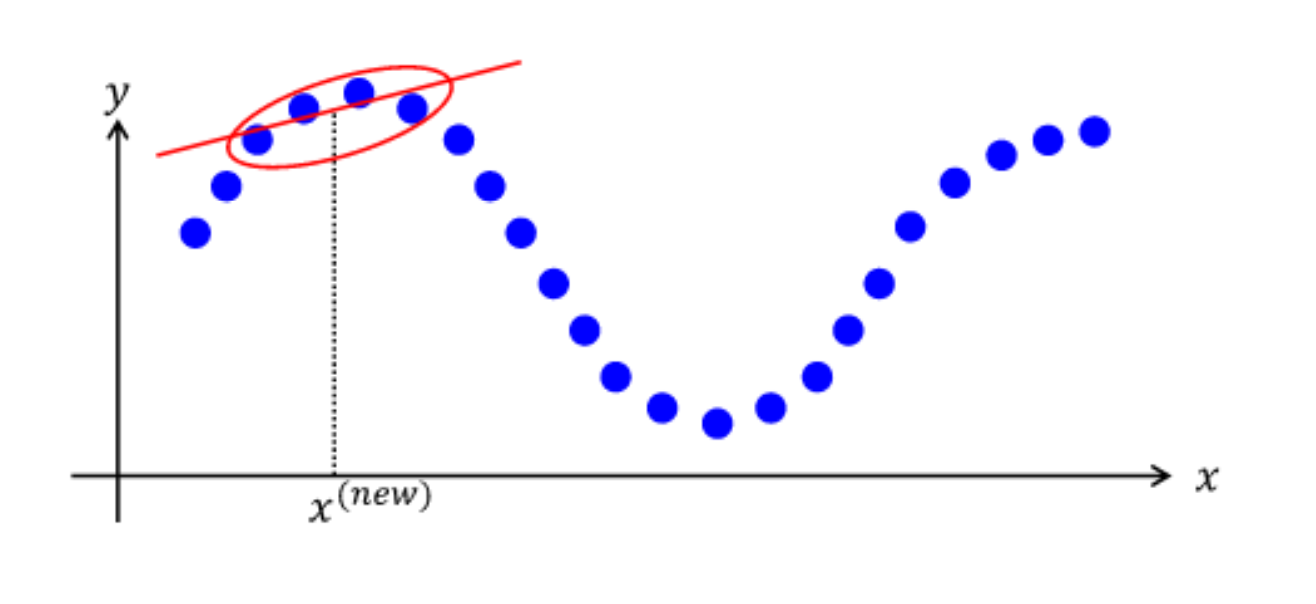
\includegraphics[width=0.7\textwidth]{locally_weighted_regression.png}
\caption{Interpretazione geometrica della Locally Weighted Regression.
Per il punto di query $x_{\text{new}}$ viene costruito un modello locale
utilizzando principalmente i punti vicini (ellisse rossa), ottenendo una
retta di regressione locale che approssima la funzione solo in quella regione.}
\end{figure}

La figura mostra come, in presenza di una funzione non lineare globale,
la LWR riesca a catturare correttamente l’andamento locale del dataset,
a differenza di un modello lineare globale che risulterebbe inadeguato.

\subsubsection{Caratteristiche principali}
\begin{itemize}
\item non esiste un modello globale esplicito;
\item l’addestramento è differito al momento della predizione;
\item elevata flessibilità e capacità di adattamento locale;
\item costo computazionale elevato in fase di test;
\item forte dipendenza dal parametro di bandwidth $\tau$.
\end{itemize}

La Locally Weighted Regression può essere vista come una generalizzazione
continua dei metodi \emph{k-nearest neighbors} per la regressione, in cui
l’influenza degli esempi non è binaria (vicino/lontano), ma decresce
progressivamente con la distanza.

\section*{RIEPILOGO}

\begin{tcolorbox}[
  colback=green!10!white,
  colframe=green!50!black,
  coltitle=white,
  title=\textbf{Instance-Based Learning – Concetti chiave},
  fonttitle=\bfseries,
  breakable
]

I metodi di \emph{Instance-Based Learning} non apprendono un modello globale
esplicito durante la fase di training, ma memorizzano il dataset e rimandano
l’apprendimento al momento della predizione.

\medskip
\textbf{Idea fondamentale}

La predizione per un punto di query $x_{\text{new}}$ viene ottenuta utilizzando
direttamente gli esempi di training più simili, secondo una misura di distanza
definita nello spazio delle feature.

\medskip
\textbf{K-Nearest Neighbors (KNN)}

Nel metodo KNN la stima dell’output è ottenuta aggregando le etichette dei $k$
vicini più prossimi a $x_{\text{new}}$.
Il parametro $k$ controlla il compromesso tra:
\begin{itemize}
\item modelli molto flessibili e sensibili al rumore ($k$ piccolo);
\item modelli più stabili ma meno adattivi ($k$ grande).
\end{itemize}

\medskip
\textbf{Kernelized Nearest Neighbors}

L’estensione kernelizzata dei KNN consente di definire la nozione di similarità
tramite funzioni kernel, permettendo di catturare strutture non lineari nei dati
senza esplicitare la mappatura nello spazio delle feature.

\medskip
\textbf{Locally Weighted Regression}

La Locally Weighted Regression costruisce, per ogni punto di query, un modello
di regressione locale risolvendo un problema di minimi quadrati pesati.
Gli esempi di training contribuiscono alla stima in modo proporzionale alla loro
vicinanza a $x_{\text{new}}$, secondo una funzione di peso (tipicamente gaussiana).
\end{tcolorbox}


\chapter{Multiple Learners}

Nei capitoli precedenti abbiamo considerato modelli di apprendimento singoli, progettati per approssimare una funzione obiettivo a partire da un insieme di dati. In questo contesto, la qualità delle prestazioni dipende fortemente dalla scelta del modello, dalla sua complessità e dalla quantità di dati disponibili. Tuttavia, anche modelli ben progettati possono risultare limitati quando affrontano problemi complessi o dati rumorosi.

L’approccio dei \emph{multiple learners}, noto anche come \emph{ensemble learning}, si basa su un’idea diversa: invece di costruire un singolo modello molto complesso, si addestrano più modelli (detti \emph{base learners}) e si combinano le loro predizioni per ottenere un risultato complessivo più accurato e robusto.

Formalmente, si considera un insieme di modelli
\[
\{y_1(x), y_2(x), \dots, y_M(x)\},
\]
addestrati sullo stesso problema, e una funzione di combinazione che produce la predizione finale a partire dalle singole uscite. I modelli possono essere addestrati in modo indipendente oppure in modo sequenziale, a seconda della strategia adottata.

L’idea alla base dell’ensemble learning è analoga al processo decisionale collettivo: una singola opinione può essere errata o influenzata dal rumore, mentre la combinazione di più punti di vista indipendenti tende a ridurre gli errori individuali. Anche se ciascun modello è relativamente semplice o imperfetto, l’insieme può produrre una decisione più affidabile.

\medskip
Un aspetto cruciale è che i modelli combinati devono essere in qualche misura \emph{diversi} tra loro. Se tutti i modelli commettono gli stessi errori, la loro combinazione non porta alcun beneficio. Le tecniche di multiple learners mirano quindi a introdurre diversità tra i modelli, sfruttandola per migliorare le prestazioni complessive.

Non è sufficiente avere molti modelli: è importante che ciascun modello “sbagli in modo diverso”. L’ensemble funziona quando gli errori dei singoli modelli si compensano a vicenda, lasciando emergere una predizione più stabile.

\medskip
Le principali strategie di ensemble learning si distinguono in base a come vengono addestrati e combinati i modelli:
\begin{itemize}
    \item combinazione di modelli addestrati in parallelo (ad esempio tramite voting o bagging);
    \item combinazione di modelli addestrati in sequenza, in cui ogni modello corregge gli errori dei precedenti (boosting).
\end{itemize}

Queste strategie, pur condividendo l’idea di base, affrontano in modo diverso il compromesso tra bias e varianza e saranno analizzate nel dettaglio nelle sezioni successive.

\section{Voting}

Una delle strategie più semplici per combinare più modelli di apprendimento è il \emph{voting}. L’idea di base consiste nell’addestrare più modelli sullo stesso dataset e combinare le loro predizioni attraverso una media (nel caso di regressione) o una maggioranza (nel caso di classificazione).

Sia dato un insieme di $M$ modelli
\[
\{y_1(x), y_2(x), \dots, y_M(x)\},
\]
addestrati a partire dallo stesso insieme di dati $\mathcal{D}$. Nel caso della regressione, la predizione combinata è definita come:

\[
\highlight{
y_{\text{voting}}(x) = \sum_{m=1}^{M} w_m \, y_m(x),}
\]

dove $w_m \geq 0$ sono pesi assegnati ai singoli modelli, tali che:

\[
\highlight{
\sum_{m=1}^{M} w_m = 1.}
\]

Nel caso della classificazione, la predizione finale è ottenuta tramite una maggioranza pesata:

\[
\highlight{
y_{\text{voting}}(x) =
\arg\max_{c}
\sum_{m=1}^{M}
w_m \, \mathbb{I}(y_m(x) = c),}
\]

dove $\mathbb{I}(\cdot)$ è la funzione indicatrice.

\begin{figure}[H]
    \centering
    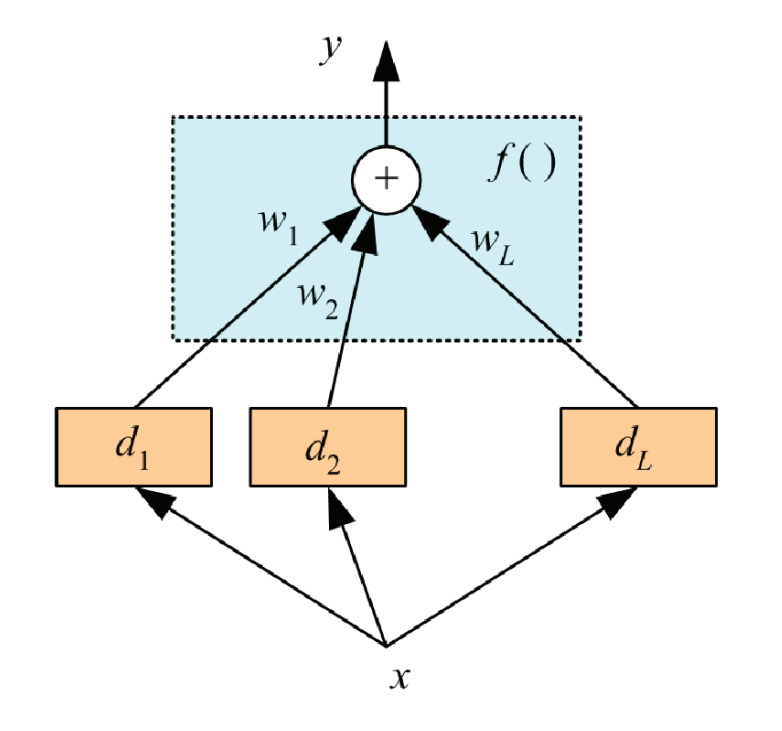
\includegraphics[width=0.65\textwidth]{voting.png}
    \caption{Schema concettuale del voting. L’input $x$ viene fornito a più modelli ($d_1, d_2, \dots, d_L$), le cui predizioni vengono combinate tramite una somma pesata per produrre l’output finale $y$.}
    \label{fig:voting}
\end{figure}

Come illustrato in Figura~\ref{fig:voting}, ogni modello produce una predizione indipendente a partire dallo stesso input. Le singole uscite vengono poi aggregate da una funzione di combinazione, che può essere vista come un modello lineare nello spazio delle predizioni.

Il voting può essere interpretato come una media delle opinioni di più esperti. Ogni modello fornisce una stima potenzialmente imperfetta, ma combinando più predizioni si riduce l’impatto degli errori individuali. Se i modelli commettono errori non correlati, questi tendono a compensarsi, producendo una predizione complessivamente più stabile.

\medskip
Nel caso in cui tutti i pesi siano uguali ($w_m = 1/M$), si parla di \emph{uniform voting}. L’introduzione di pesi differenti consente invece di assegnare maggiore importanza ai modelli ritenuti più affidabili.

\paragraph{Osservazione}
Il voting non modifica i modelli di base né il processo di addestramento: l’intervento avviene esclusivamente a livello di combinazione delle predizioni. Per questo motivo, il voting rappresenta una tecnica semplice, flessibile e facilmente parallelizzabile, ma la sua efficacia dipende fortemente dalla diversità tra i modelli combinati.

\section{Mixture of Experts}

Una generalizzazione del voting è rappresentata dal modello di \emph{mixture of experts}, in cui la combinazione delle predizioni non avviene tramite pesi fissi, ma attraverso una funzione dipendente dall’input.

Siano $d_1(x), d_2(x), \dots, d_L(x)$ un insieme di modelli di base. La predizione finale è definita come:
\[
y(x) = \sum_{l=1}^{L} g_l(x)\, d_l(x),
\]
dove $g_l(x)$ è una funzione di \emph{gating} tale che:
\[
g_l(x) \geq 0, \qquad \sum_{l=1}^{L} g_l(x) = 1.
\]

\begin{figure}[h!]
    \centering
    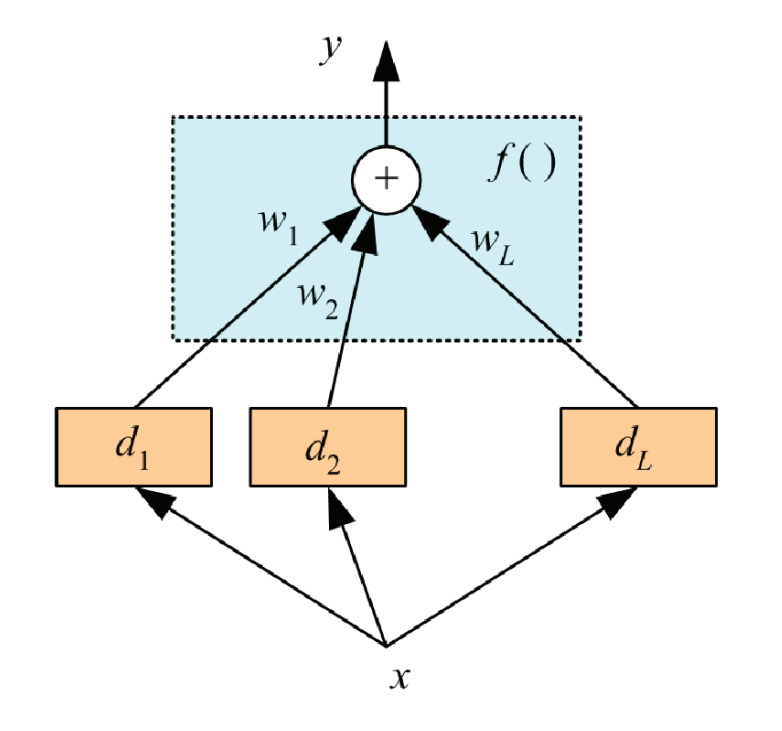
\includegraphics[width=0.7\textwidth]{mixture_of_experts.png}
    \caption{Schema del modello di mixture of experts. L’input $x$ viene fornito sia ai modelli di base ($d_1, \dots, d_L$) sia alla funzione di gating, che determina dinamicamente i pesi con cui le singole predizioni vengono combinate per produrre l’output finale $y$.}
    \label{fig:mixture_experts}
\end{figure}

A differenza del voting, in cui i pesi sono costanti, nel mixture of experts la funzione di gating apprende come selezionare o pesare i diversi modelli in base all’input.

Il mixture of experts può essere visto come un sistema adattivo che, per ogni input, decide quali modelli siano più affidabili. In questo modo, ciascun esperto può specializzarsi in una particolare regione dello spazio degli input, mentre il gating coordina il loro contributo, migliorando la capacità di modellare comportamenti complessi.

\section{Stacking}

Un’ulteriore estensione delle tecniche di ensemble è rappresentata dallo \emph{stacking}, in cui la funzione di combinazione delle predizioni viene essa stessa appresa dai dati.

Siano $d_1(x), d_2(x), \dots, d_L(x)$ un insieme di modelli di base addestrati sullo stesso problema. Nello stacking, le predizioni dei modelli di base costituiscono l’input di un meta–modello $f(\cdot)$, che produce la predizione finale:
\[
y(x) = f\big(d_1(x), d_2(x), \dots, d_L(x)\big).
\]

\begin{figure}[H]
    \centering
    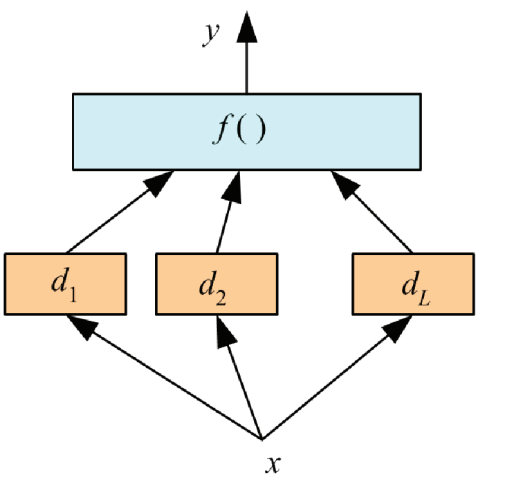
\includegraphics[width=0.65\textwidth]{stacking.png}
    \caption{Schema dello stacking. L’input $x$ viene fornito a più modelli di base ($d_1, d_2, \dots, d_L$), le cui predizioni sono utilizzate come input di un meta–modello $f(\cdot)$ che apprende come combinarle per produrre l’output finale $y$.}
    \label{fig:stacking}
\end{figure}

A differenza del voting e del mixture of experts, nello stacking non viene imposta alcuna forma specifica alla funzione di combinazione. Il meta–modello può essere qualsiasi algoritmo di apprendimento supervisionato, come una regressione lineare, una SVM o una rete neurale.

Lo stacking può essere visto come un processo di apprendimento su più livelli: i modelli di base apprendono una prima rappresentazione del problema, mentre il meta–learner apprende come sfruttare al meglio tali rappresentazioni, correggendone sistematicamente gli errori.

\section{Cascading}

Il \emph{cascading} è una tecnica di ensemble in cui i modelli di base sono organizzati in sequenza e interrogati progressivamente in base a un criterio di confidenza. A differenza di altre strategie di combinazione, nel cascading non vengono aggregate più predizioni: l’output finale è fornito da un singolo modello selezionato dinamicamente.

Siano $d_1(x), d_2(x), \dots, d_L(x)$ un insieme di modelli di base e $c_l(x)$ una misura di confidenza associata al modello $d_l$. La predizione finale è definita come:
\[
y(x) =
\begin{cases}
d_1(x) & \text{se } c_1(x) > \theta_1 \\
d_2(x) & \text{se } c_2(x) > \theta_2 \\
\vdots & \\
d_L(x) & \text{altrimenti}.
\end{cases}
\]

Il cascading può essere visto come una strategia decisionale a più stadi: modelli semplici e veloci vengono utilizzati per risolvere i casi facili, mentre modelli più complessi intervengono solo quando necessario. Questo approccio consente di ridurre il costo computazionale medio mantenendo buone prestazioni complessive.

\begin{figure}[H]
    \centering
    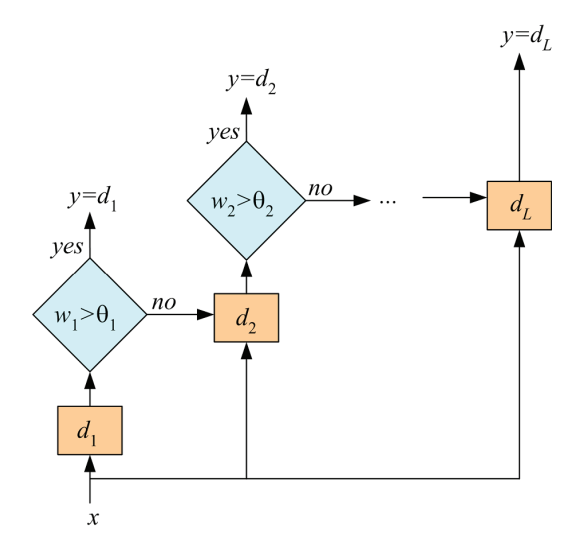
\includegraphics[width=0.75\textwidth]{cascading.png}
    \caption{Schema del cascading. L’input $x$ viene elaborato da una sequenza di modelli. Ogni modello restituisce una predizione solo se la sua confidenza supera una soglia prefissata; in caso contrario, l’input viene passato al modello successivo.}
    \label{fig:cascading}
\end{figure}

\section{Bagging}

Il \emph{bagging} (Bootstrap Aggregating) è una tecnica di ensemble learning progettata per migliorare la stabilità e la capacità di generalizzazione di un modello di apprendimento, riducendone la varianza. A differenza delle strategie viste in precedenza, il bagging introduce diversità tra i modelli non attraverso la combinazione delle predizioni o funzioni adattive, ma tramite la costruzione di differenti insiemi di addestramento.

Dato un dataset di training
\[
\mathcal{D} = \{(x_1,t_1), \dots, (x_N,t_N)\},
\]
il bagging procede secondo i seguenti passi:
\begin{enumerate}
    \item si generano $M$ dataset bootstrap $\mathcal{D}_1, \dots, \mathcal{D}_M$ mediante campionamento casuale con rimpiazzo a partire da $\mathcal{D}$;
    \item su ciascun dataset $\mathcal{D}_m$ viene addestrato un modello $y_m(x)$;
    \item le predizioni dei modelli vengono combinate tramite una media (regressione) o una maggioranza (classificazione).
\end{enumerate}

Nel caso della regressione, la predizione finale è:

\[
\highlight{
y_{\text{bagging}}(x) = \frac{1}{M} \sum_{m=1}^{M} y_m(x).}
\]

Nel caso della classificazione, si utilizza una maggioranza di voto:
\[
\highlight{
y_{\text{bagging}}(x) =
\arg\max_c
\sum_{m=1}^{M} \mathbb{I}(y_m(x)=c).}
\]

Tutti i modelli di base utilizzati nel bagging sono tipicamente dello stesso tipo e vengono addestrati in modo indipendente e parallelo.
Il bagging sfrutta il fatto che molti modelli di apprendimento, in particolare quelli complessi e flessibili (come alberi di decisione profondi), sono altamente sensibili alle variazioni del dataset di training. Piccole modifiche nei dati possono produrre modelli molto diversi.

Creando molte versioni leggermente diverse del dataset tramite bootstrap, il bagging induce una variabilità artificiale tra i modelli. La media delle loro predizioni tende a cancellare le fluttuazioni dovute al rumore, producendo una stima più stabile.

\medskip
In termini di decomposizione bias–varianza, il bagging agisce principalmente sulla \emph{varianza} del modello: non riduce significativamente il bias, ma attenua l’overfitting tipico dei modelli ad alta complessità.
Il bagging è particolarmente efficace quando i modelli di base sono instabili, ovvero quando piccole variazioni nei dati di training producono grandi variazioni nella funzione appresa. In questi casi, l’aggregazione delle predizioni consente di ottenere un miglioramento consistente delle prestazioni di generalizzazione.

\section{Boosting}

Il \emph{boosting} è una tecnica di ensemble learning in cui i modelli di base vengono addestrati in modo sequenziale, assegnando progressivamente maggiore importanza ai campioni difficili da classificare. A differenza del bagging, i modelli non sono indipendenti: ciascun learner è influenzato dalle prestazioni dei precedenti.

\begin{figure}[H]
    \centering
    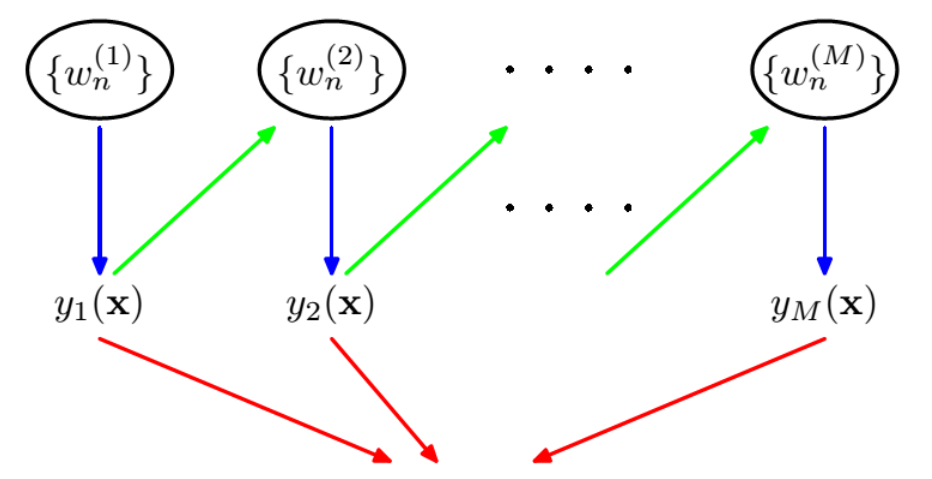
\includegraphics[width=0.80\textwidth]{boosting.png}
    \caption{Schema concettuale del boosting. A ogni iterazione $m$, il modello $y_m(x)$ viene addestrato su un dataset pesato $\{w_n^{(m)}\}$. I pesi dei campioni mal classificati vengono aumentati, costringendo i learner successivi a concentrarsi sugli errori precedenti. La predizione finale è una combinazione pesata delle predizioni dei singoli modelli.}
    \label{fig:boosting}
\end{figure}

Sia $\mathcal{D}=\{(x_n,t_n)\}_{n=1}^N$ un dataset con etichette $t_n \in \{-1,+1\}$. Il boosting costruisce una sequenza di weak learners $y_1(x), \dots, y_M(x)$, ciascuno addestrato minimizzando un errore pesato. Al termine, le predizioni vengono combinate come:

\[
\highlight{
Y_M(x) = \mathrm{sign}\!\left(\sum_{m=1}^{M} \alpha_m\, y_m(x)\right).}
\]

Il boosting può essere visto come un processo di apprendimento cooperativo: ogni modello cerca di correggere le debolezze dei precedenti, focalizzandosi sui campioni più difficili. Questo meccanismo consente di trasformare un insieme di learner deboli in un classificatore forte.

\subsection{AdaBoost}

AdaBoost (Adaptive Boosting) è uno degli algoritmi di boosting più noti ed efficaci. Il suo obiettivo è costruire un classificatore forte combinando una sequenza di classificatori deboli, ciascuno dei quali viene addestrato ponendo maggiore enfasi sui campioni che risultano difficili da classificare.

Si consideri un dataset di training
\[
\mathcal{D} = \{(x_n, t_n)\}_{n=1}^N,
\quad t_n \in \{-1, +1\}.
\]
AdaBoost mantiene una distribuzione di pesi sui campioni, indicata con

\[
\highlight{
w_n^{(m)}, \quad n=1,\dots,N,}
\]

che viene aggiornata a ogni iterazione $m$.

\subsubsection*{Algoritmo AdaBoost}

\begin{enumerate}
    \item Inizializzare i pesi dei campioni:
    \[
    w_n^{(1)} = \frac{1}{N}, \quad n = 1, \dots, N.
    \]

    \item Per $m = 1, \dots, M$:
    \begin{enumerate}
        \item addestrare un weak learner $y_m(x)$ minimizzando l’errore pesato:
        \[
        J_m = \sum_{n=1}^{N} w_n^{(m)} \, \mathbb{I}(y_m(x_n) \neq t_n);
        \]
        \item calcolare l’errore del classificatore:
        \[
        \varepsilon_m =
        \frac{\sum_{n=1}^{N} w_n^{(m)} \, \mathbb{I}(y_m(x_n) \neq t_n)}
        {\sum_{n=1}^{N} w_n^{(m)}};
        \]
        \item calcolare il peso del classificatore:
        \[
        \alpha_m = \ln\!\left(\frac{1-\varepsilon_m}{\varepsilon_m}\right);
        \]
        \item aggiornare i pesi dei campioni:
        \[
        w_n^{(m+1)} = w_n^{(m)} \exp\!\left(\alpha_m \, \mathbb{I}(y_m(x_n) \neq t_n)\right).
        \]
    \end{enumerate}
\end{enumerate}

La predizione finale è ottenuta come:

\[
\highlight{
Y_M(x) = \mathrm{sign}\!\left(\sum_{m=1}^{M} \alpha_m \, y_m(x)\right).}
\]

\begin{figure}[H]
    \centering
    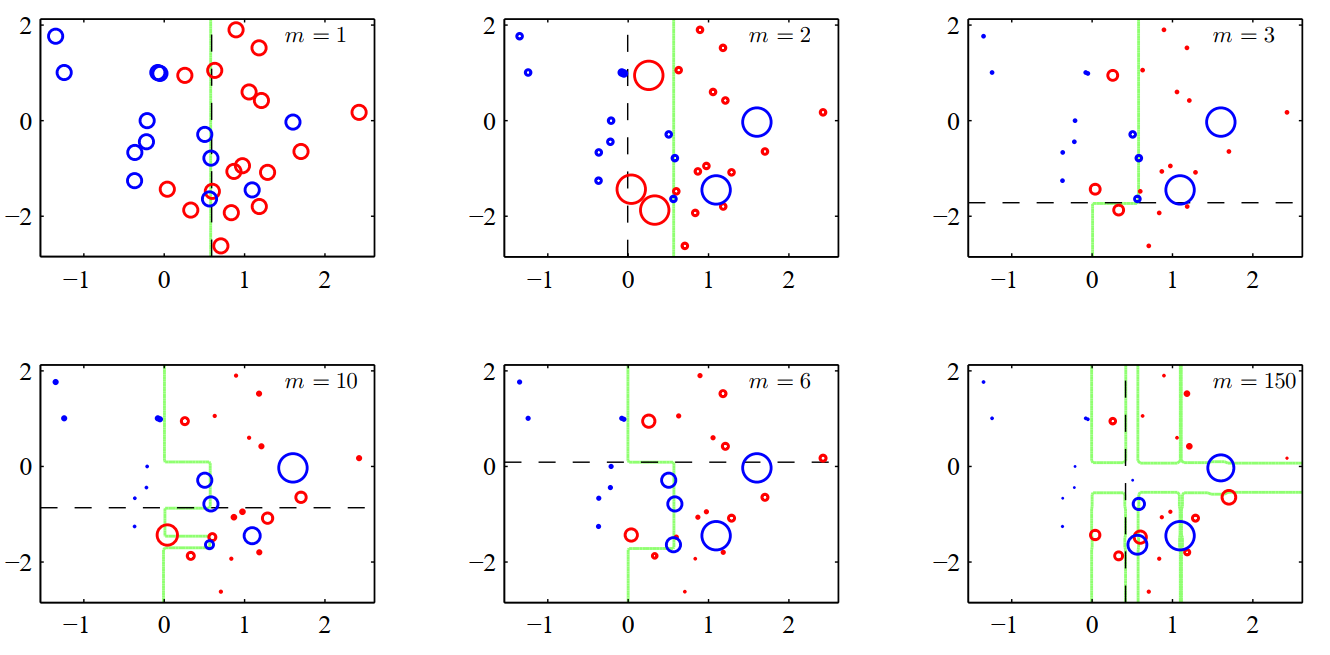
\includegraphics[width=0.95\textwidth]{adaboost_evolution.png}
    \caption{Evoluzione di AdaBoost al crescere del numero di iterazioni $m$. I cerchi più grandi indicano campioni con peso maggiore. I weak learner successivi si concentrano progressivamente sui punti difficili, producendo una frontiera di decisione sempre più articolata.}
    \label{fig:adaboost}
\end{figure}

AdaBoost può essere interpretato come un processo di apprendimento iterativo in cui, a ogni passo, il modello cerca di correggere gli errori commessi in precedenza. I campioni classificati correttamente perdono importanza, mentre quelli sbagliati vengono enfatizzati, costringendo i weak learner successivi a concentrarsi sulle regioni più difficili dello spazio degli input.

Nel corso delle iterazioni, la combinazione pesata dei classificatori produce una frontiera di decisione sempre più complessa, pur partendo da modelli molto semplici.

\subsubsection*{Remarks}

\paragraph{Vantaggi}
\begin{itemize}
    \item È semplice da implementare e computazionalmente efficiente.
    \item Non richiede una conoscenza specifica del weak learner, purché sia leggermente migliore del caso casuale.
    \item Non necessita di un’accurata scelta di iperparametri (a eccezione del numero di iterazioni $M$).
    \item Fornisce solide garanzie teoriche e ottime prestazioni empiriche in molti problemi reali.
    \item Trasforma classificatori deboli in un classificatore forte.
\end{itemize}

\paragraph{Svantaggi}
\begin{itemize}
    \item È sensibile al rumore e agli outlier, che tendono a ricevere pesi sempre più elevati.
    \item Può degradare le prestazioni in presenza di dati fortemente rumorosi o mal etichettati.
    \item La performance dipende fortemente dalla qualità dei weak learner.
    \item Può portare a modelli molto complessi se il numero di iterazioni è elevato.
\end{itemize}

\newpage
\section*{RIEPILOGO}

\begin{tcolorbox}[
    colback=green!10,
    colframe=green!50!black,
    title=\textbf{Multiple Learners -- Concetti chiave},
    fonttitle=\bfseries,
    sharp corners,
    boxrule=0.8pt,
    breakable
]

L’ensemble learning si basa sull’idea di combinare più modelli di apprendimento (\emph{base learners}) per ottenere prestazioni migliori rispetto a un singolo modello. L’efficacia di questo approccio dipende dalla diversità tra i modelli e dalla strategia di combinazione adottata.

\medskip
\textbf{Voting}  
Combina le predizioni di più modelli addestrati sullo stesso dataset mediante una media (regressione) o una maggioranza pesata (classificazione):
\[
y(x) = \sum_{m=1}^{M} w_m y_m(x).
\]
I pesi sono fissi e indipendenti dall’input.

\medskip
\textbf{Mixture of Experts}  
Generalizza il voting introducendo una funzione di \emph{gating} dipendente dall’input:
\[
y(x) = \sum_{l=1}^{L} g_l(x)\, d_l(x),
\]
consentendo ai modelli di specializzarsi in diverse regioni dello spazio degli input.

\medskip
\textbf{Stacking}  
Utilizza un meta–learner per apprendere la funzione di combinazione delle predizioni:
\[
y(x) = f(d_1(x), \dots, d_L(x)).
\]
La strategia di aggregazione non è imposta, ma appresa dai dati.

\medskip
\textbf{Cascading}  
Organizza i modelli in sequenza, utilizzando criteri di confidenza per decidere quale modello fornisce la predizione finale:
\[
y(x) = d_l(x) \quad \text{per il primo } l \text{ tale che } c_l(x) > \theta_l.
\]
È particolarmente efficace per ridurre il costo computazionale medio.

\medskip
\textbf{Bagging}  
Introduce diversità tra i modelli tramite bootstrap del dataset di training. I modelli sono addestrati in parallelo e combinati mediante media o voto:
\[
y_{\text{bagging}}(x) = \frac{1}{M} \sum_{m=1}^{M} y_m(x).
\]
Agisce principalmente riducendo la varianza.

\medskip
\textbf{Boosting e AdaBoost}  
Addestra i modelli in sequenza, ri-pesando i campioni in base agli errori precedenti:
\[
Y_M(x) = \mathrm{sign}\!\left(\sum_{m=1}^{M} \alpha_m y_m(x)\right).
\]
AdaBoost enfatizza i campioni difficili e mira a ridurre il bias del modello complessivo.

\medskip
\textbf{Bias--Variance Tradeoff}  
Le tecniche di ensemble permettono di agire sul compromesso bias–varianza:
\begin{itemize}
    \item il bagging riduce principalmente la varianza;
    \item il boosting riduce principalmente il bias;
    \item la combinazione di più learner può migliorare la robustezza al rumore.
\end{itemize}

\medskip
In sintesi, i multiple learners forniscono un potente insieme di strumenti per migliorare accuratezza, stabilità ed efficienza dei modelli di apprendimento, rappresentando una delle strategie fondamentali del machine learning moderno.

\end{tcolorbox}
 
\chapter{Artificial Neural Networks}

Le \textbf{Artificial Neural Networks (ANN)} sono modelli di apprendimento automatico parametrici progettati per approssimare funzioni complesse.  
Esse sono note anche con i seguenti nomi:
\begin{itemize}
    \item \textit{Neural Networks} (NN)
    \item \textit{Feedforward Neural Networks} (FNN)
    \item \textit{Multilayer Perceptrons} (MLP)
\end{itemize}

Le ANN sono particolarmente adatte a problemi formulabili come associazione tra vettori, ovvero alla stima di una funzione:
\[
f : \mathcal{X} \rightarrow \mathcal{Y},
\]
dove il codominio può rappresentare:
\begin{itemize}
    \item un insieme discreto di classi $\mathcal{Y} = \{C_1, \dots, C_k\}$ (classificazione),
    \item uno spazio continuo $\mathcal{Y} \subseteq \mathbb{R}^d$ (regressione).
\end{itemize}

Dato un dataset di addestramento
\[
\mathcal{D} = \{(x_n, t_n)\}_{n=1}^{N},
\]
l’obiettivo è apprendere una funzione approssimata
\[
\hat{f}(x; \theta)
\]
parametrizzata da un insieme di parametri $\theta$, tale che:
\[
\hat{f}(x_n; \theta) \approx t_n \quad \forall n.
\]

\section{Feedforward Neural Networks}

Le \textbf{Feedforward Neural Networks} sono ispirate, in modo astratto, alla struttura del cervello biologico, ma \textbf{non costituiscono un modello biologico realistico}.  
Esse sfruttano solo alcune intuizioni di base, come l’elaborazione distribuita e la composizione di unità semplici.

\begin{figure}[H]
    \centering
    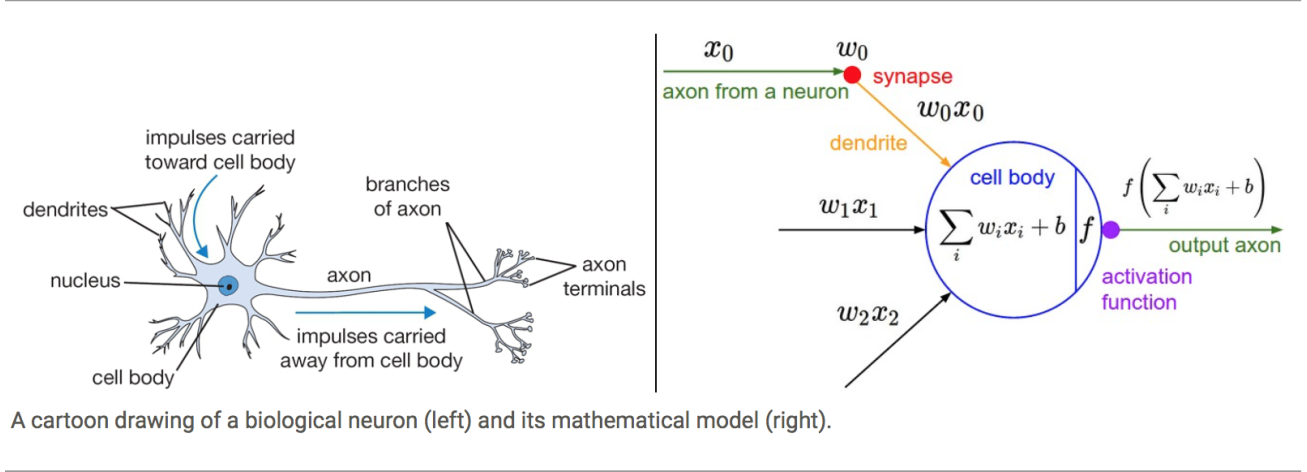
\includegraphics[width=0.95\textwidth]{neuron.png}
    \caption{}
    \label{fig:neuron}
\end{figure}

In una FNN l’informazione fluisce esclusivamente:
\[
\text{input} \;\longrightarrow\; \text{hidden layers} \;\longrightarrow\; \text{output},
\]
senza la presenza di cicli o retroazioni.

Formalmente, una rete feedforward implementa una funzione ottenuta come composizione di più trasformazioni elementari:
\[
f(x; \theta) = f^{(L)}\bigl(
f^{(L-1)}(\dots f^{(1)}(x; \theta^{(1)}) \dots ; \theta^{(L-1)})
; \theta^{(L)}
\bigr),
\]
dove:
\begin{itemize}
    \item $f^{(m)}$ rappresenta il livello $m$-esimo della rete,
    \item $\theta^{(m)}$ indica i parametri allenabili del livello $m$,
    \item $L$ è la profondità (\textit{depth}) della rete.
\end{itemize}

Le FNN hanno quindi una struttura a catena (\textit{chain structure}).  
L’ultimo livello è detto \textbf{output layer}, mentre i livelli intermedi sono detti \textbf{hidden layers}.

Il termine \textbf{Deep Learning} deriva dall’uso di reti con un numero elevato di livelli, ovvero con grande profondità.

\subsection{Perché le FNN}

Le reti feedforward superano alcune limitazioni fondamentali di altri approcci:
\begin{itemize}
    \item i \textbf{modelli lineari} non sono in grado di rappresentare interazioni non lineari tra le variabili di input;
    \item i \textbf{metodi kernel} richiedono la scelta esplicita di un kernel adeguato:
    \begin{itemize}
        \item kernel generici (RBF, polinomiali) portano a problemi convessi ma limitati in espressività;
        \item kernel progettati manualmente sono fortemente dipendenti dall’applicazione.
    \end{itemize}
\end{itemize}

Le FNN, invece, apprendono automaticamente:
\begin{itemize}
    \item combinazioni complesse di molte funzioni parametriche,
    \item modelli altamente non lineari nei parametri $\theta$,
\end{itemize}
al prezzo di un problema di ottimizzazione \textbf{non convesso}.

Questo compromesso rende le reti neurali estremamente potenti e flessibili per una vasta gamma di problemi di apprendimento automatico.

\subsection{Architettura delle Feedforward Neural Networks}

La progettazione dell’architettura di una Feedforward Neural Network (FNN) è un aspetto cruciale e comprende le seguenti scelte fondamentali:
\begin{itemize}
    \item numero di livelli nascosti (\textit{depth});
    \item numero di unità per ciascun livello (\textit{width});
    \item tipo di unità e funzioni di attivazione;
    \item funzione di costo (loss function).
\end{itemize}

Tali decisioni influenzano direttamente la capacità espressiva del modello, la sua addestrabilità e le prestazioni di generalizzazione.

\subsubsection{Modello generale di una FNN}

Una FNN è composta da più livelli completamente connessi.  
Dato un livello $i$, l’uscita del livello successivo è definita come:

\[
\highlight{
\mathbf{h}_{i+1} = f\left( \mathbf{W}_i^\top \mathbf{h}_i + \mathbf{b}_i \right),}
\]

dove:
\begin{itemize}
    \item $\mathbf{h}_i$ è il vettore delle attivazioni del livello $i$;
    \item $\mathbf{W}_i$ è la matrice dei pesi;
    \item $\mathbf{b}_i$ è il vettore dei bias;
    \item $f(\cdot)$ è una funzione di attivazione non lineare.
\end{itemize}

Il numero di parametri cresce con la dimensione dei livelli:
\[
|\mathbf{W}_i| = (\text{n. input}) \times (\text{n. output}), 
\qquad
|\mathbf{b}_i| = (\text{n. output}).
\]

\section{Profondità e Teorema di Approssimazione Universale}

Una domanda fondamentale nella progettazione delle reti neurali è:
\begin{quote}
\textit{Quanti livelli nascosti sono necessari per approssimare una funzione arbitraria?}
\end{quote}

Il \textbf{Teorema di Approssimazione Universale} fornisce una risposta teorica a questo problema.

Il teorema ci dice che una Feedforward Neural Network con:
\begin{itemize}
    \item un singolo livello nascosto,
    \item un numero sufficiente di unità nascoste,
    \item una funzione di attivazione non lineare di tipo “squashing” (ad esempio sigmoide),
    \item un livello di output lineare,
\end{itemize}
è in grado di approssimare qualsiasi funzione misurabile di Borel con un errore arbitrariamente piccolo.

Il risultato vale anche per altre funzioni di attivazione non lineari, come la \textbf{ReLU}.

\paragraph{Osservazioni importanti}
\begin{itemize}
    \item Il teorema garantisce \textbf{l’esistenza} di una rete capace di approssimare una funzione, ma non fornisce indicazioni su:
    \begin{itemize}
        \item il numero di unità necessarie;
        \item la facilità di addestramento;
        \item la qualità della generalizzazione.
    \end{itemize}
    \item Il numero di unità richieste può crescere in modo \textbf{esponenziale} con la dimensione dell’input.
\end{itemize}

\subsubsection{Larghezza vs Profondità}

Il teorema di approssimazione universale implica che, in teoria:
\begin{itemize}
    \item una rete \textbf{poco profonda ma molto larga} può approssimare qualsiasi funzione;
\end{itemize}
tuttavia, nella pratica:
\begin{itemize}
    \item reti \textbf{più profonde e più strette} risultano:
    \begin{itemize}
        \item più efficienti dal punto di vista parametrico;
        \item più facili da addestrare;
        \item migliori in termini di generalizzazione.
    \end{itemize}
\end{itemize}

Questo giustifica l’uso di architetture profonde nel \textbf{deep learning}, dove la composizione di molte trasformazioni semplici consente di rappresentare strutture complesse in modo gerarchico.

\subsubsection{Considerazioni pratiche sull’architettura}

Non esistono principi teorici generali per determinare l’architettura ottimale di una FNN.  
La progettazione è in larga parte \textbf{empirica} e dipende da:
\begin{itemize}
    \item tipo di problema;
    \item dimensione e struttura dei dati;
    \item capacità computazionali disponibili.
\end{itemize}

In sintesi, il teorema di approssimazione universale fornisce il fondamento teorico della potenza espressiva delle reti neurali, mentre le architetture profonde ne rappresentano la realizzazione pratica più efficace.

\section{Funzioni di attivazione e funzione di costo}

Una rete neurale feedforward definisce una funzione parametrica

\[
\highlight{
y = f(x;\theta),}
\]

ottenuta come composizione di trasformazioni lineari e non lineari.  
Due elementi fondamentali determinano il comportamento del modello:

\begin{itemize}
    \item le \textbf{funzioni di attivazione}, che definiscono la capacità espressiva della rete;
    \item la \textbf{loss function}, che quantifica l’errore e guida l’apprendimento.
\end{itemize}

Le funzioni di attivazione negli strati nascosti introducono non linearità nel modello.  
In assenza di tali funzioni, anche una rete profonda collasserebbe in una trasformazione lineare equivalente.

Non esistono principi teorici generali per la scelta ottimale della funzione di attivazione negli strati nascosti: la selezione è prevalentemente \textbf{empirica}.


\subsection{Funzioni di attivazione dell’output layer}

La funzione di attivazione dell’output layer dipende direttamente dal tipo di problema da risolvere.  
La scelta dell’output unit e della funzione di costo è infatti strettamente legata all’interpretazione probabilistica dell’output del modello.

Sia $\mathbf{h} = f(\mathbf{x}; \theta^{(n-1)})$ l’output dell’ultimo hidden layer.  
L’output della rete è dato da.

\[
\highlight{
\mathbf{y} = f^{(n)}(\mathbf{h}; \theta^{(n)}),}
\]
dove la funzione $f^{(n)}$ viene scelta in funzione del task.

\subsubsection{Regressione}

Nel caso di problemi di regressione, l’output layer utilizza unità lineari, ovvero la funzione di identità:

\[
\highlight{
y = \mathbf{w}^T \mathbf{h} + b.}
\]

Si assume un modello di rumore Gaussiano:
\[
p(t \mid \mathbf{x}) = \mathcal{N}(t \mid y, \beta^{-1}),
\]
per cui la massimizzazione della log-verosimiglianza equivale alla minimizzazione della \textbf{mean squared error (MSE)}.

Le unità lineari non saturano e sono quindi adatte alla predizione di valori reali non limitati, inoltre
consentono alla rete di predire valori continui non limitati e di non distorcere il valore stimato.
Questa scelta è particolarmente appropriata quando il target appartiene a $\mathbb{R}$ e quando la funzione di perdita adottata è l’errore quadratico medio (Mean Squared Error, MSE).

\subsubsection{Classificazione binaria}

Per problemi di classificazione binaria, l’output layer utilizza la funzione di attivazione \textbf{sigmoid}:

\[
\highlight{
y = \sigma(\mathbf{w}^T \mathbf{h} + b).}
\]

L’output $y$ può essere interpretato come una probabilità.  
Il modello di verosimiglianza corrisponde a una distribuzione di Bernoulli e la funzione di costo associata è la \textbf{binary cross-entropy}, ovvero la negative log-likelihood.

In questo caso, l’unità di output satura solo quando il modello fornisce una predizione corretta con alta confidenza.

\subsubsection{Classificazione multi-classe}

Nel caso di classificazione multi-classe, l’output layer è costituito da più unità e utilizza la funzione di attivazione \textbf{softmax}:

\[
\highlight{
y_i = \text{softmax}(\alpha^{(i)}) = 
\frac{\exp(\alpha^{(i)})}{\sum_j \exp(\alpha^{(j)})},
\qquad
\alpha^{(i)} = \mathbf{w}_i^T \mathbf{h} + b_i.}
\]

La softmax produce una distribuzione di probabilità sulle classi.  
La funzione di costo associata è la \textbf{categorical cross-entropy}, che corrisponde alla negative log-likelihood di una distribuzione multinomiale.

Le unità di output saturano solo in presenza di errori minimi, favorendo una maggiore stabilità dell’addestramento.


\subsection{Funzioni di attivazione nell'hidden layer}

Negli \textbf{hidden layer}, la funzione di attivazione ha lo scopo principale di introdurre non linearità nel modello, permettendo alla rete di apprendere rappresentazioni complesse e non linearmente separabili dei dati. In questo contesto, la funzione di attivazione non è vincolata all’interpretazione dell’output, ma è scelta per favorire la capacità espressiva e la stabilità dell’addestramento.

\subsubsection{Rectified Linear Unit (ReLU)}
La funzione di attivazione più utilizzata è la \textbf{Rectified Linear Unit}:

\[
\highlight{
g(\alpha) = \max(0, \alpha).}
\]

Proprietà principali:
\begin{itemize}
    \item semplicità computazionale;
    \item comportamento lineare per $\alpha > 0$;
    \item mitigazione del problema del gradiente che svanisce;
    \item non differenziabilità in $\alpha = 0$, irrilevante nella pratica.
\end{itemize}

\begin{figure}[H]
    \centering
    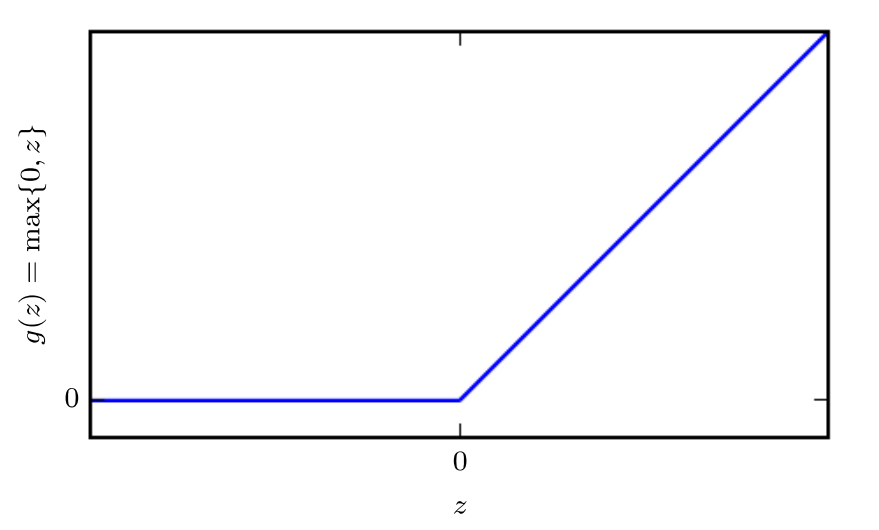
\includegraphics[width=0.95\textwidth]{ReLu.png}
    \caption{Reappresentazione matematica della ReLu}
    \label{fig:neuron}
\end{figure}


Le ReLU risultano particolarmente adatte a reti profonde.

\subsubsection{Sigmoide e tangente iperbolica}
Altre funzioni storicamente utilizzate sono:

\[
\highlight{
g(\alpha) = \sigma(\alpha),
\qquad
g(\alpha) = \tanh(\alpha),}
\]

con la relazione:

\[
\highlight{
\tanh(\alpha) = 2\sigma(2\alpha) - 1.}
\]

Entrambe sono funzioni di tipo “squashing” e soffrono di saturazione:
\begin{itemize}
    \item per grandi valori di $|\alpha|$ la derivata tende a zero;
    \item il gradiente si attenua attraversando la rete;
    \item l’apprendimento basato sul gradiente risulta lento.
\end{itemize}

La funzione $\tanh$ fornisce gradienti leggermente più grandi rispetto alla sigmoide ed è talvolta preferita in contesti specifici.

\begin{figure}[H]
    \centering
    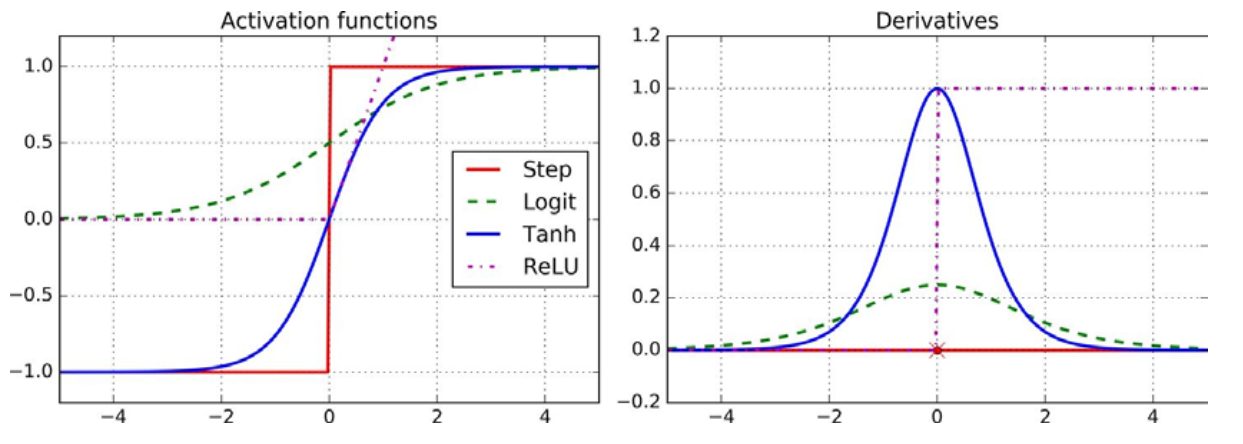
\includegraphics[width=0.95\textwidth]{activation_function.png}
    \caption{Confronto tra le principali funzioni di attivazione e le loro derivate.}
    \label{fig:neuron}
\end{figure}



\subsubsection{Output della rete e interpretazione probabilistica}

Sia $\mathbf{h}$ l’output dell’ultimo strato nascosto.  
La rete neurale definisce implicitamente una distribuzione condizionata:
\[
p(t \mid x, \theta),
\]
che dipende dalla forma dell’output e dalla funzione di attivazione utilizzata nell’ultimo strato.

La scelta dell’attivazione di output \textbf{non è indipendente} dalla funzione di costo, ma ne costituisce parte integrante.

\subsection{Loss function e principio di massima verosimiglianza}

L’addestramento della rete consiste nella minimizzazione della loss function:
\[
J(\theta) = \mathbb{E}_{x,t \sim \mathcal{D}} \bigl[ - \log p(t \mid x, \theta) \bigr],
\]
che deriva dal principio di \textbf{Massima Verosimiglianza (MLE)}.

La forma esplicita della loss dipende dall’ipotesi fatta sulla distribuzione del target.

\paragraph{Regressione}
Per problemi di regressione si utilizza un output lineare:
\[
y = \mathbf{W}^\top \mathbf{h} + \mathbf{b}.
\]

Assumendo rumore gaussiano:
\[
p(t \mid x, \theta) = \mathcal{N}(t \mid y, \beta^{-1}),
\]
la massimizzazione della verosimiglianza equivale alla minimizzazione della
\textbf{Mean Squared Error (MSE)}:
\[
J(\theta) =
\mathbb{E}_{x,t \sim \mathcal{D}}
\left[
\frac{1}{2}\lVert t - f(x;\theta) \rVert^2
\right].
\]

Le unità di output lineari non saturano, favorendo un apprendimento stabile.

\paragraph{Classificazione binaria}
Nel caso di classificazione binaria, il target $t \in \{0,1\}$ è modellato come variabile di Bernoulli:
\[
y = \sigma(\mathbf{w}^\top \mathbf{h} + b),
\quad
p(t \mid x, \theta) = y^t(1-y)^{1-t}.
\]

La loss function associata è la \textbf{Binary Cross-Entropy}:
\[
J(\theta) =
\mathbb{E}_{x,t \sim \mathcal{D}}
\bigl[
- t \log y - (1-t) \log (1-y)
\bigr].
\]

\paragraph{Classificazione multiclasse}
Per problemi di classificazione multiclasse si utilizza la funzione \textbf{softmax}:
\[
y_i = \frac{\exp(\alpha_i)}{\sum_j \exp(\alpha_j)},
\quad
\alpha_i = \mathbf{w}_i^\top \mathbf{h} + b_i.
\]

La loss function è la \textbf{Categorical Cross-Entropy}:
\[
J(\theta) =
\mathbb{E}_{x,t \sim \mathcal{D}}
\left[
- \sum_{i=1}^{K} \mathbb{I}(t=i)\log y_i
\right].
\]

\section{Calcolo del gradiente}

L’addestramento di una rete neurale consiste nella minimizzazione della loss function
\[
J(\theta),
\]
rispetto ai parametri $\theta$ del modello.  
Per questo motivo è necessario calcolare il \textbf{gradiente della loss} rispetto a tutti i parametri della rete:
\[
\nabla_{\theta} J(\theta).
\]

\subsubsection{Flusso dell’informazione}

Il funzionamento di una rete neurale può essere descritto attraverso due fasi distinte:

\begin{itemize}
    \item \textbf{forward pass}: l’informazione fluisce dall’input all’output per calcolare
    \[
    y = f(x;\theta)
    \]
    e il valore della loss $J(\theta)$;
    \item \textbf{backward pass}: l’informazione fluisce in senso inverso per calcolare i gradienti della loss rispetto ai parametri.
\end{itemize}

Il calcolo del gradiente è quindi strettamente legato alla struttura composita della funzione implementata dalla rete.

\subsubsection{Obiettivo del calcolo del gradiente}

Dato un dataset $\mathcal{D}$, l’obiettivo è determinare:
\[
\nabla_{\theta} J(\theta) =
\left(
\frac{\partial J}{\partial \theta_1},
\frac{\partial J}{\partial \theta_2},
\dots
\right),
\]
dove ciascun parametro $\theta_i$ può rappresentare un peso o un bias in uno qualsiasi dei livelli della rete.

Dal punto di vista analitico, il calcolo del gradiente è:
\begin{itemize}
    \item concettualmente semplice, poiché basato sulla regola della catena;
    \item potenzialmente costoso dal punto di vista computazionale se eseguito in modo ingenuo.
\end{itemize}

\subsubsection{Regola della catena}

La rete neurale è una composizione di funzioni.  
Nel caso scalare, se:
\[
y = g(x),
\qquad
z = f(y),
\]
la derivata di $z$ rispetto a $x$ è:
\[
\frac{dz}{dx} = \frac{dz}{dy} \frac{dy}{dx}.
\]

Nel caso vettoriale, con:
\[
g : \mathbb{R}^m \rightarrow \mathbb{R}^n,
\qquad
f : \mathbb{R}^n \rightarrow \mathbb{R},
\]
vale:
\[
\frac{\partial z}{\partial x_i}
=
\sum_{j}
\frac{\partial z}{\partial y_j}
\frac{\partial y_j}{\partial x_i},
\]
oppure, in notazione compatta:
\[
\nabla_x z =
\left(
\frac{\partial \mathbf{y}}{\partial \mathbf{x}}
\right)^{\!\top}
\nabla_{\mathbf{y}} z,
\]
dove $\frac{\partial \mathbf{y}}{\partial \mathbf{x}}$ è la matrice Jacobiana della funzione $g$.

\section{ Back-propagation}

La \textbf{back-propagation} è il meccanismo che rende possibile l’addestramento delle reti neurali profonde.  
Dal punto di vista concettuale, essa risponde a una domanda fondamentale:

\begin{quote}
\textit{in che modo ogni singolo parametro della rete contribuisce all’errore finale?}
\end{quote}

e serve a:
\begin{itemize}
    \item calcolare in modo efficiente il gradiente $\nabla_{\theta} J(\theta)$;
    \item attribuire a ciascun parametro una \textbf{responsabilità} rispetto all’errore;
    \item rendere applicabili algoritmi di ottimizzazione basati sul gradiente.
\end{itemize}

Senza back-propagation, il costo computazionale del calcolo del gradiente crescerebbe in modo proibitivo con la profondità della rete.

\subsubsection{Idea concettuale}

La back-propagation si fonda interamente sull’applicazione sistematica della regola della catena a funzioni composte.  
Una rete neurale può infatti essere vista come una funzione ottenuta dalla composizione di molte trasformazioni elementari, ciascuna delle quali dipende dai parametri di un singolo livello.

Consideriamo una funzione scalare $J$ che dipende da una variabile intermedia $y$, la quale a sua volta dipende da un’altra variabile $x$.  
In questo caso, la regola della catena afferma che la variazione di $J$ rispetto a $x$ può essere espressa come il prodotto della variazione di $J$ rispetto a $y$ e della variazione di $y$ rispetto a $x$.  
Questo principio elementare è esattamente ciò che la back-propagation applica in modo ricorsivo lungo l’intera rete.

Nel contesto di una rete neurale, la loss function dipende direttamente dall’output del modello, ma solo indirettamente dai parametri dei livelli più profondi.  
La back-propagation inizia quindi dal calcolo della derivata della loss rispetto all’output della rete.  
Questa quantità rappresenta l’errore osservato in uscita e costituisce il punto di partenza per la propagazione all’indietro.

Una volta noto come la loss varia rispetto all’output, la regola della catena permette di determinare come tale variazione dipenda dalle attivazioni dell’ultimo livello nascosto.  
Questo avviene moltiplicando il gradiente in uscita per la derivata della funzione che mappa le attivazioni nascoste nell’output.  
Il risultato è una misura di quanto ciascuna attivazione nascosta abbia contribuito all’errore finale.

Lo stesso ragionamento viene poi applicato iterativamente ai livelli precedenti.  
A ogni passaggio, il gradiente viene trasformato attraverso la derivata della funzione di attivazione del livello corrente e attraverso i pesi che collegano il livello al successivo.  
In questo modo, l’informazione sull’errore viene trasportata all’indietro lungo la rete, mantenendo una corrispondenza precisa tra ogni parametro e il suo contributo alla loss.

Dal punto di vista matematico, la back-propagation non introduce nuove regole di derivazione, ma organizza l’applicazione della regola della catena in modo efficiente e strutturato.  
Ogni derivata calcolata in un livello viene riutilizzata per il calcolo delle derivate nei livelli precedenti, evitando computazioni ridondanti.

In sintesi, la back-propagation può essere interpretata come un meccanismo che scompone la derivata globale della loss in una sequenza ordinata di derivate locali, rendendo computazionalmente praticabile il calcolo del gradiente in reti neurali profonde.


\subsection{Come si applica operativamente}

L’applicazione della back-propagation avviene sempre in due fasi distinte:

\paragraph{Forward pass}
\begin{itemize}
    \item si propaga l’input attraverso la rete;
    \item si calcolano tutte le attivazioni intermedie;
    \item si ottiene l’output finale $y$;
    \item si valuta la loss $J(\theta)$.
\end{itemize}

Durante il forward pass vengono memorizzate le quantità necessarie al calcolo del gradiente.

\paragraph{Backward pass}
\begin{itemize}
    \item si calcola il gradiente della loss rispetto all’output;
    \item si propaga il gradiente all’indietro attraverso la rete;
    \item si applica la regola della catena a ogni livello;
    \item si ottengono le derivate della loss rispetto a pesi e bias.
\end{itemize}

Ogni livello riceve:
\begin{itemize}
    \item l’informazione sull’errore dal livello successivo;
    \item la combina con la derivata della propria funzione di attivazione;
    \item produce i gradienti locali dei parametri.
\end{itemize}

\subsection{Perché è efficiente}

La back-propagation sfrutta:
\begin{itemize}
    \item la struttura aciclica del grafo computazionale;
    \item il riutilizzo delle derivate già calcolate;
    \item un approccio di programmazione dinamica.
\end{itemize}

Questo riduce drasticamente il numero di operazioni richieste rispetto a un calcolo diretto delle derivate, rendendo l’addestramento di reti profonde computazionalmente praticabile.

\section{Stochastic Gradient Descent}

Una volta calcolato il gradiente della loss function tramite back-propagation, è necessario un algoritmo che utilizzi tale informazione per aggiornare i parametri della rete.  
Il metodo di ottimizzazione più semplice e fondamentale è lo \textbf{Stochastic Gradient Descent (SGD)}.

\subsection{Idea di base}

L’obiettivo è minimizzare la funzione di costo
\[
J(\theta)
\]
aggiornando iterativamente i parametri nella direzione opposta al gradiente:

\[
\highlight{
\theta \leftarrow \theta - \eta \nabla_{\theta} J(\theta),}
\]

dove $\eta > 0$ è il \textbf{learning rate}, che controlla l’ampiezza del passo di aggiornamento.

\subsubsection{Versione stocastica}

Nel contesto delle reti neurali, il gradiente esatto sull’intero dataset è spesso troppo costoso da calcolare.  
SGD utilizza quindi una stima del gradiente calcolata su un singolo esempio o su un piccolo sottoinsieme di dati (mini-batch).

Dato un mini-batch $\{(x^{(i)}, t^{(i)})\}_{i=1}^{m}$, l’aggiornamento diventa:

\[
\highlight{
g = \frac{1}{m} \sum_{i=1}^{m} \nabla_{\theta} L\bigl(f(x^{(i)};\theta), t^{(i)}\bigr),
\qquad
\theta \leftarrow \theta - \eta g.}
\]

Questa approssimazione introduce rumore nel gradiente, ma rende l’addestramento computazionalmente efficiente e scalabile.

\subsubsection{Learning rate}

Il learning rate $\eta$ è un iperparametro critico:
\begin{itemize}
    \item valori troppo grandi possono causare instabilità o divergenza;
    \item valori troppo piccoli rallentano drasticamente la convergenza.
\end{itemize}

In pratica, $\eta$ può essere mantenuto costante oppure fatto decrescere nel tempo secondo una regola prefissata.

\subsection{SGD con momentum}

Lo \textbf{Stochastic Gradient Descent con momentum} introduce un meccanismo che consente di accelerare la convergenza e di ridurre le oscillazioni tipiche dello SGD standard.

\subsubsection{Motivazione}

Nel caso dello SGD, il gradiente stimato su mini-batch successivi può variare significativamente, soprattutto in presenza di:
\begin{itemize}
    \item superfici di costo con valli strette e allungate;
    \item direzioni con curvature molto diverse.
\end{itemize}

Questo comportamento può rallentare l’addestramento, causando oscillazioni lungo alcune direzioni e progressi lenti lungo altre.

\subsubsection{Idea del momentum}

Il momentum introduce una variabile ausiliaria, detta \textbf{velocità}, che accumula una media esponenziale dei gradienti passati.  
L’aggiornamento dei parametri non dipende quindi solo dal gradiente corrente, ma anche dalla direzione seguita nelle iterazioni precedenti.

\subsubsection{Aggiornamento dei parametri}

Siano $\eta > 0$ il learning rate e $\mu \in [0,1)$ il coefficiente di momentum.  
Le equazioni di aggiornamento sono:

\[
\highlight{
\mathbf{v}^{(k+1)} = \mu \mathbf{v}^{(k)} - \eta \mathbf{g}^{(k)},
\qquad
\theta^{(k+1)} = \theta^{(k)} + \mathbf{v}^{(k+1)},}
\]
dove $\mathbf{g}^{(k)}$ è la stima del gradiente al passo $k$.

\section{Metodi di regolarizzazione}

Le reti neurali profonde hanno un’elevata capacità espressiva, ma questa caratteristica le rende particolarmente soggette a \textbf{overfitting}, ovvero a un’eccessiva aderenza ai dati di addestramento a scapito della capacità di generalizzazione.

La \textbf{regolarizzazione} comprende un insieme di tecniche volte a ridurre l’errore di generalizzazione, introducendo vincoli o perturbazioni controllate durante l’addestramento.

\subsection{Regolarizzazione dei parametri}

Una forma comune di regolarizzazione consiste nell’aggiungere un termine di penalizzazione alla funzione di costo:

\[
\highlight{
\bar{J}(\theta) = J(\theta) + \lambda E_{\text{reg}}(\theta),}
\]

dove $E_{\text{reg}}(\theta)$ è una funzione che penalizza valori elevati dei parametri e $\lambda > 0$ controlla l’intensità della regolarizzazione.

Un esempio tipico è la penalizzazione della norma dei pesi:

\[
\highlight{
E_{\text{reg}}(\theta) = \sum_j |\theta_j|^q,}
\]

che incoraggia soluzioni più semplici e stabili.

\subsection{Dataset augmentation}

La \textbf{dataset augmentation} è una tecnica di regolarizzazione che consiste nel generare nuovi esempi di addestramento a partire da quelli esistenti, applicando trasformazioni che non alterano l’etichetta semantica dei dati.

Nel caso di immagini, esempi tipici di trasformazioni includono rotazioni, traslazioni, ridimensionamenti e variazioni di illuminazione.  
L’aggiunta di rumore è un’altra forma di augmentation utilizzata in diversi contesti.

Dal punto di vista concettuale, la dataset augmentation:
\begin{itemize}
    \item aumenta artificialmente la dimensione del dataset;
    \item riduce l’overfitting;
    \item induce invarianze desiderate nel modello.
\end{itemize}

A differenza di altre tecniche di regolarizzazione, la dataset augmentation agisce direttamente sui dati, non sui parametri o sull’algoritmo di ottimizzazione.

\subsection{Parameter sharing}

Il \textbf{parameter sharing} è una tecnica di regolarizzazione che impone vincoli sui parametri del modello, forzando diversi componenti della rete a condividere gli stessi pesi.

Questo riduce il numero totale di parametri liberi e limita la complessità effettiva del modello, migliorandone la capacità di generalizzazione.

Il parameter sharing è un elemento centrale nelle \textbf{Convolutional Neural Networks (CNN)}, dove lo stesso filtro convoluzionale viene applicato a diverse regioni dell’input.  
In questo contesto, la condivisione dei parametri:
\begin{itemize}
    \item riduce drasticamente il numero di parametri;
    \item introduce invarianza rispetto a traslazioni locali;
    \item rende l’apprendimento più efficiente e stabile.
\end{itemize}

Il parameter sharing rappresenta un esempio di come vincoli strutturali, coerenti con la natura dei dati, possano migliorare significativamente le prestazioni di una rete neurale.


\subsection{Early stopping}

L’\textbf{early stopping} è una tecnica di regolarizzazione che consiste nell’interrompere l’addestramento prima della convergenza sul training set, al fine di evitare l’overfitting.

Durante l’addestramento, la loss sul training set tende a diminuire monotonicamente, mentre la loss sul validation set inizialmente diminuisce ma può successivamente aumentare.  
Questo comportamento indica che il modello sta iniziando ad adattarsi eccessivamente ai dati di addestramento, perdendo capacità di generalizzazione.

L’early stopping arresta l’ottimizzazione nel punto in cui la loss di validazione raggiunge il minimo, utilizzando quindi un criterio basato su \textbf{cross-validation}.  

Dal punto di vista concettuale, l’early stopping agisce come una forma di regolarizzazione implicita: limita la complessità effettiva del modello senza modificare esplicitamente la funzione di costo o l’architettura della rete.

\begin{figure}[H]
    \centering
    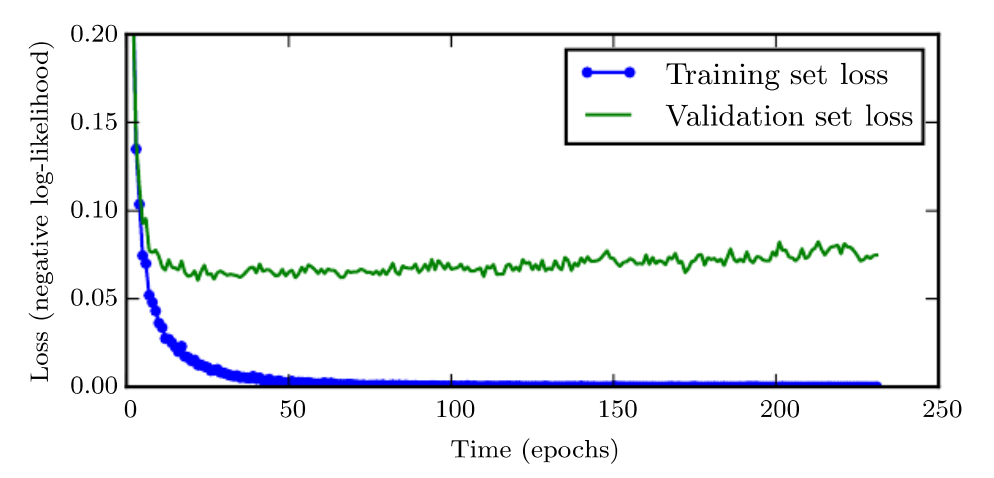
\includegraphics[width=0.85\textwidth]{early_stop.png}
    \caption{Andamento della loss sul training set e sul validation set durante l’addestramento. 
            La training loss decresce monotonicamente, mentre la validation loss, dopo una fase iniziale di miglioramento, smette di diminuire e inizia ad aumentare, indicando overfitting. 
            L’early stopping consiste nell’interrompere l’addestramento nel punto di minimo della validation loss.}
    \label{fig:early_stop}
\end{figure}

\subsection{Dropout}

Il \textbf{dropout} è una tecnica di regolarizzazione specifica per le reti neurali, che consiste nel disattivare casualmente una frazione delle unità della rete durante l’addestramento.

Ad ogni iterazione, ogni unità viene ignorata con una certa probabilità $\alpha$.  
In questo modo, la rete non può fare affidamento su percorsi specifici e viene costretta a distribuire l’informazione su più unità.

\begin{figure}[H]
    \centering
    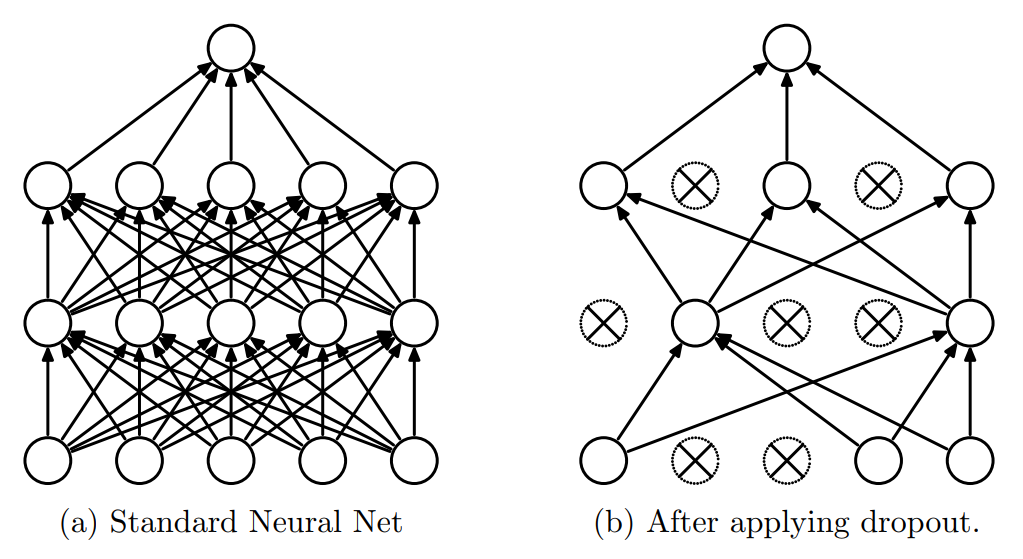
\includegraphics[width=0.80\textwidth]{dropout.png}
    \caption{Effetto del Dropout sui neuroni}
    \label{fig:dropout}
\end{figure}

Dal punto di vista concettuale, il dropout:
\begin{itemize}
    \item riduce la co-adattazione tra neuroni;
    \item agisce come una forma di ensemble implicito di reti più piccole;
    \item migliora la robustezza e la generalizzazione del modello.
\end{itemize}

\begin{figure}[H]
    \centering
    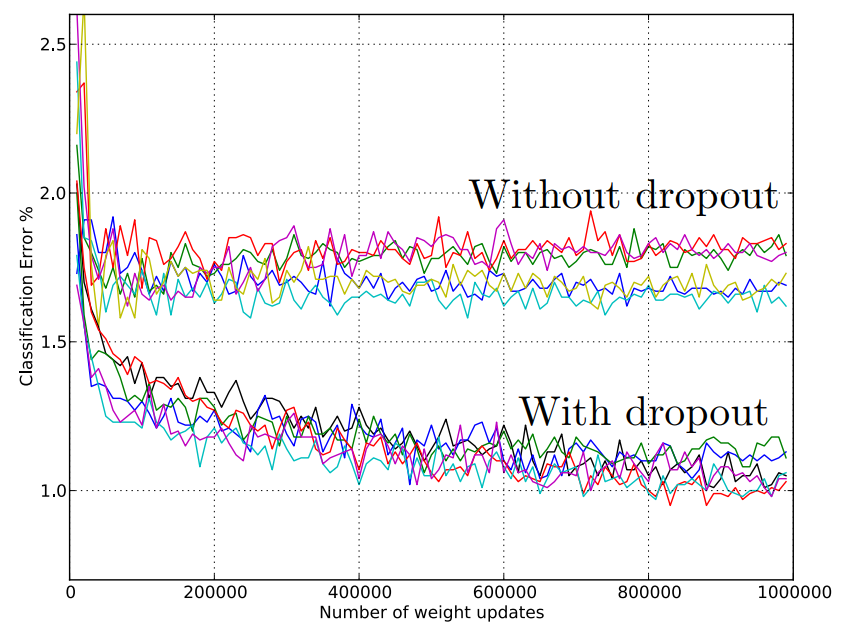
\includegraphics[width=0.85\textwidth]{dropout2.png}
    \caption{Errore di classificazione in funzione del numero di aggiornamenti dei pesi con e senza dropout. 
    Le curve con dropout mostrano un errore finale più basso e una maggiore stabilità rispetto al caso senza dropout.}
    \label{fig:dropout2}
\end{figure}

\section*{RIEPILOGO}
\begin{tcolorbox}[
    colback=green!5,
    colframe=green!50!black,
    title= Artificial Neural Networks,
    breakable
]

Le \textbf{Artificial Neural Networks (ANN)} sono modelli parametrici che approssimano funzioni complesse tramite la composizione di trasformazioni lineari e non lineari.  
In particolare, le \textbf{Feedforward Neural Networks (FNN)} implementano funzioni ottenute come catene di livelli senza cicli, caratterizzate da profondità (depth) e larghezza (width).

Il \textbf{Teorema di Approssimazione Universale} garantisce che una rete con almeno un livello nascosto e un numero sufficiente di unità possa approssimare qualsiasi funzione, ma non fornisce indicazioni sull’efficienza, sull’addestrabilità o sulla generalizzazione del modello.  
In pratica, architetture più \textbf{profonde} risultano più efficienti e generalizzano meglio rispetto a reti molto larghe e poco profonde.

Le \textbf{funzioni di attivazione} negli strati nascosti introducono non linearità e determinano la capacità espressiva della rete.  
Funzioni come ReLU sono particolarmente adatte a reti profonde poiché riducono i problemi di saturazione del gradiente.

La rete definisce implicitamente una distribuzione condizionata $p(t \mid x, \theta)$.  
La \textbf{loss function} deriva dal principio di massima verosimiglianza ed è strettamente legata all’attivazione dello strato di output:
\begin{itemize}
    \item regressione: output lineare e Mean Squared Error;
    \item classificazione binaria: sigmoide e Binary Cross-Entropy;
    \item classificazione multiclasse: softmax e Categorical Cross-Entropy.
\end{itemize}

Il \textbf{calcolo del gradiente} è reso efficiente dall’algoritmo di \textbf{back-propagation}, che applica in modo sistematico la regola della catena per propagare l’errore dall’output verso i parametri dei livelli precedenti.  
La back-propagation non aggiorna i parametri, ma fornisce le informazioni necessarie agli algoritmi di ottimizzazione.

L’ottimizzazione avviene tipicamente tramite \textbf{Stochastic Gradient Descent (SGD)} e sue varianti, come \textbf{SGD con momentum}, che accelerano la convergenza e riducono le oscillazioni.

A causa dell’elevata capacità dei modelli, le reti neurali sono soggette a overfitting.  
Per questo motivo vengono utilizzate diverse tecniche di \textbf{regolarizzazione}, tra cui:
\begin{itemize}
    \item penalizzazione dei parametri;
    \item dropout;
    \item early stopping;
    \item dataset augmentation;
    \item parameter sharing.
\end{itemize}

Queste tecniche non aumentano la capacità di approssimazione del modello, ma ne controllano la complessità effettiva, migliorando la generalizzazione.

\end{tcolorbox}

\chapter{Convolutional Neural Networks}

\section{Motivazioni}

Finora, nei modelli di apprendimento automatico e nelle Artificial Neural Networks, gli input sono stati trattati come \textbf{vettori di feature generici}.  
Questa rappresentazione è adeguata in molti contesti, ma risulta limitante quando i dati possiedono una \textbf{struttura interna} rilevante.

In numerose applicazioni reali, infatti, gli input sono segnali strutturati, come:
\begin{itemize}
    \item segnali audio, rappresentabili come vettori monodimensionali di lunghezza variabile;
    \item immagini, rappresentabili come matrici bidimensionali multi-canale;
    \item video, rappresentabili come sequenze temporali di immagini multi-canale;
    \item segnali fisici, ottenuti come campionamenti di grandezze continue.
\end{itemize}

\begin{figure}[H]
    \centering
    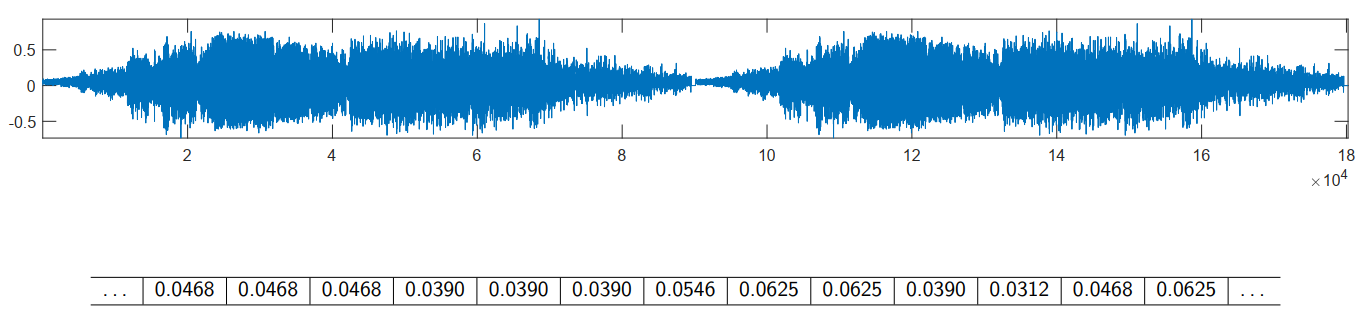
\includegraphics[width=0.95\textwidth]{audio.png}
    \caption{Un audio equivale ad avere un tensore 1D}
    \label{fig:audio}
\end{figure}

Questi dati non sono semplici vettori, ma \textbf{tensori} di diversa dimensionalità, nei quali:
\begin{itemize}
    \item esiste una nozione di località;
    \item le relazioni spaziali o temporali tra le componenti sono semanticamente rilevanti;
    \item le stesse strutture possono comparire in posizioni diverse dell’input.
\end{itemize}

\begin{figure}[H]
    \centering
    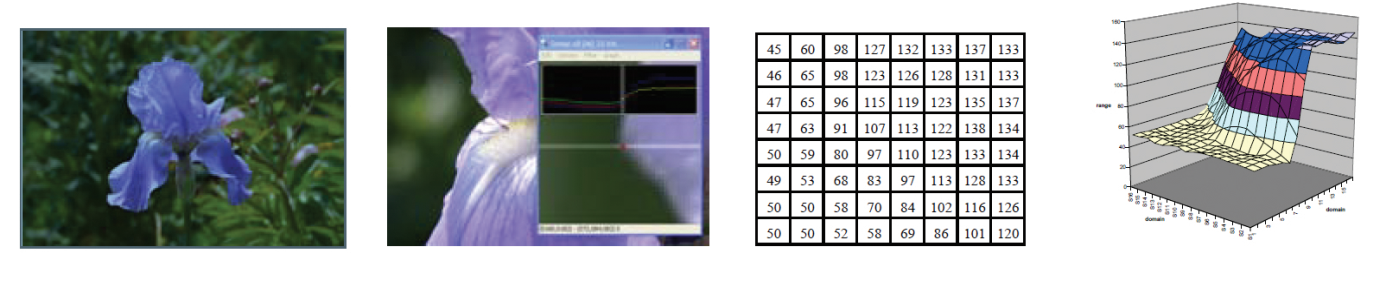
\includegraphics[width=0.95\textwidth]{immagini.png}
    \caption{Un immagine equivale ad avere una matrice 2D ed un tensore 3D}
    \label{fig:immagini}
\end{figure}

L’utilizzo di reti completamente connesse in questi casi presenta due limiti principali:
\begin{itemize}
    \item un numero di parametri molto elevato;
    \item l’incapacità di sfruttare esplicitamente la struttura locale dei dati.
\end{itemize}

Le \textbf{Convolutional Neural Networks (CNN)} nascono per superare questi limiti.

\section{Richiamo alla convoluzione}

L’operatore fondamentale alla base delle CNN è la \textbf{convoluzione}, un’operazione matematica che combina due funzioni producendo una terza funzione che misura il grado di sovrapposizione tra una funzione e una versione traslata dell’altra.

\subsubsection{Convoluzione continua}

Date due funzioni continue $x(t)$ e $w(t)$, la loro convoluzione è definita come:

\[
\highlight{
(x * w)(t) \equiv \int_{-\infty}^{+\infty} x(a)\, w(t - a)\, da.}
\]

\subsubsection{Convoluzione discreta}

Nel caso discreto, la convoluzione assume la forma:

\[
\highlight{
(x * w)(t) \equiv \sum_{a=-\infty}^{+\infty} x(a)\, w(t - a).}
\]

Questa formulazione è particolarmente rilevante per il trattamento di segnali digitali e costituisce la base delle operazioni utilizzate nelle CNN.

\subsubsection{Convoluzione bidimensionale}

Per segnali bidimensionali, come le immagini, la convoluzione discreta 2D tra un input $I$ e un kernel $K$ è definita come:

\[
\highlight{
(I * K)(i, j) \equiv 
\sum_{m \in S_1} \sum_{n \in S_2}
I(m, n)\, K(i - m, j - n),}
\]

dove $S_1$ e $S_2$ sono insiemi finiti che definiscono il supporto del kernel.

La convoluzione è un’operazione \textbf{commutativa}, a patto di effettuare il ribaltamento del kernel:
\[
(I * K)(i, j) =
\sum_{m \in S_1} \sum_{n \in S_2}
I(i - m, j - n)\, K(m, n).
\]

\begin{figure}[H]
    \centering
    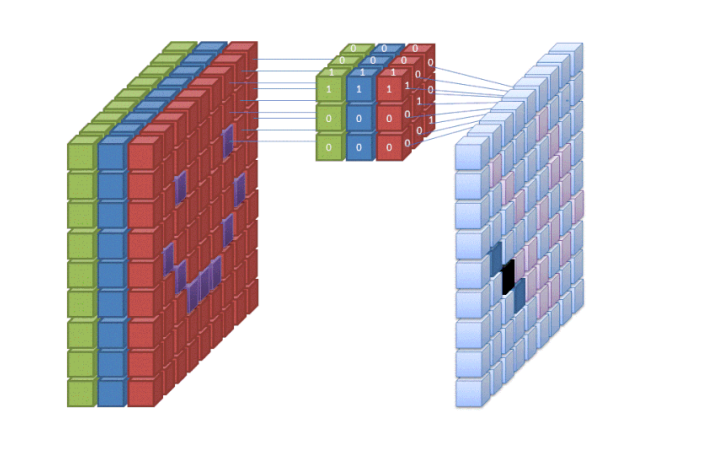
\includegraphics[width=0.80\textwidth]{CNN_2D.png}
    \caption{Schema del funzionamento di una convoluzione 2D in una Convolutional Neural Network.
            Un kernel tridimensionale, esteso su tutta la profondità dell’input, viene applicato localmente a diverse regioni dell’immagine. 
            La stessa configurazione di pesi è condivisa tra tutte le posizioni spaziali, producendo una feature map che evidenzia la presenza di uno specifico pattern indipendentemente dalla sua posizione nell’input. }
    \label{fig:CNN_2D}
\end{figure}

\subsubsection{ Convoluzione tridimensionale}

La convoluzione può essere estesa a segnali di dimensionalità superiore.  
Nel caso tridimensionale, la convoluzione discreta tra un input $I$ e un kernel $K$ è definita come:

\[
\highlight{
(I * K)(i, j, k) \equiv
\sum_{m \in S_1} \sum_{n \in S_2} \sum_{u \in S_3}
I(i + m, j + n, k + u)\, K(m, n, u).}
\]

La convoluzione 3D è utilizzata quando:
\begin{itemize}
    \item l’input possiede una struttura tridimensionale intrinseca;
    \item è necessario catturare correlazioni lungo tre dimensioni, ad esempio spazio e tempo.
\end{itemize}

\begin{figure}[H]
    \centering
    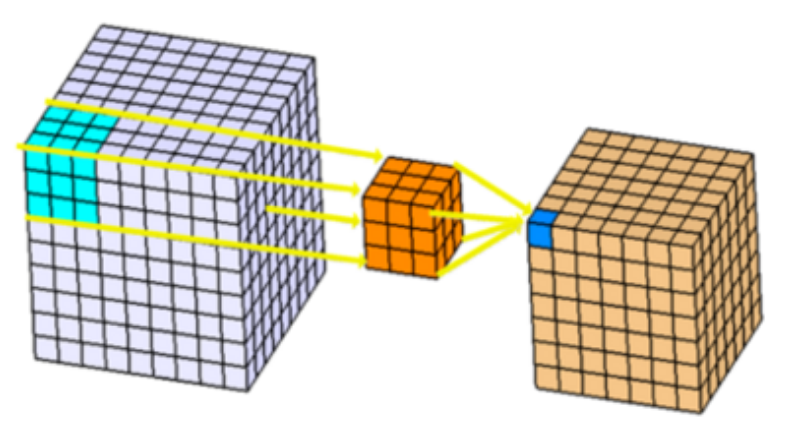
\includegraphics[width=0.80\textwidth]{CNN_3D.png}
    \caption{Un kernel tridimensionale opera su una regione locale dell’input estendendosi su tutta la profondità, combinando le informazioni       provenienti dai diversi canali. 
    Il risultato di questa operazione è un singolo valore della feature map di output, ottenuto come somma delle risposte del kernel sui vari canali. }
    \label{fig:CNN_3D}
\end{figure}

Esempi tipici includono:
\begin{itemize}
    \item video, rappresentati come sequenze temporali di immagini;
    \item dati volumetrici, come immagini medicali (CT, MRI);
    \item segnali multi-canale con dipendenza spaziale e temporale.
\end{itemize}

Nel contesto delle CNN per immagini a colori, è comune applicare una convoluzione \textbf{2D} su input \textbf{3D} (altezza, larghezza, canali), utilizzando kernel tridimensionali che si estendono su tutta la profondità dell’input.

\subsection{Cross-correlazione}

Nella pratica, molte librerie di machine learning implementano una variante detta \textbf{cross-correlazione}, definita come:

\[
\highlight{
(I * K)(i, j) =
\sum_{m \in S_1} \sum_{n \in S_2}
I(i + m, j + n)\, K(m, n).}
\]

Dal punto di vista computazionale, il fatto che non sia necessario il ribaltamento del Kernel rende l’operazione:
\begin{itemize}
    \item più semplice da implementare;
    \item più efficiente in termini di accesso alla memoria;
    \item meglio ottimizzabile su architetture parallele (GPU/TPU).
\end{itemize}

Dal punto di vista dell’apprendimento, non vi è alcuna perdita di generalità:  
poiché i valori del kernel sono parametri allenabili, la rete può apprendere automaticamente anche versioni ribaltate dei filtri, se necessario.

Per questo motivo, nel contesto delle CNN, il termine \textit{convoluzione} viene comunemente utilizzato per indicare l’operazione di cross-correlazione.

\subsection{Il kernel}

Il \textbf{kernel} è l’elemento fondamentale alla base delle Convolutional Neural Networks.  
Esso può essere visto come una piccola matrice di pesi che viene applicata localmente all’input per rilevare specifici pattern.

Nel caso di immagini bidimensionali, un kernel ha tipicamente dimensioni ridotte, ad esempio $3 \times 3$ o $5 \times 5$.  
Quando l’input presenta più canali (ad esempio immagini RGB), il kernel si estende anche lungo la dimensione dei canali, diventando un tensore tridimensionale.

I valori del kernel non sono fissati a priori, ma costituiscono \textbf{parametri allenabili} della rete.  
Durante l’addestramento, il kernel viene ottimizzato affinché risponda in modo elevato alla presenza di uno specifico pattern locale nell’input, come un bordo, un angolo o una texture.

\begin{figure}[H]
    \centering
    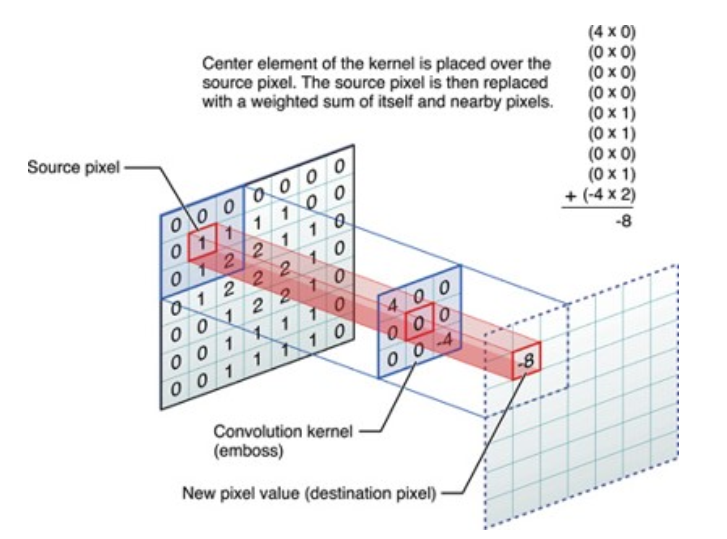
\includegraphics[width=0.85\textwidth]{kernel.png}
    \caption{}
    \label{fig:kernel}
\end{figure}

\subsection{La feature map}

Una \textbf{feature map} è il risultato dell’applicazione di un kernel sull’input tramite l’operazione di convoluzione.  
Essa può essere vista come una nuova immagine (o matrice) in cui ogni valore rappresenta la risposta del kernel in una specifica posizione dell’input.

Operativamente, mentre il kernel scorre sull’input, in ciascuna posizione viene prodotto un singolo valore di output.  
L’insieme di tutti questi valori, organizzati secondo la struttura spaziale dell’input, costituisce la feature map.

Ogni feature map è quindi associata a un singolo kernel e indica \emph{dove} il pattern cercato dal kernel è presente nell’input e con quale intensità.  
Utilizzando più kernel nello stesso convolutional layer, si ottengono più feature map, ciascuna sensibile a un pattern diverso.


\section{Convolutional Neural Networks}

Le \textbf{Convolutional Neural Networks (CNN)} sono una classe di reti neurali profonde progettate per elaborare dati strutturati, come segnali temporali, immagini e video.  
Esse estendono le Feedforward Neural Networks introducendo livelli convoluzionali, che sfruttano operatori locali e parametri condivisi per modellare in modo efficiente le dipendenze spaziali e temporali presenti nei dati.

Formalmente, una CNN è una rete feedforward composta da una sequenza di livelli specializzati, in cui almeno uno è un \textbf{convolutional layer}.  
Ogni livello convoluzionale applica un insieme di kernel all’input, producendo una collezione di \textbf{feature map} che rappresentano la presenza di pattern locali nell’input.

A differenza delle reti completamente connesse, nelle CNN:
\begin{itemize}
    \item le connessioni tra neuroni sono \textbf{locali} (sparse connectivity);
    \item gli stessi parametri sono riutilizzati su diverse regioni dell’input (parameter sharing);
    \item la struttura spaziale dell’input viene preservata attraverso i livelli.
\end{itemize}

Queste caratteristiche permettono di ridurre drasticamente il numero di parametri allenabili, migliorando sia l’efficienza computazionale sia la capacità di generalizzazione del modello.

Nel contesto delle immagini, l’input di una CNN è tipicamente rappresentato come un tensore tridimensionale, in cui due dimensioni descrivono la struttura spaziale e la terza rappresenta i canali (ad esempio RGB).  
Le convoluzioni vengono applicate localmente sulle dimensioni spaziali e globalmente sulla profondità, consentendo alla rete di apprendere filtri sensibili a pattern visivi elementari, come bordi, angoli e texture.

Una CNN è generalmente organizzata come una successione di \textbf{convolutional layers}, ciascuno seguito da una funzione di attivazione non lineare e, opzionalmente, da un livello di pooling.  
I livelli convoluzionali iniziali apprendono feature locali semplici, mentre i livelli più profondi combinano tali feature per rappresentare strutture sempre più astratte.

In sintesi, le Convolutional Neural Networks rappresentano un’evoluzione delle reti neurali classiche, in cui vincoli strutturali coerenti con la natura dei dati permettono di ottenere modelli più efficienti, robusti e scalabili per l’elaborazione di segnali strutturati.


\section{Convolutional layer}

Una \textbf{Convolutional Neural Network} può essere vista come una Feedforward Neural Network in cui uno o più livelli sono \textbf{convolutional layers}.  
Un convolutional layer non è una singola operazione, ma una trasformazione composta, articolata in più stadi applicati in sequenza allo stesso input.

In particolare, un convolutional layer è costituito da tre stadi principali:
\begin{enumerate}
    \item uno stadio di convoluzione (convolution stage);
    \item uno stadio di attivazione non lineare;
    \item uno stadio di pooling (opzionale).
\end{enumerate}

\begin{figure}[H]
    \centering
    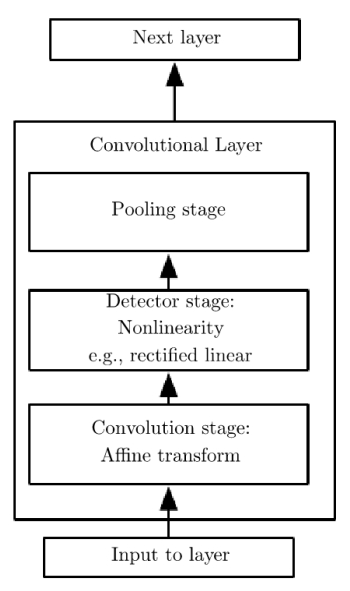
\includegraphics[width=0.50\textwidth]{convolutional_stage.png}
    \caption{}
    \label{fig:convolution_stage}
\end{figure}


\subsection{Convolution stage}

Il \textbf{convolution stage} è il primo stadio di un convolutional layer e rappresenta il momento in cui viene applicata l’operazione di convoluzione (o, in pratica, di cross-correlazione) tra l’input e un insieme di kernel.

In questo stadio, ogni kernel viene fatto scorrere sull’input e, in ciascuna posizione, produce un valore di attivazione tramite un prodotto scalare tra i pesi del kernel e una regione locale dell’input.  
Il risultato è una \textbf{feature map}, che indica la risposta del kernel nelle diverse posizioni spaziali.

Una caratteristica fondamentale del convolution stage è la \textbf{sparse connectivity}.  
A differenza delle reti completamente connesse, ogni unità di output dipende solo da un sottoinsieme limitato delle unità di input, definito dal \textbf{receptive field} del kernel.  
Questo significa che ciascun neurone è connesso soltanto a una regione locale dell’input e non all’intero volume di ingresso.

La sparse connectivity è una conseguenza diretta della struttura dell’operazione di convoluzione e non dipende né dalla funzione di attivazione né dallo stadio di pooling.  
Essa consente di ridurre significativamente il numero di connessioni e di parametri, rendendo il modello più efficiente e meglio adattato a dati con struttura spaziale o temporale.

\begin{figure}[H]
    \centering
    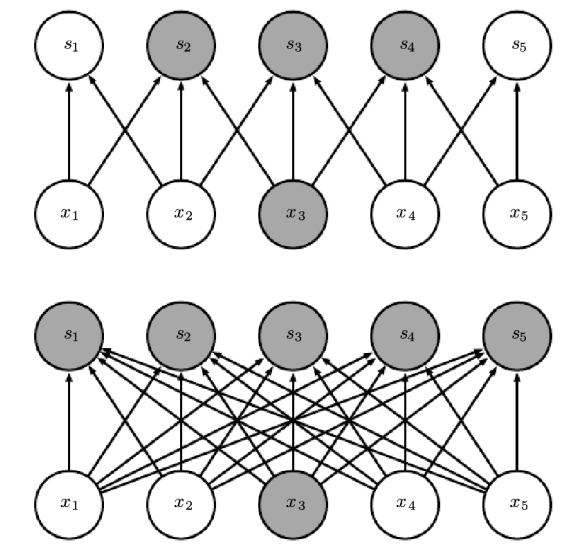
\includegraphics[width=0.70\textwidth]{sparse_connectivity.png}
    \caption{Confronto tra la connettività di un livello convoluzionale con quella di un livello completamente connesso. 
    Nella parte superiore è mostrata la \textbf{sparse connectivity}: ogni unità di output è connessa solo a un sottoinsieme locale delle unità di input, definito dal receptive field. 
    Nella parte inferiore è invece rappresentata una connessione completamente densa, in cui ogni unità di output dipende da tutte le unità di input. 
    Questo confronto evidenzia come la convoluzione riduca il numero di connessioni e parametri, sfruttando la struttura locale dei dati.}
    \label{fig:sparse_connectivity}
\end{figure}

NB: Il receptive field è la porzione dell’input che può influenzare il valore di un neurone nella feature map.

\subsubsection{Parameter sharing}

Il \textbf{parameter sharing} è una proprietà fondamentale del convolution stage e consiste nell’utilizzo degli stessi parametri del kernel in tutte le posizioni dell’input.

Quando un kernel viene fatto scorrere sull’input, i suoi pesi non cambiano da una posizione all’altra.  
Lo stesso insieme di parametri viene applicato ripetutamente a regioni locali diverse, producendo una feature map.  
Di conseguenza, tutti i neuroni appartenenti alla stessa feature map condividono gli stessi pesi.

Dal punto di vista concettuale, il parameter sharing implica che la rete non apprende un pattern specifico per ogni posizione dell’input, ma apprende \emph{che tipo di pattern} cercare, indipendentemente da dove esso compaia.  
Questo rende le CNN naturalmente adatte a dati in cui le stesse strutture possono apparire in posizioni diverse, come nel caso delle immagini.

\begin{figure}[H]
    \centering
    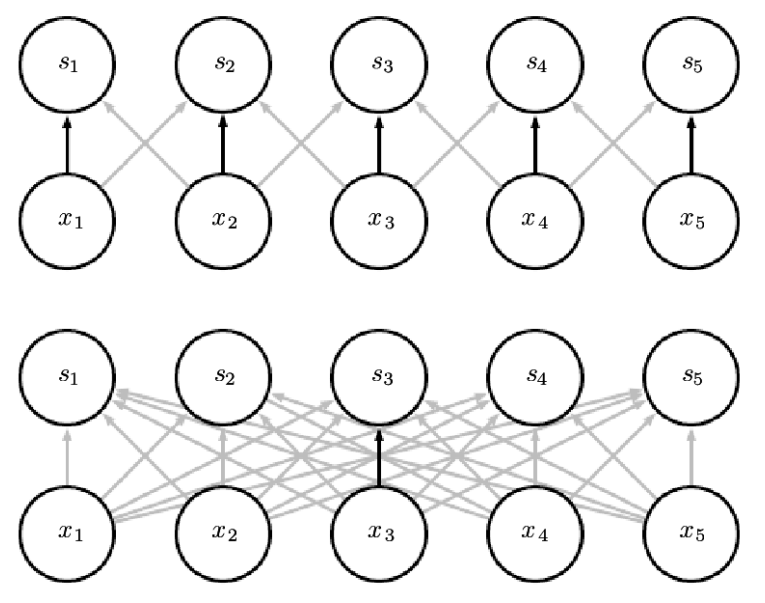
\includegraphics[width=0.70\textwidth]{parameter_sharing.png}
    \caption{}
    \label{fig:sparse_connectivity}
\end{figure}

Il parameter sharing comporta una drastica riduzione del numero di parametri rispetto alle reti completamente connesse e contribuisce in modo significativo al miglioramento della capacità di generalizzazione.  
Insieme alla sparse connectivity, esso rappresenta uno dei principali motivi per cui le Convolutional Neural Networks risultano più efficienti ed efficaci nell’elaborazione di dati strutturati.


\subsubsection{Padding}

Il \textbf{padding} è una tecnica utilizzata nel convolution stage che consiste nell’aggiungere valori artificiali ai bordi dell’input prima di applicare la convoluzione.  
Nella pratica, i valori aggiunti sono tipicamente pari a zero (\textit{zero-padding}).

L’introduzione del padding ha un effetto diretto sulla dimensione della feature map di output.  
Senza padding, il kernel può essere applicato solo alle posizioni in cui esso è completamente contenuto nell’input, causando una riduzione progressiva delle dimensioni spaziali man mano che si procede nei layer.

Il padding consente invece di:
\begin{itemize}
    \item controllare la dimensione dell’output;
    \item preservare l’informazione ai bordi dell’input;
    \item mantenere costante la risoluzione spaziale attraverso più layer convoluzionali.
\end{itemize}

In particolare, si distinguono due casi comuni:
\begin{itemize}
    \item \textbf{valid convolution}: nessun padding, con riduzione della dimensione dell’output;
    \item \textbf{same convolution}: padding scelto in modo da ottenere un output con la stessa dimensione spaziale dell’input.
\end{itemize}

Dal punto di vista concettuale, il padding permette ai neuroni convoluzionali di trattare in modo simmetrico anche le regioni vicine ai bordi dell’input, evitando che tali regioni contribuiscano meno all’apprendimento rispetto alle zone centrali.

Il padding influisce inoltre sul receptive field effettivo dei neuroni, poiché determina quante volte un pixel dell’input può essere incluso nelle operazioni di convoluzione.

\paragraph{NB}: \textbf{Il padding avviene prima della convoluzione vera e propria.}


\subsection{Detector stage}

Il \textbf{detector stage} è il secondo stadio di un convolutional layer e consiste nell’applicazione di una funzione di attivazione non lineare alle feature map prodotte dal convolution stage.

Dal punto di vista matematico, a ogni valore della feature map viene applicata una funzione

\[
\highlight{
g(\cdot),}
\]

ottenendo una nuova mappa di attivazioni.  
Una scelta comune per il detector stage è la funzione \textbf{ReLU}:

\[
\highlight{
g(x) = \max(0, x).}
\]

Il ruolo principale del detector stage è introdurre \textbf{non linearità} nel modello.  
In assenza di questo stadio, una sequenza di convoluzioni si ridurrebbe a un’unica trasformazione lineare equivalente, limitando drasticamente la capacità espressiva della rete.

Dal punto di vista concettuale, il detector stage può essere interpretato come un meccanismo di rilevazione:  
un kernel produce una risposta elevata solo quando il pattern che ha appreso è presente nella regione dell’input, e la funzione di attivazione enfatizza tali risposte, attenuando o annullando le attivazioni non rilevanti.

Il detector stage non modifica la struttura spaziale delle feature map, ma ne trasforma i valori, rendendo la rappresentazione più selettiva e adatta alla composizione di più layer convoluzionali.

\subsection{Pooling stage}

Il \textbf{pooling stage} è lo stadio finale di un convolutional layer e ha lo scopo di ridurre la dimensionalità spaziale delle feature map, mantenendo al contempo l’informazione più rilevante.

Il pooling opera localmente su ciascuna feature map, aggregando i valori all’interno di regioni spaziali limitate.  
A differenza del convolution stage, il pooling non introduce nuovi parametri allenabili, ma applica una trasformazione deterministica.

Le due operazioni di pooling più comuni sono:
\begin{itemize}
    \item \textbf{max pooling}, che seleziona il valore massimo all’interno della regione considerata;
    \item \textbf{average pooling}, che calcola la media dei valori nella regione.
\end{itemize}

\begin{figure}[H]
    \centering
    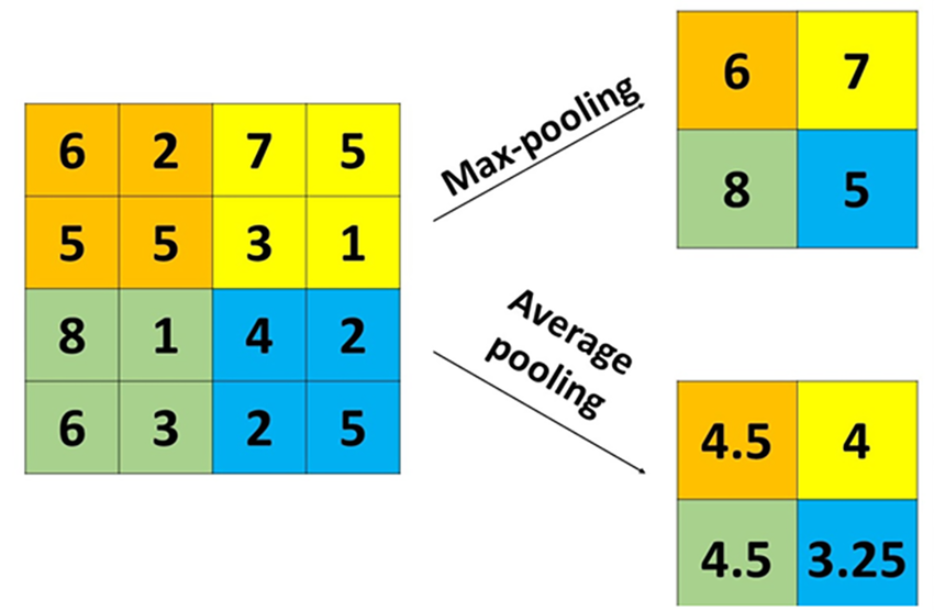
\includegraphics[width=0.70\textwidth]{pooling.png}
    \caption{Il max pooling seleziona la risposta più forte in una regione, enfatizzando la presenza di un pattern, mentre l’average pooling ne fornisce una misura media dell’intensità.}
    \label{fig:convolution_stage}
\end{figure}

Dal punto di vista concettuale, il pooling:
\begin{itemize}
    \item riduce la risoluzione spaziale delle feature map;
    \item diminuisce il costo computazionale dei layer successivi;
    \item introduce una certa invarianza a piccole traslazioni dell’input.
\end{itemize}

Riducendo la dimensionalità delle rappresentazioni intermedie, il pooling contribuisce anche a limitare l’overfitting e a rendere la rete più robusta rispetto a variazioni locali dell’input.

È importante notare che il pooling agisce solo sulle dimensioni spaziali delle feature map e non sulla loro profondità: il numero di feature map rimane invariato.

\subsection{Dimensione delle feature map e numero di parametri}

Si consideri un input tridimensionale di dimensioni
\[
w_{in} \times h_{in} \times d_{in},
\]
dove $w_{in}$ e $h_{in}$ rappresentano le dimensioni spaziali e $d_{in}$ il numero di canali.  
Si considerino inoltre $d_{out}$ kernel convoluzionali di dimensioni
\[
w_k \times h_k \times d_{in},
\]
uno per ciascuna feature map di output, con stride $s$ e padding $p$.

\section{Dimensione della feature map di output}

Le dimensioni spaziali delle feature map di output sono date da:

\[
\highlight{
w_{out} = \frac{w_{in} - w_k + 2p}{s} + 1,
\qquad
h_{out} = \frac{h_{in} - h_k + 2p}{s} + 1.}
\]

Il numero di feature map in output è pari al numero di kernel utilizzati, ovvero $d_{out}$.  
Di conseguenza, l’output del convolutional layer è un tensore di dimensioni:

\[
\highlight{
w_{out} \times h_{out} \times d_{out}.}
\]

\subsubsection{Numero di parametri allenabili}

Il numero di parametri allenabili di un convolutional layer dipende esclusivamente dalle dimensioni dei kernel e dal loro numero, e non dalla dimensione spaziale dell’input.

Ogni kernel contiene:

\[
\highlight{
w_k \cdot h_k \cdot d_{in}}
\]

pesi, e a ciascun kernel è associato un termine di bias.  

Poiché i kernel sono $d_{out}$, il numero totale di parametri allenabili è:

\[
\highlight{
|\theta| = w_k \cdot h_k \cdot d_{in} \cdot d_{out} + d_{out}.}
\]

Questo risultato evidenzia uno dei principali vantaggi delle Convolutional Neural Networks:  
grazie al \textbf{parameter sharing}, il numero di parametri cresce linearmente con il numero di kernel e non con la dimensione dell’input, a differenza delle reti completamente connesse.

\section*{RIEPILOGO}

\begin{tcolorbox}[
    colback=green!5,
    colframe=green!50!black,
    title=Convolutional Neural Networks,
    breakable
]

Le \textbf{Convolutional Neural Networks (CNN)} sono una classe di reti neurali feedforward progettate per elaborare dati strutturati, come immagini, segnali e video.  
Esse sfruttano vincoli architetturali coerenti con la struttura dei dati, ottenendo modelli più efficienti e con migliore capacità di generalizzazione rispetto alle reti completamente connesse.

L’operatore fondamentale delle CNN è la \textbf{convoluzione}, che applica un kernel locale all’input producendo una \textbf{feature map}.  
Nella pratica, viene utilizzata la cross-correlazione, equivalente dal punto di vista dell’apprendimento e più efficiente dal punto di vista computazionale.

Il \textbf{kernel} è un tensore di parametri allenabili che definisce un operatore lineare locale.  
Applicando lo stesso kernel in tutte le posizioni dell’input si realizza il principio di \textbf{parameter sharing}, che consente di rilevare lo stesso pattern indipendentemente dalla sua posizione e riduce drasticamente il numero di parametri.

Ogni valore di una feature map dipende solo da una regione locale dell’input, detta \textbf{receptive field}.  
Questa proprietà, nota come \textbf{sparse connectivity}, permette alle CNN di sfruttare le relazioni locali presenti nei dati e contribuisce all’efficienza del modello.

Un \textbf{convolutional layer} è composto da tre stadi principali:
\begin{itemize}
    \item \textbf{convolution stage}, in cui i kernel vengono applicati all’input;
    \item \textbf{detector stage}, che introduce non linearità tramite funzioni di attivazione (tipicamente ReLU);
    \item \textbf{pooling stage}, che riduce la dimensionalità spaziale delle feature map e introduce invarianza a piccole traslazioni.
\end{itemize}

Il \textbf{padding} consente di controllare la dimensione delle feature map e di preservare l’informazione ai bordi dell’input, mentre lo \textbf{stride} determina di quanto il kernel si sposta sull’input durante la convoluzione.

La dimensione delle feature map di output dipende da input, kernel, padding e stride, mentre il numero di parametri allenabili di un convolutional layer dipende esclusivamente dalle dimensioni dei kernel e dal loro numero, grazie al parameter sharing.

Infine, il \textbf{transfer learning} permette di riutilizzare CNN pre-addestrate su grandi dataset, sfruttando le feature generiche apprese nei layer convoluzionali iniziali per risolvere nuovi compiti con meno dati e minore costo computazionale.

\medskip
\textit{Le CNN rappresentano quindi un’estensione strutturata delle reti neurali classiche, particolarmente efficace per l’elaborazione di dati con struttura spaziale o temporale.}

\end{tcolorbox}


\chapter{Unsupervised Learning}

Nel contesto del \emph{Machine Learning}, si parla di \emph{Unsupervised Learning} quando il processo di apprendimento avviene in assenza di etichette associate ai dati.
Formalmente, è disponibile un insieme di dati di input

\[
\highlight{
\mathcal{D} = \{ \mathbf{x}_n \}_{n=1}^{N},}
\]

ma non sono noti i corrispondenti valori target.

L’obiettivo principale dell’apprendimento non supervisionato non è la predizione di una variabile di uscita, bensì la scoperta di \emph{strutture latenti} nei dati.
Tra i problemi tipici rientrano:
\begin{itemize}
    \item il \textbf{clustering}, ovvero l’individuazione di gruppi omogenei di dati;
    \item la \textbf{modellazione della distribuzione dei dati}, utile anche come fase preliminare a metodi supervisionati;
    \item la \textbf{riduzione della dimensionalità} e l’analisi di variabili latenti.
\end{itemize}

\subsection{Cluster}

Nel contesto dell’apprendimento non supervisionato, un \emph{cluster} è un insieme di dati che presentano caratteristiche simili tra loro e differenti rispetto ai dati appartenenti ad altri gruppi.
L’idea di clustering nasce dall’osservazione che i dati non sono distribuiti in modo uniforme nello spazio delle feature, ma tendono a concentrarsi in regioni ben definite.

Dal punto di vista geometrico, un cluster può essere interpretato come una regione dello spazio in cui la densità dei dati è elevata.
Nel caso dei Gaussian Mixture Models, ciascun cluster è modellato tramite una distribuzione gaussiana, che ne descrive la posizione (media) e la forma (covarianza).

\subsection{Variabili latenti}

Durante il processo di generazione dei dati, ogni osservazione è prodotta da una specifica componente del modello.
Tuttavia, nell’apprendimento non supervisionato, questa informazione non è osservabile direttamente.

Per rappresentare tale informazione nascosta si introducono le \emph{variabili latenti}.
Una variabile latente è una variabile non osservata che influenza la generazione dei dati osservabili.

L’introduzione delle variabili latenti consente di:
\begin{itemize}
    \item modellare esplicitamente l’appartenenza dei dati ai cluster;
    \item passare da un clustering puramente geometrico a un clustering probabilistico;
    \item formulare il problema dell’apprendimento come un problema di inferenza statistica.
\end{itemize}

\section{Gaussian Mixture Models}

Un \emph{Gaussian Mixture Model} (GMM) è un modello probabilistico che assume che i dati osservati siano generati da una combinazione di più distribuzioni gaussiane.
La distribuzione di probabilità complessiva è definita come una combinazione convessa di $K$ componenti gaussiane:

\[
\highlight{
p(\mathbf{x}) = \sum_{k=1}^{K} \pi_k \, \mathcal{N}(\mathbf{x}; \boldsymbol{\mu}_k, \boldsymbol{\Sigma}_k),}
\]

dove:
\begin{itemize}
    \item $\pi_k$ è la probabilità a priori della componente $k$-esima, con $\pi_k \geq 0$ e $\sum_{k=1}^{K} \pi_k = 1$;
    \item $\boldsymbol{\mu}_k$ è il vettore media della $k$-esima gaussiana;
    \item $\boldsymbol{\Sigma}_k$ è la matrice di covarianza associata.
\end{itemize}

Il GMM è un \emph{modello generativo}: descrive esplicitamente il processo attraverso cui i dati vengono prodotti.
In particolare, la generazione di un singolo campione $\mathbf{x}_n$ può essere descritta in due fasi:
\begin{enumerate}
    \item selezione di una componente $k$ secondo la distribuzione discreta definita dai pesi $\{\pi_1, \dots, \pi_K\}$;
    \item generazione del dato $\mathbf{x}_n$ campionando dalla distribuzione gaussiana

    \[
    \highlight{
    \mathcal{N}(\mathbf{x}; \boldsymbol{\mu}_k, \boldsymbol{\Sigma}_k).}
    \]

\end{enumerate}

Nel contesto dell’apprendimento non supervisionato, il problema consiste nello stimare i parametri del modello

\[
\highlight{
\{ \pi_k, \boldsymbol{\mu}_k, \boldsymbol{\Sigma}_k \}_{k=1}^{K}}
\]
a partire dai soli dati osservati $\mathcal{D}$, senza conoscere quale componente gaussiana abbia generato ciascun campione.


\subsection{Generazione dei dati con un Gaussian Mixture Model}

Un \emph{Gaussian Mixture Model} definisce un processo generativo esplicito per i dati osservati.
L’ipotesi fondamentale è che ogni osservazione $\mathbf{x}_n$ sia generata da una tra $K$ distribuzioni gaussiane, selezionata in modo casuale secondo una distribuzione discreta sui componenti.

Il processo generativo può essere descritto come segue:
\begin{enumerate}
    \item si estrae una variabile discreta $k \in \{1, \dots, K\}$ secondo la distribuzione
    \[
    P(k) = \pi_k;
    \]
    \item dato il valore di $k$, si genera il campione $\mathbf{x}_n$ dalla distribuzione gaussiana associata:
    \[
    \mathbf{x}_n \sim \mathcal{N}(\boldsymbol{\mu}_k, \boldsymbol{\Sigma}_k).
    \]
\end{enumerate}

Ripetendo questo processo $N$ volte si ottiene un dataset

\[
\mathcal{D} = \{ \mathbf{x}_1, \dots, \mathbf{x}_N \},
\]

che risulta composto da più gruppi di dati, ciascuno caratterizzato da una propria media, covarianza e peso probabilistico.

Dal punto di vista geometrico, ciascuna componente gaussiana genera un \emph{cluster} con forma ellittica nello spazio delle feature, la cui orientazione e dispersione sono determinate dalla matrice di covarianza $\boldsymbol{\Sigma}_k$.
Un esempio bidimensionale di dati generati da un GMM con due componenti è mostrato in Figura~\ref{fig:GMM}.

\begin{figure}[H]
    \centering
    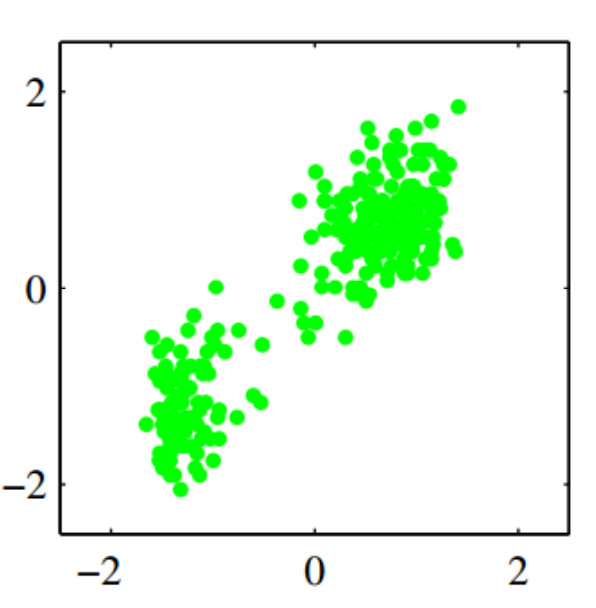
\includegraphics[width=0.6\textwidth]{GMM.png}
    \caption{Esempio di dati generati da un Gaussian Mixture Model con due componenti. Ogni cluster corrisponde a una diversa distribuzione gaussiana con media e covarianza proprie.}
    \label{fig:GMM}
\end{figure}

È importante sottolineare che, nel contesto dell’apprendimento non supervisionato, il dataset osservato contiene esclusivamente i campioni $\mathbf{x}_n$, mentre l’informazione relativa a quale componente gaussiana abbia generato ciascun dato non è osservabile.
Questa informazione nascosta verrà modellata introducendo opportune \emph{variabili latenti}.

\subsection{Introduzione formale delle variabili latenti nel GMM}

Per rendere esplicita l’appartenenza di ciascun dato a un cluster, nel Gaussian Mixture Model si introducono delle variabili latenti discrete.
Per ogni osservazione $\mathbf{x}_n$ si definisce una variabile latente

\[
\highlight{
\mathbf{z}_n = (z_{n1}, \dots, z_{nK})^T,}
\]

dove ciascuna componente $z_{nk}$ è una variabile binaria tale che:

\[
\highlight{
z_{nk} \in \{0,1\}, \qquad \sum_{k=1}^{K} z_{nk} = 1.}
\]

Questa rappresentazione è nota come \emph{codifica 1-out-of-$K$} e garantisce che ogni dato sia associato a una e una sola componente del modello.

La variabile latente $z_{nk} = 1$ indica che il campione $\mathbf{x}_n$ è stato generato dalla $k$-esima distribuzione gaussiana.

\subsection{Distribuzione a priori delle variabili latenti}

Si assume che le variabili latenti siano distribuite secondo una distribuzione categorica parametrizzata dai pesi del modello:

\[
\highlight{
P(z_{nk} = 1) = \pi_k,}
\]

con $\pi_k \geq 0$ e $\sum_{k=1}^{K} \pi_k = 1$.
La distribuzione congiunta della variabile latente $\mathbf{z}_n$ può quindi essere scritta come:

\[
\highlight{
P(\mathbf{z}_n) = \prod_{k=1}^{K} \pi_k^{\, z_{nk}}.}
\]

\subsection{Distribuzione condizionata dei dati}

Dato il valore della variabile latente, la distribuzione del dato osservato è gaussiana:

\[
\highlight{
P(\mathbf{x}_n \mid z_{nk} = 1) = \mathcal{N}(\mathbf{x}_n; \boldsymbol{\mu}_k, \boldsymbol{\Sigma}_k).}
\]

Utilizzando la codifica 1-out-of-$K$, la distribuzione condizionata può essere espressa in forma compatta come:

\[
\highlight{
P(\mathbf{x}_n \mid \mathbf{z}_n)
= \prod_{k=1}^{K}
\mathcal{N}(\mathbf{x}_n; \boldsymbol{\mu}_k, \boldsymbol{\Sigma}_k)^{z_{nk}}.}
\]

\subsection{Distribuzione congiunta e marginale}

Applicando la regola della catena, la distribuzione congiunta delle variabili osservate e latenti è:

\[
\highlight{
P(\mathbf{x}_n, \mathbf{z}_n)
= P(\mathbf{x}_n \mid \mathbf{z}_n) P(\mathbf{z}_n).}
\]

La distribuzione marginale dei dati osservati si ottiene marginalizzando rispetto alle variabili latenti:

\[
\highlight{
P(\mathbf{x}_n) = \sum_{\mathbf{z}_n} P(\mathbf{x}_n, \mathbf{z}_n)
= \sum_{k=1}^{K} \pi_k \, \mathcal{N}(\mathbf{x}_n; \boldsymbol{\mu}_k, \boldsymbol{\Sigma}_k),}
\]

che coincide con l’espressione del Gaussian Mixture Model.

\subsection{Distribuzione a posteriori delle variabili latenti}

Dato un campione osservato $\mathbf{x}_n$, è possibile calcolare la distribuzione a posteriori delle variabili latenti tramite il teorema di Bayes:

\[
\highlight{
\gamma(z_{nk}) \equiv P(z_{nk} = 1 \mid \mathbf{x}_n)
= \frac{\pi_k \, \mathcal{N}(\mathbf{x}_n; \boldsymbol{\mu}_k, \boldsymbol{\Sigma}_k)}
{\sum_{j=1}^{K} \pi_j \, \mathcal{N}(\mathbf{x}_n; \boldsymbol{\mu}_j, \boldsymbol{\Sigma}_j)}.}
\]

La quantità $\gamma(z_{nk})$ rappresenta la \emph{responsabilità} della $k$-esima componente nel generare il dato $\mathbf{x}_n$ ed esprime un’assegnazione probabilistica del campione al cluster.

\paragraph{Interpretazione grafica di un Gaussian Mixture Model}

Un Gaussian Mixture Model descrive i dati come generati da una combinazione
(lineare) di $k$ distribuzioni gaussiane.
Ogni componente gaussiana rappresenta una possibile sorgente dei dati,
caratterizzata da una media e da una matrice di covarianza.

\begin{figure}[H]
\centering
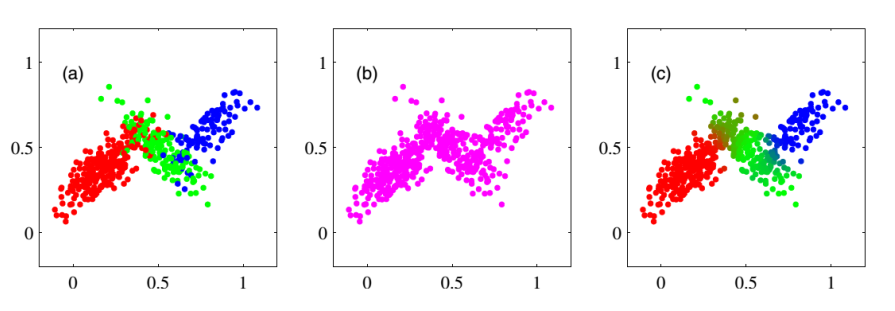
\includegraphics[width=\textwidth]{gmm_interpretation.png}
\caption{Rappresentazione grafica del funzionamento di un Gaussian Mixture Model.
(a) Inizializzazione delle componenti gaussiane.
(b) Distribuzione dei dati senza assegnazione esplicita ai cluster.
(c) Assegnazione probabilistica delle osservazioni alle componenti del modello.}
\end{figure}

La Figura illustra il comportamento di un GMM in tre fasi concettuali.

Nel pannello (a) sono mostrate più componenti gaussiane inizializzate nello
spazio dei dati. Ogni colore rappresenta una diversa gaussiana, definita da
una media e da una covarianza. In questa fase le componenti sono solo ipotesi
sulla struttura dei dati.

Nel pannello (b) si osservano i dati nel loro insieme, senza una suddivisione
esplicita in cluster. A differenza di metodi come il K-means, nel GMM non esiste
un’assegnazione rigida dei punti a un singolo cluster.

Nel pannello (c) è mostrato il risultato del modello appreso: ogni osservazione
è associata probabilisticamente alle diverse componenti gaussiane. I colori
rappresentano la componente con probabilità a posteriori maggiore per ciascun
punto, ma ogni osservazione contribuisce in realtà a tutte le componenti in
misura diversa.

\subsubsection{Ruolo del parametro $k$}

Nel Gaussian Mixture Model, il parametro $k$ indica il numero di componenti
gaussiane che costituiscono il modello.
A differenza del K-means, in cui $k$ rappresenta il numero di cluster rigidi,
nel GMM $k$ rappresenta il numero di distribuzioni probabilistiche utilizzate
per modellare i dati.

Ogni componente gaussiana non corrisponde necessariamente a un cluster ben
separato, ma contribuisce alla distribuzione complessiva dei dati.
Valori diversi di $k$ permettono di modellare strutture più o meno complesse:
\begin{itemize}
\item un valore di $k$ piccolo produce un modello più semplice;
\item un valore di $k$ grande consente di approssimare distribuzioni più complesse,
ma aumenta il rischio di overfitting.
\end{itemize}

Il valore di $k$ è quindi un iperparametro del modello e deve essere scelto
in base al compromesso tra capacità di rappresentazione e generalizzazione.



\section{K-means Clustering}

L’algoritmo \emph{K-means} è uno dei metodi più semplici e diffusi per il clustering non supervisionato.
Dato un insieme di dati
\[
\mathcal{D} = \{ \mathbf{x}_n \}_{n=1}^{N}
\]
e un numero fissato di cluster $K$, l’obiettivo di K-means è suddividere i dati in $K$ gruppi minimizzando la distanza tra ciascun punto e il centro del cluster a cui è assegnato.

\subsection{Obiettivo dell’algoritmo}

K-means mira a minimizzare la seguente funzione obiettivo:

\[
\highlight{
J = \sum_{n=1}^{N} \sum_{k=1}^{K} r_{nk} \, \lVert \mathbf{x}_n - \boldsymbol{\mu}_k \rVert^2,}
\]

dove:
\begin{itemize}
    \item $\boldsymbol{\mu}_k$ è il centroide del cluster $k$;
    \item $r_{nk} \in \{0,1\}$ è una variabile di assegnazione tale che $r_{nk}=1$ se il punto $\mathbf{x}_n$ appartiene al cluster $k$ e $0$ altrimenti;
    \item per ogni $n$, vale il vincolo $\sum_{k=1}^{K} r_{nk} = 1$.
\end{itemize}

Questo formalizza un \emph{hard clustering}: ogni dato appartiene a un solo cluster.

\subsection{Algoritmo K-means}

L’algoritmo procede in modo iterativo alternando due fasi:

\paragraph{Fase di assegnazione}
Dato un insieme corrente di centroidi $\{\boldsymbol{\mu}_k\}$, ogni punto viene assegnato al cluster il cui centroide è più vicino:
\[
r_{nk} =
\begin{cases}
1 & \text{se } k = \arg\min_j \lVert \mathbf{x}_n - \boldsymbol{\mu}_j \rVert^2, \\
0 & \text{altrimenti}.
\end{cases}
\]

\paragraph{Fase di aggiornamento}
Una volta fissate le assegnazioni, i centroidi vengono ricalcolati come media dei punti appartenenti al cluster:

\[
\highlight{
\boldsymbol{\mu}_k = \frac{1}{N_k} \sum_{n=1}^{N} r_{nk} \, \mathbf{x}_n,
\qquad
N_k = \sum_{n=1}^{N} r_{nk}.}
\]

Queste due fasi vengono ripetute fino a convergenza, ovvero fino a quando le assegnazioni non cambiano più oppure la funzione obiettivo non diminuisce ulteriormente.

\subsection{Interpretazione geometrica}

La Figura~\ref{fig:k-means} mostra l’evoluzione dell’algoritmo K-means nel caso bidimensionale con $K=2$:
a partire da centroidi iniziali arbitrari, le assegnazioni e i centroidi vengono aggiornati iterativamente fino alla convergenza.

\begin{figure}[H]
    \centering
    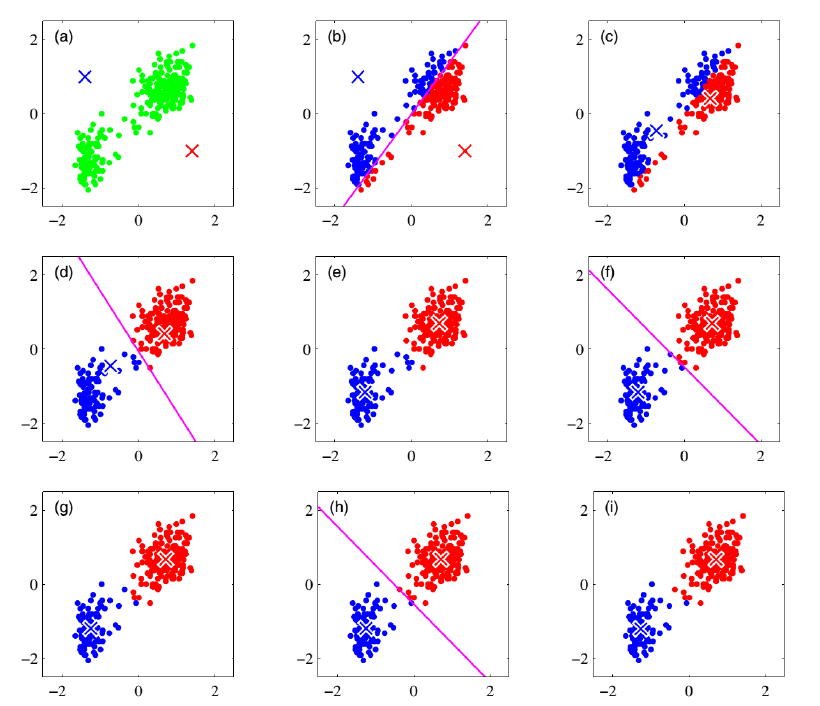
\includegraphics[width=0.9\textwidth]{k-means.png}
    \caption{Evoluzione dell’algoritmo K-means. I punti sono assegnati ai cluster in base alla distanza dal centroide corrente; le linee indicano i confini di decisione. Le croci rappresentano i centroidi, che vengono aggiornati a ogni iterazione fino alla convergenza.}
    \label{fig:k-means}
\end{figure}

Dal punto di vista geometrico, K-means costruisce una partizione dello spazio in regioni di Voronoi, ciascuna associata a un centroide.
I confini tra i cluster sono iperpiani determinati dalla distanza euclidea dai centroidi.


\subsubsection{Osservazioni}

K-means è un algoritmo semplice ed efficiente, ma presenta alcune limitazioni:
\begin{itemize}
    \item il numero di cluster $K$ deve essere fissato a priori;
    \item il risultato dipende fortemente dall’inizializzazione dei centroidi;
    \item il clustering è basato esclusivamente sulla distanza euclidea;
    \item i cluster ottenuti hanno forma approssimativamente sferica.
\end{itemize}

Queste limitazioni motivano l’introduzione di modelli probabilistici più generali, come i Gaussian Mixture Models, e di algoritmi di stima più flessibili, come l’Expectation Maximization.

\section{Expectation Maximization (EM)}

Nel caso dei Gaussian Mixture Models, il problema dell’apprendimento consiste nello stimare i parametri

\[
\highlight{
\Theta = \{ \pi_k, \boldsymbol{\mu}_k, \boldsymbol{\Sigma}_k \}_{k=1}^{K}}
\]

a partire da un insieme di dati osservati

\[
\highlight{
\mathcal{D} = \{ \mathbf{x}_n \}_{n=1}^{N},}
\]

in presenza di variabili latenti non osservabili $\mathbf{z}_n$.

\subsection{Massima verosimiglianza con variabili latenti}

L’obiettivo è massimizzare la log-verosimiglianza dei dati osservati:

\[
\highlight{
\ln p(\mathcal{D} \mid \Theta)
= \sum_{n=1}^{N} \ln \left( \sum_{k=1}^{K}
\pi_k \, \mathcal{N}(\mathbf{x}_n; \boldsymbol{\mu}_k, \boldsymbol{\Sigma}_k) \right).}
\]

La presenza della somma all’interno del logaritmo rende la massimizzazione diretta di questa funzione un problema non banale.
Questa difficoltà è dovuta al fatto che le variabili latenti $\mathbf{z}_n$, che indicano quale componente abbia generato ciascun dato, non sono osservabili.

\subsection{Idea dell’algoritmo EM}

L’algoritmo \emph{Expectation Maximization} affronta il problema alternando due fasi:
\begin{itemize}
    \item una fase di \textbf{stima} delle variabili latenti, data una stima corrente dei parametri;
    \item una fase di \textbf{aggiornamento} dei parametri, data la distribuzione stimata delle variabili latenti.
\end{itemize}

L’algoritmo procede quindi per ottimizzazione iterativa, migliorando la log-verosimiglianza dei dati a ogni iterazione.

\subsection{E-step (Expectation step)}

Dato un insieme corrente di parametri $\Theta^{(t)}$, si calcola la distribuzione a posteriori delle variabili latenti:

\[
\highlight{
\gamma(z_{nk})^{(t+1)} \equiv
P(z_{nk} = 1 \mid \mathbf{x}_n, \Theta^{(t)})
=
\frac{\pi_k^{(t)} \, \mathcal{N}(\mathbf{x}_n; \boldsymbol{\mu}_k^{(t)}, \boldsymbol{\Sigma}_k^{(t)})}
{\sum_{j=1}^{K} \pi_j^{(t)} \, \mathcal{N}(\mathbf{x}_n; \boldsymbol{\mu}_j^{(t)}, \boldsymbol{\Sigma}_j^{(t)})}.}
\]

Questa quantità rappresenta la \emph{responsabilità} della $k$-esima componente nella generazione del dato $\mathbf{x}_n$.
A differenza di K-means, l’assegnazione ai cluster è ora \emph{soft} e probabilistica.

\subsection{M-step (Maximization step)}

Utilizzando le responsabilità $\gamma(z_{nk})^{(t+1)}$, si aggiornano i parametri del modello:

\paragraph{Aggiornamento delle medie}
\[
\boldsymbol{\mu}_k^{(t+1)} =
\frac{1}{N_k}
\sum_{n=1}^{N}
\gamma(z_{nk})^{(t+1)} \, \mathbf{x}_n,
\qquad
N_k = \sum_{n=1}^{N} \gamma(z_{nk})^{(t+1)}.
\]

\paragraph{Aggiornamento delle covarianze}
\[
\boldsymbol{\Sigma}_k^{(t+1)} =
\frac{1}{N_k}
\sum_{n=1}^{N}
\gamma(z_{nk})^{(t+1)}
(\mathbf{x}_n - \boldsymbol{\mu}_k^{(t+1)})
(\mathbf{x}_n - \boldsymbol{\mu}_k^{(t+1)})^T.
\]

\paragraph{Aggiornamento dei pesi}
\[
\pi_k^{(t+1)} = \frac{N_k}{N}.
\]

\subsection{Algoritmo EM}

L’algoritmo EM può essere riassunto come segue:
\begin{enumerate}
    \item inizializzazione dei parametri $\Theta^{(0)}$;
    \item ripetizione alternata di E-step e M-step;
    \item arresto quando la log-verosimiglianza converge o dopo un numero prefissato di iterazioni.
\end{enumerate}

L’algoritmo converge a un massimo locale della log-verosimiglianza dei dati osservati.

\subsection{Relazione con K-means}

L’algoritmo EM per i Gaussian Mixture Models può essere visto come una generalizzazione probabilistica di K-means.
In particolare:
\begin{itemize}
    \item K-means utilizza assegnazioni hard, mentre EM utilizza assegnazioni soft;
    \item K-means assume cluster sferici e varianze identiche;
    \item EM permette cluster ellittici e di diversa dispersione.
\end{itemize}

\subsection{Interpretazione dell’algoritmo EM}

Il comportamento dell’algoritmo EM può essere compreso osservando l’evoluzione iterativa delle distribuzioni gaussiane stimate.
La Figura~\ref{fig:em} mostra un esempio bidimensionale di apprendimento di un GMM con due componenti.

\begin{figure}[H]
    \centering
    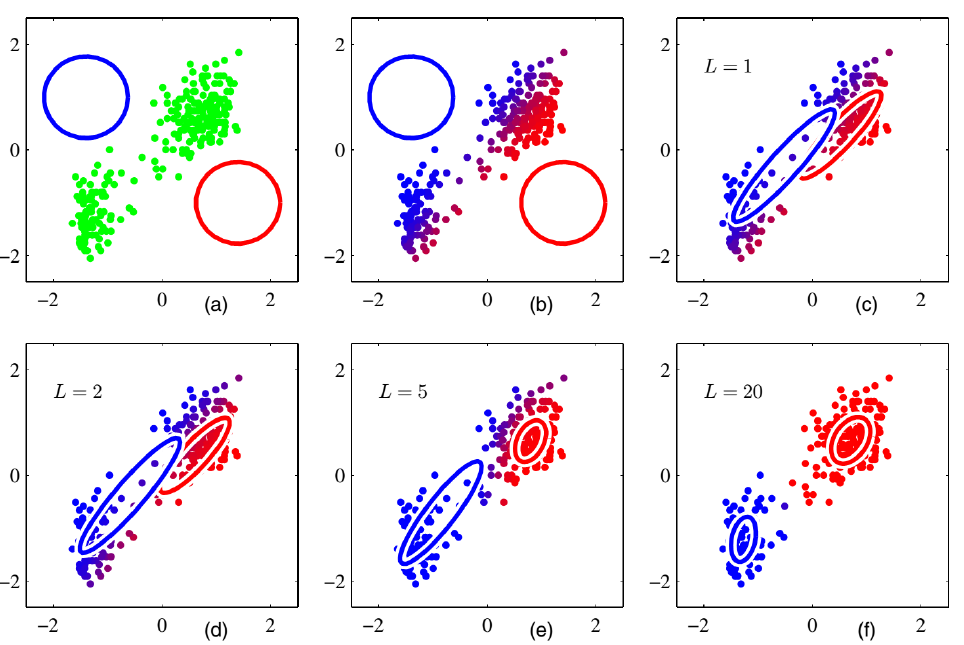
\includegraphics[width=0.95\textwidth]{em.png}
    \caption{Evoluzione dell’algoritmo EM per un Gaussian Mixture Model con due componenti. Le ellissi rappresentano le curve di livello delle distribuzioni gaussiane stimate. Il numero $L$ indica l’iterazione dell’algoritmo.}
    \label{fig:em}
\end{figure}

Nella fase iniziale (Figura~(a)), i parametri del modello sono inizializzati in modo approssimativo: le gaussiane non riflettono ancora la reale struttura dei dati.
Durante le prime iterazioni (Figure~(b) e (c)), l’algoritmo EM alterna:
\begin{itemize}
    \item una stima probabilistica dell’appartenenza dei punti ai cluster (E-step);
    \item un aggiornamento dei parametri delle gaussiane (M-step).
\end{itemize}

A ogni iterazione $L$, le ellissi si deformano e si spostano per adattarsi progressivamente alla distribuzione dei dati.
In particolare:
\begin{itemize}
    \item le medie si muovono verso le regioni di maggiore densità;
    \item le covarianze catturano orientazione e dispersione dei cluster;
    \item le assegnazioni diventano via via più nette.
\end{itemize}

Dopo un numero sufficiente di iterazioni (Figure~(d), (e) e (f)), il modello converge a una configurazione stabile in cui ciascuna componente gaussiana descrive correttamente uno dei cluster presenti nei dati.

Questa rappresentazione evidenzia una differenza fondamentale rispetto a K-means:
mentre K-means aggiorna solo i centroidi e produce cluster sferici,
EM apprende anche la forma, l’orientazione e la dispersione dei cluster attraverso le matrici di covarianza.

\section{General Expectation Maximization Problem}

L’algoritmo Expectation Maximization non è limitato ai Gaussian Mixture Models, ma rappresenta un metodo generale per la stima dei parametri di modelli probabilistici in presenza di variabili latenti.

\subsection{Definizione del problema}

Si consideri:
\begin{itemize}
    \item un insieme di dati osservati
    \[
    X = \{ \mathbf{x}_1, \dots, \mathbf{x}_N \};
    \]
    \item un insieme di variabili latenti non osservate
    \[
    Z = \{ \mathbf{z}_1, \dots, \mathbf{z}_N \};
    \]
    \item un modello probabilistico parametrizzato
    \[
    p(\mathbf{y} \mid \boldsymbol{\theta}),
    \quad \text{dove } \mathbf{y}_n = (\mathbf{x}_n, \mathbf{z}_n)
    \]
    rappresenta il \emph{dato completo}.
\end{itemize}

L’obiettivo è determinare il valore dei parametri
\[
\boldsymbol{\theta}^*
\]
che massimizza la log-verosimiglianza dei dati osservati:
\[
\boldsymbol{\theta}^* = \arg\max_{\boldsymbol{\theta}} \ln p(X \mid \boldsymbol{\theta}).
\]

Poiché le variabili latenti $Z$ non sono osservabili, la massimizzazione diretta della verosimiglianza risulta in generale complessa o intrattabile.

\subsection{Funzione ausiliaria $Q$}

L’algoritmo EM introduce una funzione ausiliaria

\[
\highlight{
Q(\boldsymbol{\theta}' \mid \boldsymbol{\theta})
= \mathbb{E}_{Z \mid X, \boldsymbol{\theta}}
\left[ \ln p(X, Z \mid \boldsymbol{\theta}') \right],}
\]

che rappresenta il valore atteso della log-verosimiglianza del dato completo, calcolato rispetto alla distribuzione a posteriori delle variabili latenti, data la stima corrente dei parametri $\boldsymbol{\theta}$.

\subsection{Algoritmo EM generale}

L’algoritmo EM procede iterativamente secondo i seguenti passi:

\paragraph{E-step (Expectation)}
Dato il valore corrente dei parametri $\boldsymbol{\theta}^{(t)}$, si calcola la distribuzione a posteriori delle variabili latenti e la funzione:

\[
\highlight{
Q(\boldsymbol{\theta}' \mid \boldsymbol{\theta}^{(t)})
= \mathbb{E}_{Z \mid X, \boldsymbol{\theta}^{(t)}}
\left[ \ln p(X, Z \mid \boldsymbol{\theta}') \right].}
\]

\paragraph{M-step (Maximization)}
Si aggiornano i parametri massimizzando la funzione $Q$:

\[
\highlight{
\boldsymbol{\theta}^{(t+1)} =
\arg\max_{\boldsymbol{\theta}'} Q(\boldsymbol{\theta}' \mid \boldsymbol{\theta}^{(t)}).}
\]

Questi due passi vengono ripetuti fino a convergenza.

\subsection{Proprietà dell’algoritmo EM}

L’algoritmo EM presenta le seguenti proprietà generali:
\begin{itemize}
    \item la log-verosimiglianza dei dati osservati non diminuisce a ogni iterazione;
    \item la convergenza è garantita verso un massimo locale;
    \item la qualità della soluzione dipende dall’inizializzazione dei parametri;
    \item il metodo è applicabile a un’ampia classe di modelli con variabili latenti.
\end{itemize}

\subsection{Applicazioni}

Il framework generale di EM trova applicazione in numerosi contesti, tra cui:
\begin{itemize}
    \item clustering non supervisionato;
    \item Gaussian Mixture Models;
    \item Hidden Markov Models;
    \item Bayesian Networks;
    \item modelli con variabili latenti continue o discrete.
\end{itemize}


\section*{RIEPILOGO}
\begin{tcolorbox}[
    colback=green!5,
    colframe=green!60!black,
    title=\textbf{Unsupervised learning},
    fonttitle=\bfseries,
    coltitle=black,
    boxed title style={
        colback=green!60!black,
        colframe=green!60!black
    }
]

L'\textbf{apprendimento non supervisionato} si applica a contesti in cui sono disponibili solo i dati di input, senza etichette associate. L'obiettivo è individuare strutture latenti nei dati, come cluster o pattern statistici, direttamente a partire dalle osservazioni.

I \textbf{Gaussian Mixture Models (GMM)} sono modelli probabilistici generativi che descrivono i dati come generati da una combinazione di distribuzioni gaussiane. Ogni componente del modello rappresenta un cluster ed è caratterizzata da una media, una matrice di covarianza e una probabilità a priori.

Per modellare l'appartenenza dei dati ai cluster si introducono \textbf{variabili latenti}, che indicano quale componente gaussiana ha generato ciascun campione. Queste variabili non sono osservabili e devono essere inferite insieme ai parametri del modello.

L'algoritmo \textbf{K-means} fornisce una soluzione semplice al problema del clustering basata su assegnazioni hard e distanza euclidea. Sebbene efficiente, è limitato a cluster sferici, è sensibile all'inizializzazione e non fornisce una modellazione probabilistica.

L'\textbf{Expectation Maximization (EM)} generalizza K-means introducendo assegnazioni soft e una formulazione probabilistica. L'algoritmo alterna una fase di stima delle variabili latenti (E-step) e una fase di aggiornamento dei parametri del modello (M-step), garantendo la non diminuzione della log-verosimiglianza e la convergenza a un massimo locale.

Infine, EM rappresenta un \textbf{metodo generale di inferenza} applicabile a un'ampia classe di modelli con variabili latenti, come Gaussian Mixture Models, Hidden Markov Models e Bayesian Networks.

\end{tcolorbox}


\chapter{Dimensionally reduction}

\section{Variabili latenti}

Nei problemi di riduzione della dimensionalità, i dati osservati sono spesso rappresentati in spazi ad alta dimensionalità. Tuttavia, la dimensionalità dello spazio di rappresentazione non coincide necessariamente con il numero di gradi di libertà che descrivono le variazioni significative dei dati.

Le \emph{variabili latenti} rappresentano tali gradi di libertà nascosti, non direttamente osservabili, che generano i dati osservati. Sebbene ogni campione sia descritto da un vettore ad alta dimensionalità

\[
\highlight{
\mathbf{x}_n \in \mathbb{R}^d,}
\]

la variabilità effettiva dei dati può essere spiegata da un numero molto inferiore di parametri.

Un esempio semplice è costituito da un insieme di immagini ottenute ruotando un singolo prototipo. 
In questo caso, ogni immagine è rappresentata da un vettore ad alta dimensionalità, ma tutte le variazioni osservate dipendono 
da un unico parametro, l'angolo di rotazione. Il dataset presenta quindi un solo grado di libertà.

\begin{figure}[h]
    \centering
    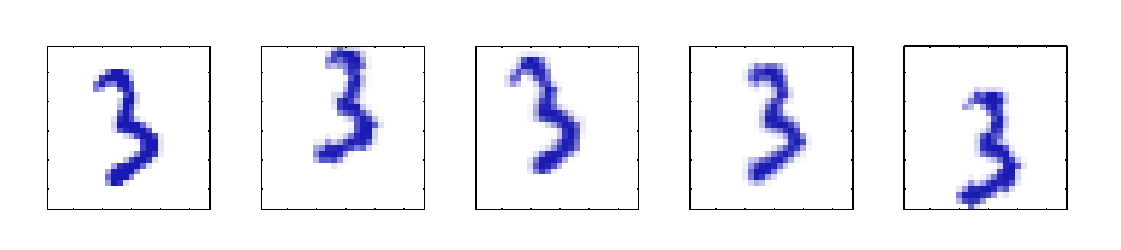
\includegraphics[width=0.9\textwidth]{3.png}
    \caption{Esempio di immagini della stessa cifra scritta a mano. 
    Sebbene ogni immagine sia rappresentata in uno spazio ad alta dimensionalità, 
    le variazioni osservate sono riconducibili a un numero ridotto di gradi di libertà 
    (variabili latenti), come rotazioni, traslazioni e differenze di stile.}
    \label{fig:3}
\end{figure}

Un ulteriore esempio è dato da un insieme di immagini RGB di dimensione $100 \times 100$, ottenute mediante trasformazioni 
geometriche di una singola immagine. Sebbene ogni immagine appartenga a uno spazio di dimensione $30{,}000$, le trasformazioni 
applicate (traslazioni bidimensionali e rotazione) introducono soltanto tre gradi di libertà. 
Questo evidenzia come lo spazio dei dati sia molto più grande dello spazio delle variazioni effettive.

\section{Manifold dei dati}

Quando i dati presentano una struttura interna, essi non occupano uniformemente l'intero spazio di rappresentazione, 
ma si distribuiscono su una regione a dimensionalità inferiore. Questa regione viene detta \emph{manifold}.

\begin{figure}[H]
    \centering
    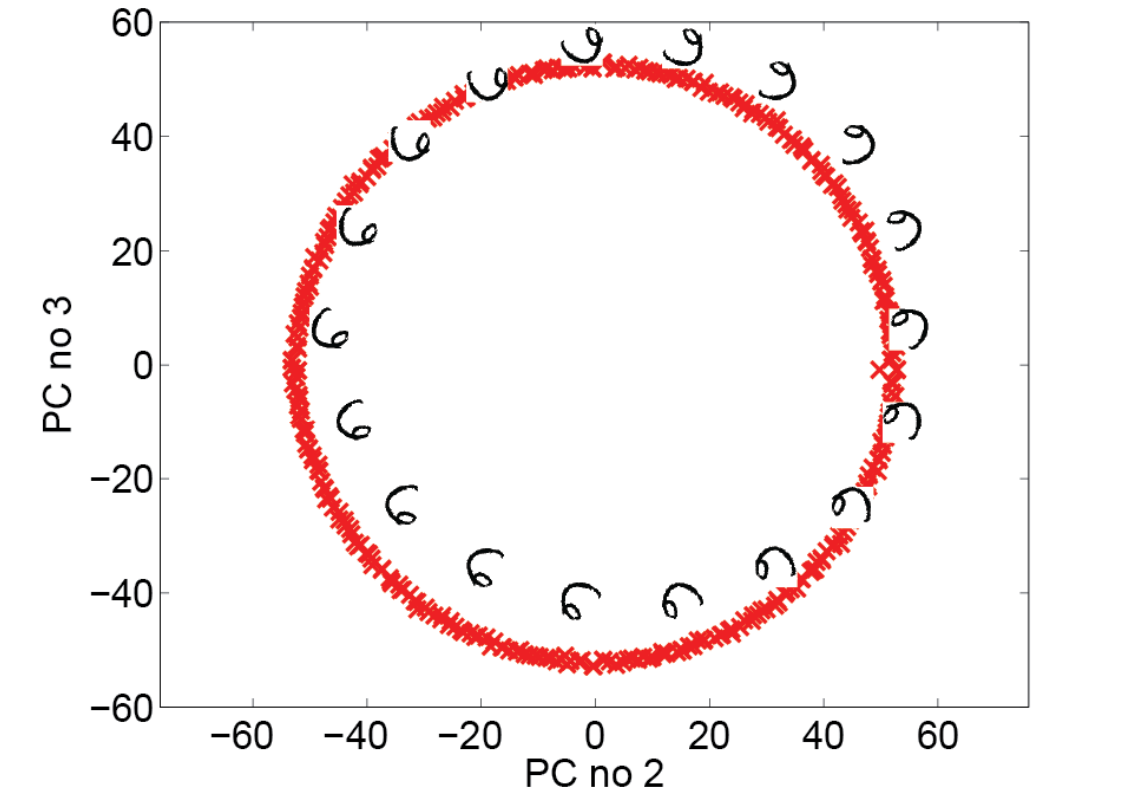
\includegraphics[width=0.7\textwidth]{manifold.png}
    \caption{Rappresentazione del manifold dei dati ottenuta proiettando immagini della stessa cifra sulle componenti principali PC2 e PC3.}
    \label{fig:manifold}
\end{figure}


La nozione di manifold può essere visualizzata proiettando i dati in uno spazio a dimensionalità ridotta. 
In Figura~\ref{fig:manifold} sono riportate le proiezioni di immagini della stessa cifra scritta a mano sulle componenti principali seconda e terza.
Sebbene lo spazio di rappresentazione sia bidimensionale, i dati non occupano l'intero piano, ma si distribuiscono lungo una 
struttura continua e chiusa. Questa struttura rappresenta il manifold su cui giacciono i dati: 
una varietà a dimensionalità inferiore che riflette i gradi di libertà effettivi del dataset.

In questo caso, la disposizione circolare dei punti è coerente con una variazione continua di un singolo fattore latente, 
come ad esempio la rotazione del prototipo. La figura mostra quindi come dati ad alta dimensionalità possano essere descritti 
efficacemente come campioni di un manifold a bassa dimensionalità immerso in uno spazio di dimensione maggiore.

Per dati dotati di struttura, il numero di distorsioni o trasformazioni rilevanti è inferiore al numero di dimensioni dello spazio dei dati. 
Di conseguenza, i campioni appartengono a un manifold a dimensionalità ridotta.

\section{Principal Component Analysis}

La \emph{Principal Component Analysis} (PCA) è una delle tecniche più utilizzate per la riduzione della dimensionalità. L'obiettivo della PCA è individuare una rappresentazione a dimensione ridotta dei dati che preservi il più possibile la loro struttura, mantenendo le variazioni più significative.

La PCA viene comunemente impiegata per:
\begin{itemize}
    \item riduzione della dimensionalità;
    \item compressione dei dati (con perdita di informazione controllata);
    \item visualizzazione di dati ad alta dimensionalità;
    \item estrazione di caratteristiche rilevanti.
\end{itemize}

Dal punto di vista geometrico, la PCA ricerca nuove direzioni nello spazio dei dati lungo le quali la variabilità dei campioni è massima. 
Proiettando i dati su tali direzioni, è possibile ottenere una rappresentazione compatta che approssima il manifold su cui i dati giacciono.

\subsection{Centratura dei dati e matrice di covarianza}

Per poter misurare correttamente la varianza dei dati proiettati, è necessario considerare dati centrati rispetto alla loro media.

La media del dataset è definita come
\[
\bar{\mathbf{x}} = \frac{1}{N} \sum_{n=1}^{N} \mathbf{x}_n.
\]

A partire da essa si costruisce la matrice dei dati centrati
\[
\mathbf{X} =
\begin{bmatrix}
(\mathbf{x}_1 - \bar{\mathbf{x}})^T \\
\vdots \\
(\mathbf{x}_n - \bar{\mathbf{x}})^T \\
\vdots \\
(\mathbf{x}_N - \bar{\mathbf{x}})^T
\end{bmatrix}
\in \mathbb{R}^{N \times d}.
\]

La matrice di covarianza del dataset è quindi definita come
\[
\mathbf{S} = \frac{1}{N} \sum_{n=1}^{N} (\mathbf{x}_n - \bar{\mathbf{x}})(\mathbf{x}_n - \bar{\mathbf{x}})^T
= \frac{1}{N} \mathbf{X}^T \mathbf{X}.
\]

La matrice di covarianza $\mathbf{S}$ descrive come le diverse componenti dei dati variano congiuntamente ed è l'oggetto centrale su cui si basa la PCA.

\subsection{Massimizzazione della varianza}

Si consideri la proiezione dei dati centrati lungo una direzione unitaria
\[
\mathbf{u}_1 \in \mathbb{R}^d, \qquad \mathbf{u}_1^T \mathbf{u}_1 = 1.
\]
La proiezione del campione $\mathbf{x}_n$ è data da $\mathbf{u}_1^T \mathbf{x}_n$, mentre la proiezione della media è $\mathbf{u}_1^T \bar{\mathbf{x}}$.

La varianza dei dati proiettati può essere scritta come

\[
\highlight{
\frac{1}{N} \sum_{n=1}^{N} \left( \mathbf{u}_1^T \mathbf{x}_n - \mathbf{u}_1^T \bar{\mathbf{x}} \right)^2
= \mathbf{u}_1^T \mathbf{S} \mathbf{u}_1,}
\]

dove $\mathbf{S}$ è la matrice di covarianza del dataset.

Il problema della PCA consiste quindi nel massimizzare la varianza dei dati proiettati, imponendo che la direzione di proiezione 
abbia norma unitaria:

\[
\highlight{
\max_{\mathbf{u}_1} \; \mathbf{u}_1^T \mathbf{S} \mathbf{u}_1
\qquad \text{soggetto a} \qquad
\mathbf{u}_1^T \mathbf{u}_1 = 1.}
\]

Questo problema vincolato può essere risolto introducendo un moltiplicatore di Lagrange $\lambda_1$ e considerando la funzione

\[
\highlight{
\mathcal{L}(\mathbf{u}_1, \lambda_1)
= \mathbf{u}_1^T \mathbf{S} \mathbf{u}_1
+ \lambda_1 \left( 1 - \mathbf{u}_1^T \mathbf{u}_1 \right).}
\]

Imponendo l'annullamento della derivata rispetto a $\mathbf{u}_1$ si ottiene
\[
\mathbf{S} \mathbf{u}_1 = \lambda_1 \mathbf{u}_1.
\]
Pertanto, la direzione che massimizza la varianza è un autovettore della matrice di covarianza.

Moltiplicando a sinistra per $\mathbf{u}_1^T$ e usando il vincolo di normalizzazione, si ha
\[
\mathbf{u}_1^T \mathbf{S} \mathbf{u}_1 = \lambda_1,
\]
che rappresenta la varianza dei dati proiettati lungo la direzione $\mathbf{u}_1$.

La varianza è massima quando $\mathbf{u}_1$ è l'autovettore associato al massimo autovalore $\lambda_1$ della matrice di covarianza.
Questa direzione prende il nome di \emph{prima componente principale}.

\section{PCA come minimizzazione dell'errore di ricostruzione}

Si consideri una base ortonormale completa dello spazio dei dati
\[
\{ \mathbf{u}_i \}_{i=1}^{d}, \qquad \mathbf{u}_i^T \mathbf{u}_j = \delta_{ij},
\]
dove $\delta_{ij}$ è il delta di Kronecker. Ogni campione $\mathbf{x}_n$ può essere espresso come combinazione lineare di tali vettori:
\[
\mathbf{x}_n = \sum_{i=1}^{d} \alpha_{ni} \mathbf{u}_i.
\]
Grazie all'ortonormalità della base, i coefficienti sono dati da
\[
\alpha_{ni} = \mathbf{x}_n^T \mathbf{u}_i,
\]
e quindi
\[
\mathbf{x}_n = \sum_{i=1}^{d} (\mathbf{x}_n^T \mathbf{u}_i)\,\mathbf{u}_i.
\]

L'obiettivo della riduzione della dimensionalità è approssimare ogni campione $\mathbf{x}_n$ utilizzando solo $m < d$ componenti. 
L'approssimazione può essere scritta come

\[
\highlight{
\tilde{\mathbf{x}}_n
= \sum_{i=1}^{m} z_{ni} \mathbf{u}_i
+ \sum_{i=m+1}^{d} b_i \mathbf{u}_i,}
\]

dove $z_{ni}$ sono coefficienti dipendenti dal campione, mentre $b_i$ sono termini costanti, indipendenti da $n$.

\begin{figure}[H]
    \centering
    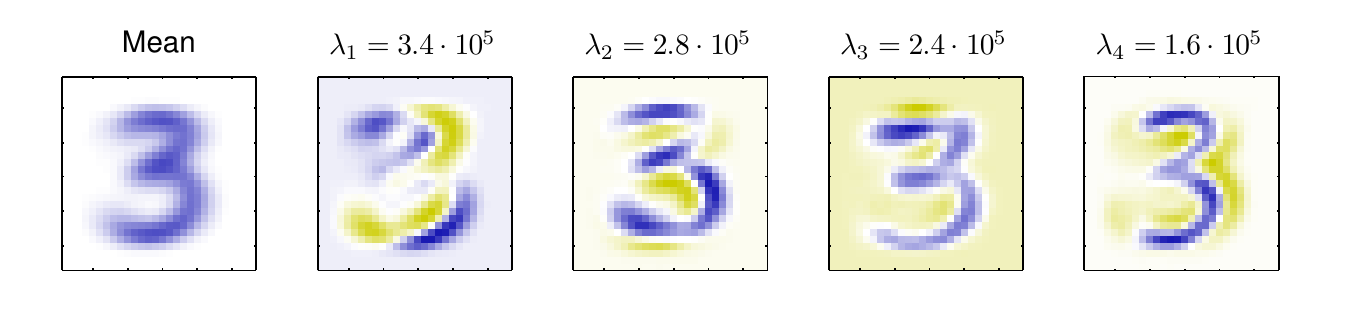
\includegraphics[width=0.7\textwidth]{PCA1.png}
    \caption{Media del dataset e prime componenti principali ottenute tramite PCA. 
            Ogni componente principale corrisponde a un autovettore della matrice di covarianza 
            ed evidenzia una direzione di variazione significativa nei dati. 
            Le componenti sono ordinate in base al valore decrescente dell’autovalore associato, 
            che misura la varianza spiegata lungo ciascuna direzione.}
    \label{fig:PCA1}
\end{figure}

L'errore di approssimazione viene misurato tramite l'errore quadratico medio (MSE):

\[
\highlight{
J = \frac{1}{N} \sum_{n=1}^{N} \left\| \mathbf{x}_n - \tilde{\mathbf{x}}_n \right\|^2.}
\]

Minimizzando $J$ rispetto ai coefficienti $z_{ni}$ e ai termini $b_i$, si ottiene
\[
z_{ni} = \mathbf{x}_n^T \mathbf{u}_i, \qquad i = 1, \ldots, m,
\]
\[
b_i = \bar{\mathbf{x}}^T \mathbf{u}_i, \qquad i = m+1, \ldots, d.
\]

Sostituendo tali espressioni, l'errore di ricostruzione diventa

\[
\highlight{
\mathbf{x}_n - \tilde{\mathbf{x}}_n
= \sum_{i=m+1}^{d} \left[ (\mathbf{x}_n - \bar{\mathbf{x}})^T \mathbf{u}_i \right] \mathbf{u}_i,}
\]

e l'errore quadratico medio complessivo risulta

\[
\highlight{
J = \sum_{i=m+1}^{d} \mathbf{u}_i^T \mathbf{S} \mathbf{u}_i,}
\]
dove $\mathbf{S}$ è la matrice di covarianza del dataset.

La minimizzazione dell'errore $J$ sotto il vincolo di normalizzazione $\mathbf{u}_i^T \mathbf{u}_i = 1$ porta all'equazione agli autovalori

\[
\highlight{
\mathbf{S} \mathbf{u}_i = \lambda_i \mathbf{u}_i.}
\]

\begin{figure}[H]
    \centering
    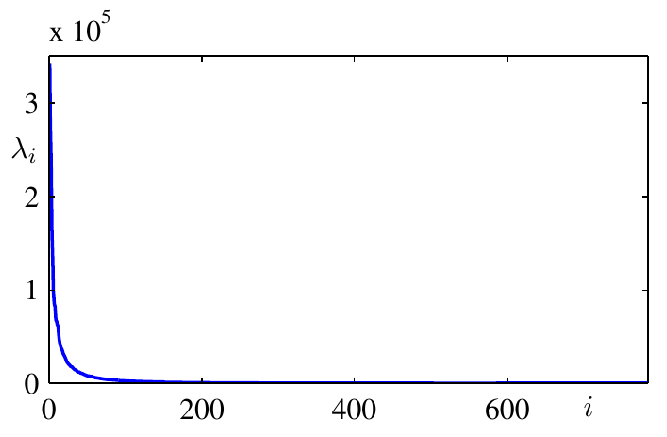
\includegraphics[width=0.7\textwidth]{PCA2.png}
    \caption{Spettro degli autovalori della matrice di covarianza. 
            Ogni autovalore $\lambda_i$ rappresenta la varianza dei dati lungo la corrispondente componente principale. 
            La rapida decrescita degli autovalori indica che gran parte della variabilità del dataset è concentrata nelle prime 
            componenti.}
    \label{fig:PCA2}
\end{figure}

L'errore di ricostruzione minimo è dato dalla somma degli autovalori associati alle componenti scartate:

\[
\highlight{
J = \sum_{i=m+1}^{d} \lambda_i.}
\]

Pertanto, l'errore è minimizzato scegliendo come componenti principali gli autovettori associati ai $m$ autovalori maggiori 
della matrice di covarianza. Questo dimostra che la massimizzazione della varianza e la minimizzazione dell'errore di 
ricostruzione sono formulazioni equivalenti della PCA.

\begin{figure}[H]
    \centering
    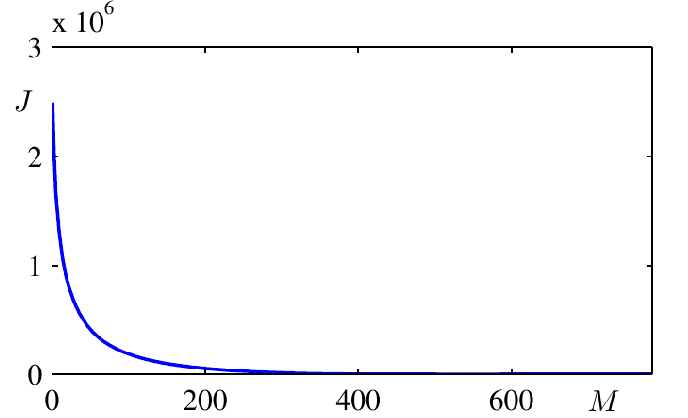
\includegraphics[width=0.7\textwidth]{PCA3.png}
    \caption{Andamento dell’errore di ricostruzione in funzione del numero di componenti principali mantenute. 
            L’errore è pari alla somma degli autovalori scartati e diminuisce rapidamente all’aumentare delle componenti incluse, 
            mostrando l’equivalenza tra massimizzazione della varianza e minimizzazione dell’errore di ricostruzione nella PCA.}
    \label{fig:PCA3}
\end{figure}


\section{Algoritmi per la PCA}

Una volta formulato il problema della PCA, le componenti principali possono essere calcolate in diversi modi equivalenti, che differiscono principalmente per efficienza computazionale.

\begin{enumerate}
    \item \textbf{Autodecomposizione completa della matrice di covarianza.}  
    Si calcola la matrice di covarianza
    \[
    \mathbf{S} = \frac{1}{N} \mathbf{X}^T \mathbf{X},
    \]
    e se ne determinano tutti gli autovalori e gli autovettori. Questo approccio è concettualmente semplice, ma computazionalmente costoso quando la dimensionalità $d$ è elevata.
    
    \item \textbf{Autodecomposizione parziale.}  
    In molti casi è sufficiente calcolare solo gli $m$ autovettori associati ai maggiori autovalori, ottenendo così una riduzione significativa del costo computazionale.
    
    \item \textbf{Decomposizione ai valori singolari (SVD).}  
    In alternativa, la PCA può essere calcolata mediante la decomposizione ai valori singolari della matrice dei dati centrati $\mathbf{X}$. Questo approccio è numericamente più stabile ed è particolarmente efficace per dataset ad alta dimensionalità.
\end{enumerate}

\subsection{PCA per dati ad alta dimensionalità}

Nei problemi reali è frequente che la dimensionalità dei dati sia molto elevata, mentre il numero di campioni disponibili sia relativamente ridotto. In particolare, può verificarsi il caso
\[
N \ll d,
\]
ad esempio quando si lavora con un piccolo insieme di immagini ad alta risoluzione.

In questa situazione, la matrice di covarianza
\[
\mathbf{S} = \frac{1}{N} \mathbf{X}^T \mathbf{X} \in \mathbb{R}^{d \times d}
\]
presenta almeno $d - N + 1$ autovalori nulli. 
Il calcolo diretto degli autovettori di $\mathbf{S}$ risulta quindi inefficiente dal punto di vista computazionale.

Per superare questo problema, si osserva che l'equazione agli autovalori
\[
\frac{1}{N} \mathbf{X}^T \mathbf{X} \mathbf{u}_i = \lambda_i \mathbf{u}_i
\]
può essere trasformata moltiplicando entrambi i membri a sinistra per $\mathbf{X}$:
\[
\frac{1}{N} \mathbf{X} \mathbf{X}^T (\mathbf{X} \mathbf{u}_i) = \lambda_i (\mathbf{X} \mathbf{u}_i).
\]

Definendo
\[
\mathbf{v}_i = \mathbf{X} \mathbf{u}_i,
\]
si ottiene il problema agli autovalori

\[
\highlight{
\frac{1}{N} \mathbf{X} \mathbf{X}^T \mathbf{v}_i = \lambda_i \mathbf{v}_i,}
\]

dove la matrice $\mathbf{X} \mathbf{X}^T \in \mathbb{R}^{N \times N}$ ha la stessa parte non nulla dello spettro di $\mathbf{X}^T \mathbf{X}$, ma dimensione molto inferiore.

Una volta calcolati gli autovalori $\lambda_i$ e gli autovettori $\mathbf{v}_i$ della matrice $\mathbf{X} \mathbf{X}^T$, gli autovettori della matrice di covarianza possono essere ricostruiti come

\[
\highlight{
\mathbf{u}_i = \frac{1}{\sqrt{N \lambda_i}} \mathbf{X}^T \mathbf{v}_i,}
\]

dove il fattore di normalizzazione garantisce che $\mathbf{u}_i^T \mathbf{u}_i = 1$.

In conclusione, quando il numero di campioni è molto inferiore alla dimensionalità dei dati, 
la PCA può essere calcolata in modo efficiente lavorando nello spazio dei campioni anziché nello spazio delle caratteristiche.

\section{Probabilistic Principal Component Analysis}

La \emph{Probabilistic Principal Component Analysis} (PPCA) fornisce un'interpretazione probabilistica della PCA classica, formulandola come un modello generativo con variabili latenti continue.

Si assume che ogni osservazione $\mathbf{x} \in \mathbb{R}^d$ sia generata a partire da un vettore latente
\[
\mathbf{z} \in \mathbb{R}^k, \qquad k < d,
\]
tramite una trasformazione lineare affetta da rumore:
\[
\mathbf{x} = \mathbf{W}\mathbf{z} + \boldsymbol{\mu} + \boldsymbol{\epsilon}.
\]

Nel modello PPCA si assumono le seguenti ipotesi:
\begin{itemize}
    \item le variabili latenti seguono una distribuzione gaussiana standard
    \[
    \highlight{
    p(\mathbf{z}) = \mathcal{N}(\mathbf{z}; \mathbf{0}, \mathbf{I});}
    \]
    \item il rumore è gaussiano isotropo
    \[
    \highlight{
    \boldsymbol{\epsilon} \sim \mathcal{N}(\mathbf{0}, \sigma^2 \mathbf{I});}
    \]
    \item il modello condizionato dei dati, dato lo stato latente, è quindi
    \[
    \highlight{
    p(\mathbf{x} \mid \mathbf{z}) = \mathcal{N}(\mathbf{x}; \mathbf{W}\mathbf{z} + \boldsymbol{\mu}, \sigma^2 \mathbf{I}).}
    \]
\end{itemize}

I parametri del modello sono la matrice di proiezione $\mathbf{W} \in \mathbb{R}^{d \times k}$, 
il vettore di media $\boldsymbol{\mu}$ e la varianza del rumore $\sigma^2$.

\subsection{Maximum Likelihood PCA}

Nel contesto della Probabilistic PCA, i parametri del modello possono essere stimati tramite il principio di \emph{massima verosimiglianza}. Dato un insieme di dati osservati

\[
\{\mathbf{x}_n\}_{n=1}^{N},
\]

l'obiettivo è determinare i parametri $\mathbf{W}$, $\boldsymbol{\mu}$ e $\sigma^2$ che massimizzano la log-verosimiglianza dei dati:

\[
\highlight{
\arg \max_{\mathbf{W},\,\boldsymbol{\mu},\,\sigma^2}
\sum_{n=1}^{N} \log p(\mathbf{x}_n \mid \mathbf{W}, \boldsymbol{\mu}, \sigma^2).}
\]

Poiché la distribuzione marginale dei dati è gaussiana,

\[
\highlight{
p(\mathbf{x}) = \mathcal{N}(\mathbf{x}; \boldsymbol{\mu}, \mathbf{C}),
\qquad
\mathbf{C} = \mathbf{W}\mathbf{W}^T + \sigma^2 \mathbf{I},}
\]
la funzione di verosimiglianza dipende unicamente dalla matrice di covarianza indotta dal modello.

Imponendo l'annullamento delle derivate della log-verosimiglianza rispetto ai parametri, si ottiene una soluzione in forma chiusa. In particolare, la stima di massima verosimiglianza della media coincide con la media campionaria:

\[
\highlight{
\boldsymbol{\mu}_{\text{ML}} = \bar{\mathbf{x}} = \frac{1}{N} \sum_{n=1}^{N} \mathbf{x}_n.}
\]

La soluzione di massima verosimiglianza per la matrice $\mathbf{W}$ risulta essere strettamente legata agli autovalori e agli autovettori della matrice di covarianza dei dati. In particolare, le direzioni individuate dal modello coincidono con le componenti principali della PCA classica, mentre il parametro $\sigma^2$ rappresenta la varianza del rumore isotropo.

Questo risultato mostra che la PCA classica può essere interpretata come una soluzione di massima verosimiglianza di un modello generativo lineare con rumore gaussiano.

\subsection{Stima dei parametri tramite algoritmo EM}

La soluzione di massima verosimiglianza per il modello di Probabilistic PCA può essere ottenuta anche mediante l'algoritmo EM (\emph{Expectation-Maximization}). Questo approccio risulta particolarmente utile quando si interpretano le variabili latenti come dati mancanti.

Nel contesto della PPCA, l'algoritmo EM alterna due fasi:
\begin{itemize}
    \item \textbf{E-step (Expectation):}  
    dato un insieme corrente di parametri del modello, si calcola la distribuzione a posteriori delle variabili latenti
    \[
    p(\mathbf{z}_n \mid \mathbf{x}_n),
    \]
    insieme ai momenti necessari per l'aggiornamento dei parametri.
    
    \item \textbf{M-step (Maximization):}  
    si aggiornano i parametri $\mathbf{W}$, $\boldsymbol{\mu}$ e $\sigma^2$ massimizzando il valore atteso della log-verosimiglianza completa, utilizzando le stime ottenute nell'E-step.
\end{itemize}

Iterando le due fasi, l'algoritmo EM converge a una soluzione di massima verosimiglianza. 
Nel caso della PPCA, tale soluzione coincide con quella ottenuta tramite l'autodecomposizione della matrice di covarianza, 
mostrando ancora una volta l'equivalenza tra la formulazione probabilistica e la PCA classica.

L'uso dell'algoritmo EM evidenzia come la PCA possa essere interpretata come un modello generativo con variabili latenti, 
aprendo la strada a generalizzazioni non lineari e a modelli più complessi.

\section{Autoencoder}

Gli \emph{autoencoder} sono reti neurali progettate per apprendere una rappresentazione compatta dei dati attraverso un 
processo di ricostruzione. L'idea di base consiste nell'addestrare una rete neurale a riprodurre in uscita lo stesso dato 
fornito in ingresso, imponendo però una restrizione sulla dimensionalità della rappresentazione interna.

Un autoencoder è composto da due parti principali:
\begin{itemize}
    \item un \textbf{encoder}, che mappa il dato di ingresso $\mathbf{x} \in \mathbb{R}^d$ in una rappresentazione latente a dimensionalità ridotta $\mathbf{z} \in \mathbb{R}^k$, con $k < d$;
    \item un \textbf{decoder}, che ricostruisce il dato originale a partire dalla rappresentazione latente.
\end{itemize}

Indicando con $f(\cdot)$ la funzione di codifica e con $g(\cdot)$ la funzione di decodifica, il processo può essere scritto come

\[
\highlight{
\mathbf{z} = f(\mathbf{x}), \qquad
\tilde{\mathbf{x}} = g(\mathbf{z}).}
\]

L'addestramento dell'autoencoder avviene minimizzando una funzione di perdita di ricostruzione che misura la differenza 
tra l'ingresso e l'uscita della rete:

\[
\highlight{
\mathcal{L}(\mathbf{x}, \tilde{\mathbf{x}}) = \left\| \mathbf{x} - \tilde{\mathbf{x}} \right\|^2,}
\]

oppure, più in generale, una funzione di perdita adatta al tipo di dati considerati.

\begin{figure}[H]
    \centering
    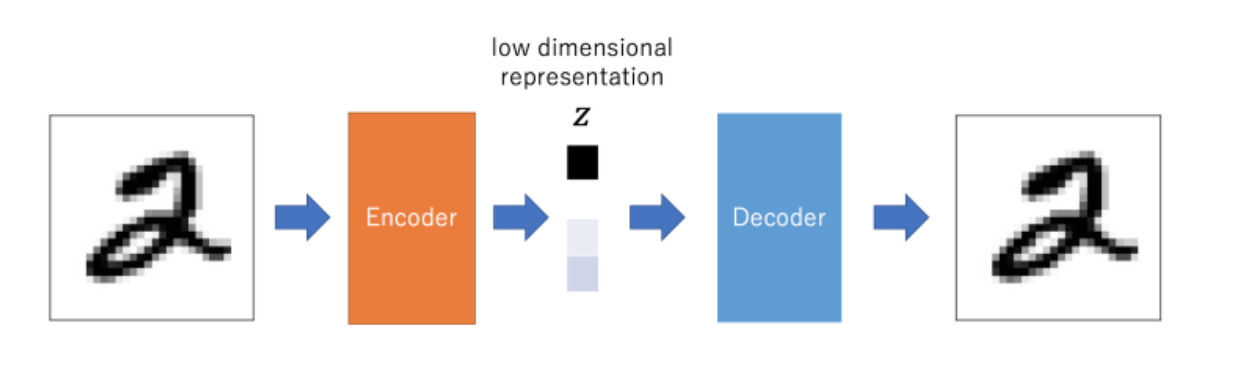
\includegraphics[width=0.7\textwidth]{autoencoder.png}
    \caption{Schema generale di un autoencoder. 
            L’encoder comprime il dato di ingresso in una rappresentazione latente a bassa 
            dimensionalità $\mathbf{z}$, mentre il decoder utilizza tale rappresentazione per ricostruire l’input originale. 
            L’addestramento avviene minimizzando l’errore di ricostruzione tra input e output, forzando la rete ad apprendere 
            una rappresentazione compatta e informativa dei dati.}
    \label{fig:autoencoder}
\end{figure}

\subsection{Bottleneck e rappresentazione latente}

La caratteristica fondamentale di un autoencoder è la presenza di uno \emph{strato centrale} a dimensionalità ridotta, 
detto \emph{bottleneck}. Questo strato impone una compressione dell'informazione, costringendo la rete ad apprendere una 
rappresentazione latente compatta dei dati.

Dal punto di vista architetturale, l'encoder implementa una funzione

\[
\highlight{
\mathbf{z} = f_1(\mathbf{x}),}
\]

che mappa l'input in uno spazio latente a bassa dimensionalità, mentre il decoder implementa una funzione

\[
\highlight{
\tilde{\mathbf{x}} = f_2(\mathbf{z}),}
\]

che ricostruisce l'input a partire dalla rappresentazione latente.

La presenza di funzioni di attivazione non lineari negli strati nascosti consente all'autoencoder di apprendere 
trasformazioni non lineari, permettendo di approssimare manifolds complessi che non possono essere catturati da tecniche lineari 
come la PCA.

\begin{figure}[H]
    \centering
    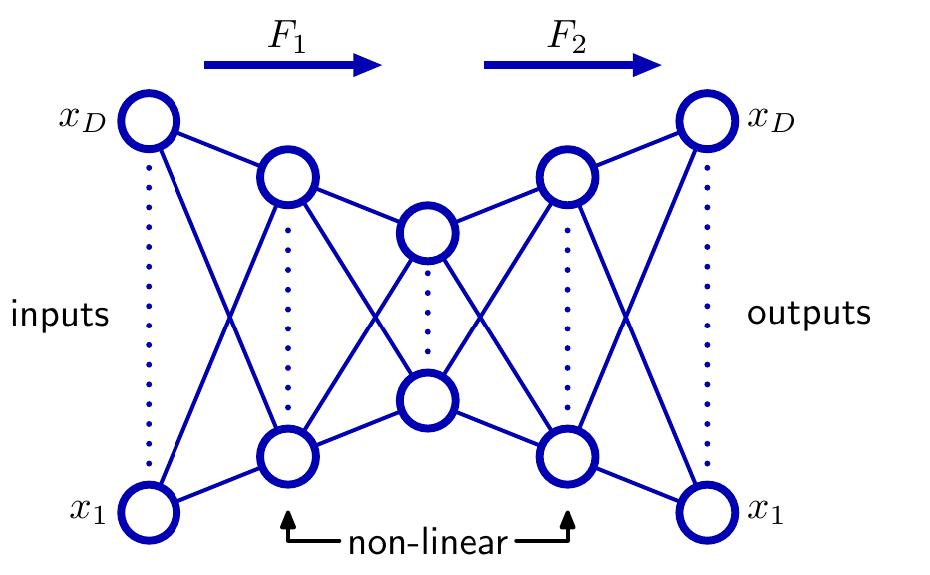
\includegraphics[width=0.7\textwidth]{bottleneck.png}
    \caption{Schema di un autoencoder con bottleneck.}
    \label{fig:bottleneck}
\end{figure}


\subsection{Convolutional Autoencoders}

Quando i dati di ingresso sono immagini, l'utilizzo di autoencoder completamente connessi risulta inefficiente, 
poiché non sfrutta la struttura spaziale dei dati. 
I \emph{Convolutional Autoencoders} (CAE) estendono il concetto di autoencoder introducendo strati convoluzionali sia 
nell'encoder sia nel decoder.

Nell'encoder, strati convoluzionali e operazioni di sottocampionamento permettono di estrarre caratteristiche locali e di 
ridurre progressivamente la dimensionalità spaziale dell'immagine, producendo una rappresentazione latente compatta. 
Il decoder opera in modo simmetrico, utilizzando strati di convoluzione trasposta (o upsampling) per ricostruire l'immagine 
originale a partire dallo spazio latente.

\begin{figure}[H]
    \centering
    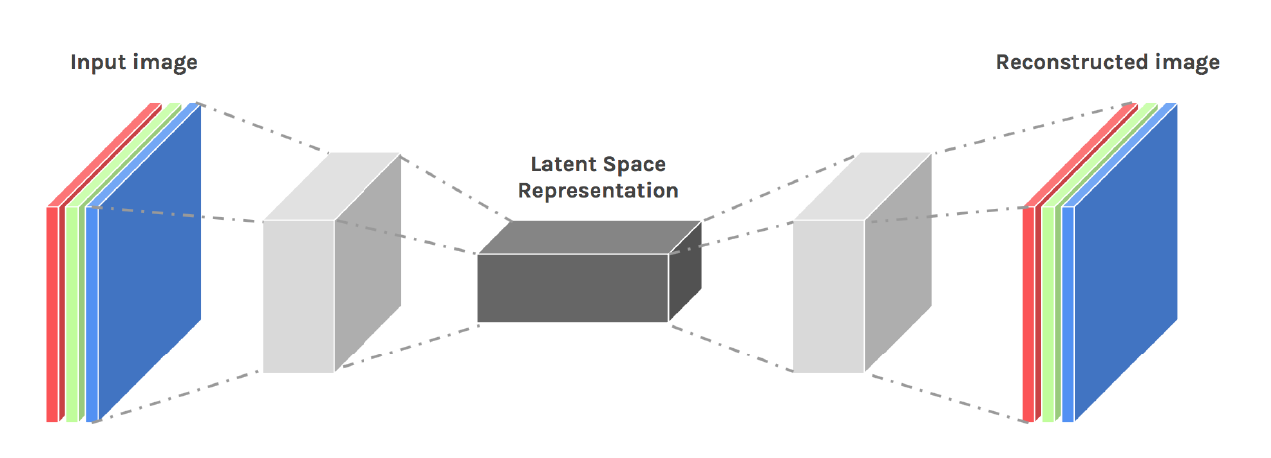
\includegraphics[width=0.7\textwidth]{convolutional_autoencoders.png}
    \caption{Schema di un Convolutional Autoencoder per immagini.}
    \label{fig:convolutional_autoencoders}
\end{figure}

\subsection{Autoencoder per Anomaly Detection}

Gli autoencoder sono particolarmente adatti a problemi di \emph{anomaly detection}, ovvero al riconoscimento di campioni a
nomali rispetto a un insieme di dati considerati normali. Questo tipo di problema può essere visto come una forma di 
classificazione a una sola classe (\emph{one-class classification}).

Si consideri un dataset
\[
\mathcal{D} = \{(\mathbf{x}_n, n)\},
\]
composto esclusivamente da campioni appartenenti alla classe normale. L'obiettivo è apprendere una funzione
\[
f : \mathcal{X} \rightarrow \{n, a\},
\]
che, dato un nuovo campione $\mathbf{x}_0$, stabilisca se esso sia normale ($n$) o anomalo ($a$).

L'approccio basato su autoencoder prevede i seguenti passi:
\begin{enumerate}
    \item addestrare un autoencoder utilizzando esclusivamente campioni normali, in modo che la rete apprenda una rappresentazione latente e una ricostruzione accurata dei dati nominali;
    \item calcolare l'errore di ricostruzione sui dati di training e determinare una soglia $\delta$, ad esempio
    \[
    \delta = \text{mean}(\mathcal{L}) + \text{std}(\mathcal{L}),
    \]
    dove $\mathcal{L}$ indica la loss di ricostruzione;
    \item dato un nuovo campione $\mathbf{x}_0$, ricostruirlo tramite l'autoencoder e calcolare l'errore di ricostruzione $\mathcal{L}_0$;
    \item se $\mathcal{L}_0 < \delta$, il campione viene classificato come normale, altrimenti come anomalo.
\end{enumerate}

L'idea alla base di questo metodo è che l'autoencoder, essendo stato addestrato solo su dati normali, 
sia in grado di ricostruire accuratamente tali campioni, mentre produca un errore elevato su dati che si discostano 
significativamente dalla distribuzione appresa.

\section{Variational Autoencoders}

I \emph{Variational Autoencoders} (VAE) sono una classe di autoencoder progettati per apprendere non solo una rappresentazione 
latente compatta dei dati, ma anche una struttura probabilistica dello spazio latente. A differenza degli autoencoder standard, 
i VAE sono modelli \emph{generativi}, in grado di produrre nuovi campioni realistici a partire dallo spazio latente.

Negli autoencoder classici, l’encoder mappa un dato di ingresso in un singolo punto dello spazio latente. Nei VAE, invece, 
l’encoder produce una \emph{distribuzione} nello spazio latente, tipicamente una distribuzione gaussiana, da cui vengono 
estratti i campioni utilizzati dal decoder.

In particolare, dato un input $\mathbf{x}$, l’encoder stima i parametri di una distribuzione

\[
\highlight{
q(\mathbf{z} \mid \mathbf{x}) = \mathcal{N}(\mathbf{z}; \boldsymbol{\mu}(\mathbf{x}), \boldsymbol{\Sigma}(\mathbf{x})),}
\]

mentre il decoder definisce una distribuzione

\[
\highlight{
p(\mathbf{x} \mid \mathbf{z}),}
\]

che modella il processo di generazione dei dati a partire dalle variabili latenti.

Una delle proprietà fondamentali dei Variational Autoencoders è la possibilità di interpretare e manipolare lo spazio 
latente in modo continuo e semanticamente significativo. Questo consente di modificare specifiche caratteristiche dei dati 
generati agendo lungo particolari direzioni dello spazio latente.

\begin{figure}[H]
    \centering
    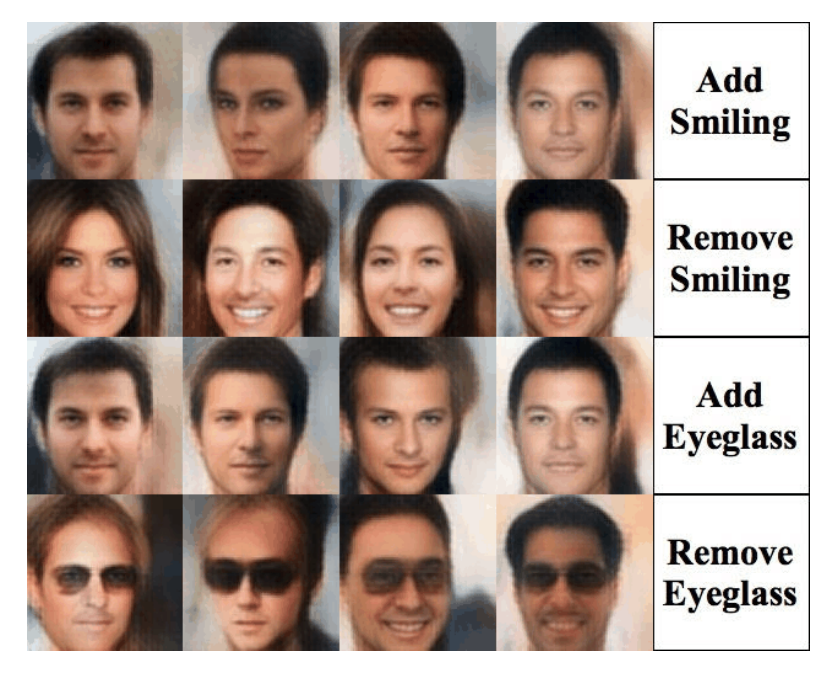
\includegraphics[width=0.7\textwidth]{VAE_faces.png}
    \caption{Esempio di manipolazione dello spazio latente in un Variational Autoencoder. 
            Variazioni controllate delle variabili latenti permettono di modificare attributi semantici delle immagini generate, 
            come l’aggiunta o la rimozione del sorriso o degli occhiali.}
    \label{fig:convolutional_autoencoders}
\end{figure}

\subsection{Problemi dei VAE e funzione obiettivo}

La formulazione dei Variational Autoencoders introduce alcune problematiche fondamentali che richiedono soluzioni specifiche.

\paragraph{Produzione di una distribuzione latente.}
A differenza degli autoencoder standard, l’encoder di un VAE non produce un singolo punto nello spazio latente, 
ma i parametri di una distribuzione, tipicamente una gaussiana:

\[
\highlight{
q(\mathbf{z} \mid \mathbf{x}) = \mathcal{N}(\mathbf{z}; \boldsymbol{\mu}(\mathbf{x}), \boldsymbol{\Sigma}(\mathbf{x})).}
\]
Questo consente di modellare l’incertezza sulla rappresentazione latente associata a ciascun dato.

\paragraph{Regolarizzazione dello spazio latente.}
Senza ulteriori vincoli, le distribuzioni latenti apprese potrebbero essere disorganizzate o degeneri, rendendo impossibile una 
generazione coerente di nuovi campioni. Per evitare questo problema, nei VAE si impone che la distribuzione latente appresa sia 
vicina a una distribuzione prior fissata, generalmente

\[
\highlight{
p(\mathbf{z}) = \mathcal{N}(\mathbf{0}, \mathbf{I}).}
\]

Questa regolarizzazione è ottenuta introducendo un termine di divergenza di Kullback--Leibler tra la distribuzione latente 
appresa e il prior:

\[
\highlight{
\mathrm{KL}\bigl(q(\mathbf{z} \mid \mathbf{x}) \,\|\, p(\mathbf{z})\bigr).}
\]

\paragraph{Evidence Lower Bound (ELBO).}
La funzione obiettivo dei VAE è data dalla \emph{Evidence Lower Bound} (ELBO), che bilancia accuratezza di ricostruzione e 
regolarizzazione dello spazio latente:

\[
\highlight{
\mathcal{L}_{\text{ELBO}} =
\mathbb{E}_{q(\mathbf{z} \mid \mathbf{x})}
\bigl[\log p(\mathbf{x} \mid \mathbf{z})\bigr]
-
\mathrm{KL}\bigl(q(\mathbf{z} \mid \mathbf{x}) \,\|\, p(\mathbf{z})\bigr).}
\]

Il primo termine incoraggia una buona ricostruzione dei dati, mentre il secondo impone una struttura continua e ben organizzata 
nello spazio latente.

\subsection{Problemi dei VAE e funzione obiettivo}

La formulazione dei Variational Autoencoders introduce alcune problematiche fondamentali che richiedono soluzioni specifiche.

\paragraph{Produzione di una distribuzione latente.}
A differenza degli autoencoder standard, l’encoder di un VAE non produce un singolo punto nello spazio latente, ma i parametri di 
una distribuzione, tipicamente una gaussiana:

\[
q(\mathbf{z} \mid \mathbf{x}) = \mathcal{N}(\mathbf{z}; \boldsymbol{\mu}(\mathbf{x}), \boldsymbol{\Sigma}(\mathbf{x})).
\]
Questo consente di modellare l’incertezza sulla rappresentazione latente associata a ciascun dato.

\paragraph{Regolarizzazione dello spazio latente.}
Senza ulteriori vincoli, le distribuzioni latenti apprese potrebbero essere disorganizzate o degeneri, rendendo impossibile una generazione coerente di nuovi campioni. Per evitare questo problema, nei VAE si impone che la distribuzione latente appresa sia vicina a una distribuzione prior fissata, generalmente
\[
p(\mathbf{z}) = \mathcal{N}(\mathbf{0}, \mathbf{I}).
\]

Questa regolarizzazione è ottenuta introducendo un termine di divergenza di Kullback--Leibler tra la distribuzione latente appresa e il prior:
\[
\mathrm{KL}\bigl(q(\mathbf{z} \mid \mathbf{x}) \,\|\, p(\mathbf{z})\bigr).
\]

\paragraph{Evidence Lower Bound (ELBO).}
La funzione obiettivo dei VAE è data dalla \emph{Evidence Lower Bound} (ELBO), che bilancia accuratezza di ricostruzione e regolarizzazione dello spazio latente:
\[
\mathcal{L}_{\text{ELBO}} =
\mathbb{E}_{q(\mathbf{z} \mid \mathbf{x})}
\bigl[\log p(\mathbf{x} \mid \mathbf{z})\bigr]
-
\mathrm{KL}\bigl(q(\mathbf{z} \mid \mathbf{x}) \,\|\, p(\mathbf{z})\bigr).
\]

Il primo termine incoraggia una buona ricostruzione dei dati, mentre il secondo impone una struttura continua e ben organizzata 
nello spazio latente.

\subsection{Reparameterization Trick}

Nei Variational Autoencoders, il decoder opera su campioni estratti dalla distribuzione latente
\[
q(\mathbf{z} \mid \mathbf{x}) = \mathcal{N}(\mathbf{z}; \boldsymbol{\mu}(\mathbf{x}), \boldsymbol{\Sigma}(\mathbf{x})).
\]
Tuttavia, l’operazione di campionamento non è differenziabile e impedirebbe l’uso diretto dell’algoritmo di backpropagation per 
l’addestramento della rete.

Per risolvere questo problema, nei VAE si introduce il \emph{reparameterization trick}, che consente di separare la componente 
stocastica dai parametri della distribuzione. In particolare, un campione $\mathbf{z}$ può essere riscritto come

\[
\highlight{
\mathbf{z} = \boldsymbol{\mu}(\mathbf{x}) + \boldsymbol{\sigma}(\mathbf{x}) \odot \boldsymbol{\epsilon},
\qquad
\boldsymbol{\epsilon} \sim \mathcal{N}(\mathbf{0}, \mathbf{I}),}
\]

dove $\boldsymbol{\sigma}$ è la deviazione standard e $\odot$ denota il prodotto elemento per elemento.

In questo modo, la variabilità stocastica è interamente contenuta nella variabile casuale $\boldsymbol{\epsilon}$, 
mentre $\boldsymbol{\mu}$ e $\boldsymbol{\sigma}$ rimangono funzioni deterministiche e differenziabili dell’input. 
Ciò permette di propagare il gradiente attraverso il campionamento e di addestrare il modello tramite discesa del gradiente.

Il reparameterization trick rappresenta un elemento chiave dei VAE e rende possibile l’ottimizzazione della funzione obiettivo 
ELBO mediante metodi di apprendimento standard.

\section{Generative Adversarial Networks}

I \emph{Generative Adversarial Networks} (GAN) sono modelli generativi che apprendono la distribuzione dei dati attraverso un processo di addestramento avversario. A differenza dei Variational Autoencoders, i GAN non modellano esplicitamente una distribuzione di probabilità dei dati, ma imparano a generare campioni realistici tramite la competizione tra due reti neurali.

Un GAN è composto da due modelli:
\begin{itemize}
    \item un \textbf{generatore} ($G$), che riceve in input un vettore latente casuale $\mathbf{z}$ e produce un campione sintetico $\tilde{\mathbf{x}} = G(\mathbf{z})$;
    
   \begin{figure}[H]
        \centering
        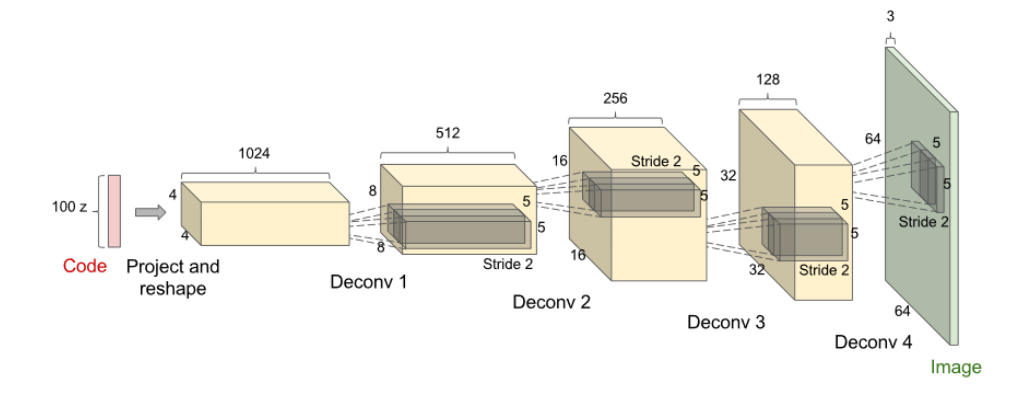
\includegraphics[width=0.8\textwidth]{gan_decoder.png}
        \label{fig:gan_decoder}
    \end{figure}

    Il generatore riceve in input un vettore latente casuale, campionato da una distribuzione semplice, e lo trasforma progressivamente in un’immagine attraverso una serie di convoluzioni trasposte e operazioni di upsampling. A partire da una rappresentazione compatta e priva di struttura spaziale, la rete costruisce l’immagine aumentando gradualmente la risoluzione e introducendo dettagli sempre più complessi.
    Il ruolo del generatore è quello di trasformare il rumore in campioni che approssimino la distribuzione dei dati reali.

    \item un \textbf{discriminatore} ($D$), che riceve in input un campione e restituisce la probabilità che esso provenga dal dataset reale piuttosto che dal generatore.


    \begin{figure}[H]
        \centering
        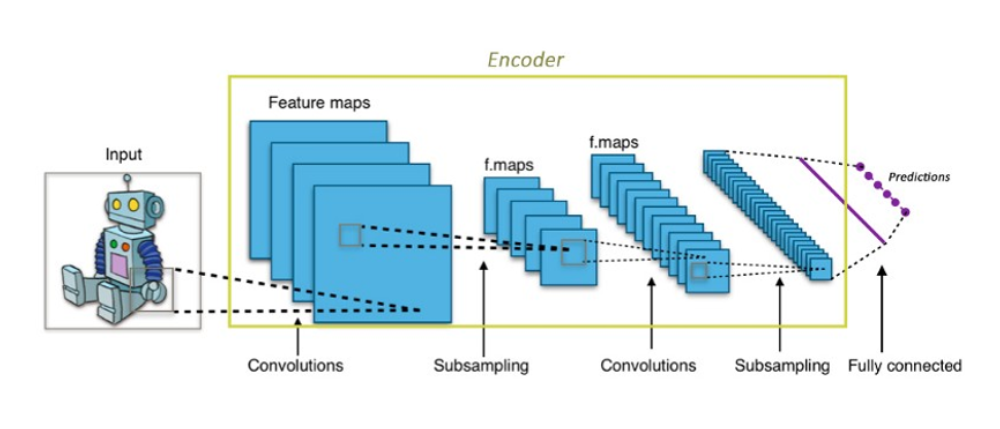
\includegraphics[width=0.8\textwidth]{gan_encoder.png}
        \label{fig:gan_encoder}
    \end{figure}

    Nei GAN, il discriminatore è tipicamente implementato come una rete convoluzionale profonda che estrae feature gerarchiche dalle immagini per distinguere campioni reali da campioni generati. Il generatore, invece, utilizza una struttura convoluzionale inversa per produrre immagini a partire da uno spazio latente.

\end{itemize}


\subsection{Addestramento avversario}

L’addestramento dei GAN si basa su un gioco competitivo tra generatore e discriminatore. Il discriminatore viene addestrato per distinguere correttamente tra campioni reali e campioni generati, mentre il generatore viene addestrato per produrre campioni in grado di ingannare il discriminatore.

Il processo di addestramento procede iterativamente secondo i seguenti passi:
\begin{enumerate}
    \item il discriminatore viene addestrato utilizzando un insieme di campioni reali e un insieme di campioni generati;
    \item il generatore viene aggiornato mantenendo fisso il discriminatore, con l’obiettivo di massimizzare la probabilità che i campioni generati vengano classificati come reali.
\end{enumerate}

Questo meccanismo competitivo porta idealmente a una situazione di equilibrio in cui il discriminatore non è più in grado di distinguere tra dati reali e dati generati, e i campioni prodotti dal generatore seguono la stessa distribuzione dei dati osservati.

\begin{figure}[H]
        \centering
        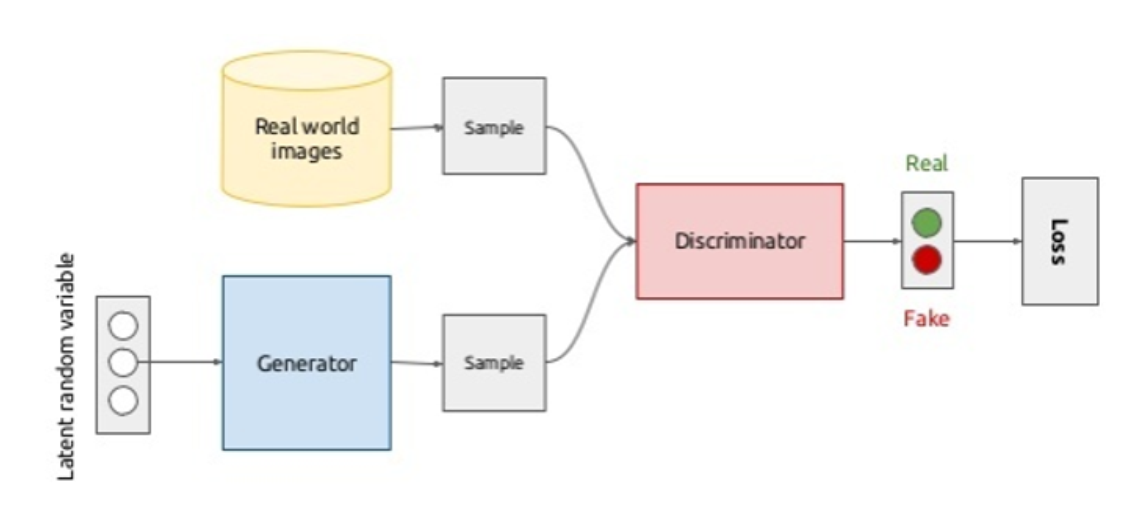
\includegraphics[width=0.90\textwidth]{GAN.png}
        \caption{Schema di addestramento di un GAN. Il generatore trasforma rumore latente in immagini, mentre il discriminatore distingue tra dati reali e generati.}
        \label{fig:GAN}
    \end{figure}

\subsection{Spazio latente nei GAN}

Anche nei GAN è presente uno spazio latente, rappresentato dal vettore $\mathbf{z}$. Tuttavia, a differenza dei Variational Autoencoders, lo spazio latente dei GAN non è regolarizzato esplicitamente e non è garantito che possieda una struttura continua o semanticamente interpretabile.

Lo spazio latente nei GAN funge principalmente da sorgente di variabilità per la generazione dei dati, consentendo di produrre campioni diversi a partire da input casuali differenti.

\subsection{Vantaggi e limiti}

I GAN sono noti per la loro capacità di generare campioni di elevata qualità percettiva, in particolare nel dominio delle immagini. Tuttavia, l’addestramento avversario può risultare instabile e non fornisce una misura esplicita della verosimiglianza dei dati.

Queste caratteristiche rendono i GAN complementari ai Variational Autoencoders: mentre i VAE privilegiano la stabilità e l’interpretabilità dello spazio latente, i GAN puntano alla qualità visiva dei campioni generati.

\newpage
\section*{RIEPILOGO}

\begin{tcolorbox}[
    colback=green!5,
    colframe=green!50!black,
    title=Convolutional Neural Networks,
    breakable
]

La riduzione della dimensionalità si basa sull’osservazione che dati ad alta dimensionalità presentano spesso una struttura intrinseca a bassa dimensionalità, descrivibile tramite variabili latenti e manifolds. L’obiettivo è individuare rappresentazioni compatte che preservino l’informazione rilevante dei dati.

La \emph{Principal Component Analysis} (PCA) realizza una riduzione dimensionale lineare proiettando i dati lungo le direzioni di massima varianza. Essa è equivalente alla minimizzazione dell’errore di ricostruzione, che risulta pari alla somma degli autovalori scartati della matrice di covarianza.

La \emph{Probabilistic PCA} fornisce un’interpretazione statistica della PCA introducendo un modello generativo lineare con variabili latenti gaussiane. In questo contesto, la PCA emerge come soluzione di massima verosimiglianza e può essere stimata tramite l’algoritmo EM.

Gli \emph{autoencoder} generalizzano la PCA introducendo modelli non lineari basati su reti neurali, composti da un encoder e un decoder separati da un bottleneck. Essi apprendono rappresentazioni latenti compatte ottimizzando una loss di ricostruzione e trovano applicazione, tra l’altro, nell’anomaly detection.

I \emph{Variational Autoencoders} (VAE) estendono gli autoencoder introducendo una formulazione probabilistica dello spazio latente. L’addestramento avviene massimizzando l’ELBO, che bilancia accuratezza di ricostruzione e regolarizzazione tramite la KL divergence. Il reparameterization trick consente l’ottimizzazione tramite backpropagation.

I \emph{Generative Adversarial Networks} (GAN) sono modelli generativi basati su un addestramento avversario tra un generatore e un discriminatore. Essi non modellano esplicitamente una likelihood, ma apprendono a generare campioni realistici tramite un gioco competitivo, privilegiando la qualità percettiva dei dati generati.

Nel complesso, queste tecniche mostrano come la modellazione dello spazio latente costituisca un elemento centrale per l’analisi, la compressione e la generazione dei dati complessi.

\end{tcolorbox}

\chapter{Reinforcement learning}

\section{Dynamic Systems e Proprietà di Markov}

Un sistema dinamico è un sistema che evolve nel tempo secondo una legge di transizione.
Indichiamo con $x_k$ lo stato del sistema al tempo $k$ e con $z_k$ l'osservazione
disponibile all'agente. L'evoluzione del sistema è descritta da:
\begin{itemize}
    \item una funzione di transizione dello stato $f$;
    \item una funzione di osservazione $h$;
    \item termini di rumore $w_k$ e $v_k$.
\end{itemize}

Si distinguono due problemi fondamentali:
\begin{itemize}
    \item \textbf{Reasoning}: dato il modello $(f,h)$ e lo stato corrente, prevedere
    gli stati futuri;
    \item \textbf{Learning}: determinare il modello $(f,h)$ a partire
    dall'esperienza passata.
\end{itemize}

Lo \textbf{stato} di un sistema dinamico deve codificare tutta l'informazione
necessaria per prevedere l'evoluzione futura del sistema, rappresentare la conoscenza acquisita e perseguire l'obiettivo dell'agente.

\subsection{Proprietà di Markov}

Un processo soddisfa la proprietà di Markov se, una volta noto lo stato corrente,
l'evoluzione futura del sistema è indipendente dalla storia passata.
In altre parole, lo stato corrente contiene tutta l'informazione necessaria
per predire il futuro.

\section{Markov Decision Processes}

Un Markov Decision Process (MDP) è un modello matematico per il
decision making sequenziale in sistemi dinamici completamente osservabili.
Negli MDP non è necessario introdurre osservazioni esplicite, poiché lo stato
del sistema è interamente accessibile all'agente.

\subsection{Modello grafico}

La Figura~\ref{fig:mdp_graph} mostra il modello grafico di un MDP.
Lo stato successivo $x_{t+1}$ dipende esclusivamente dallo stato corrente $x_t$
e dall'azione $a_t$ eseguita dall'agente.

\begin{figure}[h]
    \centering
    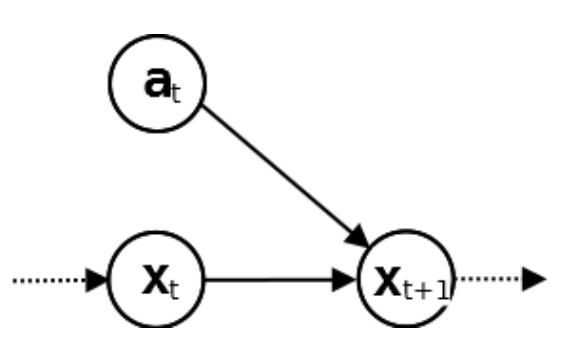
\includegraphics[width=0.5\textwidth]{mdp_graph.png}
    \caption{Modello grafico di un Markov Decision Process: lo stato successivo
    dipende dallo stato corrente e dall'azione scelta.}
    \label{fig:mdp_graph}
\end{figure}

Questo modello soddisfa la proprietà di Markov:

\[
\highlight{
P(x_{t+1} \mid x_t, a_t, x_{t-1}, a_{t-1}, \dots) =
P(x_{t+1} \mid x_t, a_t)}
\]

\subsection{Definizione formale}

Un MDP deterministico è definito come una tupla:

\[
\highlight{
\mathcal{M} = \langle X, A, \delta, r \rangle}
\]

dove:
\begin{itemize}
    \item $X$ è l'insieme finito degli stati;
    \item $A$ è l'insieme finito delle azioni;
    \item $\delta : X \times A \rightarrow X$ è la funzione di transizione;
    \item $r : X \times A \rightarrow \mathbb{R}$ è la funzione di ricompensa.
\end{itemize}

L'evoluzione del sistema è descritta dalle equazioni:

\[
\highlight{
x_{t+1} = \delta(x_t, a_t), \qquad r_t = r(x_t, a_t)}
\]

\paragraph{Learning rate}
Il learning rate $\alpha \in (0,1]$ controlla quanto le nuove osservazioni influenzano l’aggiornamento dei valori $Q$. Un valore elevato di $\alpha$ permette un apprendimento più rapido ma meno stabile, mentre un valore più piccolo rende l’apprendimento più lento ma più stabile. Se non specificato, il learning rate si assume costante.


\section{MDP}

Nei Markov Decision Processes non deterministici, l'esecuzione di una stessa
azione in uno stesso stato può portare a esiti diversi. Questo modello è più
realistico rispetto al caso deterministico e consente di rappresentare
ambienti incerti.

\subsection{MDP non deterministico}

Un MDP non deterministico è definito come una tupla:

\[
\highlight{
\mathcal{M} = \langle X, A, \delta, r \rangle}
\]

dove:
\begin{itemize}
    \item $X$ è l'insieme finito degli stati;
    \item $A$ è l'insieme finito delle azioni;
    \item $\delta : X \times A \rightarrow 2^X$ è la funzione di transizione;
    \item $r : X \times A \times X \rightarrow \mathbb{R}$ è la funzione di ricompensa.
\end{itemize}

L'evoluzione del sistema è descritta da:

\[
\highlight{
x_{t+1} \in \delta(x_t, a_t)}
\]

\subsection{MDP stocastico}

Nel caso stocastico, le transizioni sono modellate tramite una distribuzione
di probabilità. Un MDP stocastico è definito come:

\[
\highlight{
\mathcal{M} = \langle X, A, P, r \rangle}
\]

dove $P(x' \mid x, a)$ rappresenta la probabilità di transizione dallo stato
$x$ allo stato $x'$ eseguendo l'azione $a$.

La dinamica del sistema è:

\[
\highlight{
x_{t+1} \sim P(\cdot \mid x_t, a_t)}
\]

In entrambi i casi, si assume che lo stato risultante dall'esecuzione di
un'azione sia completamente osservabile.

\paragraph{NOTA BENE:}
Un problema si dice stocastico quando l’esito di un’azione non è deterministico. Questo significa che, a parità di stato e di azione, il sistema può evolvere in modi diversi a causa della presenza di fenomeni casuali. In questi casi, il comportamento dell’ambiente non è completamente prevedibile e deve essere descritto in termini probabilistici.
Formalmente: l’evoluzione del sistema o la ricompensa sono governate da variabili aleatorie.

\subsection{Esempio di MDP non deterministico: Grid World}

Consideriamo un ambiente a griglia in cui l'obiettivo dell'agente è
raggiungere la colonna più a destra partendo da qualunque stato iniziale.
Il problema è modellato come un Markov Decision Process non deterministico
\[
\mathcal{M} = \langle X, A, \delta, r \rangle .
\]

\begin{figure}[h]
    \centering
    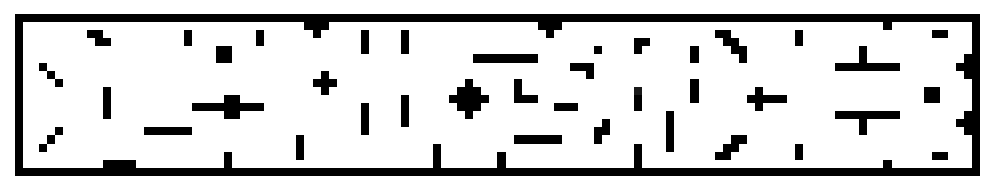
\includegraphics[width=0.95\textwidth]{nd_grid_world.png}
    \caption{Esempio di ambiente non deterministico: l'agente deve raggiungere
    il lato destro della griglia evitando gli ostacoli.}
    \label{fig:nd_grid_world}
\end{figure}

L'insieme degli stati è definito come:
\[
X = \{(r,c) \mid (r,c) \text{ coordinate nella griglia}\}.
\]

L'insieme delle azioni disponibili è:
\[
A = \{\text{Left}, \text{Right}\}.
\]

La funzione di transizione $\delta$ è non deterministica:
l'esecuzione di un'azione produce un movimento cardinale, ma con una
probabilità pari a $0.1$ l'agente si muove diagonalmente. Inoltre, se lo
stato di destinazione corrisponde a una cella occupata da un ostacolo,
l'agente rimane nello stato corrente.

La funzione di ricompensa è definita come segue:
\begin{itemize}
    \item $+1000$ per il raggiungimento della colonna più a destra;
    \item $-10$ per l'urto contro un ostacolo;
    \item $+1$ per ogni azione \emph{Right};
    \item $-1$ per ogni azione \emph{Left}.
\end{itemize}

Questo esempio evidenzia come, in presenza di transizioni non deterministiche,
l'ottimalità di una policy sia definita in termini di valore atteso della
ricompensa cumulativa e non in base all'esito deterministico delle singole
azioni.

\section{Policy}

In un Markov Decision Process, una policy descrive il comportamento
dell'agente specificando quale azione eseguire in ogni stato.
Formalmente, una policy è una funzione:

\[
\highlight{
\pi : X \rightarrow A}
\]
che associa a ogni stato $x \in X$ un'azione $\pi(x) \in A$.

Nel seguito si considerano policy stazionarie e deterministiche. Per
MDP a orizzonte infinito, esiste sempre almeno una policy stazionaria
ottima.

\subsection{Funzione valore}

Data una policy $\pi$, la funzione valore $V^\pi(x)$ è definita come
il valore atteso della ricompensa cumulativa scontata:

\[
\highlight{
V^\pi(x) \triangleq \mathbb{E}\left[\sum_{t=0}^{\infty} \gamma^t r_t
\;\middle|\; x_0 = x, \pi \right],}
\]
dove $r_t = r(x_t, a_t, x_{t+1})$, $a_t = \pi(x_t)$ e
$\gamma \in [0,1]$ è il fattore di sconto.

\subsection{Policy ottima}

Una policy $\pi^*$ è detta ottima se massimizza la funzione valore
per ogni stato:

\[
\highlight{
V^{\pi^*}(x) \geq V^\pi(x), \quad \forall x \in X, \; \forall \pi .}
\]

Equivalentemente, la policy ottima può essere definita come:

\[
\highlight{
\pi^* = \arg\max_\pi V^\pi(x), \quad \forall x \in X .}
\]

Nel caso non deterministico o stocastico, l'ottimalità è definita in termini di valore atteso della ricompensa cumulativa e non in base all'esito deterministico delle singole azioni.


\subsubsection{Esempio-Optimal Policy}

La Figura~\ref{fig:nd_policy} mostra una politica ottima per un MDP
non deterministico. Ogni cella rappresenta uno stato del sistema,
mentre il colore indica l'azione scelta dalla policy ottima:
verde per l'azione \emph{Right}, rosso per l'azione \emph{Left}.
La presenza di azioni \emph{Left} in alcune regioni evidenzia come l'ottimalità sia definita in termini di valore atteso e non di effetto deterministico dell'azione

\begin{figure}[h]
    \centering
    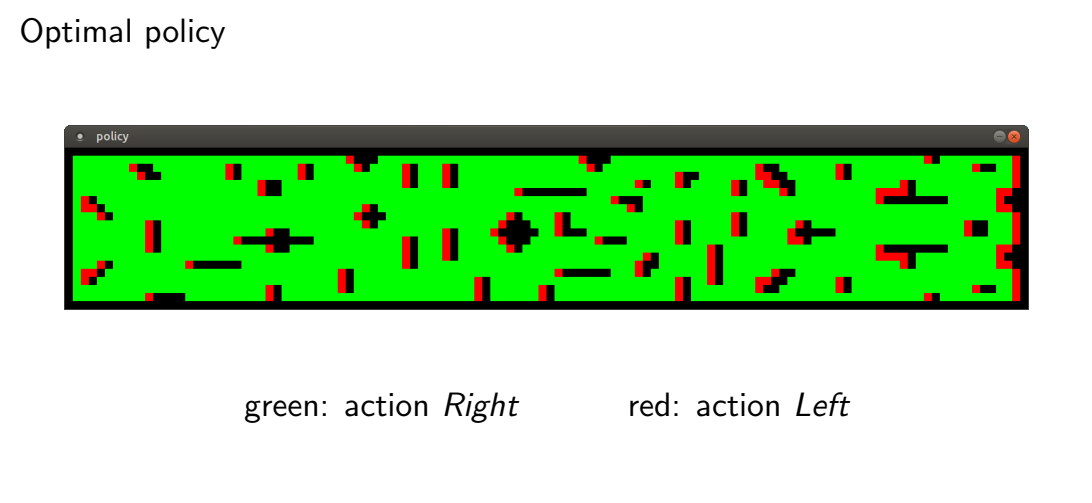
\includegraphics[width=0.9\textwidth]{nd_optimal_policy.png}
    \caption{Esempio di politica ottima in un controller non deterministico.}
    \label{fig:nd_policy}
\end{figure}

Anche se la policy è deterministica, il sistema è non deterministico:
l'esecuzione di una stessa azione nello stesso stato può portare a
stati successivi diversi. La politica ottima massimizza quindi il
valore atteso della ricompensa cumulativa e non il risultato immediato.

\section{Equazione di Bellman}

L'idea alla base dell'equazione di Bellman è che il valore di uno stato
dipende dalla ricompensa immediata ottenuta e dal valore atteso degli
stati futuri. Questa osservazione introduce una relazione ricorsiva
tra i valori degli stati.

\subsection{Equazione di Bellman per una policy}

Data una policy $\pi$, la funzione valore $V^\pi(x)$ soddisfa la seguente
equazione di Bellman:
\[
V^\pi(x) =
\mathbb{E}\left[
r(x, \pi(x), x') + \gamma V^\pi(x')
\right].
\]

Nel caso stocastico, l'equazione può essere esplicitata come:
\[
V^\pi(x) =
\sum_{x' \in X}
P(x' \mid x, \pi(x))
\left[
r(x, \pi(x), x') + \gamma V^\pi(x')
\right].
\]

\subsection{Equazione di Bellman per il valore ottimo}

La funzione valore ottima è definita come:

\[
\highlight{
V^*(x) \triangleq \max_\pi V^\pi(x).}
\]

Essa soddisfa la seguente equazione di Bellman di ottimalità:

\[
\highlight{
V^*(x) =
\max_{a \in A}
\mathbb{E}\left[
r(x, a, x') + \gamma V^*(x')
\right].}
\]

Nel caso stocastico, l'equazione assume la forma:

\[
\highlight{
V^*(x) =
\max_{a \in A}
\sum_{x' \in X}
P(x' \mid x, a)
\left[
r(x, a, x') + \gamma V^*(x')
\right].}
\]

Questa equazione non definisce un algoritmo, ma una condizione di
consistenza che il valore ottimo deve soddisfare. Gli algoritmi di
reinforcement learning mirano ad approssimare una soluzione di tale
equazione anche in assenza della conoscenza esplicita delle dinamiche
dell'ambiente.

\section{One-State Markov Decision Process}

Il One-State Markov Decision Process rappresenta il caso più semplice
di MDP e costituisce una base concettuale fondamentale per il
reinforcement learning.

Un One-State MDP è definito come:

\[
\highlight{
\mathcal{M} = \langle \{x_0\}, A, \delta, r \rangle}
\]

dove $\{x_0\}$ è l'unico stato del sistema, $A = \{a_1, \dots, a_n\}$
è l'insieme delle azioni disponibili,
$\delta(x_0, a_i) = x_0$ per ogni $a_i \in A$ e
$r(x_0, a_i, x_0) = r(a_i)$ è la funzione di ricompensa.

Poiché lo stato non cambia mai, il problema decisionale consiste
unicamente nella selezione dell'azione che massimizza la ricompensa.

\subsection{Policy ottima}

Una policy $\pi : \{x_0\} \rightarrow A$ seleziona un'unica azione.
Nel caso deterministico e noto, la policy ottima è:

\[
\highlight{
\pi^*(x_0) = \arg\max_{a_i \in A} r(a_i).}
\]

Nel caso in cui il reward sia non deterministico, la policy ottima
massimizza il valore atteso:

\[
\highlight{
\pi^*(x_0) = \arg\max_{a_i \in A} \mathbb{E}[r(a_i)].}
\]

Questo scenario introduce il problema del compromesso tra esplorazione
e sfruttamento, che costituisce il fondamento dei metodi di
reinforcement learning.

\section{Q-function}

La funzione valore $V^\pi(x)$ misura quanto sia conveniente trovarsi in
uno stato $x$ seguendo una policy $\pi$. Tuttavia, nel reinforcement
learning è spesso necessario valutare direttamente le azioni.

La Q-function associata a una policy $\pi$ è definita come:

\[
\highlight{
Q^\pi(x,a) \triangleq
\mathbb{E}\left[
r(x,a,x') + \gamma V^\pi(x')
\right]. }
\]

Essa rappresenta il valore atteso dell'esecuzione dell'azione $a$
nello stato $x$, seguita dall'applicazione della policy $\pi$.

Nel caso ottimo, la funzione valore e la Q-function sono legate da:

\[
\highlight{
V^*(x) = \max_{a \in A} Q^*(x,a).}
\]

La Q-function ottima è definita come:

\[
\highlight{
Q^*(x,a) = \max_\pi Q^\pi(x,a),}
\]
e consente di determinare direttamente la policy ottima:

\[
\highlight{
\pi^*(x) = \arg\max_{a \in A} Q^*(x,a).}
\]

La Q-function ottima soddisfa la seguente equazione di Bellman:

\[
\highlight{
Q^*(x,a) =
\mathbb{E}\left[
r(x,a,x') + \gamma \max_{a' \in A} Q^*(x',a')
\right].}
\]

\section{Q-learning e apprendimento senza modello}

Il Q-learning è un algoritmo di reinforcement learning che consente di
apprendere la Q-function ottima $Q^*(x,a)$ senza conoscere esplicitamente
il modello dell'ambiente, ovvero senza conoscere né la funzione di
transizione $\delta$ né la funzione di ricompensa $r$.

L'apprendimento avviene attraverso l'interazione diretta con l'ambiente:
l'agente esegue un'azione, osserva lo stato successivo e la ricompensa,
e aggiorna iterativamente la stima della Q-function.

\subsection{Regola di aggiornamento}

Nel caso generale non deterministico, la regola di aggiornamento del
Q-learning è:

\[
\highlight{
Q_{n}(x,a) \leftarrow
Q_{n-1}(x,a) +
\alpha \left[
r + \gamma \max_{a' \in A} Q_{n-1}(x',a')
- Q_{n-1}(x,a)
\right],}
\]

dove $x$ è lo stato corrente, $a$ l'azione eseguita, $x'$ lo stato
osservato dopo l'azione, $r$ la ricompensa immediata,
$\alpha \in (0,1]$ è il learning rate e $\gamma \in [0,1]$ è il fattore
di sconto.

Questa regola deriva direttamente dall'equazione di Bellman per la
Q-function ottima.

La regola di aggiornamento del Q-learning si applica quando il problema è modellato come un MDP con dinamica di transizione ignota e stocastica e l’agente osserva direttamente sequenze di interazione del tipo $(x,a,r,x')$. In questi casi non è possibile calcolare la funzione valore tramite le equazioni di Bellman e i valori $Q(x,a)$ devono essere appresi dall’esperienza. 

In altre parole, la regola di aggiornamento del Q-learning si usa quando l’agente non conosce il modello dell’ambiente ma può interagire con esso osservando cosa succede dopo ogni azione. In pratica, ogni volta che l’agente si trova in uno stato $x$, sceglie un’azione $a$, riceve una ricompensa $r$ e osserva il nuovo stato $x'$, si applica la formula di aggiornamento per correggere il valore $Q(x,a)$. Questa operazione viene ripetuta dopo ogni passo e permette di migliorare progressivamente la stima della funzione $Q$ a partire dall’esperienza.


\subsection{Action selection: exploration vs exploitation}

Negli algoritmi di Reinforcement Learning, oltre alla regola di aggiornamento dei valori $Q$, è necessario stabilire come l’agente seleziona le azioni durante l’apprendimento. Questo porta al problema del bilanciamento tra \emph{exploration} ed \emph{exploitation}.

Per exploitation si intende la scelta dell’azione che, sulla base delle stime correnti di $Q(x,a)$, appare come la migliore. L’exploration, invece, consiste nel provare azioni diverse per raccogliere nuove informazioni sull’ambiente ed evitare di convergere prematuramente a soluzioni subottimali. In ambienti stocastici, una strategia puramente greedy non è sufficiente.

Una soluzione semplice e ampiamente utilizzata è la \emph{$\varepsilon$-greedy policy}. Secondo questa strategia, in ogni stato $x$:
\begin{itemize}
    \item con probabilità $1 - \varepsilon$ viene selezionata l’azione che massimizza $Q(x,a)$;
    \item con probabilità $\varepsilon$ viene selezionata un’azione casuale tra quelle disponibili.
\end{itemize}

Il parametro $\varepsilon$ controlla il livello di esplorazione. All’inizio dell’apprendimento è utile scegliere un valore relativamente alto di $\varepsilon$ per favorire l’esplorazione, mentre nel tempo $\varepsilon$ può essere ridotto per privilegiare l’exploitation delle conoscenze acquisite.

Negli esercizi, la strategia $\varepsilon$-greedy viene utilizzata quando l’ambiente è stocastico e il modello non è noto, in quanto permette di apprendere efficacemente la funzione $Q$ garantendo al tempo stesso una sufficiente esplorazione dello spazio delle azioni.


Il Q-learning converge alla Q-function ottima $Q^*$ se sono soddisfatte
le seguenti condizioni:
\begin{itemize}
    \item tutte le coppie stato--azione sono visitate infinite volte;
    \item il learning rate $\alpha$ decresce in modo appropriato;
    \item il processo di apprendimento continua sufficientemente a lungo.
\end{itemize}

In tali condizioni, la policy derivata dalla Q-function approssimata
converge alla policy ottima:
\[
\pi^*(x) = \arg\max_{a \in A} Q^*(x,a).
\]

\subsection{Esempio: Slot Machine e k-Armed Bandit}

Un esempio classico di One-State Markov Decision Process è il problema
della slot machine a più leve, noto come \emph{k-armed bandit}.
In questo scenario, l'agente si trova sempre nello stesso stato $x_0$
e può scegliere una tra $n$ azioni $A = \{a_1, \dots, a_n\}$,
ciascuna corrispondente a una leva della slot machine.

\begin{figure}[h]
    \centering
    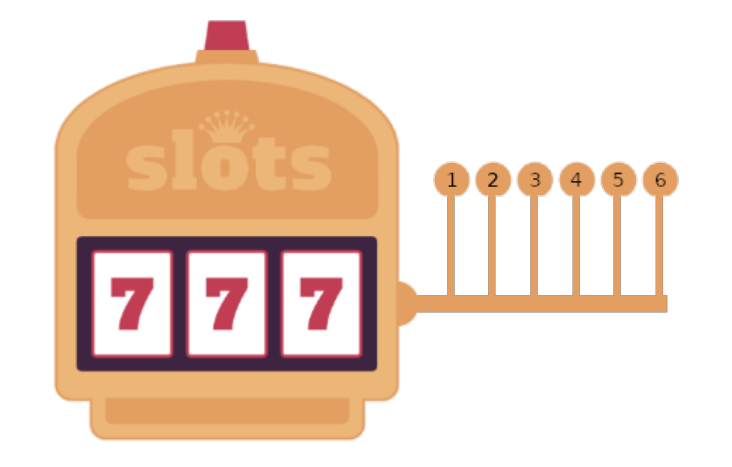
\includegraphics[width=0.55\textwidth]{k_armed_bandit.png}
    \caption{Esempio di One-State MDP: slot machine con $n$ leve.
    Ogni azione produce una ricompensa casuale, mentre lo stato
    rimane invariato.}
    \label{fig:k_armed_bandit}
\end{figure}

Il problema è modellato come un MDP:

\[
\highlight{
\mathcal{M} = \langle \{x_0\}, \{a_1, \dots, a_n\}, \delta, r \rangle}
\]

dove la funzione di transizione è definita come:

\[
\highlight{
\delta(x_0, a_i) = x_0, \quad \forall a_i \in A,}
\]

e la funzione di ricompensa dipende esclusivamente dall'azione:

\[
\highlight{
r(x_0, a_i, x_0) = r(a_i).}
\]

Le ricompense sono in generale non deterministiche e associate a
distribuzioni di probabilità ignote. L'obiettivo dell'agente è
determinare l'azione che massimizza il valore atteso della ricompensa,
bilanciando esplorazione e sfruttamento.

\subsubsection{Q-function nel k-armed bandit}

Nel caso del k-armed bandit, essendo presente un solo stato $s$,
la funzione valore azione (Q-function) si riduce a una funzione
dipendente esclusivamente dall’azione:

\[
\highlight{
Q(s,a) \equiv Q(a)}
\]

La Q-function rappresenta il valore atteso della ricompensa ottenuta
se viene selezionata l’azione $a$:

\[
\highlight{
Q(a) = \mathbb{E}[r \mid a]}
\]

Poiché le distribuzioni di ricompensa associate alle azioni sono
sconosciute, la Q-function non è nota e deve essere stimata a partire
dall’esperienza.

\subsection{Problema e concetto di soluzione}

Il problema del k-armed bandit consiste nello stimare la Q-function
associata a ciascuna azione e nel selezionare una policy che massimizzi
la ricompensa attesa cumulativa.

Una policy $\pi$ associa a ogni istante temporale un’azione da eseguire.
Nel caso ideale, la policy ottima seleziona sempre l’azione con valore
atteso massimo:

\[
\highlight{
\pi^* = \arg\max_{a \in \mathcal{A}} Q(a)}
\]

Tuttavia, poiché i valori $Q(a)$ sono inizialmente ignoti, l’agente deve
bilanciare:
\begin{itemize}
\item \emph{exploration}: selezionare azioni poco esplorate per migliorare
la stima di $Q(a)$;
\item \emph{exploitation}: selezionare l’azione che massimizza la stima
corrente di $Q(a)$.
\end{itemize}

\subsubsection{Apprendimento della Q-function}

La stima della Q-function può essere aggiornata incrementalmente
utilizzando una regola di apprendimento di tipo reinforcement learning.
Dopo aver selezionato l’azione $a_t$ e osservato la ricompensa $r_t$,
la stima viene aggiornata come:
\[
Q_{t+1}(a_t) = Q_t(a_t) + \alpha \big( r_t - Q_t(a_t) \big)
\]
dove:
\begin{itemize}
\item $\alpha \in (0,1]$ è il learning rate;
\item $r_t$ è la ricompensa osservata al tempo $t$.
\end{itemize}

Questa regola rappresenta un caso particolare del Q-learning,
semplificato dall’assenza di dinamica di stato e di ricompense future.

\section{Altri algoritmi di reinforcement learning}

Oltre al Q-learning, esistono altri algoritmi per l'apprendimento in
Markov Decision Processes non deterministici. Tra questi:
\begin{itemize}
    \item \textbf{SARSA}, un metodo \emph{on-policy} che valuta la policy
    effettivamente seguita dall'agente;
    \item \textbf{Temporal Difference} (TD), che combina idee di Monte Carlo
    e programmazione dinamica;
    \item approcci \emph{model-based}, che stimano esplicitamente il
    modello dell'ambiente per pianificare le azioni.
\end{itemize}

\newpage
\section*{RIEPILOGO}

\begin{tcolorbox}[
  colback=green!10!white,
  colframe=green!50!black,
  coltitle=white,
  title=\textbf{Reinforcement Learning – Concetti chiave},
  fonttitle=\bfseries,
  breakable
]

Il \emph{Reinforcement Learning} studia problemi decisionali sequenziali in cui
un agente apprende interagendo con un ambiente, senza disporre di esempi
supervisionati, ma solo di segnali di ricompensa.

\medskip
\textbf{Markov Decision Process (MDP)}

Un problema di reinforcement learning è formalizzato tramite un
\emph{Markov Decision Process}:
\[
\mathcal{M} = \langle \mathcal{S}, \mathcal{A}, p, r, \gamma \rangle
\]
dove:
\begin{itemize}
\item $\mathcal{S}$ è l’insieme degli stati;
\item $\mathcal{A}$ è l’insieme delle azioni;
\item $p(s' \mid s,a)$ è la probabilità di transizione;
\item $r(s,a)$ è la funzione di ricompensa;
\item $\gamma \in [0,1)$ è il fattore di sconto.
\end{itemize}

La proprietà di Markov implica che l’evoluzione futura del sistema dipende
solo dallo stato corrente e dall’azione selezionata.

\medskip
\textbf{Policy e funzioni di valore}

Una \emph{policy} $\pi$ definisce il comportamento dell’agente, specificando
l’azione da eseguire in ciascuno stato.
Le prestazioni di una policy sono valutate tramite:
\begin{itemize}
\item la funzione valore di stato $V^\pi(s)$;
\item la funzione valore azione $Q^\pi(s,a)$.
\end{itemize}

La policy ottima $\pi^*$ massimizza il valore atteso cumulativo delle ricompense.

\medskip
\textbf{Equazioni di Bellman}

Le equazioni di Bellman forniscono una caratterizzazione ricorsiva delle funzioni
di valore.
Nel caso ottimo, esse esprimono il principio di ottimalità e costituiscono la base
per gli algoritmi di apprendimento e pianificazione.

\medskip
\textbf{Reinforcement Learning senza modello}

Nel reinforcement learning l’agente non conosce né le probabilità di transizione
né la funzione di ricompensa.
Gli algoritmi \emph{model-free} apprendono direttamente le funzioni di valore
a partire dall’esperienza, senza stimare esplicitamente il modello dell’ambiente.

\medskip
\textbf{Q-learning}

Il Q-learning è un algoritmo model-free che apprende la Q-function ottima
tramite aggiornamenti incrementali basati sull’errore di Bellman.
La policy è ottenuta selezionando l’azione che massimizza il valore stimato
della Q-function.

\medskip
\textbf{k-Armed Bandit}

Il k-armed bandit è un caso particolare di reinforcement learning
modellabile come MDP a singolo stato.
In questo caso la Q-function dipende solo dall’azione:
\[
Q(a) = \mathbb{E}[r \mid a]
\]

Il problema consiste nello stimare i valori attesi delle azioni e nel bilanciare
\emph{exploration} ed \emph{exploitation} per massimizzare la ricompensa cumulativa.

\medskip
\textbf{Action selection}

Poiché i valori delle azioni sono inizialmente ignoti, è necessario adottare
strategie di selezione dell’azione che consentano l’esplorazione dell’ambiente,
come ad esempio policy $\varepsilon$-greedy.

\medskip
\textbf{Obiettivo del Reinforcement Learning}

L’obiettivo finale è apprendere una policy ottima che massimizzi la somma
attesa delle ricompense nel tempo, attraverso l’interazione iterativa
con l’ambiente e l’aggiornamento delle stime di valore.

\end{tcolorbox}

\newpage
\section*{GLOSSARIO}

\begin{description}
    \item[Dataset (insieme di dati)]
Un \emph{dataset} è un insieme strutturato di istanze utilizzato per
l’addestramento, la validazione o la valutazione di un modello di Machine Learning.
Può essere visto come una tabella in cui ogni riga rappresenta un’istanza e ogni
colonna una feature.

    \item[Instance (istanza, esempio)]
Un’\emph{instance} è un singolo esempio contenuto nel dataset.
Rappresenta un caso specifico del problema e costituisce l’unità di base su cui
il modello effettua una predizione.

    \item[Feature (attributo, caratteristica)]
Una \emph{feature} è una caratteristica numerica o categoriale che descrive
un’istanza.
Ogni istanza è rappresentata da un vettore di feature che ne codifica le
proprietà rilevanti per il problema di apprendimento.

    \item[Label / Target (etichetta, valore di uscita)]
La \emph{label} (o \emph{target}) è il valore di output corretto associato a
un’istanza in un problema di \emph{supervised learning}.
Rappresenta ciò che il modello deve imparare a predire a partire dalle feature.

Nel caso di:
\begin{itemize}
\item \emph{classificazione}, la label appartiene a un insieme finito di classi;
\item \emph{regressione}, la label è un valore numerico continuo.
\end{itemize}

    \item[Model (modello)]
Un \emph{model} è una funzione, parametrica o non parametrica, che associa
le feature di un’istanza a una predizione dell’output.
Il modello rappresenta ciò che viene appreso dai dati e viene utilizzato
per effettuare predizioni su nuove istanze.

    \item[Learning Algorithm (algoritmo di apprendimento)]
Un \emph{learning algorithm} è la procedura che stima i parametri del modello
a partire dal dataset di training, ottimizzando una funzione di costo.
L’algoritmo di apprendimento non effettua predizioni, ma serve esclusivamente
a costruire o aggiornare il modello.

    \item[Prediction (predizione)]
Una \emph{prediction} è l’output prodotto dal modello quando viene applicato
a un’istanza.
La predizione rappresenta la stima del valore di output e non coincide
necessariamente con la label corretta.

    \item[Loss Function (funzione di perdita, funzione di costo)]
Una \emph{loss function} misura l’errore commesso dal modello su una singola
istanza, confrontando la predizione con la label corretta.
La loss function fornisce un segnale numerico che guida l’algoritmo di
apprendimento nel migliorare il modello durante la fase di training.

    \item[Metric (metrica di valutazione)]
Una \emph{metric} è una misura utilizzata per valutare le prestazioni complessive
di un modello su un insieme di dati.
A differenza della loss function, la metrica non viene utilizzata per
l’apprendimento del modello, ma solo per confrontare modelli o stimarne
la capacità di generalizzazione.

Esempi comuni di metriche sono l’accuracy, la precision, la recall e l’RMSE.

    \item[Training Set (insieme di addestramento)]
Il \emph{training set} è la parte del dataset utilizzata per addestrare il modello,
cioè per stimarne i parametri tramite l’algoritmo di apprendimento.
Durante il training, il modello minimizza la loss function sui dati di training.

    \item[Test Set (insieme di test)]
Il \emph{test set} è un insieme di dati separato dal training set e utilizzato
esclusivamente per valutare le prestazioni del modello su istanze non viste
durante l’addestramento.
Il test set fornisce una stima della capacità di generalizzazione del modello.

    \item[Validation Set (insieme di validazione)]
Il \emph{validation set} è un insieme di dati utilizzato durante lo sviluppo del
modello per confrontare diverse scelte progettuali, come iperparametri o architetture.
I dati di validazione non vengono usati per addestrare il modello, ma per guidarne
la selezione.

    \item[Mean (media)]
La \emph{mean} è il valore medio di un insieme di dati.
Rappresenta il “centro” dei dati, cioè il valore attorno al quale le osservazioni
tendono a concentrarsi.

    \item[Variance (varianza)]
La \emph{variance} misura quanto i dati sono dispersi attorno alla media.
Una varianza piccola indica dati molto concentrati, una varianza grande indica
dati molto sparsi.

    \item[Covariance (covarianza)]
La \emph{covariance} misura come due variabili variano insieme.
Se è positiva, le due variabili tendono ad aumentare o diminuire insieme;
se è negativa, una tende ad aumentare quando l’altra diminuisce;
se è circa zero, non c’è una relazione lineare evidente.

    \item[Covariance Matrix (matrice di covarianza)]
La \emph{covariance matrix} raccoglie tutte le covarianze tra le feature di un
dataset.
Sulla diagonale contiene le varianze delle singole feature, mentre fuori diagonale
contiene le covarianze tra coppie di feature.
Descrive la forma e l’orientamento della distribuzione dei dati.

    \item[Distribution (distribuzione di probabilità)]
Una \emph{distribution} descrive come i valori di una variabile sono
distribuiti, cioè quali valori sono più probabili e quali meno.
In altre parole, una distribuzione assegna una probabilità (o una densità)
ai possibili valori che una variabile può assumere.

Nel Machine Learning, una distribuzione viene usata per modellare i dati,
le osservazioni o le incertezze associate a un fenomeno reale.

    \item[Gaussian Distribution / Normal Distribution (distribuzione gaussiana / normale)]
La \emph{Gaussian distribution} è una distribuzione continua a forma di campana,
completamente descritta da media e varianza.
La media indica il centro della distribuzione, la varianza ne controlla la larghezza.
I termini “gaussiana” e “normale” indicano la stessa distribuzione.

    \item[Discrete Distribution (distribuzione discreta)]
Una \emph{discrete distribution} è una distribuzione di probabilità definita su un
insieme finito o numerabile di valori.
A ciascun valore è associata una probabilità, e la somma di tutte le probabilità
è pari a uno.

    \item[Observations (osservazioni)]
Le \emph{observations} sono i dati osservati, cioè i valori effettivamente misurati
o raccolti dal mondo reale.
Nel Machine Learning, le osservazioni costituiscono il dataset di training.

    \item[Weights (pesi)]
I \emph{weights} sono parametri numerici di un modello che determinano l’importanza
delle feature.
Pesi grandi indicano feature più influenti, pesi piccoli indicano feature meno
rilevanti.

    \item[Likelihood (verosimiglianza)]
La \emph{likelihood} misura quanto è plausibile osservare i dati assumendo fissati
i parametri di un modello.
Non è una probabilità dei parametri, ma una misura di quanto bene il modello
spiega i dati osservati.

    \item[Log-Likelihood (log-verosimiglianza)]
La \emph{log-likelihood} è il logaritmo della likelihood.
Viene utilizzata perché semplifica i calcoli, trasforma prodotti in somme e rende
più stabile l’ottimizzazione numerica.
Massimizzare la log-likelihood equivale a massimizzare la likelihood.

\end{description}

\begin{table}[H]
\centering
\begin{tabular}{c l l}
\toprule
\textbf{Simbolo} & \textbf{Nome} & \textbf{Significato / uso} \\
\midrule
$\land$ & AND (congiunzione) & vero se entrambi i valori sono veri \\
$\lor$ & OR (disgiunzione) & vero se almeno uno dei valori è vero \\
$\lnot$ / $\neg$ & NOT (negazione) & inverte il valore di verità \\
$\to$ & Implication (implicazione) & $A \to B$: se $A$ allora $B$ \\
$\leftrightarrow$ & Iff / Biconditional (doppia implicazione) & vero se $A$ e $B$ hanno lo stesso valore \\
$\oplus$ & XOR (exclusive or) & vero se esattamente uno è vero \\
$\forall$ & For all (per ogni) & quantificatore universale \\
$\exists$ & Exists (esiste) & quantificatore esistenziale \\
$\models$ & Entails (implica logicamente) & $A \models B$: $B$ è vero in ogni modello in cui $A$ lo è \\
$\vdash$ & Derives (derivabile) & $A \vdash B$: $B$ è deducibile da $A$ \\
\bottomrule
\end{tabular}
\caption{Simboli logici fondamentali}
\end{table}


\end{document}